\documentclass[12pt]{book}

\title{Think Java}
\author{Allen B. Downey and Chris Mayfield}

\newcommand{\thetitle}{Think Java}
\newcommand{\thesubtitle}{How to Think Like a Computer Scientist}
\newcommand{\theauthors}{Allen B. Downey and Chris Mayfield}
\newcommand{\theversion}{2nd Edition, Version 7.0.0 DRAFT}

%%%% Both LATEX and PLASTEX

\usepackage{graphicx}
\usepackage{setspace}

% automatically index glossary terms
\newcommand{\term}[1]{%
\item[#1:]\index{#1}}

\usepackage{amsmath}
\usepackage{amsthm}

% format end of chapter excercises
\newtheoremstyle{exercise}
  {12pt}        % space above
  {12pt}        % space below
  {}            % body font
  {}            % indent amount
  {\bfseries}   % head font
  {}            % punctuation
  {12pt}        % head space
  {}            % custom head
\theoremstyle{exercise}
\newtheorem{exercise}{Exercise}[chapter]

\newif\ifplastex
\plastexfalse

%%%% PLASTEX ONLY
\ifplastex

\makeindex

\usepackage{localdef}

\usepackage{url}
\renewcommand{\href}[2]{\url{#1}}

\makeatletter
\newcount\anchorcnt
\newcommand*{\Anchor}[1]{%
  \@bsphack%
    \Hy@GlobalStepCount\anchorcnt%
    \edef\@currentHref{anchor.\the\anchorcnt}%
    \Hy@raisedlink{\hyper@anchorstart{\@currentHref}\hyper@anchorend}%
    \M@gettitle{}\label{#1}%
    \@esphack%
}
\makeatother

% code listing environments:
% we don't need these for plastex because they get replaced
% by preprocess.py
%\newenvironment{code}{\begin{verbatim}}{\end{verbatim}}
%\newenvironment{stdout}{\begin{verbatim}}{\end{verbatim}}

% inline syntax formatting
\newcommand{\java}{\verb}%}
\newcommand{\textcolor}[1]{\relax}

%%%% LATEX/HTML ONLY
\else

%BEGIN LATEX
\usepackage{comment}
\excludecomment{htmlonly}
\includecomment{latexonly}
%END LATEX

\usepackage{geometry}
\geometry{
    width=5.5in,
    height=8.5in,
    hmarginratio=3:2,
    vmarginratio=1:1,
    includehead=true,
    headheight=15pt
}

% paragraph spacing
\setlength{\parindent}{0pt}                      % 17.62482pt
\setlength{\parskip}{12pt plus 4pt minus 4pt}    % 0.0pt plus 1.0pt
\linespread{1.05}
\def\arraystretch{1.5}

% list spacing
\setlength{\topsep}{5pt plus 2pt minus 3pt}      % 10.0pt plus 4.0pt minus 6.0pt
\setlength{\partopsep}{-6pt plus 2pt minus 2pt}  %  3.0pt plus 2.0pt minus 2.0pt
\setlength{\itemsep}{0pt}                        %  5.0pt plus 2.5pt minus 1.0pt

% these are copied from tex/latex/base/book.cls
% all I changed is afterskip
\makeatletter
\renewcommand{\section}{\@startsection{section}{1}{\z@}%
    {-3.5ex \@plus -1ex \@minus -.2ex}%
    {0.7ex \@plus.2ex}%
    {\normalfont\Large\bfseries}}
\renewcommand\subsection{\@startsection{subsection}{2}{\z@}%
    {-3.25ex\@plus -1ex \@minus -.2ex}%
    {0.3ex \@plus .2ex}%
    {\normalfont\large\bfseries}}
\renewcommand\subsubsection{\@startsection{subsubsection}{3}{\z@}%
    {-3.25ex\@plus -1ex \@minus -.2ex}%
    {0.3ex \@plus .2ex}%
    {\normalfont\normalsize\bfseries}}
\makeatother

% table of contents vertical spacing
\usepackage{tocloft}
\setlength\cftparskip{8pt plus 4pt minus 4pt}

% balanced index with TOC entry
\usepackage[totoc]{idxlayout}

% The following line adds a little extra space to the column
% in which the Section numbers appear in the table of contents
\makeatletter
\renewcommand{\l@section}{\@dottedtocline{1}{1.5em}{3.0em}}
\makeatother

% customize page headers
\usepackage{fancyhdr}
\pagestyle{fancyplain}
\renewcommand{\chaptermark}[1]{\markboth{Chapter \thechapter ~~ #1}{}}
\renewcommand{\sectionmark}[1]{\markright{\thesection ~~ #1}}
\lhead[\fancyplain{}{\bfseries\thepage}]%
      {\fancyplain{}{\bfseries\rightmark}}
\rhead[\fancyplain{}{\bfseries\leftmark}]%
      {\fancyplain{}{\bfseries\thepage}}
\cfoot{}
\usepackage[mmddyyyy]{datetime}
\rfoot{\textcolor{gray}{\tiny \thetitle, \theversion, \today}}

%% tweak spacing of figures and captions
%\usepackage{floatrow}
%\usepackage{caption}
%\captionsetup{
%    font=small,
%    labelformat=empty,
%    justification=centering,
%    skip=4pt
%}

% colors for code listings and output
\usepackage{xcolor}
\definecolor{bgcolor}{HTML}{FAFAFA}
\definecolor{comment}{HTML}{007C00}
\definecolor{keyword}{HTML}{0000FF}
\definecolor{strings}{HTML}{B20000}

% syntax highlighting in code listings
\usepackage{textcomp}
\usepackage{listings}
\lstset{
    language=java,
    basicstyle=\ttfamily,
    backgroundcolor=\color{bgcolor},
    commentstyle=\color{comment},
    keywordstyle=\color{keyword},
    stringstyle=\color{strings},
    columns=fullflexible,
    emph={label},  % keyword?
    keepspaces=true,
    showstringspaces=false,
    upquote=true,
    xleftmargin=15pt,  % \parindent
    framexleftmargin=3pt,
    aboveskip=\parskip,
    belowskip=\parskip
}

% code listing environments
\lstnewenvironment{code}
{\minipage{\linewidth}}
{\endminipage}
\lstnewenvironment{stdout}
{\lstset{commentstyle=,keywordstyle=,stringstyle=}\minipage{\linewidth}}
{\endminipage}

% interactive code listing
\lstnewenvironment{trinket}[2][400]
{\minipage{\linewidth}}
{\endminipage}

% inline syntax formatting
\newcommand{\java}[1]{\lstinline{#1}}%{

% prevent hyphens in names
\hyphenation{DrJava}
\hyphenation{GitHub}
\hyphenation{Javadoc}

% pdf hyperlinks, table of contents, and document properties
\usepackage{hyperref}
\hypersetup{%
  pdftitle={\thetitle: \thesubtitle},
  pdfauthor={\theauthors},
  pdfsubject={Version \theversion},
  pdfkeywords={},
  bookmarksopen=false,
  bookmarksnumbered=true,
  colorlinks=true,
  citecolor=black,
  filecolor=black,
  linkcolor=black,
  urlcolor=blue
}

% add dot after numbers in pdf bookmarks
\makeatletter
\renewcommand{\Hy@numberline}[1]{#1. }
\makeatother


\fi

%%%% END OF PREAMBLE
\begin{document}

\frontmatter

%%%% PLASTEX ONLY
\ifplastex

\maketitle

%%%% LATEX/HTML ONLY
\else

\begin{latexonly}

%--half title-------------------------------------------------
\thispagestyle{empty}

\begin{flushright}
\vspace*{2.0in}

\begin{spacing}{3}
{\huge \thetitle} \\
{\Large \thesubtitle}
\end{spacing}

\vspace{0.25in}

\theversion

\vfill
\end{flushright}

%--verso------------------------------------------------------
\newpage
\thispagestyle{empty}

\quad

%--title page-------------------------------------------------
\newpage
\thispagestyle{empty}

\begin{flushright}
\vspace*{2.0in}

\begin{spacing}{3}
{\huge \thetitle} \\
{\Large \thesubtitle}
\end{spacing}

\vspace{0.25in}

\theversion

\vspace{1in}

{\Large \theauthors}

\vspace{0.5in}

{\Large Green Tea Press}

{\small Needham, Massachusetts}

\vfill
\end{flushright}

%--copyright--------------------------------------------------
\newpage
\thispagestyle{empty}

Copyright \copyright ~2019 \theauthors.

\vspace{0.2in}

\begin{flushleft}
Green Tea Press \\
9 Washburn Ave \\
Needham, MA 02492
\end{flushleft}

Permission is granted to copy, distribute, and/or modify this work under the terms of the Creative Commons Attribution-NonCommercial-ShareAlike 4.0 International License, which is available at \url{https://creativecommons.org/licenses/by-nc-sa/4.0/}.

The original form of this book is \LaTeX\ source code.
Compiling this code has the effect of generating a device-independent representation of the book, which can be converted to other formats and printed.

The \LaTeX\ source for this book is available from \url{https://thinkjava.org/} and \url{https://github.com/ChrisMayfield/ThinkJava2}.

%--table of contents------------------------------------------

\cleardoublepage
\setcounter{tocdepth}{1}
\tableofcontents

\end{latexonly}

%--HTML title page--------------------------------------------

\begin{htmlonly}

\vspace{1em}

{\Large \thetitle: \thesubtitle}

{\large \theauthors}

\theversion

\vspace{1em}

Copyright \copyright ~2019 \theauthors.

Permission is granted to copy, distribute, and/or modify this work under the terms of the Creative Commons Attribution-NonCommercial-ShareAlike 4.0 International License, which is available at \url{https://creativecommons.org/licenses/by-nc-sa/4.0/}.

\vspace{1em}

\end{htmlonly}

%-------------------------------------------------------------

%%%% END OF THE PART WE SKIP FOR PLASTEX
\fi

\chapter*{Preface}
\label{preface}

\markboth{PREFACE}{PREFACE}
\addcontentsline{toc}{chapter}{Preface}

{\it Think Java} is an introduction to computer science and programming intended for readers with little or no experience.
We start with the most basic concepts and are careful to define all terms when they are first used.
The book presents each new idea in a logical progression.
Larger topics, like recursion and object-oriented programming, are divided into smaller examples and introduced over the course of several chapters.

This book is intentionally concise.
Each chapter is 12--14 pages and covers the material for one week of a college course.
It is not meant to be a comprehensive presentation of Java, but rather, an initial exposure to programming constructs and techniques.
We begin with small problems and basic algorithms and work up to object-oriented design.
In the vocabulary of computer science pedagogy, this book uses the ``objects late'' approach.


\section*{The philosophy behind the book}

Here are the guiding principles that make the book the way it is:

\begin{itemize}

\item {\em One concept at a time.}
We break down topics that give beginners trouble into a series of small steps, so that they can exercise each new concept in isolation before continuing.

\item {\em Balance of Java and concepts.}
The book is not primarily about Java; it uses code examples to demonstrate computer science.
Most chapters start with language features and end with concepts.

\item {\em Conciseness.}
An important goal of the book is to be small enough so that students can read and understand the entire text in a one-semester college or AP course.
%Students can read 1--2 chapters per week, depending on the pace of the instruction.

\item {\em Emphasis on vocabulary.}
We try to introduce the minimum number of terms and define them carefully when they are first used.
We also organize them in glossaries at the end of each chapter.

\item {\em Program development.}
There are many strategies for writing programs, including bottom-up, top-down, and others.
We demonstrate multiple program development techniques, allowing readers to choose methods that work best for them.

\item {\em Multiple learning curves.}
To write a program, you have to understand the algorithm, know the programming language, and be able to debug errors.
We discuss these and other aspects throughout the book, and include an appendix that summarizes our advice.

%\item {\em Spiral approach.}
%Some concepts take time to sink in.
%The more difficult ideas in the book, like recursion, appear several times.
%By coming back to these topics, we give learners a chance to review and reinforce.

%\item {\em Keep it simple.}
%We use the minimum amount of Java to get the maximum amount of programming ability.
%The goal of this book is to teach fundamental ideas from computer science, not Java.
%We leave out some language features, like the \java{switch} statement, that are unnecessary, and we present only a few of the many classes in the Java libraries.

\end{itemize}


\section*{Object-oriented programming}

Some Java books introduce classes and objects immediately; others begin with procedural programming and transition to object-oriented more gradually.

Many of Java's object-oriented features are motivated by problems with previous languages, and their implementations are influenced by this history.
Some of these features are hard to explain when people aren't familiar with the problems they solve.

We get to object-oriented programming as quickly as possible, limited by the requirement that we introduce concepts one at a time, as clearly as possible, in a way that allows readers to practice each idea in isolation before moving on.
So it takes some time to get there.

But you can't write Java programs (even hello world) without encountering object-oriented features.
In some cases we explain a feature briefly when it first appears, and then explain it more deeply later on.

This book is well suited to prepare students for the AP Computer Science A exam, which includes object-oriented design and implementation.
(AP is a registered trademark of the College Board.)
We introduce nearly every topic in the ``AP Java subset'' with a few exceptions.
A mapping of {\it Think Java} section numbers to the current AP course description is available on our website: \url{http://thinkjava.org}.


\section*{Appendixes}

The chapters of this book are meant to be read in order, because each one builds on the previous one.
We also include three appendixes with material that can be read at any time:

\begin{description}

\item{\bf Appendix A: Tools}

This appendix explains how to download and install Java so you can compile programs on your computer.
It also provides a brief introduction to DrJava -- an ``integrated development environment'' (IDE) that is designed primarily for students -- and other development tools, including Checkstyle for code quality and JUnit for testing.

\item{\bf Appendix B: Javadoc}

It's important to document your classes and methods so that other programmers (including yourself in the future) will know how to use them.
This appendix explains how to read documentation, how to write documentation, and how the Javadoc tool works.

\item{\bf Appendix C: Graphics}

Java provides libraries for working with graphics and animation, and these topics can be engaging for students.
The libraries require object-oriented features that readers will not completely understand until after Chapter~\ref{objects}, but they can be used much earlier.

\item{\bf Appendix D: Debugging}

We provide debugging suggestions throughout the book, but we also collect our debugging advice in an appendix.
We recommend that readers review this appendix several times as they work through the book.

\end{description}


\section*{Using the code examples}
\label{code}

Most of the code examples in this book are available from a Git repository at \url{https://github.com/ChrisMayfield/ThinkJavaCode2}.
Git is a ``version control system'' that allows you to keep track of the files that make up a project.
A collection of files under Git's control is called a ``repository''.

\index{repository}
\index{GitHub}

GitHub is a hosting service that provides storage for Git repositories and a convenient web interface.
It provides several ways to work with the code:

\begin{itemize}

\item You can create a copy of the repository on GitHub by pressing the {\sf Fork} button.
If you don't already have a GitHub account, you'll need to create one.
After forking, you'll have your own repository on GitHub that you can use to keep track of code you write.
Then you can ``clone'' the repository, which downloads a copy of the files to your computer.

\item Alternatively, you could clone the repository without forking.
If you choose this option, you don't need a GitHub account, but you won't be able to save your changes on GitHub.

\item If you don't want to use Git at all, you can download the code in a ZIP archive using the {\sf Download ZIP} button on the GitHub page, or this link: \url{http://tinyurl.com/ThinkJavaCode2}.

\end{itemize}

After you clone the repository or unzip the ZIP file, you should have a directory named {\tt ThinkJavaCode2} with a subdirectory for each chapter in the book.

All examples in this book were developed and tested using Java SE Development Kit 8.
If you are using a more recent version, the examples in this book should still work.
If you are using an older version, some of them may not.


\section*{Contributors over the years}

Many people have sent corrections and suggestions, and we appreciate their valuable feedback!
This list begins with Version 4.0 of the open-source edition, so it omits those who contributed to earlier versions.

\begin{itemize}

\item Ellen Hildreth used this book to teach Data Structures at Wellesley College and submitted a whole stack of corrections, along with some great suggestions.

\item Tania Passfield pointed out that some glossaries had leftover terms that no longer appeared in the text.

\item Elizabeth Wiethoff noticed that the series expansion of $\exp(-x^2)$ was wrong.
She has also worked on a Ruby version of the book.

\item Matt Crawford sent in a whole patch file full of corrections.

\item Chi-Yu Li pointed out a typo and an error in one of the code examples.

\item Doan Thanh Nam corrected an example.

\item Muhammad Saied translated the book into Arabic, and found several errors in the process.

\item Marius Margowski found an inconsistency in a code example.

\item Leslie Klein discovered another error in the series expansion of $\exp(-x^2)$, identified typos in the card array figures, and gave helpful suggestions to clarify several exercises.

\item Micah Lindstrom reported half a dozen typos and sent corrections.

\item James Riely ported the textbook source from LaTeX to Sphinx.
\\ \url{http://fpl.cs.depaul.edu/jriely/thinkapjava/}

\item Peter Knaggs ported the book to C\#.
\\ \url{http://www.rigwit.co.uk/think/sharp/}

\item Heidi Gentry-Kolen recorded several video lectures that follow the book.
\\ \url{https://www.youtube.com/user/digipipeline}

% ENDCONTRIB

\end{itemize}

We are especially grateful to our technical reviewers: Blythe Samuels, David Wisneski, and Stephen Rose.
They found errors, made many great suggestions, and helped make the book much better.

Many students have given exceptional feedback, including Ian Staton, Tanner Wernecke, Jacob Green, Rasha Abuhantash, Nick Duncan, Kylie Davidson, Shirley Jiang, and Elena Trafton.

Other contributors who found one or more typos: Stijn Debrouwere, Guy Driesen, Andai Velican, Chris Kuszmaul, Daniel Kurikesu, Josh Donath, Rens Findhammer, Elisa Abedrapo, Yousef BaAfif, Bruce Hill, Matt Underwood, Isaac Sultan, Dan Rice, Robert Beard, Daniel Pierce, Michael Giftthaler, Chris Fox, Min Zeng, and Markus Geuss.

%\medskip

If you have additional comments or ideas about the text, please send them to: \href{mailto:feedback@greenteapress.com}{\tt feedback@greenteapress.com}.

Allen Downey and Chris Mayfield


\mainmatter

%~ \part{Programming Fundamentals}

\chapter{Computer programming}
\label{theway}

The goal of this book is to teach you to think like a computer scientist.
This way of thinking combines some of the best features of mathematics, engineering, and natural science.
Like mathematicians, computer scientists use formal languages to denote ideas, specifically computations.
Like engineers, they design things, assembling components into systems and evaluating trade-offs among alternatives.
And like scientists, they observe the behavior of complex systems, form hypotheses, and test predictions.

\index{problem solving}

The single most important skill for a computer scientist is {\bf problem solving}.
It involves the ability to formulate problems, think creatively about solutions, and express solutions clearly and accurately.
As it turns out, the process of learning to program is an excellent opportunity to develop problem solving skills.
That's why this chapter is called, ``The way of the program''.

On one level you will be learning to program, a useful skill by itself.
But on another level you will use programming as a means to an end.
As we go along, that end will become clearer.
%Learning how to think in terms of computation is much more valuable than just learning how to write code.


\section{What is programming?}

\index{program}

A {\bf program} is a sequence of instructions that specifies how to perform a computation.
%\footnote{This definition does not apply to all programming languages; for alternatives, see \url{https://en.wikipedia.org/wiki/Declarative_programming}.}
The computation might be something mathematical, like solving a system of equations or finding the roots of a polynomial.
It can also be a symbolic computation, like searching and replacing text in a document or (strangely enough) compiling a program.
The details look different in different languages, but a few basic instructions appear in just about every language.

\begin{description}
\item[input:] Get data from the keyboard, a file, a sensor, or some other device.
\item[output:] Display data on the screen, or send data to a file or other device.
\item[math:] Perform basic mathematical operations like addition and division.
\item[decisions:] Check for certain conditions and execute the appropriate code.
\item[repetition:] Perform some action repeatedly, usually with some variation.
\end{description}

\index{programming}

Believe it or not, that's pretty much all there is to it.
Every program you've ever used, no matter how complicated, is made up of small instructions that look much like these.
So you can think of {\bf programming} as the process of breaking down a large, complex task into smaller and smaller subtasks.
The process continues until the subtasks are simple enough to be performed with the basic instructions provided by the computer.


\section{What is computer science?}

One of the most interesting aspects of writing programs is deciding how to solve a particular problem, especially when there are multiple solutions.
For example, there are numerous ways to sort a list of numbers, and each way has its advantages.
%(see \url{http://www.sorting-algorithms.com/})
In order to determine which way is best for a given situation, we need techniques for describing and analyzing solutions formally.
%That is where computer science comes in.

\index{computer science}
\index{algorithm}

{\bf Computer science} is the science of algorithms, including their discovery and analysis.
An {\bf algorithm} is a sequence of steps that specifies how to solve a problem.
Some algorithms are faster than others, and some use less space in computer memory.
As you learn to develop algorithms for problems you haven't solved before, you also learn to think like a computer scientist.
%It's much more fun to discover new algorithms than to write the code for solutions that other people came up with!

\index{bug}
\index{debugging}

Designing algorithms and writing code is difficult and error-prone.
For historical reasons, programming errors are called {\bf bugs}, and the process of tracking them down and correcting them is called {\bf debugging}.
As you learn to debug your programs, you will develop new problem solving skills.
You will need to think creatively when unexpected errors happen.

Although it can be frustrating, debugging is an intellectually rich, challenging, and interesting part of computer programming.
In some ways, debugging is like detective work.
You are confronted with clues, and you have to infer the processes and events that led to the results you see.
Thinking about how to correct programs and improve their performance sometimes even leads to the discovery of new algorithms.


\section{Programming languages}

\index{high-level language}
\index{language!high-level}

The programming language you will learn is Java, which is a {\bf high-level language}.
Other high-level languages you may have heard of include Python, C and C++, Ruby, and JavaScript.

\index{low-level language}
\index{language!low-level}

Before they can run, programs in high-level languages have to be translated into a {\bf low-level language}, also called ``machine language''.
This translation takes some time, which is a small disadvantage of high-level languages.
But high-level languages have two advantages:

\begin{itemize}

\item It is {\em much} easier to program in a high-level language.
Programs take less time to write, they are shorter and easier to read, and they are more likely to be correct.

\index{portable}

\item High-level languages are {\bf portable}, meaning they can run on different kinds of computers with few or no modifications.
Low-level programs can only run on one kind of computer, and have to be rewritten to run on another.

\end{itemize}

\index{interpret}

Two kinds of programs translate high-level languages into low-level languages: interpreters and compilers.
An {\bf interpreter} reads a high-level program and executes it, meaning that it does what the program says.
It processes the program a little at a time, alternately reading lines and performing computations.
Figure~\ref{fig.interpreter} shows the structure of an interpreter.

\begin{figure}[!ht]
\begin{center}
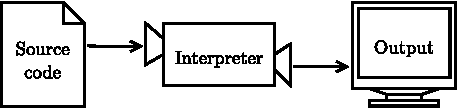
\includegraphics{figs/interpreter.pdf}
\caption{How interpreted languages are executed.}
\label{fig.interpreter}
\end{center}
\end{figure}

\index{compile}
\index{source code}
\index{object code}
\index{executable}

In contrast, a {\bf compiler} reads the entire program and translates it completely before the program starts running.
In this context, the high-level program is called the {\bf source code}, and the translated program is called the {\bf object code} or the {\bf executable}.
Once a program is compiled, you can execute it repeatedly without further translation.
As a result, compiled programs often run faster than interpreted programs.
% Figure 1.2 shows the structure of a compiler.

\index{byte code}
\index{virtual machine}
\index{JVM}

Java is {\em both} compiled and interpreted.
Instead of translating programs directly into machine language, the Java compiler generates {\bf byte code}.
Similar to machine language, byte code is easy and fast to interpret.
But it is also portable, so it is possible to compile a Java program on one machine, transfer the byte code to another machine, and run the byte code on the other machine.
The interpreter that runs byte code is called a ``Java Virtual Machine'' (JVM).
%This ability is an advantage of Java over some other high-level languages.

\begin{figure}[!ht]
\begin{center}
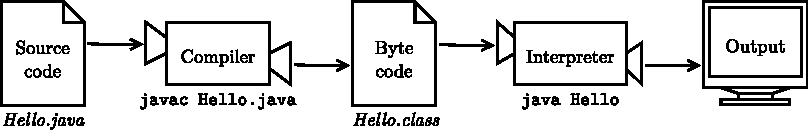
\includegraphics{figs/compiler.pdf}
\caption{The process of compiling and running a Java program.}
\label{fig.compiler}
\end{center}
\end{figure}

Figure~\ref{fig.compiler} shows the steps of this process.
Although it might seem complicated, these steps are automated for you in most program development environments.
Usually you only have to press a button or type a single command to compile and run your program.
On the other hand, it is important to know what steps are happening in the background, so if something goes wrong you can figure out what it is.


\section{The hello world program}
\label{hello}

\index{hello world}

Traditionally, the first program you write when learning a new programming language is called the hello world program.
All it does is display the words ``Hello, World!''\ on the screen.
In Java, it looks like this:

% NOTE(ABD): I changed a lot of ``print'' to ``display'', partly to be
% more precise, but also to reduce the number of times ``print'' appears,
% which is a lot!

% height = 130 + 15 * num_lines
\begin{trinket}[235]{Hello.java}
public class Hello {

    public static void main(String[] args) {
        // generate some simple output
        System.out.println("Hello, World!");
    }
}
\end{trinket}

When this program runs it displays:

\begin{stdout}
Hello, World!
\end{stdout}

Notice that the output does not include the quotation marks.

%\index{public}
%\index{static}
%The word \java{public} means the code can be accessed from other source files.
%The word \java{static} means that memory is allocated for the program in advance.

%Unfortunately, this simple example uses language features (like \java{public} and \java{static}) that are hard to explain.
%In fact, we won't be able to explain all of them for several more chapters.
%But we can start with the structure.

\index{class!definition}
\index{method!definition}
\index{statement}
\index{print statement}

Java programs are made up of {\em class} and {\em method} definitions, and methods are made up of {\em statements}.
A {\bf statement} is a line of code that performs a basic operation.
In the hello world program, this line is a {\bf print statement} that displays a message on the screen:

\begin{code}
System.out.println("Hello, World!");
\end{code}

\index{println}
\index{semicolon}

\java{System.out.println} displays results on the screen; the name \java{println} stands for ``print line''.
Confusingly, {\em print} can mean both ``display on the screen'' and ``send to the printer''.
In this book, we'll try to say ``display'' when we mean output to the screen.
Like most statements, the print statement ends with a semicolon (\java{;}).

\index{case-sensitive}

Java is ``case-sensitive'', which means that uppercase and lowercase are not the same.
In this example, \java{System} has to begin with an uppercase letter; \java{system} and \java{SYSTEM} won't work.

\index{method}

A {\bf method} is a named sequence of statements.
This program defines one method named \java{main}:

\begin{code}
public static void main(String[] args)
\end{code}

\index{main}

The name and format of \java{main} is special: when the program runs, it starts at the first statement in \java{main} and ends when it finishes the last statement.
Later, we will see programs that define more than one method.

\index{class}

A {\bf class} is a collection of methods.
This program defines a class named \java{Hello}.
You can give a class any name you like, but it is conventional to start with a capital letter.
The name of the class has to match the name of the file it is in, so this class has to be in a file named {\tt Hello.java}.

Java uses squiggly braces (\{ and \}) to group things together.
In {\tt Hello.java}, the outermost braces contain the class definition, and the inner braces contain the method definition.

\index{comment!inline}
\index{statement!comment}

The line that begins with two slashes (\java{//}) is a {\bf comment}, which is a bit of English text that explains the code.
When the compiler sees \java{//}, it ignores everything from there until the end of the line.
Comments have no effect on the execution of the program, but they make it easier for other programmers (and your future self) to understand what you meant to do.


\section{Displaying strings}

You can put as many statements as you like in \java{main}.
For example, to display more than one line of output:

\begin{trinket}[250]{Hello.java}
public class Hello {

    public static void main(String[] args) {
        // generate some simple output
        System.out.println("Hello, World!");  // first line
        System.out.println("How are you?");   // another line
    }
}
\end{trinket}

As this example shows, you can put comments at the end of a line as well as on lines all by themselves.

\index{quote mark}
\index{string}
\index{type!String}
\index{char}

Phrases that appear in quotation marks are called {\bf strings}, because they contain a sequence of ``characters'' strung together.
Characters can be letters, numbers, punctuation marks, symbols, spaces, tabs, etc.

\index{newline}
\index{print}
\index{statement!print}

\java{System.out.println} appends a special character, called a {\bf newline}, that moves to the beginning of the next line.
If you don't want a newline at the end, you can use \java{print} instead of \java{println}:

\begin{trinket}[235]{Goodbye.java}
public class Goodbye {

    public static void main(String[] args) {
        System.out.print("Goodbye, ");
        System.out.println("cruel world");
    }
}
\end{trinket}

\label{goodbye}

In this example, the first statement does not add a newline, so the output appears on a single line as {\tt Goodbye, cruel world}.
Notice that there is a space at the end of the first string, which appears in the output.


\section{Escape sequences}

It is possible to display multiple lines of output in just one line of code.
You just have to tell Java where to put the line breaks.

\begin{trinket}[220]{Hello.java}
public class Hello {

    public static void main(String[] args) {
        System.out.print("Hello!\nHow are you doing?\n");
    }
}
\end{trinket}

The output is two lines, each ending with a newline character:

\begin{stdout}
Hello!
How are you doing?
\end{stdout}

\index{escape sequence}

The \verb"\n" is an {\bf escape sequence}, which is a sequence of characters that represents a special character.
The backslash allows you to ``escape'' the string's literal interpretation.
Notice there is no space between \verb"\n" and \verb"How".
If you add a space there, there will be a space at the beginning of the second line.

\begin{table}[!ht]
\begin{center}
\begin{tabular}{|c|c|}
\hline
\verb"\n" & newline \\
\hline
\verb"\t" & tab \\
\hline
\verb'\"' & double quote \\
\hline
\verb"\\" & backslash \\
\hline
\end{tabular}
\caption{Common escape sequences}
\end{center}
\end{table}

\index{quote mark}

Another common use of escape sequences is to have quotation marks inside of strings.
Since double quotes indicate the beginning and end of strings, you need to escape them with a backslash.

\begin{code}
System.out.println("She said \"Hello!\" to me.");
\end{code}

The result is:

\begin{stdout}
She said "Hello!" to me.
\end{stdout}


\section{Formatting code}
\label{formatting}

In Java programs, some spaces are required.
For example, you need at least one space between words, so this program is not legal:

\begin{code}
publicclassGoodbye{

    publicstaticvoidmain(String[] args) {
        System.out.print("Goodbye, ");
        System.out.println("cruel world");
    }
}
\end{code}

But most other spaces are optional.
For example, this program is legal:

\begin{trinket}[220]{Goodbye.java}
public class Goodbye {
public static void main(String[] args) {
System.out.print("Goodbye, ");
System.out.println("cruel world");
}
}
\end{trinket}

The newlines are optional, too.
So we could just write:

\begin{trinket}[175]{Goodbye.java}
public class Goodbye { public static void main(String[] args)
{ System.out.print("Goodbye, "); System.out.println
("cruel world");}}
\end{trinket}

It still works, but the program is getting harder and harder to read.
Newlines and spaces are important for organizing your program visually, making it easier to understand the program and find errors when they occur.

Many editors will automatically format source code with consistent indenting and line breaks.
For example, in DrJava (see Appendix~\ref{development}) you can indent the code by selecting all text ({\sf Ctrl+A}) and pressing the {\sf Tab} key.


%\section{Style guidelines}

%\index{whitespace}
%
%As we saw in Section~\ref{formatting}, the compiler generally ignores spaces, tabs, and newlines.
%These characters, which are called {\bf whitespace}, affect the format of the code, but they don't affect its behavior.

%You have a lot of freedom in how you arrange your code.
%However with that freedom comes responsibility, both to yourself (when you look at the code in the future) and others who will be reading, understanding, and debugging it.

\index{Google style}

Organizations that do a lot of software development usually have strict guidelines on how to format source code.
For example, Google publishes its Java coding standards for use in open-source projects: \url{http://google.github.io/styleguide/javaguide.html}.
%It is easier to understand a large codebase when all the source code is formatted consistently.
%Plus following style guidelines helps you to avoid common programming mistakes that are difficult to debug.

You might not understand these guidelines now, because they refer to language features we haven't yet seen.
But you might want to refer back to them periodically as you read this book.

%In the meantime, there are many software tools that help programmers find and correct style issues.
%One of the most popular is Checkstyle, which enforces most of Google's guidelines.
%Instructions for downloading and running Checkstyle are in Appendix~\ref{checkstyle}.


\section{Debugging code}
\label{sec:examples}

It is a good idea to read this book in front of a computer so you can try out the examples as you go.
You can run many of the examples directly in DrJava's Interactions Pane (see Appendix~\ref{development}).
But if you put the code in a source file, it will be easier to try out variations.
%For more information on working with DrJava, see Appendix~\ref{development}.

\index{error!message}

Whenever you are experimenting with a new feature, you should also try to make mistakes.
For example, in the hello world program, what happens if you leave out one of the quotation marks?
What if you leave out both?
What if you spell \java{println} wrong?
These kinds of experiments help you remember what you read.
They also help with debugging, because you learn what the error messages mean.
It is better to make mistakes now and on purpose than later on and accidentally.

\index{experimental debugging}
\index{debugging!experimental}

%\index{Holmes, Sherlock}
%\index{Doyle, Arthur Conan}

Debugging is like an experimental science: once you have an idea about what is going wrong, you modify your program and try again.
If your hypothesis was correct, then you can predict the result of the modification, and you take a step closer to a working program.
If your hypothesis was wrong, you have to come up with a new one.
%As Sherlock Holmes pointed out, ``When you have eliminated the impossible, whatever remains, however improbable, must be the truth.''
%(A.~Conan Doyle, {\em The Sign of Four}.)

Programming and debugging should go hand in hand.
Don't just write a bunch of code and then perform trial and error debugging until it all works.
Instead, start with a program that does {\em something} and make small modifications, debugging them as you go, until the program does what you want.
That way you will always have a working program, and it will be easier to isolate errors.

\index{Linux}
\index{Torvalds, Linus}
\index{Greenfield, Larry}

A great example of this principle is the Linux operating system, which contains millions of lines of code.
It started out as a simple program Linus Torvalds used to explore the Intel 80386 chip.
According to Larry Greenfield in {\it The Linux Users' Guide}, ``One of Linus's earlier projects was a program that would switch between printing AAAA and BBBB.
This later evolved to Linux.''

%Later chapters will make more suggestions about debugging and other programming practices.

Finally, programming sometimes brings out strong emotions.
If you are struggling with a difficult bug, you might feel angry, despondent, or embarrassed.
Remember that you are not alone, and most if not all programmers have had similar experiences.
Don't hesitate to reach out to a friend and ask questions!


\section{Vocabulary}

Throughout the book, we try to define each term the first time we use it.
At the end of each chapter, we include the new terms and their definitions in order of appearance.
If you spend some time learning this vocabulary, you will have an easier time reading the following chapters.

\begin{description}

\term{problem solving}
The process of formulating a problem, finding a solution, and expressing the solution.

\term{program}
A sequence of instructions that specifies how to perform tasks on a computer.

\term{programming}
The application of problem solving to creating executable computer programs.

\term{computer science}
The scientific and practical approach to computation and its applications.

\term{algorithm}
A procedure or formula for solving a problem, with or without a computer.

\term{bug}
An error in a program.

\term{debugging}
The process of finding and removing errors.

\term{high-level language}
A programming language that is designed to be easy for humans to read and write.

\term{low-level language}
A programming language that is designed to be easy for a computer to run.
Also called ``machine language'' or ``assembly language''.

\term{portable}
The ability of a program to run on more than one kind of computer.

\term{interpret}
To run a program in a high-level language by translating it one line at a time and immediately executing the corresponding instructions.

\term{compile}
To translate a program in a high-level language into a low-level language, all at once, in preparation for later execution.

\term{source code}
A program in a high-level language, before being compiled.

\term{object code}
The output of the compiler, after translating the program.

\term{executable}
Another name for object code that is ready to run on specific hardware.

\term{byte code}
A special kind of object code used for Java programs.
Byte code is similar to a low-level language, but it is portable like a high-level language.

\term{statement}
Part of a program that specifies one step of an algorithm.

\term{print statement}
A statement that causes output to be displayed on the screen.

\term{method}
A named sequence of statements.

\term{class}
For now, a collection of related methods.
(We will see later that there is more to it.)

\term{comment}
A part of a program that contains information about the program but has no effect when the program runs.

\term{string}
A sequence of characters; the primary data type for text.

\term{newline}
A special character signifying the end of a line of text.
Also known as line ending, end of line (EOL), or line break.

\term{escape sequence}
A sequence of code that represents a special character when used inside a string.

%\term{whitespace}
%Newlines, tab characters, and other spaces in a source program.
%Whitespace characters are used to separate words, but other than that, they don't affect the behavior of the program.

\end{description}


\section{Exercises}

At the end of each chapter, we include exercises you can do with the things you've learned.
We encourage you to at least attempt every problem.
You can't learn to program only by reading about it; you have to practice.

Before you can compile and run Java programs, you might have to download and install a few tools.
There are many good options, but we recommend DrJava, which is an ``integrated development environment'' (IDE) well suited for beginners.
Instructions for getting started are in Appendix~\ref{drjava}.

The code for this chapter is in the {\tt ch01} directory of {\tt ThinkJavaCode}.
See page~\pageref{code} for instructions on how to download the repository.
Before you start the exercises, we recommend that you compile and run the examples.


\begin{exercise}

Computer scientists have the annoying habit of using common English words to mean something other than their common English meaning.
For example, in English, statements and comments are the same thing, but in programs they are different.

\begin{enumerate}
\item In computer jargon, what's the difference between a statement and a comment?
\item What does it mean to say that a program is portable?
\item In common English, what does the word compile mean?
\item What is an executable? Why is that word used as a noun?
\end{enumerate}

The glossary at the end of each chapter is intended to highlight words and phrases that have special meanings in computer science.
When you see familiar words, don't assume that you know what they mean!

\end{exercise}


\begin{exercise}

Before you do anything else, find out how to compile and run a Java program.
Some environments provide sample programs similar to the example in Section~\ref{hello}.

\begin{enumerate}
\item Type in the hello world program, then compile and run it.

\item Add a print statement that displays a second message after the ``Hello, World!''.
Say something witty like, ``How are you?''
Compile and run the program again.

\item Add a comment to the program (anywhere), recompile, and run it again.
The new comment should not affect the result.
\end{enumerate}

This exercise may seem trivial, but it is the starting place for many of the programs we will work with.
To debug with confidence, you will need to have confidence in your programming environment.

In some environments, it is easy to lose track of which program is executing.
You might find yourself trying to debug one program while you are accidentally running another.
Adding (and changing) print statements is a simple way to be sure that the program you are looking at is the program you are running.

\end{exercise}


\begin{exercise}

It is a good idea to commit as many errors as you can think of, so that you see what error messages the compiler produces.
Sometimes the compiler tells you exactly what is wrong, and all you have to do is fix it.
But sometimes the error messages are misleading.
Over time you will develop a sense for when you can trust the compiler and when you have to figure things out yourself.

Starting with the hello world program, try out each of the following errors.
After you make each change, compile the program, read the error message (if there is one), and then fix the error.

\begin{enumerate}
\item Remove one of the open squiggly braces.
\item Remove one of the close squiggly braces.
\item Instead of \java{main}, write \java{mian}.
\item Remove the word \java{static}.
\item Remove the word \java{public}.
\item Remove the word \java{System}.
\item Replace \java{println} with \java{Println}.
\item Replace \java{println} with \java{print}.
\item Delete one of the parentheses.
Add an extra one.
\end{enumerate}

\end{exercise}


\chapter{Variables and operators}

This chapter describes how to write statements using {\em variables}, which store values like numbers and words, and {\em operators}, which are symbols that perform a computation.
We also explain three kinds of programming errors and offer additional debugging advice.
%Understanding what can go wrong will help you get it right.
%Finally we discuss the rules of code style, which helps make programs easier to read and debug.

To run the examples in this chapter, you will need to create a new Java class with a \java{main} method (see Section~\ref{hello}).
We often omit the class and method definitions to keep the examples concise.


\section{Declaring variables}

%NOTE: in response to review comments, I am cleaning up the use of
% ``memory''.  I would like to avoid talking about hardware, or being
% specific about where values are stored.  The addresses that appear
% as object IDs are actually virtual addresses; the values themselves
% might be in RAM or on HDD.  But we really don't want to get into
% that.  I'd rather offer the abstract model that a variable indicates
% a location that contains a value.

\index{variable}
\index{value}

One of the most powerful features of a programming language is the ability to define and manipulate {\bf variables}.
A variable is a named location in memory that stores a {\bf value}.
Values may be numbers, text, images, sounds, and other types of data.
%They can be printed, and as we'll see later, operated on.
To store a value, you first have to declare a variable.
%Since the values we want to store are text, we declare that the new variable is a string:

\begin{code}
String message;
\end{code}

\index{declaration}
\index{statement!declaration}
\index{type!int}
\index{type!char}
\index{type!String}

This statement is called a {\bf declaration}, because it declares that the variable named \java{message} has the type \java{String}.
Each variable has a {\bf type} that determines what kind of values it can store.
For example, the \java{int} type can store integers, and the \java{char} type can store characters.

Some types begin with a capital letter and some with lowercase.
We will learn the significance of this distinction later, but for now you should take care to get it right.
There is no such type as \java{Int} or \java{string}.
%, and the compiler will complain if you make one up.

To declare an integer variable named \java{x}, you simply type:

\begin{code}
int x;
\end{code}

Note that \java{x} is an arbitrary name for the variable.
In general, you should use names that indicate what the variables mean.
%For example, if you saw these declarations, you could probably guess what values would be stored:

\begin{code}
String firstName;
String lastName;
int hour, minute;
\end{code}

\index{semicolon}

This example declares two variables with type \java{String} and two with type \java{int}.
The last line shows how to declare multiple variables with the same type: \java{hour} and \java{minute} are both integers.
Note that each declaration statement ends with a semicolon (\java{;}).

\index{case-sensitive}

Variable names usually begin with a lowercase letter, in contrast to class names (like \java{Hello}) that start with a capital letter.
When a variable name contains more than one word (like \java{firstName}), it is conventional to capitalize the first letter of each subsequent word.
Variable names are case-sensitive, so \java{firstName} is not the same as \java{firstname} or \java{FirstName}.

\index{keyword}

You can use any name you want for a variable.
But there are about 50 reserved words, called {\bf keywords}, that you are not allowed to use as variable names.
These words include \java{public}, \java{class}, \java{static}, \java{void}, and \java{int}, which are used by the compiler to analyze the structure of the program.

You can find the complete list of keywords at \url{http://docs.oracle.com/javase/tutorial/java/nutsandbolts/_keywords.html}, but you don't have to memorize them.
Most programming editors provide ``syntax highlighting'', which makes different parts of the program appear in different colors.
%For example, keywords are often blue, strings red, comments green, and other code black.
%If you type a variable name and it turns blue, watch out!


\section{Assigning variables}

\index{assignment}
\index{statement!assignment}

Now that we have declared some variables, we can use them to store values.
We do that with an {\bf assignment} statement.

\begin{code}
message = "Hello!";  // give message the value "Hello!"
hour = 11;           // assign the value 11 to hour
minute = 59;         // set minute to 59
\end{code}

This example shows three assignments, and the comments illustrate different ways people sometimes talk about assignment statements.
The vocabulary can be confusing here, but the idea is straightforward:

\begin{itemize}
\item When you declare a variable, you create a named storage location.
\item When you make an assignment to a variable, you update its value.
\end{itemize}

As a general rule, a variable has to have the same type as the value you assign to it.
For example, you cannot store a string in \java{minute} or an integer in \java{message}.
We will see some examples that seem to break this rule, but we'll get to that later.

%On the other hand, that rule can be confusing.
%There are many ways that you can convert values from one type to another, and Java sometimes converts things automatically.
%For now you should remember the general rule, and we'll talk about exceptions later.

A common source of confusion is that some strings {\em look} like integers, but they are not.
For example, \java{message} can contain the string \java{"123"}, which is made up of the characters \java{'1'}, \java{'2'}, and \java{'3'}.
But that is not the same thing as the integer \java{123}.

\begin{code}
message = "123";     // legal
message = 123;       // not legal
\end{code}

\index{initialize}

Variables must be {\bf initialized} (assigned for the first time) before they can be used.
You can declare a variable and then assign a value later, as in the previous example.
You can also declare and initialize on the same line:

\begin{code}
String message = "Hello!";
int hour = 11;
int minute = 59;
\end{code}

%You can make more than one assignment to the same variable.
%For example:
%
%\begin{code}
%int i = 1;
%i = 2;
%\end{code}
%
%\index{update}
%
%The first line initializes \java{i} to 1.
%The second line changes its value to \java{2}.
%In this example, there is no reason to make two assignments, but in many programs it is useful to reassign, or {\bf update}, variables.


\section{Memory diagrams}
\label{state}

Because Java uses the \java{=} symbol for assignment, it is tempting to interpret the statement \java{a = b} as a statement of equality.
It is not!

Equality is commutative, and assignment is not.
For example, in mathematics if $a = 7$ then $7 = a$.
In Java \java{a = 7;} is a legal assignment statement, but \java{7 = a;} is not.
The left side of an assignment statement has to be a variable name (storage location).

Also, in mathematics, a statement of equality is true for all time.
If $a = b$ now, $a$ is always equal to $b$.
In Java, an assignment statement can make two variables equal, but they don't have to stay that way.

\begin{code}
int a = 5;
int b = a;     // a and b are now equal
a = 3;         // a and b are no longer equal
\end{code}

The third line changes the value of \java{a}, but it does not change the value of \java{b}, so they are no longer equal.

\index{state}

Taken together, the variables in a program and their current values make up the program's {\bf state}.
Figure~\ref{fig.state} shows the state of the program after these assignment statements run.

\begin{figure}[!ht]
\begin{center}
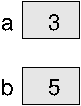
\includegraphics{figs/state.pdf}
\caption{Memory diagram of the variables \java{a} and \java{b}.}
\label{fig.state}
\end{center}
\end{figure}

\index{memory diagram}
\index{diagram!memory}

Diagrams like this one that show the state of the program are called {\bf memory diagrams}.
Each variable is represented with a box showing the name of the variable on the outside and the value inside.
As the program runs, the state of memory changes, so memory diagrams only show a particular point in time.


\section{Printing variables}
\label{sec:printvar}

You can display the current value of a variable using \java{print} or \java{println}.
The following statements declare a variable named \java{firstLine}, assign it the value \java{"Hello, again!"}, and display that value.

\begin{code}
String firstLine = "Hello, again!";
System.out.println(firstLine);
\end{code}

%Assuming this code fragment is inside a method that is inside a class, the output is:
%
%\begin{stdout}
%Hello, again!
%\end{stdout}

When we talk about displaying a variable, we generally mean the {\em value} of the variable.
To display the {\em name} of a variable, you have to put it in quotes.
%For example: \java{System.out.println("firstLine");}

\begin{code}
System.out.print("The value of firstLine is ");
System.out.println(firstLine);
\end{code}

For this example, the output is:

\begin{stdout}
The value of firstLine is Hello, again!
\end{stdout}

Conveniently, the code for displaying a variable is the same regardless of its type.
For example:

\begin{code}
int hour = 11;
int minute = 59;
System.out.print("The current time is ");
System.out.print(hour);
System.out.print(":");
System.out.print(minute);
System.out.println(".");
\end{code}

The output of this program is:

\begin{stdout}
The current time is 11:59.
\end{stdout}

To output multiple values on the same line, it's common to use several \java{print} statements followed by \java{println} at the end.
But don't forget the \java{println}!
On many computers, the output from \java{print} is stored without being displayed until \java{println} is run; then the entire line is displayed at once.
If you omit the \java{println}, the program might display the stored output at unexpected times or even terminate without displaying anything.


\section{Arithmetic operators}
\label{sec:arithops}

%Recall that Java programs are organized into {\em classes}, each of which has one or more {\em methods}, each of which has one or more {\em statements}.
%Most statements consist of one or more {\bf expressions}.

\index{operator}
\index{addition!integer}

{\bf Operators} are symbols that represent simple computations.
%Most operators in Java do what you expect them to do, since they are common mathematical symbols.
For example, the addition operator is \java{+}, subtraction is \java{-}, multiplication is \java{*}, and division is \java{/}.
%Variables are replaced with their values before the computation is performed.

The following program converts a time of day to minutes:

\begin{code}
int hour = 11;
int minute = 59;
System.out.print("Number of minutes since midnight: ");
System.out.println(hour * 60 + minute);
\end{code}

The output is:

\begin{stdout}
Number of minutes since midnight: 719
\end{stdout}

\index{expression}
\index{operand}

In this program, \java{hour * 60 + minute} is an {\bf expression}, which represents a single value to be computed (\java{719}).
When the program runs, each variable is replaced by its current value, and then the operators are applied.
The values that operators work with are called {\bf operands}.

Expressions are generally a combination of numbers, variables, and operators.
When compiled and executed, they become a single value.
For example, the expression \java{1 + 1} has the value \java{2}.
In the expression \java{hour - 1}, Java replaces the variable with its value, yielding \java{11 - 1}, which has the value \java{10}.

In the expression \java{hour * 60 + minute}, both variables get replaced, yielding \java{11 * 60 + 59}.
The multiplication happens first, yielding \java{660 + 59}.
Then the addition yields \java{719}.

Addition, subtraction, and multiplication all do what you expect, but you might be surprised by division.
For example, the following fragment tries to compute the fraction of an hour that has elapsed:%, but it has a logic error:

\begin{code}
System.out.print("Fraction of the hour that has passed: ");
System.out.println(minute / 60);
\end{code}

The output is:

\begin{stdout}
Fraction of the hour that has passed: 0
\end{stdout}

\index{division!integer}
\index{integer division}
\index{arithmetic!integer}

This result often confuses people.
The value of \java{minute} is 59, and 59 divided by 60 should be 0.98333, not 0.
The problem is that Java performs ``integer division'' when the operands are integers.
By design, integer division always rounds toward zero, even in cases like this one where the next integer is close.

As an alternative, we can calculate a percentage rather than a fraction:

\begin{code}
System.out.print("Percent of the hour that has passed: ");
System.out.println(minute * 100 / 60);
\end{code}

The new output is:

\begin{stdout}
Percent of the hour that has passed: 98
\end{stdout}

Again the result is rounded down, but at least now it's approximately correct.
%To get a more precise answer, we can use a different type of variable that can store fractional values.


\section{Floating-point numbers}

\index{floating-point}
\index{double}
\index{type!double}

A more general solution is to use {\bf floating-point} numbers, which can represent fractions as well as integers.
%As the name implies, the decimal point floats around (i.e., you can have as many decimal places as you want).
In Java, the default floating-point type is called \java{double}, which is short for double-precision.
You can create \java{double} variables and assign values to them the same way we did for the other types:

\begin{code}
double pi;
pi = 3.14159;
\end{code}

Java performs ``floating-point division'' when one or more operands are \java{double} values.
So we can solve the problem we saw in the previous section:

\begin{code}
double minute = 59.0;
System.out.print("Fraction of the hour that has passed: ");
System.out.println(minute / 60.0);
\end{code}

The output is:

\begin{stdout}
Fraction of the hour that has passed: 0.9833333333333333
\end{stdout}

Although floating-point numbers are useful, they can be a source of confusion.
For example, Java distinguishes the integer value \java{1} from the floating-point value \java{1.0}, even though they seem to be the same number.
They belong to different data types, and strictly speaking, you are not allowed to make assignments between types.

The following is illegal because the variable on the left is an \java{int} and the value on the right is a \java{double}:

\begin{code}
int x = 1.1;  // compiler error
\end{code}

It is easy to forget this rule, because in many cases Java {\em automatically} converts from one type to another:

\begin{code}
double y = 1;  // legal, but bad style
\end{code}

The preceding example should be illegal, but Java allows it by converting the \java{int} value \java{1} to the \java{double} value \java{1.0} automatically.
This leniency is convenient, but it often causes problems for beginners.
For example:

\begin{code}
double y = 1 / 3;  // common mistake
\end{code}

\index{division!integer}
\index{integer division}
\index{arithmetic!integer}

You might expect the variable \java{y} to get the value \java{0.333333}, which is a legal floating-point value.
But instead it gets the value \java{0.0}.
The expression on the right divides two integers, so Java does integer division, which yields the \java{int} value \java{0}.
Converted to \java{double}, the value assigned to \java{y} is \java{0.0}.

One way to solve this problem (once you figure out the bug) is to make the right-hand side a floating-point expression.
The following sets \java{y} to \java{0.333333}, as expected:

\begin{code}
double y = 1.0 / 3.0;  // correct
\end{code}

As a matter of style, you should always assign floating-point values to floating-point variables.
The compiler won't make you do it, but you never know when a simple mistake will come back and haunt you.


\section{Rounding errors}

%The operations we have seen so far -- addition, subtraction, multiplication, and division -- also work on floating-point values, although you might be interested to know that the underlying mechanism is completely different.
%In fact, most processors have special circuitry just for performing floating-point operations.

Most floating-point numbers are only {\em approximately} correct.
Some numbers, like reasonably-sized integers, can be represented exactly.
But repeating fractions, like $1/3$, and irrational numbers, like $\pi$, cannot.
To represent these numbers, computers have to round off to the nearest floating-point number.

%Notwithstanding, there is a fundamental flaw with floating-point arithmetic.
%In mathematics, there is an infinite number of real numbers.
%But computer processors are finite; they cannot represent {\em every} possible floating-point number.
%Even with double-precision, you will frequently run into problems.

\index{rounding error}
\index{arithmetic!floating-point}

The difference between the number we want and the floating-point number we get is called {\bf rounding error}.
For example, the following two statements should be equivalent:

\begin{code}
System.out.println(0.1 * 10);
System.out.println(0.1 + 0.1 + 0.1 + 0.1 + 0.1
                 + 0.1 + 0.1 + 0.1 + 0.1 + 0.1);
\end{code}

But on many machines, the output is:

\begin{stdout}
1.0
0.9999999999999999
\end{stdout}

The problem is that \java{0.1}, which is a terminating fraction in decimal, is a repeating fraction in binary.
So its floating-point representation is only approximate.
When we add up the approximations, the rounding errors accumulate.

For many applications, like computer graphics, encryption, statistical analysis, and multimedia rendering, floating-point arithmetic has benefits that outweigh the costs.
But if you need {\em absolute} precision, use integers instead.
For example, consider a bank account with a balance of \$123.45:

\begin{code}
double balance = 123.45;  // potential rounding error
\end{code}

In this example, balances will become inaccurate over time as the variable is used in arithmetic operations like deposits and withdrawals.
The result would be angry customers and potential lawsuits.
You can avoid the problem by representing the balance as an integer:

\begin{code}
int balance = 12345;      // total number of cents
\end{code}

\index{type!long}

This solution works as long as the number of cents doesn't exceed the largest integer, which is about 2 billion.
%If necessary you can use \java{long} instead, which has a max value of $2^{63}-1$ (about 92 quadrillion dollars).
%Hopefully nobody will ever need that much money!


\section{Operators for strings}

\index{string!operator}
\index{operator!string}

In general, you cannot perform mathematical operations on strings, even if the strings look like numbers.
The following expressions are illegal:

\begin{code}
"Hello" - 1     "World" / 123     "Hello" * "World"
\end{code}

\index{concatenate}
\index{addition!string}

The \java{+} operator works with strings, but it might not do what you expect.
For strings, the \java{+} operator performs {\bf concatenation}, which means joining end-to-end.
So \java{"Hello, " + "World!"} yields the string \java{"Hello, World!"}.

Likewise if you have a variable called \java{name} that has type \java{String}, the expression \java{"Hello, " + name} appends the value of \java{name} to the hello string, which creates a personalized greeting.

Since addition is defined for both numbers and strings, Java performs automatic conversions you may not expect:

\begin{code}
System.out.println(1 + 2 + "Hello");
// the output is 3Hello

System.out.println("Hello" + 1 + 2);
// the output is Hello12
\end{code}

Java executes these operations from left to right.
In the first line, \java{1 + 2} is \java{3}, and \java{3 + "Hello"} is \java{"3Hello"}.
But in the second line, \java{"Hello" + 1} is \java{"Hello1"}, and \java{"Hello1" + 2} is \java{"Hello12"}.


%\section{Order of operations}

\index{order of operations}
\index{precedence}

When more than one operator appears in an expression, they are evaluated according to the {\bf order of operations}.
Generally speaking, Java evaluates operators from left to right (as we saw in the previous section).
But for numeric operators, Java follows mathematical conventions:

\begin{itemize}

\item Multiplication and division take ``precedence'' over addition and subtraction, which means they happen first.
So \java{1 + 2 * 3} yields 7, not 9, and \java{2 + 4 / 2} yields 4, not 3.

\item If the operators have the same precedence, they are evaluated from left to right.
So in the expression \java{minute * 100 / 60}, the multiplication happens first; if the value of \java{minute} is 59, we get \java{5900 / 60}, which yields \java{98}.
If these same operations had gone from right to left, the result would have been \java{59 * 1}, which is incorrect.

\item Any time you want to override the order of operations (or you are not sure what it is) you can use parentheses.
Expressions in parentheses are evaluated first, so \java{(1 + 2) * 3} is 9.
You can also use parentheses to make an expression easier to read, as in \java{(minute * 100) / 60}, even though it doesn't change the result.

\end{itemize}

See the Java tutorials for a complete table of operator precedence: \url{https://docs.oracle.com/javase/tutorial/java/nutsandbolts/operators.html}.
If the order of operations is not obvious when looking at an expression, you can always add parentheses to make it more clear.
But over time, you should internalize these kinds of details about the Java language.


\section{Compiler error messages}

\index{error!message}

Three kinds of errors can occur in a program: compile-time errors, run-time errors, and logic errors.
It is useful to distinguish among them in order to track them down more quickly.

\index{compile-time error}
\index{error!compile-time}

{\bf Compile-time} errors occur when you violate the rules of the Java language.
For example, parentheses and braces have to come in matching pairs.
So \java{(1 + 2)} is legal, but \java{8)} is not.
In the latter case, the program cannot be compiled, and the compiler displays an error.

\index{error!message}

Error messages from the compiler usually indicate where in the program the error occurred, and sometimes they can tell you exactly what the error is.
As an example, let's get back to the hello world program from Section~\ref{hello}.

\begin{trinket}[235]{Hello.java}
public class Hello {

    public static void main(String[] args) {
        // generate some simple output
        System.out.println("Hello, World!");
    }
}
\end{trinket}

\index{semicolon}

If you forget the semicolon at the end of the print statement, you might get an error message like this:

\begin{stdout}
File: Hello.java  [line: 5]
Error: ';' expected
\end{stdout}

That's pretty good: the location of the error is correct, and the error message tells you what's wrong.
But error messages are not always easy to understand.
Sometimes the compiler reports the place in the program where the error was {\em detected}, not where it actually occurred.
And sometimes the description of the problem is more confusing than helpful.

For example, if you forget the closing brace at the end of \java{main} (line 6), you might get a message like this:

\begin{stdout}
File: Hello.java  [line: 7]
Error: reached end of file while parsing
\end{stdout}

\index{parse}

There are two problems here.
First, the error message is written from the compiler's point of view, not yours.
{\bf Parsing} is the process of reading a program before translating; if the compiler gets to the end of the file while still parsing, that means something was omitted.
But the compiler doesn't know what.
It also doesn't know where.
The compiler discovers the error at the end of the program (line 7), but the missing brace should be on the previous line.

Error messages contain useful information, so you should make an effort to read and understand them.
But don't take them too literally.
During the first few weeks of your programming career, you will probably spend a lot of time tracking down compile-time errors.
As you gain experience, you will make fewer mistakes and find them more quickly.


\section{Other types of errors}
%\subsection{Run-time errors}

\index{run-time error}
\index{error!run-time}
\index{exception}

The second type of error is a {\bf run-time error}, so-called because it does not appear until after the program has started running.
In Java, these errors occur while the interpreter is executing byte code and something goes wrong.
These errors are also called ``exceptions'' because they usually indicate that something unexpected has happened.

Run-time errors are rare in the simple programs you will see in the first few chapters, so it might be a while before you encounter one.
When a run-time error occurs, the interpreter displays an error message that explains what happened and where.
For example, if you accidentally divide by zero you will get a message like:

\begin{small}
\begin{stdout}
Exception in thread "main" java.lang.ArithmeticException: / by zero
    at Hello.main(Hello.java:5)
\end{stdout}
\end{small}

\index{ArithmeticException}
\index{exception!Arithmetic}

Error messages are very useful for debugging.
The first line includes the name of the exception, \java{java.lang.ArithmeticException}, and a message that indicates more specifically what happened, \java{/ by zero}.
The next line shows the method where the error occurred; \java{Hello.main} indicates the method \java{main} in the class \java{Hello}.
It also reports the file where the method is defined, {\tt Hello.java}, and the line number where the error occurred, \java{5}.

Sometimes error messages contain additional information that doesn't make sense.
It can be a challenge to figure out where to find the useful parts without being overwhelmed by extraneous information.
Keep in mind that the line where the program crashed may not be the line that needs to be corrected.

%\subsection{Logic errors}

\index{logic error}
\index{error!logic}

The third type of error is a {\bf logic error}.
%{\bf Semantics} pertains to the meaning of a program; that is, what it does when it runs.
If your program has a logic error, it will compile and run without generating error messages, but it will not do the right thing.
Instead, it will do exactly what you told it to do.
For example, here is a version of the hello world program with a logic error:

\begin{trinket}[235]{Hello.java}
public class Hello {

    public static void main(String[] args) {
        System.out.println("Hello, ");
        System.out.println("World!");
    }
}
\end{trinket}

This program compiles and runs just fine, but the output is:

\begin{stdout}
Hello,
World!
\end{stdout}

Assuming that we wanted the output on one line, this is not correct.
The problem is that the first line uses \java{println}, when we probably meant to use \java{print} (see the ``goodbye world'' example of Section~\ref{goodbye}).

Identifying logic errors can be hard because you have to work backwards, looking at the output of the program, trying to figure out why it is doing the wrong thing, and how to make it do the right thing.
Usually the compiler and the interpreter can't help you, since they don't know what the right thing is.

%Now that you know about the three kinds of errors, take a quick look at Appendix~\ref{debugappendix} where we've collected some of our favorite debugging advice.
%It refers to language features we haven't yet covered, but it's good for you to know what's available when you need it.


\section{Vocabulary}

\begin{description}

\term{variable}
A named storage location for values.
All variables have a type, which is declared when the variable is created.

\term{value}
A number, string, or other data that can be stored in a variable.
Every value belongs to a type (for example, \java{int} or \java{String}).

\term{type}
Mathematically speaking, a set of values.
The type of a variable determines which values it can have.

\term{declaration}
A statement that creates a new variable and specifies its type.

\term{keyword}
A reserved word used by the compiler to analyze programs.
You cannot use keywords (like \java{public}, \java{class}, and \java{void}) as variable names.

\term{assignment}
A statement that gives a value to a variable.

\term{initialize}
To assign a variable for the first time.

%\term{update}
%An assignment that changes the value of a variable.

\term{state}
The variables in a program and their current values.

\term{memory diagram}
A graphical representation of the state of a program at a point in time.

\term{operator}
A symbol that represents a computation like addition, multiplication, or string concatenation.

\term{operand}
One of the values on which an operator operates.
Most operators in Java require two operands.

\term{expression}
A combination of variables, operators, and values that represents a single value.
Expressions also have types, as determined by their operators and operands.

\term{floating-point}
A data type that represents numbers with an integer part and a fractional part.
In Java, the default floating-point type is \java{double}.

\term{rounding error}
The difference between the number we want to represent and the nearest floating-point number.

\term{concatenate}
To join two values, often strings, end-to-end.

\term{order of operations}
The rules that determine in what order expressions are evaluated.
Also known as ``operator precedence''.

\term{compile-time error}
An error in the source code that makes it impossible to compile.
Also called a ``syntax error''.

\term{parse}
To analyze the structure of a program; what the compiler does first.

\term{run-time error}
An error in a program that makes it impossible to run to completion.
Also called an ``exception''.

\term{logic error}
An error in a program that makes it do something other than what the programmer intended.

\end{description}


\section{Exercises}

The code for this chapter is in the {\tt ch02} directory of {\tt ThinkJava2Code}.
See page~\pageref{code} for instructions on how to download the repository.
Before you start the exercises, we recommend that you compile and run the examples.

If you have not already read Appendix~\ref{interactions}, now might be a good time.
It describes the DrJava Interactions Pane, which is a useful way to develop and test short fragments of code without writing a complete class definition.


\begin{exercise}  %%V6 Ex2.1

If you are using this book in a class, you might enjoy this exercise.
Find a partner and play ``Stump the Chump'':

Start with a program that compiles and runs correctly.
One player looks away while the other player adds an error to the program.
Then the first player tries to find and fix the error.
You get two points if you find the error without compiling the program, one point if you find it using the compiler, and your opponent gets a point if you don't find it.

\end{exercise}


\begin{exercise}  %%V6 Ex2.2
\label{ex:date}

The point of this exercise is (1) to use string concatenation to display values with different types (\java{int} and \java{String}), and (2) to practice developing programs gradually by adding a few statements at a time.

\begin{enumerate}

\item Create a new program named {\tt Date.java}.
Copy or type in something like the hello world program and make sure you can compile and run it.

\item Following the example in Section~\ref{sec:printvar}, write a program that creates variables named \java{day}, \java{date}, \java{month}, and \java{year}.
The variable \java{day} will contain the day of the week (like Friday), and \java{date} will contain the day of the month (like the 13th).
%What type is each variable?
Assign values to those variables that represent today's date.

\item Display the value of each variable on a line by itself.
This is an intermediate step that is useful for checking that everything is working so far.
Compile and run your program before moving on.

\item Modify the program so that it displays the date in standard American format, for example: {\tt Thursday, July 16, 2015}.

\item Modify the program so it also displays the date in European format.
The final output should be:

\begin{stdout}
American format:
Thursday, July 16, 2015
European format:
Thursday 16 July 2015
\end{stdout}

%{\it Hint:} You should be able to copy, paste, and modify the code from Step 4 when completing Step 5.
\end{enumerate}

\end{exercise}


\begin{exercise}  %%V6 Ex2.3

The point of this exercise is to (1) use some of the arithmetic operators, and (2) start thinking about compound entities (like time of day) that are represented with multiple values.

\begin{enumerate}

\item Create a new program called {\tt Time.java}.
From now on, we won't remind you to start with a small, working program, but you should.

\item Following the example program in Section~\ref{sec:printvar}, create variables named \java{hour}, \java{minute}, and \java{second}.
Assign values that are roughly the current time.
Use a 24-hour clock so that at 2pm the value of \java{hour} is 14.

\item Make the program calculate and display the number of seconds since midnight.

\item Calculate and display the number of seconds remaining in the day.

\item Calculate and display the percentage of the day that has passed.
You might run into problems when computing percentages with integers, so consider using floating-point.

\item Change the values of \java{hour}, \java{minute}, and \java{second} to reflect the current time.
Then write code to compute the elapsed time since you started working on this exercise.

\end{enumerate}

{\it Hint:} You might want to use additional variables to hold values during the computation.
Variables that are used in a computation but never displayed are sometimes called ``intermediate'' or ``temporary'' variables.

\end{exercise}


\chapter{Input and output}

The programs we've looked at so far simply display messages, which doesn't really involve that much computation.
This chapter will show you how to read input from the keyboard, use that input to calculate a result, and then format that result for output.
%We will also look at some technical details about how operating systems work.


\section{The System class}

\index{class!System}

We have been using \java{System.out.println} for a while, but you might not have thought about what it means.
\java{System} is a class that provides methods related to the ``system'' or environment where programs run.
It also provides \java{System.out}, which is a special value that has additional methods (like \java{println}) for displaying output.

\index{System.out}

In fact, we can use \java{System.out.println} to display the value of \java{System.out}:

\begin{code}
System.out.println(System.out);
\end{code}

The result is:

\begin{stdout}
java.io.PrintStream@685d72cd
\end{stdout}

\index{package}

This output indicates that \java{System.out} is a \java{PrintStream}, which is defined in a package called \java{java.io}.
A {\bf package} is a collection of related classes; \java{java.io} contains classes for ``I/O'' which stands for input and output.

\index{address}
\index{hexadecimal}

The numbers and letters after the {\tt @} sign are the {\bf address} of \java{System.out}, represented as a hexadecimal (base 16) number.
The address of a value is its location in the computer's memory, which might be different on different computers.
In this example the address is \java{685d72cd}, but if you run the same code you will likely get something else.
%You can think of the address as a unique identifier for the object.

\index{library}

As shown in Figure~\ref{fig.system}, \java{System} is defined in a file called {\tt System.java}, and \java{PrintStream} is defined in {\tt PrintStream.java}.
These files are part of the Java {\bf library}, which is an extensive collection of classes that you can use in your programs.
The source code for these classes is usually included with the compiler (see Section~\ref{src.zip}).

\begin{figure}[!ht]
\begin{center}
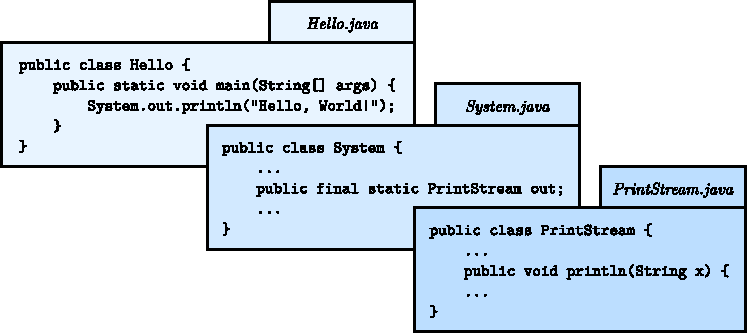
\includegraphics{figs/system.pdf}
\caption{\java{System.out.println} refers to the \java{out} variable of the \java{System} class, which is a \java{PrintStream} that provides a method called \java{println}.}
\label{fig.system}
\end{center}
\end{figure}


\section{The Scanner class}
\label{scanner}

\index{Scanner}
\index{class!Scanner}

%\index{byte}
%
%From the operating system's point of view, data from the keyboard arrives in a series of hardware control signals.
%The operating system translates these signals into a stream of {\bf bytes} (small integers), which in turn need to be translated into characters.
%\java{System.in} provides the means for reading one byte of input at a time, which is hardly useful for programs that would rather read in an entire word or line of input.

\index{System.in}

The \java{System} class also provides the special value \java{System.in}, which is an \java{InputStream} that has methods for reading input from the keyboard.
These methods are not convenient to use, but fortunately Java provides other classes that make it easy to handle common input tasks.

\index{class!utility}
\index{utility class}
\index{java.util}

For example, \java{Scanner} is a class that provides methods for inputting words, numbers, and other data.
\java{Scanner} is provided by \java{java.util}, which is a package that contains various ``utility classes''.
Before you can use \java{Scanner}, you have to import it like this:

\begin{code}
import java.util.Scanner;
\end{code}

\index{import statement}
\index{statement!import}

This {\bf import statement} tells the compiler that when you refer to \java{Scanner}, you mean the one defined in \java{java.util}.
Using an import statement is necessary because there might be another class named \java{Scanner} in another package.
%Using an import statement makes your code unambiguous.
Import statements can't be inside a class definition.
By convention, they are usually at the beginning of the file.

Next you have to initialize the \java{Scanner}.
This line declares a \java{Scanner} variable named \java{in} and creates a \java{Scanner} that reads input from \java{System.in}:
%We'll explain the \java{new} operator in more detail in Section~\ref{point}.

\begin{code}
Scanner in = new Scanner(System.in);
\end{code}

The \java{Scanner} class provides a method called \java{nextLine} that reads a line of input from the keyboard and returns a \java{String}.
The following example reads two lines and repeats them back to the user:

\index{Echo.java}

\begin{trinket}{Echo.java}
import java.util.Scanner;

public class Echo {

    public static void main(String[] args) {
        String line;
        Scanner in = new Scanner(System.in);

        System.out.print("Type something: ");
        line = in.nextLine();
        System.out.println("You said: " + line);

        System.out.print("Type something else: ");
        line = in.nextLine();
        System.out.println("You also said: " + line);
    }
}
\end{trinket}

If you omit the import statement at the top of the file, you will get a compiler error saying ``cannot find symbol''.
That means the compiler doesn't know where to find the definition for \java{Scanner}.

You might wonder why we can use the \java{System} class without importing it.
\java{System} belongs to the \java{java.lang} package, which is imported automatically.
According to the documentation, \java{java.lang} ``provides classes that are fundamental to the design of the Java programming language.''
The \java{String} class is also part of the \java{java.lang} package.


\section{Language elements}

\index{language!elements}

At this point, we have seen nearly all of the organizational units that make up Java programs.
Figure~\ref{fig.package} shows how these ``language elements'' are related.

\begin{figure}[!ht]
\begin{center}
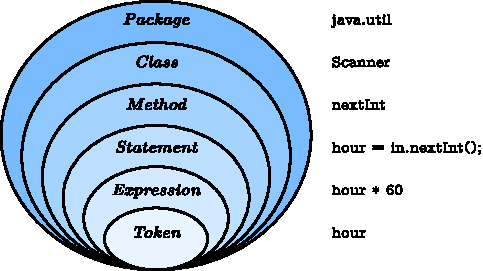
\includegraphics[width=4in]{figs/package.pdf}
\caption{Elements of the Java language, from largest to smallest.}
\label{fig.package}
\end{center}
\end{figure}

\index{token}

Java applications are typically organized into packages (like \java{java.io} and \java{java.util}) that include multiple classes (like \java{PrintStream} and \java{Scanner}).
Each class defines its own methods (like \java{println} and \java{nextLine}), and each method is a sequence of statements.

Each statement performs one or more computations, depending on how many expressions it has, and each expression represents a single value to compute.
For example, the assignment statement \java{hours = minutes / 60.0;} contains a single expression: \java{minutes / 60.0}.

{\bf Tokens} are the most basic elements of a program, including numbers, variable names, operators, keywords, parentheses, braces, and semicolons.
In the previous example, the tokens are \java{hours}, \java{=}, \java{minutes}, \java{/}, \java{60.0}, and \java{;} (spaces are ignored by the compiler).

%\index{syntax}
%\index{semantics}

Knowing this terminology is helpful, because error messages often say things like ``not a statement'' or ``illegal start of expression'' or ``unexpected token''.
Comparing Java to English, statements are complete sentences, expressions are phrases, and tokens are individual words and punctuation marks.

Note there is a big difference between the Java {\em language}, which defines the elements in Figure~\ref{fig.package}, and the Java {\em library}, which provides the built-in classes that you can import.
For example, the keywords \java{public} and \java{class} are part of the Java language, but the names \java{PrintStream} and \java{Scanner} are not.

The standard edition of Java comes with {\em several thousand} classes you can use, which can be both exciting and intimidating.
You can browse this library at \url{http://docs.oracle.com/javase/8/docs/api/}.
Interestingly, most of the Java library is written in Java.


%\section{Inches to centimeters}
\section{Literals and constants}

%Now let's work through an example that's a little more useful.
Although most of the world has adopted the metric system for weights and measures, some countries are stuck with Imperial units.
For example, when talking with friends in Europe about the weather, people in the United States might have to convert from Celsius to Fahrenheit and back.
%And when making an international purchase online, you may have to convert your nation's currency into another based on the exchange rate.
Or they might want to convert height in inches to centimeters.

%An everyday problem that computers are great at solving is converting numbers from one unit into another.
%For the rest of the chapter, we will look at how to write programs that solve these types of problems.
%Specifically, each program will 1) prompt the user for input, 2) read input from the keyboard, 3) calculate a result, and 4) format the result for output.
%The focus will not only be on Java syntax and language features, but also on the {\em process} of solving the problem, documenting the code, and testing the solution.

We can write a program to help.
We'll use a \java{Scanner} to input a measurement in inches, convert to centimeters, and then display the results.
The following lines declare the variables and create the \java{Scanner}:

\begin{code}
int inch;
double cm;
Scanner in = new Scanner(System.in);
\end{code}

\index{prompt}
\index{nextInt!Scanner}

The next step is to prompt the user for the input.
We'll use \java{print} instead of \java{println} so they can enter the input on the same line as the {\bf prompt}.
And we'll use the \java{Scanner} method \java{nextInt}, which reads input from the keyboard and converts it to an integer:

\begin{code}
System.out.print("How many inches? ");
inch = in.nextInt();
\end{code}

Next we multiply the number of inches by 2.54, since that's how many centimeters there are per inch, and display the results:

\begin{code}
cm = inch * 2.54;
System.out.print(inch + " in = ");
System.out.println(cm + " cm");
\end{code}

This code works correctly, but it has a minor problem.
If another programmer reads this code, they might wonder where 2.54 comes from.
For the benefit of others (and yourself in the future), it would be better to assign this value to a variable with a meaningful name.
%We'll demonstrate in the next section.

%\section{Literals and constants}

\index{literal}

A value that appears in a program, like the number 2.54, is called a {\bf literal}.
In general, there's nothing wrong with literals.
But when numbers like 2.54 appear in an expression with no explanation, they make the code hard to read.
And if the same value appears many times and could change in the future, it makes the code hard to maintain.

\index{magic number}

Values like 2.54 are sometimes called {\bf magic numbers} (with the implication that being ``magic'' is not a good thing).
A good practice is to assign magic numbers to variables with meaningful names, like this:

\begin{code}
double cmPerInch = 2.54;
cm = inch * cmPerInch;
\end{code}

This version is easier to read and less error-prone, but it still has a problem.
Variables can vary (hence the term), but the number of centimeters in an inch does not.
Once we assign a value to \java{cmPerInch}, it should never change.
Java provides the keyword \java{final}, a language feature that enforces this rule.

\begin{code}
final double CM_PER_INCH = 2.54;
\end{code}

\index{final}
\index{constant}

Declaring that a variable is \java{final} means that it cannot be reassigned once it has been initialized.
If you try, the compiler gives an error.
Variables declared as \java{final} are called {\bf constants}.
By convention, names for constants are all uppercase, with the underscore character (\java{_}) between words.


\section{Formatting output}
\label{printf}

When you output a \java{double} using \java{print} or \java{println}, it displays up to 16 decimal places:

\begin{code}
System.out.print(4.0 / 3.0);
\end{code}

The result is:

\begin{stdout}
1.3333333333333333
\end{stdout}

\index{printf}

That might be more than you want.
\java{System.out} provides another method, called \java{printf}, that gives you more control of the format.
The ``f'' in \java{printf} stands for ``formatted''.
Here's an example:

\begin{code}
System.out.printf("Four thirds = %.3f", 4.0 / 3.0);
\end{code}

\index{format string}
\index{format specifier}

The first value in the parentheses is a {\bf format string} that specifies how the output should be displayed.
This format string contains ordinary text followed by a {\bf format specifier}, which is a special sequence that starts with a percent sign.
The format specifier \java{\%.3f} indicates that the following value should be displayed as floating-point, rounded to three decimal places.
The result is:

\begin{stdout}
Four thirds = 1.333
\end{stdout}

The format string can contain any number of format specifiers; here's an example with two of them:

\begin{code}
int inch = 100;
double cm = inch * CM_PER_INCH;
System.out.printf("%d in = %f cm\n", inch, cm);
\end{code}

The result is:

\begin{stdout}
100 in = 254.000000 cm
\end{stdout}

Like \java{print}, \java{printf} does not append a newline.
So format strings often end with a newline character.

The format specifier \java{\%d} displays integer values (``d'' stands for ``decimal'', not double).
The values are matched up with the format specifiers in order, so \java{inch} is displayed using \java{\%d}, and \java{cm} is displayed using \java{\%f}.

Learning about format strings is like learning a sub-language within Java.
There are many options, and the details can be overwhelming.
Table~\ref{tab:format} lists a few common uses, to give you an idea of how things work.

\begin{table}[!ht]
\begin{center}
\begin{tabular}{|l|l|l|}
\hline
\java{\%d} & decimal integer & 12345 \\
\hline
%\java{\%,d} & decimal integer with comma separators & 12,345 \\
%\hline
\java{\%08d} & padded with zeros, at least 8 digits wide & 00012345 \\
\hline
\java{\%f} & floating-point & 6.789000 \\
\hline
\java{\%.2f} & rounded to 2 decimal places & 6.79 \\
\hline
\java{\%s} & string of characters & \java{"Hello"} \\
\hline
\end{tabular}
\caption{Example format specifiers}
\label{tab:format}
\end{center}
\end{table}

For more details, refer to the documentation of \java{java.util.Formatter}.
The easiest way to find documentation for Java classes is to do a web search for ``Java'' and the name of the class.

In contrast to \java{print} and \java{println}, \java{printf} uses commas to separate each value.
The following line accidentally {\em concatenates} \java{inch} and \java{cm} to the format string, rather than substitute them:

\begin{code}
System.out.printf("%d in = %f cm\n" + inch + cm);  // error
\end{code}

Unfortunately the compiler won't catch this kind of bug, because it's within a legal Java statement.
However when you run the program, it will display:

\index{MissingFormatArgumentException}
\index{exception!MissingFormatArgument}

\begin{small}
\begin{stdout}
Exception in thread "main" java.util.MissingFormatArgumentException:
Format specifier '%d'
    at java.util.Formatter.format(Formatter.java:2519)
    at java.io.PrintStream.format(PrintStream.java:970)
    at java.io.PrintStream.printf(PrintStream.java:871)
    at Example.main(Example.java:10)
\end{stdout}
\end{small}

Error messages may seem cryptic, but it's important to read them carefully.
Starting from the top, this one says ``missing format argument'' and ``format specifier \%d''.
In order words, it doesn't know what value to substitute for the \%d.
The bottom of the error indicates where to look: Example.java line 10.

It might be difficult to see what's wrong, given that \java{inch} and \java{cm} are at the end of the \java{printf} statement.
But if \java{inch} is 1 and \java{cm} is 2.54, the actual format string would be \java{"\%d in = \%f cm\\n12.54"}.


%\section{Centimeters to inches}
\section{Type cast operators}

Now suppose we have a measurement in centimeters, and we want to round it off to the nearest inch.
It is tempting to write:

\begin{code}
inch = cm / CM_PER_INCH;  // syntax error
\end{code}

But the result is an error -- you get something like, ``incompatible types: possible lossy conversion from double to int.''
The problem is that the value on the right is floating-point, and the variable on the left is an integer.

Java converts an \java{int} to a \java{double} automatically, since no information is lost in the process.
On the other hand, going from \java{double} to \java{int} would lose the decimal places.
Java doesn't perform this operation automatically in order to ensure that you are aware of the loss of the fractional part of the number.

\index{type cast}
\index{operator!cast}

The simplest way to convert a floating-point value to an integer is to use a {\bf type cast}, so called because it molds or ``casts'' a value from one type to another.
The syntax for type casting is to put the name of the type in parentheses and use it as an operator.

\begin{code}
double pi = 3.14159;
int x = (int) pi;
\end{code}

The \java{(int)} operator has the effect of converting what follows into an integer.
In this example, \java{x} gets the value \java{3}.
Like integer division, casting to an integer always rounds toward zero, even if the fraction part is \java{0.999999} (or \java{-0.999999}).
In other words, it simply throws away the fractional part.

In order to use a cast operator, the types must be compatible.
For example, you can't cast a \java{String} to an \java{int} because a string is not a number.

\begin{code}
String str = "3";
int x = (int) str;  // error: incompatible types
\end{code}

Type casting takes precedence over arithmetic operations.
In the following example, the value of \java{pi} gets converted to an integer before the multiplication.

\begin{code}
double pi = 3.14159;
double x = (int) pi * 20.0;  // result is 60.0, not 62.0
\end{code}

%Operator precedence and integer truncation make type casting somewhat error-prone.

Keeping that in mind, here's how we can convert centimeters to inches:

\begin{code}
inch = (int) (cm / CM_PER_INCH);
System.out.printf("%f cm = %d in\n", cent, inch);
\end{code}

The parentheses after the cast operator require the division to happen before the type cast.
And the result is rounded toward zero.
We will see in the next chapter how to round floating-point numbers to the closest integer.


\section{Remainder operator}

Let's take the example one step further: suppose you have a measurement in inches and you want to convert to feet and inches.
The goal is divide by 12 (the number of inches in a foot) and keep the remainder.

\index{modulo}
\index{\% operator}
\index{operator!remainder}
\index{remainder}

We have already seen the division operation (\java{/}), which computes the quotient of two numbers.
If the numbers are integers, it performs integer division.
Java also provides the {\bf modulo} operation (\java{\%}), which divides two numbers and computes the remainder.

Using division and modulo, we can convert to feet and inches like this:

\begin{code}
feet = 76 / 12;    // quotient
inches = 76 % 12;  // remainder
\end{code}

The first line yields 6.
The second line, which is pronounced ``76 mod 12'', yields 4.
So 76 inches is 6 feet, 4 inches.

\index{modulus}

Many people (and textbooks) incorrectly refer to \java{\%} as the ``modulus operator''.
In mathematics, however, {\bf modulus} is the number you're dividing by.
In the previous example, the modulus is 12.
The Java language specification refers to  \java{\%} as the ``remainder operator''.

The remainder operator looks like a percent sign, but you might find it helpful to think of it as a division sign ($\div$) rotated to the left.

%Note that both \java{/} and \java{\%} perform {\em integer division}, so the result always rounds down.
%The reason why integer division ``rounds down'' is that the hardware computes the quotient and remainder separately.

\index{divisible}
\index{extract digits}

Modular arithmetic turns out to be surprisingly useful.
For example, you can check whether one number is divisible by another: if \java{x \% y} is zero, then \java{x} is divisible by \java{y}.
You can use remainder to ``extract'' digits from a number: \java{x \% 10} yields the rightmost digit of \java{x}, and \java{x \% 100} yields the last two digits.
And many encryption algorithms use the remainder operator extensively.


\section{Putting it all together}

At this point, you have seen enough Java to write useful programs that solve everyday problems.
You can (1) import Java library classes, (2) create a \java{Scanner}, (3) get input from the keyboard, (4) format output with \java{printf}, and (5) divide and mod integers.
Now we will put everything together in a complete program:

%Since we've looked at each of these topics in isolation, it's important to see how they fit together in a complete program.
%If you've been working through the examples on your computer as you've been reading (like we recommended in Section~\ref{sec:examples}), then good job!

\index{Convert.java}

\begin{trinket}{Convert.java}
import java.util.Scanner;

/**
 * Converts centimeters to feet and inches.
 */
public class Convert {

    public static void main(String[] args) {
        double cm;
        int feet, inches, remainder;
        final double CM_PER_INCH = 2.54;
        final int IN_PER_FOOT = 12;
        Scanner in = new Scanner(System.in);

        // prompt the user and get the value
        System.out.print("Exactly how many cm? ");
        cm = in.nextDouble();

        // convert and output the result
        inches = (int) (cm / CM_PER_INCH);
        feet = inches / IN_PER_FOOT;
        remainder = inches % IN_PER_FOOT;
        System.out.printf("%.2f cm = %d ft, %d in\n",
                          cm, feet, remainder);
    }
}
\end{trinket}

Although not required, all variables and constants are declared at the top of \java{main}.
This practice makes it easier to find their types later on, and it helps the reader know what data is involved in the algorithm.

\index{documentation}

For readability, each major step of the algorithm is separated by a blank line and begins with a comment.
The class also includes a documentation comment (\java{/**}), which you can learn more about in Appendix~\ref{javadoc}.

Many algorithms, including the \java{Convert} program, perform division and modulo together.
In both steps, you divide by the same number (\java{IN_PER_FOOT}).

When statements including \java{System.out.printf} get long (generally wider than 80 characters), a common style convention is to break them across multiple lines.
The reader should never have to scroll horizontally.


\section{The Scanner bug}

Now that you've had some experience with \java{Scanner}, there is an unexpected behavior we want to warn you about.
The following code fragment asks users for their name and age:

\begin{code}
System.out.print("What is your name? ");
name = in.nextLine();
System.out.print("What is your age? ");
age = in.nextInt();
System.out.printf("Hello %s, age %d\n", name, age);
\end{code}

The output might look something like this:

\begin{stdout}
Hello Grace Hopper, age 45
\end{stdout}

When you read a \java{String} followed by an \java{int}, everything works just fine.
But when you read an \java{int} followed by a \java{String}, something strange happens.

\begin{code}
System.out.print("What is your age? ");
age = in.nextInt();
System.out.print("What is your name? ");
name = in.nextLine();
System.out.printf("Hello %s, age %d\n", name, age);
\end{code}

Try running this example code.
It doesn't let you input your name, and it immediately displays the output:

\begin{stdout}
What is your name? Hello , age 45
\end{stdout}

To understand what is happening, you need to realize that \java{Scanner} doesn't see input as multiple lines like we do.
Instead, it gets a ``stream of characters'' as shown in Figure~\ref{fig.hopper1}.

\begin{figure}[!ht]
\begin{center}
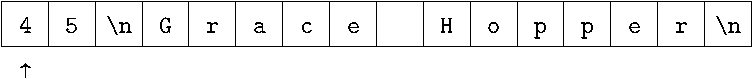
\includegraphics{figs/hopper1.pdf}
\caption{A stream of characters as seen by a \java{Scanner}.}
\label{fig.hopper1}
\end{center}
\end{figure}

%TODO define call/invoke or use other term?

The arrow indicates the next character to be read by \java{Scanner}.
When you call \java{nextInt}, it reads characters until it gets to a non-digit.
Figure~\ref{fig.hopper2} shows the state of the stream after \java{nextInt} is called.

\begin{figure}[!ht]
\begin{center}
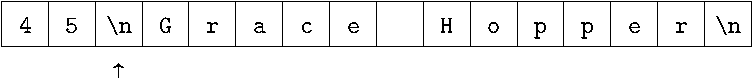
\includegraphics{figs/hopper2.pdf}
\caption{A stream of characters after \java{nextInt} is called.}
\label{fig.hopper2}
\end{center}
\end{figure}

At this point, \java{nextInt} returns \java{45}.
The program then displays the prompt \java{"What is your name? "} and calls \java{nextLine}, which reads characters until it gets to a newline.
But since the next character is already a newline, \java{nextLine} returns the empty string \java{""}.

To solve this problem, you need an extra \java{nextLine} after \java{nextInt}.

\begin{code}
System.out.print("What is your age? ");
age = in.nextInt();
in.nextLine();  // read the newline
System.out.print("What is your name? ");
name = in.nextLine();
System.out.printf("Hello %s, age %d\n", name, age);
\end{code}

This technique is common when reading \java{int} or \java{double} values that appear on their own line.
First you read the number, and then you read the rest of the line, which is just a newline character.


% DW suggests we also cover PrintWriter to write files --
% add an appendix on File I/O since it involves try/catch?

\section{Vocabulary}

\begin{description}

\term{package}
A directory of classes that are related to each other.
%Java classes are organized into packages.

\term{address}
The location of a value in computer memory, often represented as a hexadecimal integer.

\term{library}
A collection of packages and classes that are available for use in other programs.
%Libraries are often distributed in {\tt .jar} (Java Archive) files.

%\term{abstraction}
%The process of reducing information and/or detail to focus on high-level concepts.

%\term{operating system}
%Software that is always running behind the scenes on your computer.
%It controls the execution of application programs and manages hardware resources.

%\term{byte}
%A single unit of data on a computer; enough to represent one character.

%\term{utility class}
%A class that provides commonly needed functionality.

\term{import statement}
A statement that allows programs to use classes defined in other packages.

\term{token}
The smallest unit of source code, such as an individual word, literal value, or symbol.

%\term{syntax}
%The structure of a program; the arrangement of the words and symbols it contains.

%\term{semantics}
%The meaning of a program; the low-level instructions it should perform.

\term{literal}
A value that appears in source code.
For example, \java{"Hello"} is a string literal, and \java{74} is an integer literal.

\term{prompt}
A brief message displayed in a print statement that asks the user for input.

\term{magic number}
A number that appears without explanation as part of an expression.
It should generally be replaced with a constant.

\term{constant}
A variable, declared as \java{final}, whose value cannot be changed.

\term{format string}
The string in \java{System.out.printf} that specifies the format of the output.

\term{format specifier}
A special code that begins with a percent sign and specifies the data type and format of the corresponding value.

\term{type cast}
An operation that explicitly converts one data type into another.
In Java it appears as a type name in parentheses, like \java{(int)}.

%\term{truncate}
%To make shorter by cutting something off.
%Casting a floating-point value to an integer simply removes the fractional part.

\term{modulo}
An operation that yields the remainder when one integer is divided by another.
In Java, it is denoted with a percent sign: \java{5 \% 2} is \java{1}.

\term{modulus}
The value of \java{b} in the expression \java{a \% b}.
It often represents unit conversions, such as 24 hours in a day, 60 minutes in an hour, etc.

\end{description}


\section{Exercises}

The code for this chapter is in the {\tt ch03} directory of {\tt ThinkJavaCode2}.
See page~\pageref{code} for instructions on how to download the repository.
Before you start the exercises, we recommend that you compile and run the examples.

If you have not already read Appendix~\ref{commandline}, now might be a good time.
It describes the command-line interface, which is a powerful and efficient way to interact with your computer.


\begin{exercise}  %%V6 Ex3.1

When you use \java{printf}, the Java compiler does not check your format string.
See what happens if you try to display a value with type \java{int} using \java{\%f}.
And what happens if you display a \java{double} using \java{\%d}?
What if you use two format specifiers, but then only provide one value?

\end{exercise}

%If you try to print an integer with \java{\%f} or a floating-point number using \java{\%d}, you get an \java{IllegalFormatConversionException}.


\begin{exercise}  %%V6 Ex3.2

Write a program that converts a temperature from Celsius to Fahrenheit.
It should (1) prompt the user for input, (2) read a \java{double} value from the keyboard, (3) calculate the result, and (4) format the output to one decimal place.
For example, it should display {\tt "24.0 C = 75.2 F"}.

Here is the formula.
Be careful not to use integer division!
%
\[ F = C \times \frac{9}{5} + 32 \]

\end{exercise}


\begin{exercise}  %%V6 Ex3.3

Write a program that converts a total number of seconds to hours, minutes, and seconds.
It should (1) prompt the user for input, (2) read an integer from the keyboard, (3) calculate the result, and (4) use \java{printf} to display the output.
For example, {\tt "5000 seconds = 1 hours, 23 minutes, and 20 seconds"}.

{\it Hint:} Use the remainder operator.

\end{exercise}


\begin{exercise}  %%V6 Ex3.4
\label{guess}

The goal of this exercise is to program a ``Guess My Number'' game.
When it's finished, it will work like this:

\begin{stdout}
I'm thinking of a number between 1 and 100
(including both). Can you guess what it is?
Type a number: 45
Your guess is: 45
The number I was thinking of is: 14
You were off by: 31
\end{stdout}

To choose a random number, you can use the \java{Random} class in \java{java.util}.
Here's how it works:

\index{GuessStarter.java}

\begin{trinket}{GuessStarter.java}
import java.util.Random;

public class GuessStarter {

    public static void main(String[] args) {
        // pick a random number
        Random random = new Random();
        int number = random.nextInt(100) + 1;
        System.out.println(number);
    }
}
\end{trinket}

\index{new}
\index{operator!new}

Like the \java{Scanner} class we saw in this chapter, \java{Random} has to be imported before we can use it.
And as we saw with \java{Scanner}, we have to use the \java{new} operator to create a \java{Random} (number generator).

Then we can use the method \java{nextInt} to generate a random number.
In this example, the result of \java{nextInt(100)} will be between 0 and 99, including both.
Adding 1 yields a number between 1 and 100, including both.

\begin{enumerate}

\item The definition of \java{GuessStarter} is in a file called {\tt GuessStarter.java}, in the directory called {\tt ch03}, in the repository for this book.
%Instructions for downloading this code are on page~\pageref{code}.

\item Compile and run this program.

\item Modify the program to prompt the user, then use a \java{Scanner} to read a line of user input.
Compile and test the program.

\item Read the user input as an integer and display the result.
Again, compile and test.

\item Compute and display the difference between the user's guess and the number that was generated.

\end{enumerate}

\end{exercise}


\chapter{Void methods}
\label{voidmeth}

So far we've only written short programs that have a single class and a single method (\java{main}).
In this chapter, we'll show you how to organize longer programs into multiple methods and classes.
We'll also present the \java{Math} class, which provides methods for common mathematical operations.


%We will also take a look at separate compilation.
%At a conceptual level, a {\bf method} represents a mathematical {\em function} or a general {\em procedure}.
%Some methods perform a computation and return a result.
%For example, \java{Math.sqrt(25)} returns the value \java{5.0}.
%Other methods (including \java{main}) carry out a sequence of actions without returning a result.
%Java uses the keyword \java{void} to declare such methods.
%Regardless whether they return a value or not, methods enable you to break down a complex program into smaller blocks of code.


\section{Math methods}

\index{expression}
\index{argument}

In mathematics, you have probably seen functions like $\sin$ and $\log$, and you have learned to evaluate expressions like $\sin(\pi/2)$ and $\log(1/x)$.
First, you evaluate the expression in parentheses, which is called the {\bf argument} of the function.
Then you can evaluate the function itself, maybe by punching it into a calculator.

This process can be applied repeatedly to evaluate more complex expressions like $\log(1/\sin(\pi/2))$.
First we evaluate the argument of the innermost function, then evaluate the function itself, and so on.

\index{Math class}
\index{class!Math}
\index{invoke}

The Java library includes a \java{Math} class that provides common mathematical operations.
\java{Math} is in the \java{java.lang} package, so you don't have to import it.
You can use, or {\bf invoke}, \java{Math} methods like this:

\begin{code}
double root = Math.sqrt(17.0);
double angle = 1.5;
double height = Math.sin(angle);
\end{code}

The first line sets \java{root} to the square root of 17.
The third line finds the sine of 1.5 (the value of \java{angle}).

\index{degrees}
\index{radians}
\index{pi}

Arguments of the trigonometric functions -- \java{sin}, \java{cos}, and \java{tan} -- should be in {\em radians}.
To convert from degrees to radians, you can divide by 180 and multiply by $\pi$.
Conveniently, the \java{Math} class provides a constant double named \java{PI} that contains an approximation of $\pi$:

\begin{code}
double degrees = 90;
double angle = degrees / 180.0 * Math.PI;
\end{code}

Notice that \java{PI} is in capital letters.
Java does not recognize \java{Pi}, \java{pi}, or \java{pie}.
Also, \java{PI} is the name of a variable, not a method, so it doesn't have parentheses.
The same is true for the constant \java{Math.E}, which approximates Euler's number.

Converting to and from radians is a common operation, so the \java{Math} class provides methods that do it for you.

\begin{code}
double radians = Math.toRadians(180.0);
double degrees = Math.toDegrees(Math.PI);
\end{code}

\index{long}
\index{type!long}

Another useful method is \java{round}, which rounds a floating-point value to the nearest integer and returns a \java{long}.
A \java{long} is like an \java{int}, but bigger.
More specifically, an \java{int} uses 32 bits; the largest value it can hold is $2^{31}-1$, which is about 2 billion.
A \java{long} uses 64 bits, so the largest value is $2^{63}-1$, which is about 9 quintillion.

\begin{code}
long x = Math.round(Math.PI * 20.0);
\end{code}

The result is 63 (rounded up from 62.8319).

Take a minute to read the documentation for these and other methods in the \java{Math} class.
The easiest way to find documentation for Java classes is to do a web search for ``Java'' and the name of the class.


\section{Composition revisited}

\index{composition}
\index{expression}

Just as with mathematical functions, Java methods can be {\em composed}.
That means you can use one expression as part of another.
For example, you can use any expression as an argument to a method:

\begin{code}
double x = Math.cos(angle + Math.PI / 2.0);
\end{code}

This statement divides \java{Math.PI} by two, adds the result to \java{angle}, and computes the cosine of the sum.
You can also take the result of one method and pass it as an argument to another:

\begin{code}
double x = Math.exp(Math.log(10.0));
\end{code}

In Java, the \java{log} method always uses base $e$.
So this statement finds the log base $e$ of 10, and then raises $e$ to that power.
The result gets assigned to \java{x}.

Some math methods take more than one argument.
For example, \java{Math.pow} takes two arguments and raises the first to the power of the second.
This line of code assigns the value \java{1024.0} to the variable \java{x}:

\begin{code}
double x = Math.pow(2.0, 10.0);
\end{code}

When using \java{Math} methods, it is a common error to forget the \java{Math}.
For example, if you try to invoke \java{pow(2.0, 10.0)}, you get an error message like:

\begin{stdout}
File: Test.java  [line: 5]
Error: cannot find symbol
  symbol:   method pow(double,double)
  location: class Test
\end{stdout}

The message ``cannot find symbol'' is confusing, but the last line provides a useful hint.
The compiler is looking for \java{pow} in the same class where it is used, which is \java{Test}.
If you don't specify a class name, the compiler looks in the current class.


\section{Adding new methods}
\label{adding_methods}

\index{method!definition}

You have probably guessed by now that you can define more than one method in a class.
Here's an example:

\begin{trinket}[310]{NewLine.java}
public class NewLine {

    public static void newLine() {
        System.out.println();
    }

    public static void main(String[] args) {
        System.out.println("First line.");
        newLine();
        System.out.println("Second line.");
    }
}
\end{trinket}

\index{main}
\index{case-sensitive}

The name of the class is \java{NewLine}.
By convention, class names begin with a capital letter.
\java{NewLine} contains two methods, \java{newLine} and \java{main}.
Remember that Java is case-sensitive, so \java{NewLine} and \java{newLine} are not the same.

\index{camel case}

Method names should begin with a lowercase letter and use ``camel case'', which is a cute name for \java{jammingWordsTogetherLikeThis}.
You can use any name you want for methods, except \java{main} or any of the Java keywords.

\index{public}
\index{void}
\index{type!void}

\java{newLine} and \java{main} are \java{public}, which means they can be invoked from other classes.
They are both \java{static}, but we can't explain what that means yet.
And they are both \java{void}, which means that they don't yield a result (unlike the \java{Math} methods, for example).

\index{parameter}

The parentheses after the method name contain a list of variables, called {\bf parameters}, where the method stores its arguments.
\java{main} has a single parameter, called \java{args}, which has type \java{String[]}.
That means that whoever invokes \java{main} must provide an array of strings (we'll get to arrays in a later chapter).

Since \java{newLine} has no parameters, it requires no arguments, as shown when it is invoked in \java{main}.
And because \java{newLine} is in the same class as \java{main}, we don't have to specify the class name.

The output of this program is:

\begin{stdout}
First line.

Second line.
\end{stdout}

Notice the extra space between the lines.
If we wanted more space between them, we could invoke the same method repeatedly:

\begin{code}
public static void main(String[] args) {
    System.out.println("First line.");
    newLine();
    newLine();
    newLine();
    System.out.println("Second line.");
}
\end{code}

Or we could write a new method that displays three blank lines:

\begin{code}
public static void threeLine() {
    newLine();
    newLine();
    newLine();
}

public static void main(String[] args) {
    System.out.println("First line.");
    threeLine();
    System.out.println("Second line.");
}
\end{code}

You can invoke the same method more than once, and you can have one method invoke another.
In this example, \java{main} invokes \java{threeLine}, and \java{threeLine} invokes \java{newLine}.

Beginners often wonder why it is worth the trouble to create new methods.
There are many reasons, but this example demonstrates a few of them:

\begin{itemize}

\item Creating a new method gives you an opportunity to give a name to a group of statements, which makes code easier to read and understand.
%Methods simplify a program by hiding complex computations behind a single statement, and by using English words in place of arcane code.
%Which is clearer, \java{newLine} or \java{System.out.println()}?

\item Introducing new methods can make a program smaller by eliminating repetitive code.
For example, to display nine consecutive new lines, you could invoke \java{threeLine} three times.

\item A common problem solving technique is to break tasks down into sub-problems.
Methods allow you to focus on each sub-problem in isolation, and then compose them into a complete solution.

\end{itemize}

%Perhaps most importantly, organizing your code into multiple methods allows you to test individual parts of your program separately.
%It's easier to get a complex program working if you know that each sub-part works correctly.

%In Section~\ref{methods} we will come back to this question and list some additional benefits of dividing programs into methods.


\section{Flow of execution}

\index{class}
\index{method}

Pulling together the code from the previous section, the complete program looks like this:

\begin{trinket}{NewLine.java}
public class NewLine {

    public static void newLine() {
        System.out.println();
    }

    public static void threeLine() {
        newLine();
        newLine();
        newLine();
    }

    public static void main(String[] args) {
        System.out.println("First line.");
        threeLine();
        System.out.println("Second line.");
    }
}
\end{trinket}

\index{flow of execution}

When you look at a class definition that contains several methods, it is tempting to read it from top to bottom.
But that is likely to be confusing, because that is not the {\bf flow of execution} of the program.

Execution always begins at the first statement of \java{main}, regardless of where it is in the source file.
Statements are executed one at a time, in order, until you reach a method invocation, which you can think of as a detour.
Instead of going to the next statement, you jump to the first line of the invoked method, execute all the statements there, and then come back and pick up exactly where you left off.

That sounds simple enough, but remember that one method can invoke another one.
In the middle of \java{main}, we go off to execute the statements in \java{threeLine}.
While we are executing \java{threeLine}, we go off to execute \java{newLine}.
Then \java{newLine} invokes \java{println}, which causes yet another detour.

Fortunately, Java is good at keeping track of which methods are running.
So when \java{println} completes, it picks up where it left off in \java{newLine}; when \java{newLine} completes, it goes back to \java{threeLine}, and when \java{threeLine} completes, it gets back to \java{main}.

In summary, when you read a program, don't read from top to bottom.
Instead, follow the flow of execution.

%Technically, the program does not terminate at the end of \java{main}.
%Instead, execution picks up where it left off in the program that invoked \java{main}, which is the Java interpreter.
%The interpreter takes care of things like deleting windows and general cleanup, and {\em then} the program terminates.


\section{Parameters and arguments}

\index{parameter}
\index{argument}

Some of the methods we have used require arguments, which are the values you provide when you invoke the method.
For example, to find the sine of a number, you have to provide the number, so \java{sin} takes a \java{double} as an argument.
To display a message, you have to provide the message, so \java{println} takes a \java{String}.

When you use a method, you provide the arguments.
When you write a method, you name the parameters.
The parameter list indicates what arguments are required.
The following class shows an example:

\begin{trinket}[295]{PrintTwice.java}
public class PrintTwice {

    public static void printTwice(String s) {
        System.out.println(s);
        System.out.println(s);
    }

    public static void main(String[] args) {
        printTwice("Don't make me say this twice!");
    }
}
\end{trinket}

\java{printTwice} has a parameter named \java{s} with type \java{String}.
When we invoke \java{printTwice}, we have to provide an argument with type \java{String}.

Before the method executes, the argument gets assigned to the parameter.
In this example, the argument \java{"Don't make me say this twice!"} gets assigned to the parameter \java{s}.

\index{parameter passing}

This process is called {\bf parameter passing} because the value gets passed from outside the method to the inside.
An argument can be any kind of expression, so if you have a \java{String} variable, you can use it as an argument:

\begin{code}
String argument = "Never say never.";
printTwice(argument);
\end{code}

The value you provide as an argument must have the same type as the parameter.
For example, if you try:

\begin{code}
printTwice(17);  // syntax error
\end{code}

You will get an error message like this:

\begin{stdout}
File: Test.java  [line: 10]
Error: method printTwice in class Test cannot be applied
       to given types;
  required: java.lang.String
  found: int
  reason: actual argument int cannot be converted to
          java.lang.String by method invocation conversion
\end{stdout}

Sometimes Java can convert an argument from one type to another automatically.
For example, \java{Math.sqrt} requires a \java{double}, but if you invoke \java{Math.sqrt(25)}, the integer value \java{25} is automatically converted to the floating-point value \java{25.0}.
But in the case of \java{printTwice}, Java can't (or won't) convert the integer \java{17} to a \java{String}.

Parameters and other variables only exist inside their own methods.
Inside \java{main}, there is no such thing as \java{s}.
If you try to use it there, you'll get a compiler error.
Similarly, inside \java{printTwice} there is no such thing as \java{argument}.
That variable belongs to \java{main}.

\index{local variable}
\index{variable!local}

Because variables only exist inside the methods where they are defined, they are often called {\bf local variables}.


\section{Multiple parameters}
\label{time}

\index{parameter!multiple}
\index{method!parameters}

Here is an example of a method that takes two parameters:

\begin{code}
public static void printTime(int hour, int minute) {
    System.out.print(hour);
    System.out.print(":");
    System.out.println(minute);
}
\end{code}

In the parameter list, it may be tempting to write:

\begin{code}
public static void printTime(int hour, minute) {
    ...
\end{code}

But that format (without the second \java{int}) is only legal for variable declarations.
In parameter lists, you need to specify the type of each variable separately.

To invoke this method, we have to provide two integers as arguments:

\begin{code}
int hour = 11;
int minute = 59;
printTime(hour, minute);
\end{code}

A common error is to declare the types of the arguments, like this:

\begin{code}
int hour = 11;
int minute = 59;
printTime(int hour, int minute);  // syntax error
\end{code}

That's a syntax error; the compiler sees \java{int hour} and \java{int minute} as variable declarations, not expressions.
You wouldn't declare the types of the arguments if they were simply integers:

\begin{code}
printTime(int 11, int 59);  // syntax error
\end{code}


\section{Stack diagrams}
\label{stack}

Pulling together the code fragments from the previous section, here is a complete class definition:

\begin{trinket}[340]{PrintTime.java}
public class PrintTime {

    public static void printTime(int hour, int minute) {
        System.out.print(hour);
        System.out.print(":");
        System.out.println(minute);
    }

    public static void main(String[] args) {
        int hour = 11;
        int minute = 59;
        printTime(hour, minute);
    }
}
\end{trinket}

\java{printTime} has two parameters, named \java{hour} and \java{minute}.
And \java{main} has two variables, also named \java{hour} and \java{minute}.
Although they have the same names, these variables are not the same.
\java{hour} in \java{printTime} and \java{hour} in \java{main} refer to different storage locations, and they can have different values.

For example, you could invoke \java{printTime} like this:

\begin{code}
int hour = 11;
int minute = 59;
printTime(hour + 1, 0);
\end{code}

Before the method is invoked, Java evaluates the arguments; in this example, the results are \java{12} and \java{0}.
Then it assigns those values to the parameters.
Inside \java{printTime}, the value of \java{hour} is \java{12}, not \java{11}, and the value of \java{minute} is \java{0}, not \java{59}.
Furthermore, if \java{printTime} modifies one of its parameters, that change has no effect on the variables in \java{main}.

\index{stack diagram}
\index{diagram!stack}
\index{frame}

One way to keep track of everything is to draw a {\bf stack diagram}, which is a state diagram (see Section~\ref{state}) that shows method invocations.
For each method there is a box called a {\bf frame} that contains the method's parameters and variables.
The name of the method appears outside the frame; the variables and parameters appear inside.

\begin{figure}[!ht]
\begin{center}
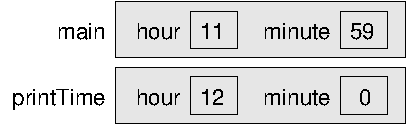
\includegraphics[scale=0.9]{figs/stack.pdf}
\caption{Stack diagram for \java{PrintTime}.}
\label{fig.stack}
\end{center}
\end{figure}

As with state diagrams, stack diagrams show variables and methods at a particular point in time.
Figure~\ref{fig.stack} is a stack diagram at the beginning of the \java{printTime} method.

%\index{scope}

%Stack diagrams help you to visualize the {\bf scope} of a variable, which is the area of a program where a variable exists.


\section{Reading documentation}
\label{sec:apidocs}

\index{documentation}

One of the nice things about Java is that it comes with an extensive library of classes and methods.
But before you use them, you might have to read the documentation.
And sometimes that's not easy.

As an example, let's look at the documentation for \java{Scanner}, which we used in Section~\ref{scanner}.
You can find it by doing a web search for ``Java Scanner''.
Figure~\ref{fig.scanner} shows a screenshot of the page.

\begin{figure}[!ht]
\begin{center}
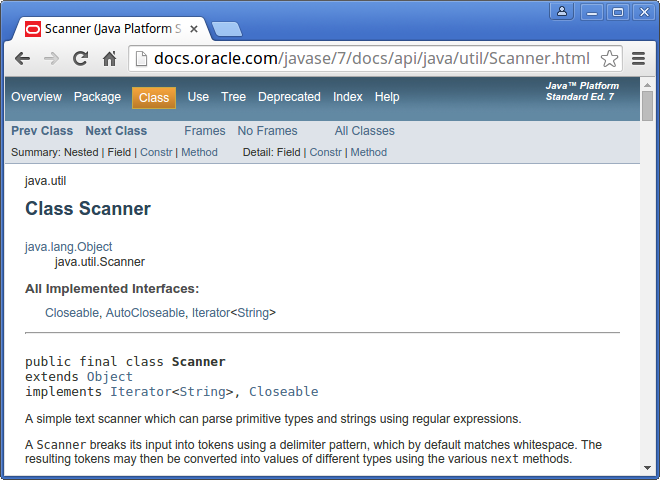
\includegraphics[width=0.9\textwidth]{figs/scanner.png}
\caption{Screenshot of the documentation for \java{Scanner}.}
\label{fig.scanner}
\end{center}
\end{figure}

Documentation for other classes uses a similar format.
The first line is the package that contains the class, such as \java{java.util}.
The second line is the name of the class.
The ``Implemented Interfaces'' section lists some of the things a \java{Scanner} can do; we won't say more about that for now.

%The next two lines indicate that every \java{Scanner} is also an \java{Object}; that will make more sense after Section~\ref{inheritance}.

The next section of the documentation is a narrative that explains the purpose of the class and includes examples of how to use it.
This text can be difficult to read because it uses terms we have not learned yet.
But the examples are often very useful.
A good way to get started with a new class is to paste the examples into a test file and see if you can compile and run them.

One of the examples shows how you can use a \java{Scanner} to read input from a \java{String} instead of \java{System.in}:

%NOTE: only use of Scanner w/o System.in; mention this again in String chapter?
\begin{code}
String input = "1 fish 2 fish red fish blue fish";
Scanner s = new Scanner(input);
\end{code}

After the narrative, code examples, and some other details, you will find the following tables:

\begin{description}

\item[Constructor summary:]
Ways of creating, or ``constructing'', a \java{Scanner}.

\item[Method summary:]
The list of methods that \java{Scanner} provides.

\item[Constructor detail:]
More information about how to create a \java{Scanner}.

\item[Method detail:]
More information about each method.

\end{description}

As an example, here is the summary information for \java{nextInt}:

\begin{stdout}
public int nextInt()
Scans the next token of the input as an int.
\end{stdout}

\index{signature}

The first line is the method's {\bf signature}, which specifies the name of the method, its parameters (none), and what type it returns (\java{int}).
The next line is a short description of what it does.

The ``Method detail'' explains more:

\begin{stdout}
public int nextInt()
Scans the next token of the input as an int.

An invocation of this method of the form nextInt() behaves in
exactly the same way as the invocation nextInt(radix), where
radix is the default radix of this scanner.

Returns:
the int scanned from the input

Throws:
InputMismatchException - if the next token does not match
    the Integer regular expression, or is out of range
NoSuchElementException - if input is exhausted
IllegalStateException - if this scanner is closed
\end{stdout}

The ``Returns'' section describes the result when the method succeeds.
In contrast, the ``Throws'' section describes possible errors and their resulting exceptions.
Exceptions are said to be ``thrown'', like a referee throwing a flag, or like a toddler throwing a fit.

It might take you some time to get comfortable reading documentation and learning which parts to ignore.
But it's worth the effort.
Knowing what's available in the library helps you avoid reinventing the wheel.
And a little bit of documentation can save you a lot of debugging.


\section{Writing documentation}
\label{sec:javadoc}

As you benefit from reading good documentation, you should ``pay it forward'' by writing good documentation.
A nice feature of the Java language is the ability to embed documentation in your source code.
That way, you can write it as you go, and as things change, it is easier to keep the documentation consistent with the code.

\index{HTML}
\index{Javadoc}

If you include documentation in your source code, you can extract it automatically, and generate well-formatted HTML, using a tool called {\bf Javadoc}.
This tool is included in standard Java development environments, and it is widely used.
In fact, the online documentation of the Java libraries is generated by Javadoc.

\index{comment!documentation}
\index{documentation!Javadoc comments}

Javadoc scans your source files looking for specially-formatted {\bf documentation comments}, also known as ``Javadoc comments''.
They begin with \java{/**} (two stars) and end with \java{*/} (one star).
Anything in between is considered part of the documentation.

Here's a class definition with two Javadoc comments, one for the class and one for the \java{main} method:

\begin{code}
/**
 * Example program that demonstrates print vs println.
 */
public class Goodbye {

    /**
     * Prints a greeting.
     */
    public static void main(String[] args) {
        System.out.print("Goodbye, ");  // note the space
        System.out.println("cruel world");
    }
}
\end{code}

The class comment explains the purpose of the class.
The method comment explains what the method does.

Notice that this example also includes an inline comment, beginning with \java{//}.
In general, inline comments are short phrases that help explain complex parts of a program.
They are intended for other programmers reading and maintaining the source code.

In contrast, Javadoc comments are longer, usually complete sentences.
They explain what each method does, but they omit details about how the method works.
And they are intended for people who will use the methods without looking at the source code.

Appropriate comments and documentation are essential for making source code readable.
And remember that the person most likely to read your code in the future, and appreciate good documentation, is you.


\section{Vocabulary}

\begin{description}

% Note: expanded definition from Chapter 1
%\term{method}
%A named sequence of statements that performs a procedure or function.
%Methods may or may not take parameters, and may or may not return a value.

\term{argument}
A value that you provide when you invoke a method.
This value must have the same type as the corresponding parameter.

\term{invoke}
To cause a method to execute.
Also known as ``calling'' a method.

\term{parameter}
A piece of information that a method requires before it can run.
Parameters are variables: they contain values and have types.

% Note: expanded definition from Chapter 2
%\term{composition}
%The ability to combine simple expressions and statements into compound %expressions and statements, making it possible to use intermediate %computations as arguments.

\term{flow of execution}
The order in which Java executes methods and statements.
It may not necessarily be from top to bottom, left to right.

\term{parameter passing}
The process of assigning an argument value to a parameter variable.

\term{local variable}
A variable declared inside a method.
Local variables cannot be accessed from outside their method.

\term{stack diagram}
A graphical representation of the variables belonging to each method.
The method calls are ``stacked'' from top to bottom, in the flow of execution.

\term{frame}
In a stack diagram, a representation of the variables and parameters for a method, along with their current values.

%\term{scope}
%The area of a program where a variable exists.

\term{signature}
The first line of a method that defines its name, return type, and parameters.

\term{Javadoc}
A tool that reads Java source code and generates documentation in HTML format.

\term{documentation}
Comments that describe the technical operation of a class or method.

\end{description}


\section{Exercises}

The code for this chapter is in the {\tt ch04} directory of {\tt ThinkJavaCode}.
See page~\pageref{code} for instructions on how to download the repository.
Before you start the exercises, we recommend that you compile and run the examples.

If you have not already read Appendix~\ref{cltesting}, now might be a good time.
It describes an efficient way to test programs that take input from the user and display specific output.


\begin{exercise}

The point of this exercise is to practice reading code and to make sure that you understand the flow of execution through a program with multiple methods.

\begin{enumerate}

\item What is the output of the following program?
Be precise about where there are spaces and where there are newlines.

{\it Hint:} Start by describing in words what \java{ping} and \java{baffle} do when they are invoked.

\item Draw a stack diagram that shows the state of the program the first time \java{ping} is invoked.

\item What happens if you invoke \java{baffle();} at the end of the \java{ping} method? (We will see why in the next chapter.)

\end{enumerate}

\begin{code}
public static void zoop() {
    baffle();
    System.out.print("You wugga ");
    baffle();
}

public static void main(String[] args) {
    System.out.print("No, I ");
    zoop();
    System.out.print("I ");
    baffle();
}

public static void baffle() {
    System.out.print("wug");
    ping();
}

public static void ping() {
    System.out.println(".");
}
\end{code}

\end{exercise}


%\begin{exercise}

%What is the difference between a variable and a method?
%In terms of their syntax, how does the Java compiler tell the difference between the two?

%%A variable is a {\em location of data}, whereas a method is a {\em location of code}.
%%In Java, methods always have parentheses, even if they have no arguments like \java{System.out.println()}.

%\end{exercise}


%ABD: We don't need this anymore since we used this as an example
%\begin{exercise}
%Draw a stack diagram that shows the state of the program in Section~\ref{time} when \java{main} invokes \java{printTime} with the arguments \java{11} and \java{59}.
%\end{exercise}


\begin{exercise}

The point of this exercise is to make sure you understand how to write and invoke methods that take parameters.

\begin{enumerate}
\item Write the first line of a method named \java{zool} that takes three parameters: an \java{int} and two \java{String}s.

\item Write a line of code that calls \java{zool}, passing as arguments the value \java{11}, the name of your first pet, and the name of the street you grew up on.
\end{enumerate}

\end{exercise}


\begin{exercise}

The purpose of this exercise is to take code from a previous exercise and encapsulate it in a method that takes parameters.
You should start with a working solution to Exercise~\ref{ex:date}.

\begin{enumerate}

\item Write a method called \java{printAmerican} that takes the day, date, month and year as parameters and that displays them in American format.

\item Test your method by invoking it from \java{main} and passing appropriate arguments.
The output should look something like this (except that the date might be different):

\begin{stdout}
Saturday, July 22, 2015
\end{stdout}

\item Once you have debugged \java{printAmerican}, write another method called \java{printEuropean} that displays the date in European format.

\end{enumerate}

\end{exercise}


\chapter{Void methods}
\label{voidmeth}

So far we've only written short programs that have a single class and a single method (\java{main}).
In this chapter, we'll show you how to organize longer programs into multiple methods and classes.
We'll also present the \java{Math} class, which provides methods for common mathematical operations.


%We will also take a look at separate compilation.
%At a conceptual level, a {\bf method} represents a mathematical {\em function} or a general {\em procedure}.
%Some methods perform a computation and return a result.
%For example, \java{Math.sqrt(25)} returns the value \java{5.0}.
%Other methods (including \java{main}) carry out a sequence of actions without returning a result.
%Java uses the keyword \java{void} to declare such methods.
%Regardless whether they return a value or not, methods enable you to break down a complex program into smaller blocks of code.


\section{Math methods}

\index{expression}
\index{argument}

In mathematics, you have probably seen functions like $\sin$ and $\log$, and you have learned to evaluate expressions like $\sin(\pi/2)$ and $\log(1/x)$.
First, you evaluate the expression in parentheses, which is called the {\bf argument} of the function.
Then you can evaluate the function itself, maybe by punching it into a calculator.

This process can be applied repeatedly to evaluate more complex expressions like $\log(1/\sin(\pi/2))$.
First we evaluate the argument of the innermost function, then evaluate the function itself, and so on.

\index{Math class}
\index{class!Math}
\index{invoke}

The Java library includes a \java{Math} class that provides common mathematical operations.
\java{Math} is in the \java{java.lang} package, so you don't have to import it.
You can use, or {\bf invoke}, \java{Math} methods like this:

\begin{code}
double root = Math.sqrt(17.0);
double angle = 1.5;
double height = Math.sin(angle);
\end{code}

The first line sets \java{root} to the square root of 17.
The third line finds the sine of 1.5 (the value of \java{angle}).

\index{degrees}
\index{radians}
\index{pi}

Arguments of the trigonometric functions -- \java{sin}, \java{cos}, and \java{tan} -- should be in {\em radians}.
To convert from degrees to radians, you can divide by 180 and multiply by $\pi$.
Conveniently, the \java{Math} class provides a constant double named \java{PI} that contains an approximation of $\pi$:

\begin{code}
double degrees = 90;
double angle = degrees / 180.0 * Math.PI;
\end{code}

Notice that \java{PI} is in capital letters.
Java does not recognize \java{Pi}, \java{pi}, or \java{pie}.
Also, \java{PI} is the name of a variable, not a method, so it doesn't have parentheses.
The same is true for the constant \java{Math.E}, which approximates Euler's number.

Converting to and from radians is a common operation, so the \java{Math} class provides methods that do it for you.

\begin{code}
double radians = Math.toRadians(180.0);
double degrees = Math.toDegrees(Math.PI);
\end{code}

\index{long}
\index{type!long}

Another useful method is \java{round}, which rounds a floating-point value to the nearest integer and returns a \java{long}.
A \java{long} is like an \java{int}, but bigger.
More specifically, an \java{int} uses 32 bits; the largest value it can hold is $2^{31}-1$, which is about 2 billion.
A \java{long} uses 64 bits, so the largest value is $2^{63}-1$, which is about 9 quintillion.

\begin{code}
long x = Math.round(Math.PI * 20.0);
\end{code}

The result is 63 (rounded up from 62.8319).

Take a minute to read the documentation for these and other methods in the \java{Math} class.
The easiest way to find documentation for Java classes is to do a web search for ``Java'' and the name of the class.


\section{Composition revisited}

\index{composition}
\index{expression}

Just as with mathematical functions, Java methods can be {\em composed}.
That means you can use one expression as part of another.
For example, you can use any expression as an argument to a method:

\begin{code}
double x = Math.cos(angle + Math.PI / 2.0);
\end{code}

This statement divides \java{Math.PI} by two, adds the result to \java{angle}, and computes the cosine of the sum.
You can also take the result of one method and pass it as an argument to another:

\begin{code}
double x = Math.exp(Math.log(10.0));
\end{code}

In Java, the \java{log} method always uses base $e$.
So this statement finds the log base $e$ of 10, and then raises $e$ to that power.
The result gets assigned to \java{x}.

Some math methods take more than one argument.
For example, \java{Math.pow} takes two arguments and raises the first to the power of the second.
This line of code assigns the value \java{1024.0} to the variable \java{x}:

\begin{code}
double x = Math.pow(2.0, 10.0);
\end{code}

When using \java{Math} methods, it is a common error to forget the \java{Math}.
For example, if you try to invoke \java{pow(2.0, 10.0)}, you get an error message like:

\begin{stdout}
File: Test.java  [line: 5]
Error: cannot find symbol
  symbol:   method pow(double,double)
  location: class Test
\end{stdout}

The message ``cannot find symbol'' is confusing, but the last line provides a useful hint.
The compiler is looking for \java{pow} in the same class where it is used, which is \java{Test}.
If you don't specify a class name, the compiler looks in the current class.


\section{Adding new methods}
\label{adding_methods}

\index{method!definition}

You have probably guessed by now that you can define more than one method in a class.
Here's an example:

\begin{trinket}[310]{NewLine.java}
public class NewLine {

    public static void newLine() {
        System.out.println();
    }

    public static void main(String[] args) {
        System.out.println("First line.");
        newLine();
        System.out.println("Second line.");
    }
}
\end{trinket}

\index{main}
\index{case-sensitive}

The name of the class is \java{NewLine}.
By convention, class names begin with a capital letter.
\java{NewLine} contains two methods, \java{newLine} and \java{main}.
Remember that Java is case-sensitive, so \java{NewLine} and \java{newLine} are not the same.

\index{camel case}

Method names should begin with a lowercase letter and use ``camel case'', which is a cute name for \java{jammingWordsTogetherLikeThis}.
You can use any name you want for methods, except \java{main} or any of the Java keywords.

\index{public}
\index{void}
\index{type!void}

\java{newLine} and \java{main} are \java{public}, which means they can be invoked from other classes.
They are both \java{static}, but we can't explain what that means yet.
And they are both \java{void}, which means that they don't yield a result (unlike the \java{Math} methods, for example).

\index{parameter}

The parentheses after the method name contain a list of variables, called {\bf parameters}, where the method stores its arguments.
\java{main} has a single parameter, called \java{args}, which has type \java{String[]}.
That means that whoever invokes \java{main} must provide an array of strings (we'll get to arrays in a later chapter).

Since \java{newLine} has no parameters, it requires no arguments, as shown when it is invoked in \java{main}.
And because \java{newLine} is in the same class as \java{main}, we don't have to specify the class name.

The output of this program is:

\begin{stdout}
First line.

Second line.
\end{stdout}

Notice the extra space between the lines.
If we wanted more space between them, we could invoke the same method repeatedly:

\begin{code}
public static void main(String[] args) {
    System.out.println("First line.");
    newLine();
    newLine();
    newLine();
    System.out.println("Second line.");
}
\end{code}

Or we could write a new method that displays three blank lines:

\begin{code}
public static void threeLine() {
    newLine();
    newLine();
    newLine();
}

public static void main(String[] args) {
    System.out.println("First line.");
    threeLine();
    System.out.println("Second line.");
}
\end{code}

You can invoke the same method more than once, and you can have one method invoke another.
In this example, \java{main} invokes \java{threeLine}, and \java{threeLine} invokes \java{newLine}.

Beginners often wonder why it is worth the trouble to create new methods.
There are many reasons, but this example demonstrates a few of them:

\begin{itemize}

\item Creating a new method gives you an opportunity to give a name to a group of statements, which makes code easier to read and understand.
%Methods simplify a program by hiding complex computations behind a single statement, and by using English words in place of arcane code.
%Which is clearer, \java{newLine} or \java{System.out.println()}?

\item Introducing new methods can make a program smaller by eliminating repetitive code.
For example, to display nine consecutive new lines, you could invoke \java{threeLine} three times.

\item A common problem solving technique is to break tasks down into sub-problems.
Methods allow you to focus on each sub-problem in isolation, and then compose them into a complete solution.

\end{itemize}

%Perhaps most importantly, organizing your code into multiple methods allows you to test individual parts of your program separately.
%It's easier to get a complex program working if you know that each sub-part works correctly.

%In Section~\ref{methods} we will come back to this question and list some additional benefits of dividing programs into methods.


\section{Flow of execution}

\index{class}
\index{method}

Pulling together the code from the previous section, the complete program looks like this:

\begin{trinket}{NewLine.java}
public class NewLine {

    public static void newLine() {
        System.out.println();
    }

    public static void threeLine() {
        newLine();
        newLine();
        newLine();
    }

    public static void main(String[] args) {
        System.out.println("First line.");
        threeLine();
        System.out.println("Second line.");
    }
}
\end{trinket}

\index{flow of execution}

When you look at a class definition that contains several methods, it is tempting to read it from top to bottom.
But that is likely to be confusing, because that is not the {\bf flow of execution} of the program.

Execution always begins at the first statement of \java{main}, regardless of where it is in the source file.
Statements are executed one at a time, in order, until you reach a method invocation, which you can think of as a detour.
Instead of going to the next statement, you jump to the first line of the invoked method, execute all the statements there, and then come back and pick up exactly where you left off.

That sounds simple enough, but remember that one method can invoke another one.
In the middle of \java{main}, we go off to execute the statements in \java{threeLine}.
While we are executing \java{threeLine}, we go off to execute \java{newLine}.
Then \java{newLine} invokes \java{println}, which causes yet another detour.

Fortunately, Java is good at keeping track of which methods are running.
So when \java{println} completes, it picks up where it left off in \java{newLine}; when \java{newLine} completes, it goes back to \java{threeLine}, and when \java{threeLine} completes, it gets back to \java{main}.

In summary, when you read a program, don't read from top to bottom.
Instead, follow the flow of execution.

%Technically, the program does not terminate at the end of \java{main}.
%Instead, execution picks up where it left off in the program that invoked \java{main}, which is the Java interpreter.
%The interpreter takes care of things like deleting windows and general cleanup, and {\em then} the program terminates.


\section{Parameters and arguments}

\index{parameter}
\index{argument}

Some of the methods we have used require arguments, which are the values you provide when you invoke the method.
For example, to find the sine of a number, you have to provide the number, so \java{sin} takes a \java{double} as an argument.
To display a message, you have to provide the message, so \java{println} takes a \java{String}.

When you use a method, you provide the arguments.
When you write a method, you name the parameters.
The parameter list indicates what arguments are required.
The following class shows an example:

\begin{trinket}[295]{PrintTwice.java}
public class PrintTwice {

    public static void printTwice(String s) {
        System.out.println(s);
        System.out.println(s);
    }

    public static void main(String[] args) {
        printTwice("Don't make me say this twice!");
    }
}
\end{trinket}

\java{printTwice} has a parameter named \java{s} with type \java{String}.
When we invoke \java{printTwice}, we have to provide an argument with type \java{String}.

Before the method executes, the argument gets assigned to the parameter.
In this example, the argument \java{"Don't make me say this twice!"} gets assigned to the parameter \java{s}.

\index{parameter passing}

This process is called {\bf parameter passing} because the value gets passed from outside the method to the inside.
An argument can be any kind of expression, so if you have a \java{String} variable, you can use it as an argument:

\begin{code}
String argument = "Never say never.";
printTwice(argument);
\end{code}

The value you provide as an argument must have the same type as the parameter.
For example, if you try:

\begin{code}
printTwice(17);  // syntax error
\end{code}

You will get an error message like this:

\begin{stdout}
File: Test.java  [line: 10]
Error: method printTwice in class Test cannot be applied
       to given types;
  required: java.lang.String
  found: int
  reason: actual argument int cannot be converted to
          java.lang.String by method invocation conversion
\end{stdout}

Sometimes Java can convert an argument from one type to another automatically.
For example, \java{Math.sqrt} requires a \java{double}, but if you invoke \java{Math.sqrt(25)}, the integer value \java{25} is automatically converted to the floating-point value \java{25.0}.
But in the case of \java{printTwice}, Java can't (or won't) convert the integer \java{17} to a \java{String}.

Parameters and other variables only exist inside their own methods.
Inside \java{main}, there is no such thing as \java{s}.
If you try to use it there, you'll get a compiler error.
Similarly, inside \java{printTwice} there is no such thing as \java{argument}.
That variable belongs to \java{main}.

\index{local variable}
\index{variable!local}

Because variables only exist inside the methods where they are defined, they are often called {\bf local variables}.


\section{Multiple parameters}
\label{time}

\index{parameter!multiple}
\index{method!parameters}

Here is an example of a method that takes two parameters:

\begin{code}
public static void printTime(int hour, int minute) {
    System.out.print(hour);
    System.out.print(":");
    System.out.println(minute);
}
\end{code}

In the parameter list, it may be tempting to write:

\begin{code}
public static void printTime(int hour, minute) {
    ...
\end{code}

But that format (without the second \java{int}) is only legal for variable declarations.
In parameter lists, you need to specify the type of each variable separately.

To invoke this method, we have to provide two integers as arguments:

\begin{code}
int hour = 11;
int minute = 59;
printTime(hour, minute);
\end{code}

A common error is to declare the types of the arguments, like this:

\begin{code}
int hour = 11;
int minute = 59;
printTime(int hour, int minute);  // syntax error
\end{code}

That's a syntax error; the compiler sees \java{int hour} and \java{int minute} as variable declarations, not expressions.
You wouldn't declare the types of the arguments if they were simply integers:

\begin{code}
printTime(int 11, int 59);  // syntax error
\end{code}


\section{Stack diagrams}
\label{stack}

Pulling together the code fragments from the previous section, here is a complete class definition:

\begin{trinket}[340]{PrintTime.java}
public class PrintTime {

    public static void printTime(int hour, int minute) {
        System.out.print(hour);
        System.out.print(":");
        System.out.println(minute);
    }

    public static void main(String[] args) {
        int hour = 11;
        int minute = 59;
        printTime(hour, minute);
    }
}
\end{trinket}

\java{printTime} has two parameters, named \java{hour} and \java{minute}.
And \java{main} has two variables, also named \java{hour} and \java{minute}.
Although they have the same names, these variables are not the same.
\java{hour} in \java{printTime} and \java{hour} in \java{main} refer to different storage locations, and they can have different values.

For example, you could invoke \java{printTime} like this:

\begin{code}
int hour = 11;
int minute = 59;
printTime(hour + 1, 0);
\end{code}

Before the method is invoked, Java evaluates the arguments; in this example, the results are \java{12} and \java{0}.
Then it assigns those values to the parameters.
Inside \java{printTime}, the value of \java{hour} is \java{12}, not \java{11}, and the value of \java{minute} is \java{0}, not \java{59}.
Furthermore, if \java{printTime} modifies one of its parameters, that change has no effect on the variables in \java{main}.

\index{stack diagram}
\index{diagram!stack}
\index{frame}

One way to keep track of everything is to draw a {\bf stack diagram}, which is a state diagram (see Section~\ref{state}) that shows method invocations.
For each method there is a box called a {\bf frame} that contains the method's parameters and variables.
The name of the method appears outside the frame; the variables and parameters appear inside.

\begin{figure}[!ht]
\begin{center}
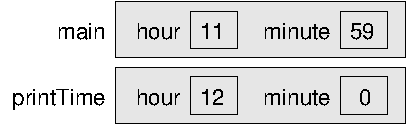
\includegraphics[scale=0.9]{figs/stack.pdf}
\caption{Stack diagram for \java{PrintTime}.}
\label{fig.stack}
\end{center}
\end{figure}

As with state diagrams, stack diagrams show variables and methods at a particular point in time.
Figure~\ref{fig.stack} is a stack diagram at the beginning of the \java{printTime} method.

%\index{scope}

%Stack diagrams help you to visualize the {\bf scope} of a variable, which is the area of a program where a variable exists.


\section{Reading documentation}
\label{sec:apidocs}

\index{documentation}

One of the nice things about Java is that it comes with an extensive library of classes and methods.
But before you use them, you might have to read the documentation.
And sometimes that's not easy.

As an example, let's look at the documentation for \java{Scanner}, which we used in Section~\ref{scanner}.
You can find it by doing a web search for ``Java Scanner''.
Figure~\ref{fig.scanner} shows a screenshot of the page.

\begin{figure}[!ht]
\begin{center}
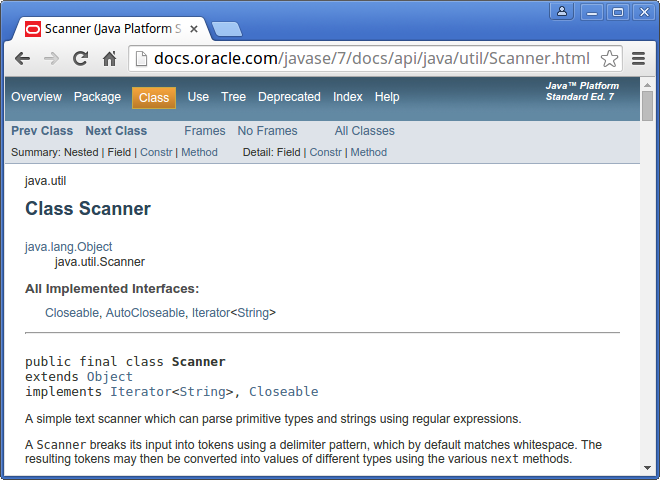
\includegraphics[width=0.9\textwidth]{figs/scanner.png}
\caption{Screenshot of the documentation for \java{Scanner}.}
\label{fig.scanner}
\end{center}
\end{figure}

Documentation for other classes uses a similar format.
The first line is the package that contains the class, such as \java{java.util}.
The second line is the name of the class.
The ``Implemented Interfaces'' section lists some of the things a \java{Scanner} can do; we won't say more about that for now.

%The next two lines indicate that every \java{Scanner} is also an \java{Object}; that will make more sense after Section~\ref{inheritance}.

The next section of the documentation is a narrative that explains the purpose of the class and includes examples of how to use it.
This text can be difficult to read because it uses terms we have not learned yet.
But the examples are often very useful.
A good way to get started with a new class is to paste the examples into a test file and see if you can compile and run them.

One of the examples shows how you can use a \java{Scanner} to read input from a \java{String} instead of \java{System.in}:

%NOTE: only use of Scanner w/o System.in; mention this again in String chapter?
\begin{code}
String input = "1 fish 2 fish red fish blue fish";
Scanner s = new Scanner(input);
\end{code}

After the narrative, code examples, and some other details, you will find the following tables:

\begin{description}

\item[Constructor summary:]
Ways of creating, or ``constructing'', a \java{Scanner}.

\item[Method summary:]
The list of methods that \java{Scanner} provides.

\item[Constructor detail:]
More information about how to create a \java{Scanner}.

\item[Method detail:]
More information about each method.

\end{description}

As an example, here is the summary information for \java{nextInt}:

\begin{stdout}
public int nextInt()
Scans the next token of the input as an int.
\end{stdout}

\index{signature}

The first line is the method's {\bf signature}, which specifies the name of the method, its parameters (none), and what type it returns (\java{int}).
The next line is a short description of what it does.

The ``Method detail'' explains more:

\begin{stdout}
public int nextInt()
Scans the next token of the input as an int.

An invocation of this method of the form nextInt() behaves in
exactly the same way as the invocation nextInt(radix), where
radix is the default radix of this scanner.

Returns:
the int scanned from the input

Throws:
InputMismatchException - if the next token does not match
    the Integer regular expression, or is out of range
NoSuchElementException - if input is exhausted
IllegalStateException - if this scanner is closed
\end{stdout}

The ``Returns'' section describes the result when the method succeeds.
In contrast, the ``Throws'' section describes possible errors and their resulting exceptions.
Exceptions are said to be ``thrown'', like a referee throwing a flag, or like a toddler throwing a fit.

It might take you some time to get comfortable reading documentation and learning which parts to ignore.
But it's worth the effort.
Knowing what's available in the library helps you avoid reinventing the wheel.
And a little bit of documentation can save you a lot of debugging.


\section{Writing documentation}
\label{sec:javadoc}

As you benefit from reading good documentation, you should ``pay it forward'' by writing good documentation.
A nice feature of the Java language is the ability to embed documentation in your source code.
That way, you can write it as you go, and as things change, it is easier to keep the documentation consistent with the code.

\index{HTML}
\index{Javadoc}

If you include documentation in your source code, you can extract it automatically, and generate well-formatted HTML, using a tool called {\bf Javadoc}.
This tool is included in standard Java development environments, and it is widely used.
In fact, the online documentation of the Java libraries is generated by Javadoc.

\index{comment!documentation}
\index{documentation!Javadoc comments}

Javadoc scans your source files looking for specially-formatted {\bf documentation comments}, also known as ``Javadoc comments''.
They begin with \java{/**} (two stars) and end with \java{*/} (one star).
Anything in between is considered part of the documentation.

Here's a class definition with two Javadoc comments, one for the class and one for the \java{main} method:

\begin{code}
/**
 * Example program that demonstrates print vs println.
 */
public class Goodbye {

    /**
     * Prints a greeting.
     */
    public static void main(String[] args) {
        System.out.print("Goodbye, ");  // note the space
        System.out.println("cruel world");
    }
}
\end{code}

The class comment explains the purpose of the class.
The method comment explains what the method does.

Notice that this example also includes an inline comment, beginning with \java{//}.
In general, inline comments are short phrases that help explain complex parts of a program.
They are intended for other programmers reading and maintaining the source code.

In contrast, Javadoc comments are longer, usually complete sentences.
They explain what each method does, but they omit details about how the method works.
And they are intended for people who will use the methods without looking at the source code.

Appropriate comments and documentation are essential for making source code readable.
And remember that the person most likely to read your code in the future, and appreciate good documentation, is you.


\section{Vocabulary}

\begin{description}

% Note: expanded definition from Chapter 1
%\term{method}
%A named sequence of statements that performs a procedure or function.
%Methods may or may not take parameters, and may or may not return a value.

\term{argument}
A value that you provide when you invoke a method.
This value must have the same type as the corresponding parameter.

\term{invoke}
To cause a method to execute.
Also known as ``calling'' a method.

\term{parameter}
A piece of information that a method requires before it can run.
Parameters are variables: they contain values and have types.

% Note: expanded definition from Chapter 2
%\term{composition}
%The ability to combine simple expressions and statements into compound %expressions and statements, making it possible to use intermediate %computations as arguments.

\term{flow of execution}
The order in which Java executes methods and statements.
It may not necessarily be from top to bottom, left to right.

\term{parameter passing}
The process of assigning an argument value to a parameter variable.

\term{local variable}
A variable declared inside a method.
Local variables cannot be accessed from outside their method.

\term{stack diagram}
A graphical representation of the variables belonging to each method.
The method calls are ``stacked'' from top to bottom, in the flow of execution.

\term{frame}
In a stack diagram, a representation of the variables and parameters for a method, along with their current values.

%\term{scope}
%The area of a program where a variable exists.

\term{signature}
The first line of a method that defines its name, return type, and parameters.

\term{Javadoc}
A tool that reads Java source code and generates documentation in HTML format.

\term{documentation}
Comments that describe the technical operation of a class or method.

\end{description}


\section{Exercises}

The code for this chapter is in the {\tt ch04} directory of {\tt ThinkJavaCode}.
See page~\pageref{code} for instructions on how to download the repository.
Before you start the exercises, we recommend that you compile and run the examples.

If you have not already read Appendix~\ref{cltesting}, now might be a good time.
It describes an efficient way to test programs that take input from the user and display specific output.


\begin{exercise}

The point of this exercise is to practice reading code and to make sure that you understand the flow of execution through a program with multiple methods.

\begin{enumerate}

\item What is the output of the following program?
Be precise about where there are spaces and where there are newlines.

{\it Hint:} Start by describing in words what \java{ping} and \java{baffle} do when they are invoked.

\item Draw a stack diagram that shows the state of the program the first time \java{ping} is invoked.

\item What happens if you invoke \java{baffle();} at the end of the \java{ping} method? (We will see why in the next chapter.)

\end{enumerate}

\begin{code}
public static void zoop() {
    baffle();
    System.out.print("You wugga ");
    baffle();
}

public static void main(String[] args) {
    System.out.print("No, I ");
    zoop();
    System.out.print("I ");
    baffle();
}

public static void baffle() {
    System.out.print("wug");
    ping();
}

public static void ping() {
    System.out.println(".");
}
\end{code}

\end{exercise}


%\begin{exercise}

%What is the difference between a variable and a method?
%In terms of their syntax, how does the Java compiler tell the difference between the two?

%%A variable is a {\em location of data}, whereas a method is a {\em location of code}.
%%In Java, methods always have parentheses, even if they have no arguments like \java{System.out.println()}.

%\end{exercise}


%ABD: We don't need this anymore since we used this as an example
%\begin{exercise}
%Draw a stack diagram that shows the state of the program in Section~\ref{time} when \java{main} invokes \java{printTime} with the arguments \java{11} and \java{59}.
%\end{exercise}


\begin{exercise}

The point of this exercise is to make sure you understand how to write and invoke methods that take parameters.

\begin{enumerate}
\item Write the first line of a method named \java{zool} that takes three parameters: an \java{int} and two \java{String}s.

\item Write a line of code that calls \java{zool}, passing as arguments the value \java{11}, the name of your first pet, and the name of the street you grew up on.
\end{enumerate}

\end{exercise}


\begin{exercise}

The purpose of this exercise is to take code from a previous exercise and encapsulate it in a method that takes parameters.
You should start with a working solution to Exercise~\ref{ex:date}.

\begin{enumerate}

\item Write a method called \java{printAmerican} that takes the day, date, month and year as parameters and that displays them in American format.

\item Test your method by invoking it from \java{main} and passing appropriate arguments.
The output should look something like this (except that the date might be different):

\begin{stdout}
Saturday, July 22, 2015
\end{stdout}

\item Once you have debugged \java{printAmerican}, write another method called \java{printEuropean} that displays the date in European format.

\end{enumerate}

\end{exercise}


\chapter{Loops and strings}

Computers are often used to automate repetitive tasks, such as searching for text in documents.
Repeating tasks without making errors is something that computers do well and people do poorly.

In this chapter, we'll learn how to use \java{while} and \java{for} loops to add repetition to your code.
We'll also take a first look at \java{String} methods and solve some interesting problems.

%We have seen methods, like \java{countdown} and \java{factorial}, that use recursion to iterate.
%Although recursion is elegant and powerful, it takes some getting used to.
%Java provides language features that make iteration much easier: the \java{while} and \java{for} statements.


\section{The while statement}

\index{while}
\index{loop!while}
\index{statement!while}

Using a \java{while} statement, we can repeat the same code multiple times:

\begin{code}
int n = 3;
while (n > 0) {
    System.out.println(n);
    n = n - 1;
}
System.out.println("Blastoff!");
\end{code}

Reading the code in English sounds like: ``Start with \java{n} set to 3.
While \java{n} is greater than zero, print the value of \java{n}, and reduce the value of \java{n} by 1.
When you get to zero, print Blastoff!''
So the output is:

\begin{stdout}
3
2
1
Blastoff!
\end{stdout}

The flow of execution for a \java{while} statement is:

\begin{enumerate}

\item Evaluate the condition in parentheses, yielding \java{true} or \java{false}.

\item If the condition is \java{false}, skip the following statements in braces.

\item If the condition is \java{true}, execute the statements and go back to step 1.

\end{enumerate}

\index{loop}

This type of flow is called a {\bf loop}, because the last step ``loops back around'' to the first.
Figure~\ref{fig.while} shows this idea using a flowchart.

\begin{figure}[!ht]
\begin{center}
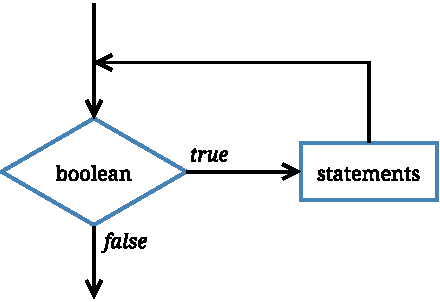
\includegraphics[scale=0.9]{figs/while.pdf}
\caption{Flow of execution for a \java{while} loop.}
\label{fig.while}
\end{center}
\end{figure}

\index{loop body}
\index{infinite loop}
\index{loop!infinite}

The {\bf body} of the loop should change the value of one or more variables so that, eventually, the condition becomes \java{false} and the loop terminates.
Otherwise the loop will repeat forever, which is called an {\bf infinite loop}.

\begin{code}
int n = 3;
while (n > 0) {
    System.out.println(n);
    // n never changes
}
\end{code}

This example will print the number \java{3} forever, or at least until you terminate the program.
An endless source of amusement for computer scientists is the observation that the directions on shampoo, ``Lather, rinse, repeat,'' are an infinite loop.

In the first example, we can prove that the loop terminates when \java{n} is positive.
But in general, it is not so easy to tell whether a loop terminates.
For example, this loop continues until \java{n} is 1 (which makes the condition \java{false}):

\begin{code}
while (n != 1) {
    System.out.println(n);
    if (n % 2 == 0) {         // n is even
        n = n / 2;
    } else {                  // n is odd
        n = 3 * n + 1;
    }
}
\end{code}

Each time through the loop, the program displays the value of \java{n} and then checks whether it is even or odd.
If it is even, the value of \java{n} is divided by two.
If it is odd, the value is replaced by $3n+1$.
For example, if the starting value is 3, the resulting sequence is 3, 10, 5, 16, 8, 4, 2, 1.

Since \java{n} sometimes increases and sometimes decreases, there is no obvious proof that \java{n} will ever reach 1 and that the program will ever terminate.
For some values of \java{n}, such as the powers of two, we can prove that it terminates.
The previous example ends with such a sequence, starting when \java{n} is 16 (or $2^4$).

The hard question is whether this program terminates for {\em all} values of n.
So far, no one has been able to prove it {\em or} disprove it!
For more information, see \url{https://en.wikipedia.org/wiki/Collatz_conjecture}.
%The field of computer science is interested in these types of questions, because their answers give insight to the limits of what computers can and cannot do.


\section{Increment and decrement}

Here is another \java{while} loop example; this one displays the numbers 1 to 5.

\begin{code}
int i = 1;
while (i <= 5) {
    System.out.println(i);
    i++;  // add 1 to i
}
\end{code}

\index{increment}
\index{decrement}

Assignments like \java{i = i + 1} don't often appear in loops, because Java provides a more concise way to add and subtract by one.
Specifically, \java{++} is the {\bf increment} operator; it has the same effect as \java{i = i + 1}.
And \java{--} is the {\bf decrement} operator; it has the same effect as \java{i = i - 1}.

%So far in this book we have only used (\java{=}) to assign values to variables.
%For convenience, Java provides other assignment operators that increase or decrease the value of a variable.

If you want to increment or decrement a variable by an amount other than \java{1}, you can use \java{+=} and \java{-=}.
For example, \java{i += 2} increments \java{i} by \java{2}.

\begin{code}
int i = 2;
while (i <= 8) {
    System.out.print(i + ", ");
    i += 2;  // add 2 to i
}
System.out.println("Who do we appreciate?");
\end{code}

And the output is:

\begin{stdout}
2, 4, 6, 8, Who do we appreciate?
\end{stdout}


\section{The for statement}

\index{for}
\index{loop!for}
\index{statement!for}

The loops we have written so far have several elements in common.
They start by initializing a variable, they have a condition that depends on that variable, and inside the loop they do something to update that variable.

\index{iteration}

Running the same code multiple times is called {\bf iteration}.
This type of loop is so common that there is another statement, the \java{for} loop, that expresses it more concisely.
For example, we can rewrite the 2-4-6-8 loop this way:

\begin{code}
for (int i = 2; i <= 8; i += 2) {
    System.out.print(i + ", ");
}
System.out.println("Who do we appreciate?");
\end{code}

\java{for} loops have three components in parentheses, separated by semicolons: the initializer, the condition, and the update.

\begin{enumerate}

\item The {\em initializer} runs once at the very beginning of the loop.
(It is equivalent to the line before the \java{while} statement.)

\item The {\em condition} is checked each time through the loop.
If it is \java{false}, the loop ends.
Otherwise, the body of the loop is executed (again).

\item At the end of each iteration, the {\em update} runs, and we go back to step~2.

\end{enumerate}

The \java{for} loop is often easier to read because it puts all the loop-related statements at the top of the loop.
Doing so allows you to focus on the statements in the loop body.
Figure~\ref{fig.for} illustrates \java{for} loops with a flowchart.

\begin{figure}[!ht]
\begin{center}
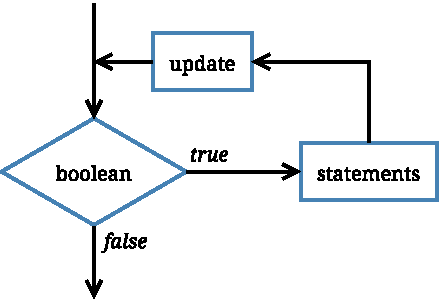
\includegraphics[scale=0.9]{figs/for.pdf}
\caption{Flow of execution for a \java{for} loop.}
\label{fig.for}
\end{center}
\end{figure}

There is another difference between \java{for} loops and \java{while} loops: if you declare a variable in the initializer, it only exists {\em inside} the \java{for} loop.
For example:

\begin{code}
for (int n = 3; n > 0; n--) {
    System.out.println(n);
}
System.out.println("n is now " + n);  // compiler error
\end{code}

The last line tries to display \java{n} (for no reason other than demonstration) but it won't work.
If you need to use a loop variable outside the loop, you have to declare it {\em outside} the loop, like this:

\begin{code}
int n;
for (n = 3; n > 0; n--) {
    System.out.println(n);
}
System.out.println("n is now " + n);
\end{code}

Notice that the \java{for} statement does not say \java{int n = 3}.
Rather, it simply initializes the existing variable \java{n}.


\section{Nested loops}
\label{nested}

Like conditional statements, loops can be nested one inside the other.
Nested loops allow you to iterate over two variables.
For example, we can generate a ``multiplication table'' like this:

\begin{code}
for (int x = 1; x <= 10; x++) {
    for (int y = 1; y <= 10; y++) {
        System.out.printf("%4d", x * y);
    }
    System.out.println();
}
\end{code}

\index{loop variable}
\index{variable!loop}
\index{inner loop}
\index{outer loop}

Variables like \java{x} and \java{y} are called {\bf loop variables}, because they control the execution of a loop.
In this example, the first loop (\java{for x}) is known as the ``outer loop'', and the second loop (\java{for y}) is known as the ``inner loop''.

Each loop repeats their corresponding statements 10 times.
The outer loop iterates from 1 to 10 only once, but the inner loop iterates from 1 to 10 each of those 10 times.
As a result, the \java{printf} method is invoked 100 times.

\index{format specifier}

The format specifier \java{\%4d} displays the value of \java{x * y} padded with spaces so it's four characters wide.
Doing so causes the output to align vertically, regardless of how many digits the numbers have:

\begin{stdout}
   1   2   3   4   5   6   7   8   9  10
   2   4   6   8  10  12  14  16  18  20
   3   6   9  12  15  18  21  24  27  30
   4   8  12  16  20  24  28  32  36  40
   5  10  15  20  25  30  35  40  45  50
   6  12  18  24  30  36  42  48  54  60
   7  14  21  28  35  42  49  56  63  70
   8  16  24  32  40  48  56  64  72  80
   9  18  27  36  45  54  63  72  81  90
  10  20  30  40  50  60  70  80  90 100
\end{stdout}

It's important to realize that the output is displayed row by row.
The inner loop displays a single row of output, followed by a newline.
The outer loop iterates over the rows themselves.
Another way to read nested loops, like the ones in this example, is ``for each row \java{x}, and for each column \java{y}, \ldots''


\section{Characters}

Some of the most interesting problems in computer science involve searching and manipulating text.
In the next few sections, we'll discuss how to apply loops to strings.
Although the examples are short, the techniques work the same whether you have one word or one million words.

\index{charAt}
\index{char}
\index{type!char}

Strings provide a method named \java{charAt}.
It returns a \java{char}, a data type that stores an individual character (as opposed to strings of them).

\begin{code}
String fruit = "banana";
char letter = fruit.charAt(0);
\end{code}

The argument \java{0} means that we want the character at {\bf index} 0.
String indexes range from 0 to $n-1$, where $n$ is the length of the string.
So the character assigned to \java{letter} is \java{b}.

\begin{center}
\ttfamily
\begin{tabular}{cccccc}
\hline
\multicolumn{1}{|l|}{b} & \multicolumn{1}{l|}{a} & \multicolumn{1}{l|}{n} & \multicolumn{1}{l|}{a} & \multicolumn{1}{l|}{n} & \multicolumn{1}{l|}{a} \\ \hline
0                       & 1                      & 2                      & 3                      & 4                      & 5
\end{tabular}
\end{center}


Characters work like the other data types we have seen.
You can compare them using relational operators:

\begin{code}
if (letter == 'a') {
    System.out.println('?');
}
\end{code}

\index{quote mark}
\index{escape sequence}

Character literals, like \java{'a'}, appear in single quotes.
Unlike string literals, which appear in double quotes, character literals can only contain a single character.
Escape sequences, like \java{'\\t'}, are legal because they represent a single character.

The increment and decrement operators also work with characters.
So this loop displays the letters of the alphabet:

\begin{code}
System.out.print("Roman alphabet: ");
for (char c = 'A'; c <= 'Z'; c++) {
    System.out.print(c);
}
System.out.println();
\end{code}

\index{Unicode}

Java uses {\bf Unicode} to represent characters, so strings can store text in other alphabets like Cyrillic and Greek, and non-alphabetic languages like Chinese.
You can read more about it at \url{http://unicode.org/}.

In Unicode, each character is represented by a ``code point'', which you can think of as an integer.
The code points for uppercase Greek letters run from 913 to 937, so we can display the Greek alphabet like this:

\begin{code}
System.out.print("Greek alphabet: ");
for (int i = 913; i <= 937; i++) {
    System.out.print((char) i);
}
System.out.println();
\end{code}

This example uses a type cast to convert each integer (in the range) to the corresponding character.
Try running the code and see what happens.


\section{String iteration}

\index{iteration}

The following loop iterates the characters in \java{fruit} and displays them, one on each line:

\begin{code}
for (int i = 0; i < fruit.length(); i++) {
    char letter = fruit.charAt(i);
    System.out.println(letter);
}
\end{code}

\index{string!length}
\index{length!string}

Strings provide a method called \java{length} that returns the number of characters in the string.
Because it is a method, you have to invoke it with the empty argument list, \java{()}.
When \java{i} is equal to the length of the string, the condition becomes \java{false} and the loop terminates.

To find the last letter of a string, you might be tempted to do something like:

\begin{code}
int length = fruit.length();
char last = fruit.charAt(length);      // wrong!
\end{code}

\index{StringIndexOutOfBoundsException}
\index{exception!StringIndexOutOfBounds}

This code compiles and runs, but invoking the \java{charAt} method throws a \java{StringIndexOutOfBoundsException}.
The problem is that there is no sixth letter in \java{"banana"}.
Since we started counting at 0, the 6 letters are indexed from 0 to 5.
To get the last character, you have to subtract 1 from \java{length}.

\begin{code}
int length = fruit.length();
char last = fruit.charAt(length - 1);  // correct
\end{code}

Many string algorithms involve reading one string and building another.
For example, to reverse a string, we can add one character at a time:

\begin{code}
public static String reverse(String s) {
    String r = "";
    for (int i = s.length() - 1; i >= 0; i--) {
        r += s.charAt(i);
    }
    return r;
}
\end{code}

\index{empty string}

The initial value of \java{r} is \java{""}, which is the {\bf empty string}.
The loop iterates the letters of \java{s} in reverse order.
Each time through the loop, it creates a new string and assigns it to \java{r}.
When the loop exits, \java{r} contains the letters from \java{s} in reverse order.
So the result of \java{reverse("banana")} is \java{"ananab"}.


\section{The indexOf method}

\index{indexOf}

To search for a specific character in a string, you could write a \java{for} loop and use \java{charAt} like in the previous section.
However, the \java{String} class already provides a method for doing just that.

\begin{code}
String fruit = "banana";
int index = fruit.indexOf('a');     // returns 1
\end{code}

This example finds the index of \java{'a'} in the string.
But the letter appears three times, so it's not obvious what \java{indexOf} should do.
According to the documentation, it returns the index of the {\em first} appearance.

To find subsequent appearances, you can use another version of \java{indexOf}, which takes a second argument that indicates where in the string to start looking.

\begin{code}
int index = fruit.indexOf('a', 2);  // returns 3
\end{code}

To visualize how \java{indexOf} and other \java{String} methods work, it helps to draw a picture like Figure~\ref{fig.banana}.
The previous code starts at index 2 (the first \java{'n'}) and finds the next \java{'a'}, which is at index 3.

\begin{figure}[!ht]
\begin{center}
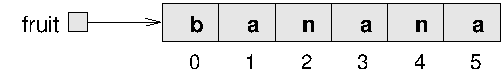
\includegraphics{figs/banana.pdf}
\caption{Memory diagram for a \java{String} of six characters.}
\label{fig.banana}
\end{center}
\end{figure}

%\begin{center}
%\begin{tabular}{c|c|c|c|c|c}
%%\hline
%b & a & n & a & n & a \\
%\hline
%0 & 1 & 2 & 3 & 4 & 5 \\
%%\hline
%\end{tabular}
%\end{center}

If the character happens to appear at the starting index, the starting index is the answer.
So \java{fruit.indexOf('a', 5)} returns \java{5}.
If the character does not appear in the string, \java{indexOf} returns \java{-1}.
Since indexes cannot be negative, this value indicates the character was not found.

You can also use \java{indexOf} to search for an entire string, not just a single character.
For example, the expression \java{fruit.indexOf("nan")} returns \java{2}.


\section{String comparison}
\label{strcmp}

\index{equals}

To compare two strings, it may be tempting to use the \java{==} and \java{!=} operators.

\begin{code}
String name1 = "Alan Turing";
String name2 = "Ada Lovelace";
if (name1 == name2) {                 // wrong!
    System.out.println("The names are the same.");
}
\end{code}

This code compiles and runs, and sometimes it gets the answer right.
But sometimes it gets the answer wrong.
If you give it two different strings that contain the same letters, the condition will be \java{false}.

The problem is that the \java{==} operator checks whether the two variables refer to the {\em same object} by comparing the references.
We'll learn more about references in the next chapter.
The correct way to compare strings is with the \java{equals} method, like this:

\begin{code}
if (name1.equals(name2)) {
    System.out.println("The names are the same.");
}
\end{code}

This example invokes \java{equals} on \java{name1} and passes \java{name2} as an argument.
The \java{equals} method returns \java{true} if the strings contain the same characters; otherwise it returns \java{false}.

\index{compareTo}

If the strings differ, we can use \java{compareTo} to see which comes first in alphabetical order:

\begin{code}
int diff = name1.compareTo(name2);
if (diff == 0) {
    System.out.println("The names are the same.");
} else if (diff < 0) {
    System.out.println("name1 comes before name2.");
} else if (diff > 0) {
    System.out.println("name2 comes before name1.");
}
\end{code}

The return value from \java{compareTo} is the difference between the first characters in the strings that are not the same.
In the preceding code, \java{compareTo} returns positive 8, because the second letter of \java{"Ada"} comes before the second letter of \java{"Alan"} by 8 letters.

If the strings are equal, their difference is zero.
If the first string (the one on which the method is invoked) comes first in the alphabet, the difference is negative.
Otherwise, the difference is positive.

\index{case-sensitive}

Both \java{equals} and \java{compareTo} are case-sensitive.
In Unicode, uppercase letters come before lowercase letters.
So \java{"Ada"} comes before \java{"ada"}.


\section{Substrings}

\index{substring}

The \java{substring} method returns a new string that copies letters from an existing string, starting at the given index.

\begin{itemize}
\item \java{fruit.substring(0)} returns \java{"banana"}
\item \java{fruit.substring(2)} returns \java{"nana"}
\item \java{fruit.substring(6)} returns \java{""}
\end{itemize}

The first example returns a copy of the entire string.
The second example returns all but the first two characters.
As the last example shows, \java{substring} returns the empty string if the argument is the length of the string.

Like most string methods, \java{substring} is overloaded.
That is, there are other versions of \java{substring} that have different parameters.
If it's invoked with two arguments, they are treated as a start and end index:

\begin{itemize}
\item \java{fruit.substring(0, 3)} returns \java{"ban"}
\item \java{fruit.substring(2, 5)} returns \java{"nan"}
\item \java{fruit.substring(6, 6)} returns \java{""}
\end{itemize}

Notice that the character indicated by the end index is {\em not} included.
Defining \java{substring} this way simplifies some common operations.
For example, to select a substring with length \java{len}, starting at index \java{i}, you could write \java{fruit.substring(i, i + len)}.
%So \java{fruit.substring(2, 2 + 3)} returns \java{"nan"}.


\section{String formatting}

\index{printf}

In Section~\ref{printf}, we learned how to use \java{System.out.printf} to display formatted output.
Sometimes programs need to create strings that are formatted a certain way, but not display them immediately, or ever.
For example, the following method returns a time string in 12-hour format:

\begin{code}
public static String timeString(int hour, int minute) {
    String ampm;
    if (hour < 12) {
        ampm = "AM";
        if (hour == 0) {
            hour = 12;  // midnight
        }
    } else {
        ampm = "PM";
        hour = hour - 12;
    }
    return String.format("%02d:%02d %s", hour, minute, ampm);
}
\end{code}

\index{string!format}

\java{String.format} takes the same arguments as \java{System.out.printf}: a format specifier followed by a sequence of values.
The main difference is that \java{System.out.printf} displays the result on the screen.
\java{String.format} creates a new string, but does not display anything.

In this example, the format specifier \java{\%02d} means ``two digit integer padded with zeros'', so \java{timeString(19, 5)} returns the string \java{"07:05 PM"}.
As an exercise, try writing two nested \java{for} loops (in \java{main}) that invoke \java{timeString} and display all possible times over a 24-hour period.

At some point today, skim through the documentation for \java{String}.
Knowing what other methods are there will help you avoid reinventing the wheel.
The easiest way to find documentation for Java classes is to do a web search for ``Java'' and the name of the class.


\section{Vocabulary}

\begin{description}

\term{loop}
A statement that executes a sequence of statements repeatedly.

\term{loop body}
The statements inside the loop.

\term{infinite loop}
A loop whose condition is always true.

\term{increment}
Increase the value of a variable.

\term{decrement}
Decrease the value of a variable.

\term{iteration}
Executing a sequence of statements repeatedly.

\term{loop variable}
A variable that is initialized, tested, and updated in order to control a loop.

\term{index}
An integer variable or value used to indicate a character in a string.

\term{Unicode}
An international standard for representing characters in most of the world's languages.

\term{empty string}
The string \java{""}, which contains no characters and has a length of zero.

\end{description}


\section{Exercises}

The code for this chapter is in the {\tt ch06} directory of {\tt ThinkJavaCode2}.
See page~\pageref{code} for instructions on how to download the repository.
Before you start the exercises, we recommend that you compile and run the examples.

If you have not already read Appendix~\ref{debugger}, now might be a good time.
It describes the DrJava debugger, which is a useful tool for visualizing the flow of execution through loops.


\begin{exercise}  %%V6 Ex7.1

Consider the following methods:

\begin{code}
public static void main(String[] args) {
    loop(10);
}

public static void loop(int n) {
    int i = n;
    while (i > 1) {
        System.out.println(i);
        if (i % 2 == 0) {
            i = i / 2;
        } else {
            i = i + 1;
        }
    }
}
\end{code}

\begin{enumerate}

\item Draw a table that shows the value of the variables \java{i} and \java{n} during the execution of \java{loop}.
The table should contain one column for each variable and one line for each iteration.

\item What is the output of this program?

\item Can you prove that this loop terminates for any positive value of \java{n}?

% If i is odd and we increment by 1, the result is even.  So the second
% branch is always followed by the first branch.
% If i is even and we divide by 2, the result might be odd.  So in the
% worst case, we might alternate between the branches.
% But we can't do more of the second branch than the first.
% So we divide at least as often as we add.

% If i is 1, we're done.
% If i is 2, we divide by 2 and we're done.
% If i is greater than 2, the first branch decreases more than the
% second branch increases.
% So if we do one of each, the net effect is a decrease.
% Therefore, the value of i has to decrease after any two steps.

\end{enumerate}

\end{exercise}


\begin{exercise}  %%V6 Ex7.2

Let's say you are given a number, $a$, and you want to find its square root.
One way to do that is to start with a rough guess about the answer, $x_0$, and then improve the guess using this formula:
%
\[ x_1 =(x_0 + a/x_0) / 2 \]
%
For example, if we want to find the square root of 9, and we start with $x_0 = 6$, then $x_1 = (6 + 9/6) / 2 = 3.75$, which is closer.
We can repeat the procedure, using $x_1$ to calculate $x_2$, and so on.
In this case, $x_2 = 3.075$ and $x_3 = 3.00091$.
So it converges quickly on the correct answer.

Write a method called \java{squareRoot} that takes a \java{double} and returns an approximation of the square root of the parameter, using this technique.
You should not use \java{Math.sqrt}.

As your initial guess, you should use $a/2$.
Your method should iterate until it gets two consecutive estimates that differ by less than 0.0001.
%In other words, return when the absolute value of $x_n - x_{n-1}$ is less than 0.0001.
You can use \java{Math.abs} to calculate the absolute value of the difference.

\end{exercise}


\begin{exercise}  %%V6 Ex7.6

One way to evaluate $\exp(-x^2)$ is to use the infinite series expansion:
%
\[ \exp(-x^2) = 1 - x^2 + x^4/2 - x^6/6 + \ldots \]
%
The $i$th term in this series is $(-1)^i x^{2i} / i!$.
Write a method named \java{gauss} that takes \java{x} and \java{n} as arguments and returns the sum of the first \java{n} terms of the series.
You should not use \java{factorial} or \java{pow}.

\end{exercise}


\begin{exercise}  %%V6 Ex9.5

\index{abecedarian}

A word is said to be ``abecedarian'' if the letters in the word appear in alphabetical order.
For example, the following are all six-letter English abecedarian words:

\begin{quote}
abdest, acknow, acorsy, adempt, adipsy, agnosy, befist, behint, %\\
beknow, bijoux, biopsy, cestuy, chintz, deflux, dehors, dehort, %\\
deinos, diluvy, dimpsy %\\
\end{quote}

Write a method called \java{isAbecedarian} that takes a \java{String} and returns a \java{boolean} indicating whether the word is abecedarian.
%Your method can be iterative or recursive.

\end{exercise}


\begin{exercise}  %%V6 Ex9.6
\label{doubloon}

\index{doubloon}

A word is said to be a ``doubloon'' if every letter that appears in the word appears exactly twice.
Here are some example doubloons found in the dictionary:

\begin{quote}
Abba, Anna, appall, appearer, appeases, arraigning, beriberi, bilabial, boob, Caucasus, coco, Dada, deed, Emmett, Hannah, horseshoer, intestines, Isis, mama, Mimi, murmur, noon, Otto, papa, peep, reappear, redder, sees, Shanghaiings, Toto
\end{quote}

Write a method called \java{isDoubloon} that takes a string and checks whether it is a doubloon.
To ignore case, invoke the \java{toLowerCase} method before checking.
\end{exercise}


\begin{exercise}  %%V6 Ex9.8

\index{Scrabble}

In Scrabble\footnote{Scrabble is a registered trademark owned in the USA and Canada by Hasbro Inc., and in the rest of the world by J.\ W.\ Spear \& Sons Limited of Maidenhead, Berkshire, England, a subsidiary of Mattel Inc.} each player has a set of tiles with letters on them.
The object of the game is to use those letters to spell words.
The scoring system is complex, but longer words are usually worth more than shorter words.

Imagine you are given your set of tiles as a string, like \java{"quijibo"}, and you are given another string to test, like \java{"jib"}.

Write a method called \java{canSpell} that takes two strings and checks whether the set of tiles can spell the word.
You might have more than one tile with the same letter, but you can only use each tile once.

\end{exercise}


\chapter{Arrays and References}

Up to this point, the only variables we have used were for individual values such as numbers or strings.
In this chapter, we'll learn how to store multiple values of the same type using a single variable.
This language feature will enable you to write programs that manipulate larger amounts of data.

For example, Exercise~\ref{doubloon} asked you to check whether every letter in a string appears exactly twice.
One algorithm (which hopefully you already discovered) is to loop through the string 26 times, once for each lowercase letter:

\begin{code}
// outer loop: for each lowercase letter
for (char c = 'a'; c <= 'z'; c++) {
    // inner loop: count how many times the letter appears
    for (int i = 0; i < str.length(); i++) {
        ...
    // if the count is not 0 or 2, return false
\end{code}

This ``nested loops'' approach is inefficient, especially when the string is long.  For example, there are more than 3 million characters in {\it War and Peace}; to process the whole book, the nested loop would run about 80 million times.

Another algorithm would initialize 26 variables to zero, loop through the string {\em one time}, and use a giant \java{if} statement to update the variable for each letter.
But who wants to declare 26 variables?

That's where arrays come in.
We can use a single variable to store 26 integers.
Rather than use an \java{if} statement to update each value, we can use arithmetic to update the $n$th value directly.
We will present this algorithm at the end of the chapter.


\section{Creating Arrays}

\index{array}
\index{element}

An {\bf array} is a sequence of values; the values in the array are called {\bf elements}.
You can make an array of \java{int}s, \java{double}s, \java{String}s, or any other type, but all the values in an array must have the same type.

\index{type!array}
\index{[ ] square brackets}
\index{brackets!square}

To create an array, you have to declare a variable with an {\em array type} and then create the array itself.
Array types look like other Java types, except they are followed by square brackets (\java{[]}).
For example, the following lines declare that \java{counts} is an ``integer array'' and \java{values} is a ``double array'':

\begin{code}
int[] counts;
double[] values;
\end{code}

\index{new}
\index{operator!new}
\index{allocate}

To create the array itself, you have to use the \java{new} operator, which we first saw in Section~\ref{scanner}.
The \java{new} operator {\bf allocates} memory for the array and automatically initializes all of its elements to zero.

\begin{code}
counts = new int[4];
values = new double[size];
\end{code}

The first assignment makes \java{counts} refer to an array of four integers.
The second makes \java{values} refer to an array of \java{double}s, but the number of elements depends on the value of \java{size} (at the time the array is created).

Of course, you can also declare the variable and create the array with a single line of code:

\begin{code}
int[] counts = new int[4];
double[] values = new double[size];
\end{code}

\index{NegativeArraySizeException}
\index{exception!NegativeArraySize}

You can use any integer expression for the size of an array, as long as the value is nonnegative.
If you try to create an array with \java{-4} elements, for example, you will get a \java{NegativeArraySizeException}.
An array with zero elements is allowed, and there are special uses for such arrays.

You can initialize an array with an {\bf array literal}, which is a comma-separated sequence of elements enclosed in braces, like this:

\begin{code}
int[] a = {1, 2, 3, 4};
\end{code}

This statement creates an array variable, \java{a}, and makes it refer to an array with four elements.


\section{Accessing Elements}
\label{elements}

When you create an array with the \java{new} operator, the elements are initialized to zero.
Figure~\ref{fig.array} shows a memory diagram of the \java{counts} array so far.

\begin{figure}[!ht]
\begin{center}
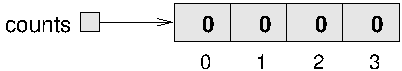
\includegraphics{figs/array.pdf}
\caption{Memory diagram of an \java{int} array.}
\label{fig.array}
\end{center}
\end{figure}

\index{reference}

The arrow indicates that the value of \java{counts} is a {\bf reference} to the array.
You should think of {\em the array} and {\em the variable} that refers to it as two different things.
As we'll soon see, we can assign a different variable to refer to the same array, and we can change the value of \java{counts} to refer to a different array.

\index{element}
\index{index}
\index{array!element}
\index{array!index}

The boldface numbers inside the boxes are the elements of the array.
The lighter numbers outside the boxes are the {\bf indexes} used to identify each location in the array.
As with strings, the index of the first element is 0, not 1.
For this reason, we sometimes refer to the first element as the ``zeroth'' element.

The \java{[]} operator selects elements from an array:

\begin{code}
System.out.println("The zeroth element is " + counts[0]);
\end{code}

You can use the \java{[]} operator anywhere in an expression:

\begin{code}
counts[0] = 7;
counts[1] = counts[0] * 2;
counts[2]++;
counts[3] -= 60;
\end{code}

Figure~\ref{fig.array2} shows the result of these statements.

\begin{figure}[!ht]
\begin{center}
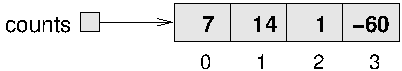
\includegraphics{figs/array2.pdf}
\caption{Memory diagram after several assignment statements.}
\label{fig.array2}
\end{center}
\end{figure}

You can use any expression as an index, as long as it has type \java{int}.
One of the most common ways to index an array is with a loop variable.
For example:

\begin{code}
int i = 0;
while (i < 4) {
    System.out.println(counts[i]);
    i++;
}
\end{code}

This \java{while} loop counts up from 0 to 4.
When \java{i} is 4, the condition fails and the loop terminates.
So the body of the loop is only executed when \java{i} is 0, 1, 2, and 3.
In this context, the variable name \java{i} is short for ``index''.

\index{loop variable}
\index{variable!loop}

Each time through the loop we use \java{i} as an index into the array, displaying the $i$th element.
This type of array processing is usually written as a \java{for} loop.

\begin{code}
for (int i = 0; i < 4; i++) {
    System.out.println(counts[i]);
}
\end{code}

\index{ArrayIndexOutOfBoundsException}
\index{exception!ArrayIndexOutOfBounds}

For the \java{counts} array, the only legal indexes are 0, 1, 2, and 3.
If the index is negative or greater than 3, the result is an \java{ArrayIndexOutOfBoundsException}.


\section{Displaying Arrays}
\label{printarray}

\index{array!printing}

You can use \java{println} to display an array, but it probably doesn't do what you would like.
For example, if you print an array like this:

\begin{code}
int[] a = {1, 2, 3, 4};
System.out.println(a);
\end{code}

The output is something like:

\begin{stdout}
[I@bf3f7e0
\end{stdout}

The bracket indicates that the value is an array, \java{I} stands for ``integer'', and the rest represents the address of the array in memory.

If we want to display the elements of the array, we can do it ourselves:

\begin{code}
public static void printArray(int[] a) {
    System.out.print("{" + a[0]);
    for (int i = 1; i < a.length; i++) {
        System.out.print(", " + a[i]);
    }
    System.out.println("}");
}
\end{code}

Given the previous array, the output of \java{printArray} is:

\begin{stdout}
{1, 2, 3, 4}
\end{stdout}

\index{utility class}
\index{Arrays class}

The Java library includes a class, \java{java.util.Arrays}, that provides methods for working with arrays.
One of them, \java{toString}, returns a string representation of an array.
After importing \java{Arrays}, we can invoke \java{toString} like this:

\begin{code}
System.out.println(Arrays.toString(a));
\end{code}

And the output is:

\begin{stdout}
[1, 2, 3, 4]
\end{stdout}

Notice that \java{Arrays.toString} uses square brackets instead of curly braces.
But it beats writing your own \java{printArray} method.


\section{Copying Arrays}

\index{array!copying}

As explained in Section~\ref{elements}, array variables contain {\em references} to arrays.
When you make an assignment to an array variable, it simply copies the reference.
But it doesn't copy the array itself.
For example:

\begin{code}
double[] a = new double[3];
double[] b = a;
\end{code}

These statements create an array of three \java{double}s and make two different variables refer to it, as shown in Figure~\ref{fig.array3}.

\index{memory diagram}
\index{diagram!memory}

\begin{figure}[!ht]
\begin{center}
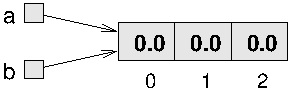
\includegraphics{figs/array3.pdf}
\caption{Memory diagram of two variables referring to the same array.}
\label{fig.array3}
\end{center}
\end{figure}

\index{alias}

Any changes made through either variable will be seen by the other.
For example, if we set \java{a[0] = 17.0}, and then display \java{b[0]}, the result is {\tt 17.0}.
Because \java{a} and \java{b} are different names for the same thing, they are sometimes called {\bf aliases}.

If you actually want to copy the array, not just the reference, you have to create a new array and copy the elements from one to the other, like this:

\begin{code}
double[] b = new double[3];
for (int i = 0; i < 3; i++) {
    b[i] = a[i];
}
\end{code}

\index{Arrays class}

\java{java.util.Arrays} provides a method named \java{copyOf} that performs this task for you.
So you can replace the previous code with one line:

\begin{code}
double[] b = Arrays.copyOf(a, 3);
\end{code}

The second parameter is the number of elements you want to copy, so \java{copyOf} can also be used to copy part of an array.
Figure~\ref{fig.array4} shows the state of the array variables after invoking \java{Arrays.copyOf}.

\begin{figure}[!ht]
\begin{center}
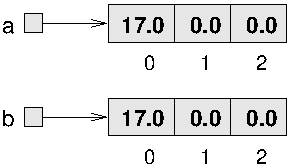
\includegraphics{figs/array4.pdf}
\caption{Memory diagram of two variables referring to different arrays.}
\label{fig.array4}
\end{center}
\end{figure}


%\section{Array Length}

\index{length!array}
\index{array!length}

The examples so far only work if the array has three elements.
It is better to generalize the code to work with arrays of any size.
We can do that by replacing the magic number, \java{3}, with \java{a.length}:

\begin{code}
double[] b = new double[a.length];
for (int i = 0; i < a.length; i++) {
    b[i] = a[i];
}
\end{code}

All arrays have a built-in constant, \java{length}, that stores the number of elements.
In contrast to \java{String.length()}, which is a method, \java{a.length} is a constant.
The expression \java{a.length} may look like a method invocation, but there are no parentheses and no arguments.

The last time the loop gets executed, \java{i} is \java{a.length - 1}, which is the index of the last element.
When \java{i} is equal to \java{a.length}, the condition fails and the body is not executed -- which is a good thing, because trying to access \java{a[a.length]} would throw an exception.

Of course we can replace the loop altogether by using \java{Arrays.copyOf} and \java{a.length} for the second argument.
The following line produces the same result shown in Figure~\ref{fig.array4}.

\begin{code}
double[] b = Arrays.copyOf(a, a.length);
\end{code}

The \java{Arrays} class provides many other useful methods like \java{Arrays.compare}, \java{Arrays.equals}, \java{Arrays.fill}, and \java{Arrays.sort}.
Take a moment to read the documentation by searching the web for \java{java.util.Arrays}.


\section{Array Traversal}
\label{traversal}

\index{traversal}

Many computations can be implemented by looping through the elements of an array and performing an operation on each element.
Looping through the elements of an array is called a {\bf traversal}.

\begin{code}
int[] a = {1, 2, 3, 4, 5};
for (int i = 0; i < a.length; i++) {
    a[i] *= a[i];
}
\end{code}

This example traverses an array and squares each element.
At the end of the loop, the array has the values 
\verb"{1, 4, 9, 16, 25}".

\index{search}

Another common pattern is a {\bf search}, which involves traversing an array and ``searching'' for a particular element.
For example, the following method takes an array and a value, and it returns the index where the value appears:

% TODO: comparing floating point values doesn't always work (credit: Fazl)

\begin{code}
public static int search(double[] array, double target) {
    for (int i = 0; i < array.length; i++) {
        if (array[i] == target) {
            return i;
        }
    }
    return -1;  // not found
}
\end{code}

If we find the target value in the array, we return its index immediately.
If the loop exits without finding the target, it returns \java{-1}, a special value chosen to indicate a failed search.
(This code is essentially what the \java{String.indexOf} method does.)

The following code searches an array for the value \java{1.23}, which is the third element.
Because array indexes start at zero, the output is \java{2}.

\begin{code}
double[] array = {3.14, -55.0, 1.23, -0.8};
int index = search(array, 1.23);
System.out.println(index);
\end{code}


\index{reduce}

Another common traversal is a {\bf reduce} operation, which ``reduces'' an array of values down to a single value.
Examples include the sum or product of the elements, the minimum, and the maximum.
The following method takes an array and returns the sum of its elements:

\begin{code}
public static double sum(double[] array) {
    double total = 0.0;
    for (int i = 0; i < array.length; i++) {
        total += array[i];
    }
    return total;
}
\end{code}

\index{accumulator}

Before the loop, we initialize \java{total} to zero.
Each time through the loop, we update \java{total} by adding one element from the array.
At the end of the loop, \java{total} contains the sum of the elements.
A variable used this way is sometimes called an {\bf accumulator}, because it ``accumulates'' the running total.


\section{Random Numbers}
\label{random}

\index{deterministic}

Most computer programs do the same thing every time they run; programs like that are called {\bf deterministic}.
Usually determinism is a good thing, since we expect the same calculation to yield the same result.
But for some applications, we want the computer to be unpredictable.
Games are an obvious example, but there are many others, like scientific simulations.

%Technically speaking, all computer programs are deterministic: they simply execute the source code.

\index{nondeterministic}
\index{pseudorandom}

Making a program {\bf nondeterministic} turns out to be hard, because it's impossible for a computer to generate truly random numbers.
But there are algorithms that generate unpredictable sequences called {\bf pseudorandom} numbers.
For most applications, they are as good as random.

%Nondeterminism is a theoretical concept for analyzing the complexity of algorithms.

\index{Random}
\index{nextInt!Random}

If you did Exercise~\ref{guess}, you have already seen \java{java.util.Random}, which generates pseudorandom numbers.
The method \java{nextInt} takes an integer argument, \java{n}, and returns a random integer between \java{0} and \java{n - 1} (inclusive).

If you generate a long series of random numbers, every value should appear, at least approximately, the same number of times.
One way to test this behavior of \java{nextInt} is to generate a large number of values, store them in an array, and count the number of times each value occurs.

The following method creates an \java{int} array and fills it with random numbers between 0 and 99.
The argument specifies the desired size of the array, and the return value is a reference to the new array.

\begin{code}
public static int[] randomArray(int size) {
    Random random = new Random();
    int[] a = new int[size];
    for (int i = 0; i < a.length; i++) {
        a[i] = random.nextInt(100);
    }
    return a;
}
\end{code}

The following \java{main} method generates an array and displays it using \java{printArray} from Section~\ref{printarray}.
We could have used \java{Arrays.toString}, but we like seeing curly braces instead of square brackets.

\begin{code}
public static void main(String[] args) {
    int[] array = randomArray(8);
    printArray(array);
}
\end{code}

Each time you run the program, you should get different values.
The output will look something like this:

\begin{stdout}
{15, 62, 46, 74, 67, 52, 51, 10}
\end{stdout}


\section{Building a Histogram}
\label{singlepass}

\index{histogram}
\index{counter}

If these values were exam scores -- and they would be pretty bad exam scores in that case -- the teacher might present them to the class in the form of a {\bf histogram}.
In statistics, a histogram is a set of counters that keeps track of the number of times each value appears.

For exam scores, we might have ten counters to keep track of how many students scored in the 90s, the 80s, etc.
To do that, we can traverse the array and count the number of elements that fall in a given range.

The following method takes an array and two integers.
It returns the number of elements that fall in the range from \java{low} to \java{high - 1}.

\begin{code}
public static int inRange(int[] a, int low, int high) {
    int count = 0;
    for (int i = 0; i < a.length; i++) {
        if (a[i] >= low && a[i] < high) {
            count++;
        }
    }
    return count;
}
\end{code}

\index{reduce}

This pattern should look familiar: it is another reduce operation.
Notice that \java{low} is included in the range (\java{>=}), but \java{high} is excluded (\java{<}).
This design keeps us from counting any scores twice.

Now we can count the number of scores in each grade range.
We add the following code to our \java{main} method:

\begin{code}
int[] scores = randomArray(30);
int a = inRange(scores, 90, 100);
int b = inRange(scores, 80, 90);
int c = inRange(scores, 70, 80);
int d = inRange(scores, 60, 70);
int f = inRange(scores, 0, 60);
\end{code}

This code is repetitive, but it is acceptable as long as the number of ranges is small.
Suppose we wanted to keep track of the number of times each individual score appears.
Then we would have to write 100 lines of code:

\begin{code}
int count0 = inRange(scores, 0, 1);
int count1 = inRange(scores, 1, 2);
int count2 = inRange(scores, 2, 3);
...
int count99 = inRange(scores, 99, 100);
\end{code}

What we need is a way to store 100 counters, preferably so we can use an index to access them.
Wait a minute, that's exactly what an array does.

The following fragment creates an array of 100 counters, one for each possible score.
It loops through the scores and uses \java{inRange} to count how many times each score appears.
Then it stores the results in the \java{counts} array:

\begin{code}
int[] counts = new int[100];
for (int i = 0; i < counts.length; i++) {
    counts[i] = inRange(scores, i, i + 1);
}
\end{code}

Notice that we are using the loop variable \java{i} three times: as an index into the \java{counts} array, and in the last two arguments of \java{inRange}.

\index{efficiency}

The code works, but it is not as efficient as it could be.
Every time the loop invokes \java{inRange}, it traverses the entire array.
It would be better to make a single pass through the \java{scores} array.

For each score, we already know which range it falls in -- the score itself.
We can use that value to increment the corresponding counter.
This code traverses the array of scores {\em only once} to generate the histogram:

\begin{code}
int[] counts = new int[100];
for (int i = 0; i < scores.length; i++) {
    int index = scores[i];
    counts[index]++;
}
\end{code}

Each time through the loop, it selects one element from \java{scores} and uses it as an index to increment the corresponding element of \java{counts}.
Because this code traverses the array of scores only once, it is much more efficient.


\section{The Enhanced for Loop}
\label{enhanced}

Since traversing arrays is so common, Java provides an alternative syntax that makes the code more compact.
Consider a \java{for} loop that displays the elements of an array on separate lines:

\begin{code}
for (int i = 0; i < values.length; i++) {
    int value = values[i];
    System.out.println(value);
}
\end{code}

We could rewrite the loop like this:

\begin{code}
for (int value : values) {
    System.out.println(value);
}
\end{code}

\index{enhanced for loop}
\index{for!enhanced}

This statement is called an {\bf enhanced for loop}, also known as the ``for each'' loop.
You can read the code as, ``for each \java{value} in \java{values}''.
It's conventional to use plural nouns for array variables and singular nouns for element variables.

Notice how the single line \java{for (int value : values)} replaces the first two lines of the standard \java{for} loop.
It hides the details of iterating each index of the array, and instead, focuses on the values themselves.

Using the enhanced \java{for} loop, and removing the temporary variable, we can write the histogram code from the previous section more concisely:

\begin{code}
int[] counts = new int[100];
for (int score : scores) {
    counts[score]++;
}
\end{code}

Enhanced \java{for} loops often make the code more readable, especially for accumulating values.
But they are not helpful when you need to refer to the index, as in search operations.

\begin{code}
for (double d : array) {
    if (d == target) {
        // array contains d, but we don't know where
    }
}
\end{code}


\section{Counting Characters}

We now return to the example from the beginning of the chapter and present a solution to Exercise~\ref{doubloon} using arrays.
Here is the problem again:

\begin{quote}
A word is said to be a ``doubloon'' if every letter that appears in the word appears exactly twice.
Write a method called \java{isDoubloon} that takes a string and checks whether it is a doubloon.
To ignore case, invoke the \java{toLowerCase} method before checking.
\end{quote}

Based on the approach from Section~\ref{singlepass}, we will create an array of 26 integers to count how many times each letter appears.
We convert the string to lowercase, so that we can treat \java{'A'} and \java{'a'} (for example) as the same latter.

\begin{code}
int[] counts = new int[26];
String lower = s.toLowerCase();
\end{code}

We can use a \java{for} loop to iterate each character in the string.
To update the \java{counts} array, we need to compute the index that corresponds to each character.
Fortunately, Java allows you to perform arithmetic on characters.

\begin{code}
for (int i = 0; i < lower.length(); i++) {
    char letter = lower.charAt(i);
    int index = letter - 'a';
    counts[index]++;
}
\end{code}

If \java{letter} is \java{'a'}, the value of \java{index} is \java{0};
if \java{letter} is \java{'b'}, the value of \java{index} is \java{1},
and so on.

Then we use \java{index} to increment the corresponding element of \java{counts}.
At the end of the loop, \java{counts} contains a histogram of the letters in the string \java{lower}.

\index{toCharArray}

We can simplify this code with an enhanced \java{for} loop, but it doesn't work with strings; we have to convert \java{lower} to an array of characters, like this:

\begin{code}
for (char letter : lower.toCharArray()) {
    int index = letter - 'a';
    counts[index]++;
}
\end{code}

Once we have the counts, we can use a second \java{for} loop to check whether each letter appears 0 or 2 times.

\begin{code}
for (int count : counts) {
    if (count != 0 && count != 2) {
        return false;  // not a doubloon
    }
}
return true;  // is a doubloon
\end{code}

If we find a count that is neither 0 or 2, we know the word is not a doubloon and we can return immediately.
If we make it all the way through the \java{for} loop, we know that all counts are 0 or 2, which means the word is a doubloon.

Pulling together the code fragments, and adding some comments and test cases, here's the entire program.

\index{Doubloon.java}

\begin{trinket}{Doubloon.java}
public class Doubloon {

    public static boolean isDoubloon(String s) {
        // count the number of times each letter appears
        int[] counts = new int[26];
        String lower = s.toLowerCase();
        for (char letter : lower.toCharArray()) {
            int index = letter - 'a';
            counts[index]++;
        }
        // determine whether the given word is a doubloon
        for (int count : counts) {
            if (count != 0 && count != 2) {
                return false;
            }
        }
        return true;
    }

    public static void main(String[] args) {
        System.out.println(isDoubloon("Mama"));  // true
        System.out.println(isDoubloon("Lama"));  // false
    }
}
\end{trinket}

% ABD: Nice test cases :)

This example uses methods, \java{if} statements, \java{for} loops, arithmetic and logical operators, integers, characters, strings, booleans, and arrays.
We hope you'll take a second to appreciate how much you've learned!

%TODO: Switch to em dashes with no spaces.  Sure would be easier if the book were in one file :(
%CSM: That's what wildcards are for :)


\section{Vocabulary}

\begin{description}

\term{array}
A collection of values, where all the values have the same type, and each value is identified by an index.

\term{element}
One of the values in an array.
The \java{[]} operator selects elements.

\term{index}
An integer variable or value used to indicate an element of an array.

\term{allocate}
To reserve memory for an array or other object.
In Java, the \java{new} operator allocates memory.

\term{reference}
A value that indicates a storage location.
In a memory diagram, a reference appears as an arrow.

\term{alias}
A variable that refers to the same object as another variable.

\term{traversal}
Looping through the elements of an array (or other collection).

\term{search}
A traversal pattern used to find a particular element of an array.

\term{reduce}
A traversal pattern that combines the elements of an array into a single value.

\term{accumulator}
A variable used to accumulate results during a traversal.

\term{deterministic}
A program that does the same thing every time it is run.

\term{nondeterministic}
A program that always behaves differently, even when run multiple times with the same input.

\term{pseudorandom}
A sequence of numbers that appear to be random, but which are actually the product of a deterministic computation.

\term{histogram}
An array of integers where each integer counts the number of values that fall into a certain range.

\term{enhanced for loop}
An alternative syntax for traversing the elements of an array (or other collection).

\end{description}


\section{Exercises}

The code for this chapter is in the {\tt ch07} directory of {\tt ThinkJavaCode2}.
See page~\pageref{code} for instructions on how to download the repository.
Before you start the exercises, we recommend that you compile and run the examples.

If you haven't already, take a look at Appendix~\ref{debugging} where we've collected some of our favorite debugging advice.
It refers to language features we haven't yet covered, but it's good for you to know what's available when you need it.


\begin{exercise}  %%V6 Ex8.2

The purpose of this exercise is to practice reading code and recognizing the traversal patterns in this chapter.
The following methods are hard to read, because instead of using meaningful names for the variables and methods, they use names of fruit.

For each method, write one sentence that describes what the method does, without getting into the details of how it works.
And for each variable, identify the role it plays.

\begin{code}
public static int banana(int[] a) {
    int kiwi = 1;
    int i = 0;
    while (i < a.length) {
        kiwi = kiwi * a[i];
        i++;
    }
    return kiwi;
}
\end{code}

\begin{code}
public static int grapefruit(int[] a, int grape) {
    for (int i = 0; i < a.length; i++) {
        if (a[i] == grape) {
            return i;
        }
    }
    return -1;
}
\end{code}

\begin{code}
public static int pineapple(int[] a, int apple) {
    int pear = 0;
    for (int pine: a) {
        if (pine == apple) {
            pear++;
        }
    }
    return pear;
}
\end{code}

\end{exercise}


\begin{exercise}  %%V6 Ex8.3

What is the output of the following program?
Describe in a few words what \java{mus} does.
Draw a stack diagram just before \java{mus} returns.
%that shows the state of the program

\begin{code}
public static int[] make(int n) {
    int[] a = new int[n];
    for (int i = 0; i < n; i++) {
        a[i] = i + 1;
    }
    return a;
}
\end{code}

\begin{code}
public static void dub(int[] jub) {
    for (int i = 0; i < jub.length; i++) {
        jub[i] *= 2;
    }
}
\end{code}

\begin{code}
public static int mus(int[] zoo) {
    int fus = 0;
    for (int i = 0; i < zoo.length; i++) {
        fus += zoo[i];
    }
    return fus;
}
\end{code}

\begin{code}
public static void main(String[] args) {
    int[] bob = make(5);
    dub(bob);
    System.out.println(mus(bob));
}
\end{code}

\end{exercise}


\begin{exercise}  %%V6 Ex8.4

Write a method called \java{indexOfMax} that takes an array of integers and returns the index of the largest element.
Can you write this method using an enhanced \java{for} loop?
Why or why not?

\end{exercise}


\begin{exercise}  %%V6 Ex8.5

The Sieve of Eratosthenes is ``a simple, ancient algorithm for finding all prime numbers up to any given limit,'' which you can read about at \url{https://en.wikipedia.org/wiki/Sieve_of_Eratosthenes}.

Write a method called \java{sieve} that takes an integer parameter, \java{n}, and returns a \java{boolean} array that indicates, for each number from \java{0} to \java{n - 1}, whether the number is prime.

\end{exercise}


\begin{exercise}  %%V6 Ex8.6

Write a method named \java{areFactors} that takes an integer \java{n} and an array of integers, and that returns \java{true} if the numbers in the array are all factors of \java{n} (which is to say that \java{n} is divisible by all of them).

\end{exercise}


\begin{exercise}  %%V6 Ex8.7

Write a method named \java{arePrimeFactors} that takes an integer \java{n} and an array of integers, and that returns \java{true} if the numbers in the array are all prime {\it and} their product is \java{n}.

\end{exercise}


\begin{exercise}  %%V6 Ex9.2

Write a method called \java{letterHist} that takes a string as a parameter and returns a histogram of the letters in the string.
The zeroth element of the histogram should contain the number of a's in the string (upper- and lowercase); the 25th element should contain the number of z's.
Your solution should only traverse the string once.

\end{exercise}


\begin{exercise}  %%V6 Ex9.7

\index{anagram}

Two words are anagrams if they contain the same letters and the same number of each letter.
For example, ``stop'' is an anagram of ``pots'', ``allen downey'' is an anagram of ``well annoyed'', and ``christopher mayfield'' is an anagram of ``hi prof the camel is dry''.
Write a method that takes two strings and checks whether they are anagrams of each other.

\end{exercise}


\chapter{Recursive Methods}

\index{iterative}
\index{recursive}

Up to this point, we've been using \java{while} and \java{for} loops whenever we've needed to repeat something.
Methods that use iteration are called {\bf iterative}.
They are straight-forward, but sometimes there are more elegant solutions.

In this chapter, we explore one of the most magical things that a method can do: invoke {\em itself} to solve a smaller version of the {\em same} problem.
A method that invokes itself is called {\bf recursive}.


\section{Recursive Void Methods}
\label{recursion}

\index{countdown}

Consider the following example:

\begin{code}
public static void countdown(int n) {
    if (n == 0) {
        System.out.println("Blastoff!");
    } else {
        System.out.println(n);
        countdown(n - 1);
    }
}
\end{code}

The name of the method is \java{countdown}; it takes a single integer as a parameter.
If the parameter is zero, it displays the word ``Blastoff''.
Otherwise, it displays the number and then invokes itself, passing \java{n - 1} as the argument.

What happens if we invoke \java{countdown(3)} from \java{main}?

\vspace{-1ex}
\begin{quote}
The execution of \java{countdown} begins with \java{n == 3}, and since \java{n} is not zero, it displays the value 3, and then invokes itself...
\begin{quote}
The execution of \java{countdown} begins with \java{n == 2}, and since \java{n} is not zero, it displays the value 2, and then invokes itself...
\begin{quote}
The execution of \java{countdown} begins with \java{n == 1}, and since \java{n} is not zero, it displays the value 1, and then invokes itself...
\begin{quote}
The execution of \java{countdown} begins with \java{n == 0}, and since \java{n} is zero, it displays the word ``Blastoff!'' and then returns.
\end{quote}
The \java{countdown} that got \java{n == 1} returns.
\end{quote}
The \java{countdown} that got \java{n == 2} returns.
\end{quote}
The \java{countdown} that got \java{n == 3} returns.
\end{quote}
\vspace{-1ex}

And then you're back in \java{main}.
So the total output looks like:

\begin{stdout}
3
2
1
Blastoff!
\end{stdout}

As a second example, we'll rewrite the methods \java{newLine} and \java{threeLine} from Section~\ref{adding_methods}.
Here they are again:

\begin{code}
public static void newLine() {
    System.out.println();
}

public static void threeLine() {
    newLine();
    newLine();
    newLine();
}
\end{code}

\index{newline}

Although these methods work, they would not help if we wanted to display two newlines, or maybe 100.
A more general alternative would be:

\begin{code}
public static void nLines(int n) {
    if (n > 0) {
        System.out.println();
        nLines(n - 1);
    }
}
\end{code}

This method takes an integer, \java{n}, as a parameter and displays \java{n} newlines.
The structure is similar to \java{countdown}.
As long as $n$ is greater than zero, it displays a newline and then invokes itself to display $(n-1)$ additional newlines.
The total number of newlines is $1 + (n - 1)$, which is just what we wanted: $n$.


\section{Recursive Stack Diagrams}

\index{stack diagram}
\index{diagram!stack}

In Section~\ref{stack}, we used a stack diagram to represent the state of a program during a method invocation.
The same kind of diagram can make it easier to interpret a recursive method.

Remember that every time a method gets called, Java creates a new frame that contains the method's parameters and variables.
Figure~\ref{fig.stack2} is a stack diagram for \java{countdown}, called with \java{n == 3}.

\begin{figure}[!ht]
\begin{center}
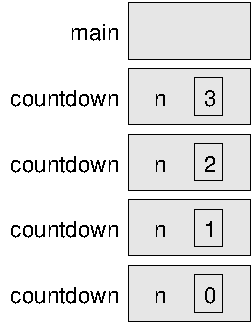
\includegraphics{figs/stack2.pdf}
\caption{Stack diagram for the \java{countdown} program.}
\label{fig.stack2}
\end{center}
\end{figure}

By convention, the frame for \java{main} is at the top, and the stack of other frames grows down.
That way, we can draw stack diagrams on paper without needing to guess how far they will grow.
The frame for \java{main} is empty because \java{main} does not have any variables.
(It has the parameter \java{args}, but since we're not using it, we left it out of the diagram.)

\index{base case}

There are four frames for \java{countdown}, each with a different value for the parameter \java{n}.
The last frame, with \java{n == 0}, is called the {\bf base case}.
It does not make a recursive call, so there are no more frames below it.

\index{StackOverflowError}
\index{exception!StackOverflow}

If there is no base case in a recursive method, or if the base case is never reached, the stack would grow forever---at least in theory.
In practice, the size of the stack is limited.
If you exceed the limit, you get a \java{StackOverflowError}.

For example, here is a recursive method without a base case:

\begin{code}
public static void forever(String s) {
    System.out.println(s);
    forever(s);
}
\end{code}

\index{call stack}

This method displays the given string until the stack overflows, at which point it throws an error.
Try this example on your computer---you might be surprised by how long the error message is!


\section{Value-Returning Methods}
\label{factorial}

%\index{Turing complete}
%\index{language!complete}
%
%\index{Turing, Alan}
%\index{Church, Alonzo}
%
%Now that we have methods that return values, we have a {\bf Turing complete} programming language.
%That means Java can compute anything computable, for any reasonable definition of ``computable''.
%This idea was developed by Alonzo Church and Alan Turing, so it is known as the Church-Turing thesis.
%You can read more about it at \url{https://en.wikipedia.org/wiki/Turing_thesis}.

To give you an idea of what you can do with the tools we have learned, let's look at methods that evaluate recursively-defined mathematical functions.

A recursive definition is similar to a ``circular'' definition, in the sense that the definition refers to the thing being defined.
Of course, a truly circular definition is not very useful:

\begin{quote}
{\bf recursive:} \\
An adjective used to describe a method that is recursive.
\end{quote}

\index{recursion}

If you saw that definition in the dictionary, you might be annoyed.
Then again, if you search for ``recursion'' on Google, it displays ``Did you mean: recursion'' as an inside joke.
People fall for that link all the time.

\index{factorial}

Many mathematical functions are defined recursively, because that is often the simplest way.
For example, the {\bf factorial} of an integer $n$, which is written $n!$, is defined like this:
%
\begin{eqnarray*}
&&  0! = 1 \\
&&  n! = n \cdot(n-1)!
\end{eqnarray*}
%
Don't confuse the mathematical symbol $!$, which means {\em factorial}, with the Java operator \java{!}, which means {\em not}.
This definition says that \java{factorial(0)} is \java{1}, and \java{factorial(n)} is \java{n * factorial(n - 1)}.

So \java{factorial(3)} is \java{3 * factorial(2)}; \java{factorial(2)} is \java{2 * factorial(1)}; \java{factorial(1)} is \java{1 * factorial(0)}; and \java{factorial(0)} is \java{1}.
Putting it all together, we get \java{3 * 2 * 1 * 1}, which is 6.

If you can formulate a recursive definition of something, you can easily write a Java method to evaluate it.
The first step is to decide what the parameters and return type are.
Since factorial is defined for integers, the method takes an \java{int} as a parameter and returns an \java{int}.
%So here's a good starting place:

\begin{code}
public static int factorial(int n) {
    return 0;  // stub
}
\end{code}

Next, we think about the base case.
If the argument happens to be zero, we return 1.

\begin{code}
public static int factorial(int n) {
    if (n == 0) {
        return 1;
    }
    return 0;  // stub
}
\end{code}

Otherwise, and this is the interesting part, we have to make a recursive call to find the factorial of $n-1$, and then multiply it by $n$.

\begin{code}
public static int factorial(int n) {
    if (n == 0) {
        return 1;
    }
    int recurse = factorial(n - 1);
    int result = n * recurse;
    return result;
}
\end{code}

To illustrate what is happening, we'll use the temporary variables \java{recurse} and \java{result}.
In each method call, \java{recurse} stores the factorial of $n - 1$, and \java{result} stores the factorial of $n$.

The flow of execution for this program is similar to \java{countdown} from Section~\ref{recursion}.
If we invoke \java{factorial} with the value 3:

\vspace{-1ex}
\begin{quote}
Since 3 is not zero, we skip the first branch and calculate the factorial of $n-1$...
\begin{quote}
Since 2 is not zero, we skip the first branch and calculate the factorial of $n-1$...
\begin{quote}
Since 1 is not zero, we skip the first branch and calculate the factorial of $n-1$...
\begin{quote}
Since 0 {\em is} zero, we take the first branch and return the value 1 immediately.
% without making any more recursive invocations.
\end{quote}
The return value (1) gets multiplied by \java{n}, which is 1, and the result is returned.
\end{quote}
The return value (1) gets multiplied by \java{n}, which is 2, and the result is returned.
\end{quote}
The return value (2) gets multiplied by \java{n}, which is 3, and the result, 6, is returned to whatever invoked \java{factorial(3)}.
\end{quote}
\vspace{-1ex}

\index{stack diagram}
\index{diagram!stack}

Figure~\ref{fig.stack3} shows what the stack diagram looks like for this sequence of method invocations.
The return values are shown being passed up the stack.
Notice that \java{recurse} and \java{result} do not exist in the last frame, because when \java{n == 0} the code that declares them does not execute.

\begin{figure}[!ht]
\begin{center}
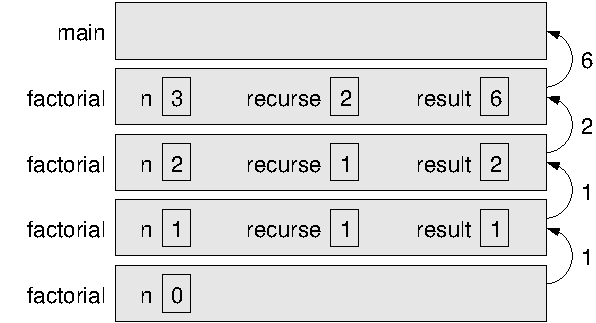
\includegraphics{figs/stack3.pdf}
\caption{Stack diagram for the \java{factorial} method.}
\label{fig.stack3}
\end{center}
\end{figure}


\section{The Leap of Faith}
\label{leap_of_faith}

\index{leap of faith}

Following the flow of execution is one way to read programs, but it can quickly become overwhelming.
Another way to understand recursion is the {\bf leap of faith}:
when you come to a method invocation, instead of following the flow of execution, you {\em assume} that the method works correctly and returns the appropriate value.

In fact, you are already practicing this leap of faith when you use methods in the Java library.
When you invoke \java{Math.cos} or \java{System.out.println}, you don't think about the implementations of those methods.
You just assume that they work properly.

The same is true of other methods.
For example, consider the method from Section~\ref{boolmeth} that determines whether an integer has only one digit:

\begin{code}
public static boolean isSingleDigit(int x) {
    return x > -10 && x < 10;
}
\end{code}

Once you convince yourself that this method is correct---by examining and testing the code---you can just use the method without ever looking at the implementation again.

Recursive methods are no different.
When you get to a recursive call, don't think about the flow of execution.
Instead, {\em assume} that the recursive call produces the desired result.

For example, ``Assuming that I can find the factorial of $n-1$, can I compute the factorial of $n$?''
Yes you can, by multiplying by $n$.
Here's an implementation of \java{factorial} with the temporary variables removed:

\begin{code}
public static int factorial(int n) {
    if (n == 0) {
        return 1;
    }
    return n * factorial(n - 1);
}
\end{code}

Notice how similar this version is to the original mathematical definition:
%There is essentially a one-to-one correspondence.
%
\begin{eqnarray*}
&&  0! = 1 \\
&&  n! = n \cdot(n-1)!
\end{eqnarray*}
%
Of course, it is strange to assume that the method works correctly when you have not finished writing it.
But that's why it's called a leap of faith!


%\section{Fibonacci Sequence}
\label{fibonacci}

\index{fibonacci}

Another common recursively-defined mathematical function is the Fibonacci sequence, which has the following definition:
%
\begin{eqnarray*}
&& fibonacci(1) = 1 \\
&& fibonacci(2) = 1 \\
&& fibonacci(n) = fibonacci(n-1) + fibonacci(n-2)
\end{eqnarray*}
%
Notice that each Fibonacci number is the sum of the two preceding Fibonacci numbers.
Translated into Java, this function is:

\begin{code}
public static int fibonacci(int n) {
    if (n == 1 || n == 2) {
        return 1;
    }
    return fibonacci(n - 1) + fibonacci(n - 2);
}
\end{code}

If you try to follow the flow of execution here, even for small values of \java{n}, your head will explode.
But if we take a leap of faith and assume that the two recursive invocations work correctly, then it is clear, looking at the definition, that our implementation is correct.


\section{Counting Up Recursively}
\label{countup}

The \java{countdown} example in Section~\ref{recursion} has three parts: (1) it checks the base case, (2) it displays something, and (3) it makes a recursive call.
What do you think happens if you reverse steps (2) and (3), making the recursive call {\em before} displaying?

\begin{code}
public static void countup(int n) {
    if (n == 0) {
        System.out.println("Blastoff!");
    } else {
        countup(n - 1);
        System.out.println(n);
    }
}
\end{code}

The stack diagram is the same as before, and the method is still called $n$ times.
But now the \java{System.out.println} happens just before each recursive call returns.
As a result, it counts {\em up} instead of down:

\begin{stdout}
Blastoff!
1
2
3
\end{stdout}

Keep this in mind for the next example, which displays numbers in binary.

\section{Binary Number System}
\label{binary}

You are probably aware that computers can only store 1's and 0's.
That's because processors and memory are made up of billions of tiny on-off switches.

The value 1 means a switch is on; the value 0 means a switch is off.
All types of data, whether integer, floating-point, text, audio, video, or something else, are represented by 1's and 0's.

\index{binary}

Fortunately, we can represent any integer as a {\bf binary} number.
The following table shows the first eight numbers in binary and decimal.

\begin{table}[!ht]
\begin{center}
\begin{tabular}{|c|c|}
\hline
Binary & Decimal \\
\hline
0 & 0 \\
\hline
1 & 1 \\
\hline
10 & 2 \\
\hline
11 & 3 \\
\hline
100 & 4 \\
\hline
101 & 5 \\
\hline
110 & 6 \\
\hline
111 & 7 \\
\hline
\end{tabular}
\caption{The first eight binary numbers.}
\label{tab:binary}
\end{center}
\end{table}

%In the decimal system, each part of a number is referred to as a %``digit''.
%For example, the number 456 has three digits.
%In the binary system, each part of a number is referred to as a ``bit''.
%The number 10111 in binary has five bits.

%When you hear the phrase ``64-bit computer'', it means that the %processors and memory use 64 bits to store integers.
%That is where the limits for data types like \java{int} and \java{long} %come from.

% ABD: I think we can leave bits out of the discussion, and just talk
% about different written representations of the same number.

In decimal there are 10 digits, and the written representation of numbers is based on powers of 10.
For example, the number 456 has 4 in the 100's place, 5 in the 10's place, and 6 in the 1's place.
So the value is 400 + 50 + 6.

\begin{center}
\begin{tabular}{|c|c|c|}
\hline
4 & 5 & 6 \\
\hline
$10^2$ & $10^1$ & $10^0$ \\
\hline
\end{tabular}
\end{center}

In binary there are 2 digits, and the written representation of numbers is based on powers of 2.
For example, the number 10111 has 1 in the 16's place, 0 in the 8's place, 1 in the 4's place, 1 in the 2's place, and 1 in the 16's place.
So the value is 16 + 0 + 4 + 2 + 1, which is 23 in decimal.

\begin{center}
\begin{tabular}{|c|c|c|c|c|}
\hline
1 & 0 & 1 & 1 & 1 \\
\hline
$2^4$ & $2^3$ & $2^2$ & $2^1$ & $2^0$ \\
\hline
\end{tabular}
\end{center}

To get the digits of a decimal number, we can use repeated division.
For example, if we divide 456 by 10, we get 45 with remainder 6.
The remainder is the rightmost digit of 456.

If we divide the result again, we get 4 with remainder 5.
The remainder is the second rightmost digit of 456.
And if we divide again, we get 0 with remainder 4.
The remainder is the third rightmost digit of 456, and the result, 0, tells us that we're done.

We can do the same thing in binary if we divide by two.
When you divide by two, the remainder is the right-most digit, either 0 or 1.
If you divide the result again, you get the second rightmost digit.
If you keep going, and write down the remainders, you'll have your number in binary.

\begin{stdout}
23 / 2 is 11 remainder 1
11 / 2 is  5 remainder 1
 5 / 2 is  2 remainder 1
 2 / 2 is  1 remainder 0
 1 / 2 is  0 remainder 1
\end{stdout}

Reading these remainders from bottom to top, 23 in binary is 10111.


\section{Recursive Binary Method}

Now, to display a number in binary we can combine the algorithm from the previous section and the ``count up'' pattern from Section~\ref{countup}.

Here is a recursive method that displays any positive integer in binary:

\begin{code}
public static void displayBinary(int value) {
    if (value > 0) {
        displayBinary(value / 2);
        System.out.print(value % 2);
    }
}
\end{code}

If \java{value} is zero, \java{displayBinary} does nothing (that's the base case).
If the argument is positive, the method divides it by two and calls \java{displayBinary} recursively.
When the recursive call returns, the method displays one digit of the result and returns (again).
Figure~\ref{fig.stack4} illustrates this process.

\index{stack diagram}
\index{diagram!stack}

\begin{figure}[!ht]
\begin{center}
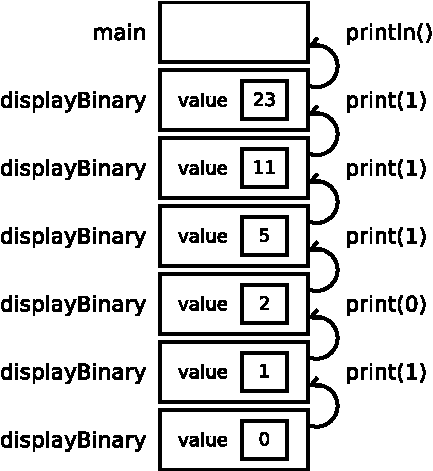
\includegraphics[width=190pt]{figs/stack4.pdf}
\caption{Stack diagram for the \java{displayBinary} method.}
\label{fig.stack4}
\end{center}
\end{figure}

The leftmost digit is near the bottom of the stack, so it gets displayed first.
The rightmost digit, near the top of the stack, gets displayed last.
After invoking \java{displayBinary}, we use \java{println} to complete the output.

\begin{code}
displayBinary(23);      // output is 10111
System.out.println();
\end{code}


\section{CodingBat Problems}

In the past several chapters you've seen methods, conditions, loops, strings, arrays, and recursion.
A great resource for practicing all of these concepts is \url{https://codingbat.com/}.

\index{CodingBat}

{\it CodingBat} is a free website of programming problems developed by Nick Parlante, a Computer Science lecturer at Stanford University.
As you work on these problems, CodingBat saves your progress (if you create an account).

To conclude this chapter, we consider two problems in the {\sf Recursion-1} section of CodingBat.
One of them deals with strings, and the other deals with arrays.
Both of them have the same recursive idea: check the base case, look at the current index, and recursively handle the rest.

The first problem is available at \url{https://codingbat.com/prob/p118230}:

\begin{quote}
\textbf{Recursion-1 ~noX}

Given a string, compute recursively a new string where all the \java{'x'} chars have been removed.

\ttfamily
noX("xaxb") $\rightarrow$ "ab" \\
noX("abc") $\rightarrow$ "abc" \\
noX("xx") $\rightarrow$ ""
\end{quote}

When solving recursive problems, it helps to think about the base case first.
The base case is the easiest version of the problem; for \java{noX}, it's the empty string.
If the argument is an empty string, there are no {\tt x}'s to be removed.

\begin{code}
if (str.length() == 0) {
    return "";
}
\end{code}

% NOTE: Some people like isEmpty(), but I think this is the right
% idiom for our purposes
% https://www.techiedelight.com/check-string-empty-or-null-java/

Next comes the more difficult part.
To solve a problem recursively, you need to think of a simpler instance of the same problem.
For \java{noX}, it's removing all the {\tt x}'s from a shorter string.

So let's split the string into two parts, the first letter and the rest.

\begin{code}
char first = str.charAt(0);
String rest = str.substring(1);
\end{code}

Now we can make a recursive call to remove the {\tt x}'s from {\tt rest}:

\begin{code}
String recurse = noX(rest);
\end{code}

If {\tt first} happens to be an {\tt x}, we're done; we just have to return {\tt recurse}.
Otherwise, we have to concatenate {\tt first} and {\tt recurse}.
Here's the \java{if} statement we need.

\begin{code}
if (first == 'x') {
    return recurse;
} else {
    return first + recurse;
}
\end{code}

You can run this solution on CodingBat by pasting these snippets into the provided method definition.

The second problem is available at \url{https://codingbat.com/prob/p135988}:

\begin{quote}
\textbf{Recursion-1 ~array11}

Given an array of ints, compute recursively the number of times that the value 11 appears in the array.

\ttfamily
array11([1, 2, 11], 0) $\rightarrow$ 1 \\
array11([11, 11], 0) $\rightarrow$ 2 \\
array11([1, 2, 3, 4], 0) $\rightarrow$ 0
\end{quote}

This problem uses the convention of passing the index as an argument.
So the base case is when we've reached the end of the array.
At that point, we know there are no more {\tt 11}'s.

\begin{code}
if (index >= nums.length) {
    return 0;
}
\end{code}

Next we look at the current number (based on the given index), and check if it's an {\tt 11}.
After that, we can recursively check the rest of the array.
Similar to the noX problem, we look at only one integer per method call.

\begin{code}
int recurse = array11(nums, index + 1);
if (nums[index] == 11) {
    return recurse + 1;
} else {
    return recurse;
}
\end{code}

Again, you can run this solutions on CodingBat by pasting the snippets into the method definition.

\index{Java Tutor}

To see how these solutions actually work, you might find it helpful to step through them with a debugger (see Appendix~\ref{debugger}) or Java Tutor (\url{https://thinkjava.org/javatutor}).
Then try solving other CodingBat problems on your own.

Learning to think recursively is an important part of learning to think like a computer scientist.
Many algorithms can be written concisely with recursive methods that perform computations on the way down, on the way up, or both.


\section{Vocabulary}

\begin{description}

%\term{void method}
%A method that does not return a value.

%\term{value method}
%A method that returns a value.

\term{iterative}
A method or algorithm that repeats steps using one or more loops.

\term{recursive}
A method or algorithm that invokes itself one or more times with different arguments.

%\term{recursion}
%The process of invoking (and restarting) the same method that is currently executing.

\term{base case}
A condition that causes a recursive method {\em not} to make another recursive call.

%\term{Turing complete}
%A programming language that can implement any theoretically possible algorithm.

\term{factorial}
The product of all the integers up to and including a given integer.

\term{leap of faith}
A way to read recursive programs by assuming that the recursive call works, rather than following the flow of execution.

\term{binary}
A system that uses only zeros and ones to represent numbers.
Also known as ``base 2''.

\end{description}


\section{Exercises}

The code for this chapter is in the {\it ch08} directory of {\it ThinkJavaCode2}.
See page~\pageref{code} for instructions on how to download the repository.
Before you start the exercises, we recommend that you compile and run the examples.

If you have not already read Appendix~\ref{JUnit}, now might be a good time.
It describes JUnit, a standard framework for writing test code.


\begin{exercise}  %%V6 Ex5.5

The purpose of this exercise is to take a problem and break it into smaller problems, and to solve the smaller problems by writing simple methods.
Consider the first verse of the song ``99 Bottles of Beer'':

\begin{quote}
99 bottles of beer on the wall,\\
99 bottles of beer,\\
ya' take one down, ya' pass it around,\\
98 bottles of beer on the wall.
\end{quote}

Subsequent verses are identical except that the number of bottles gets smaller by one in each verse, until the last verse:

\begin{quote}
No bottles of beer on the wall,\\
no bottles of beer,\\
ya' can't take one down, ya' can't pass it around,\\
'cause there are no more bottles of beer on the wall!
\end{quote}

And then the song (finally) ends.

Write a program that displays the entire lyrics of ``99 Bottles of Beer''.
Your program should include a recursive method that does the hard part, but you might want to write additional methods to separate other parts of the program.
As you develop your code, test it with a small number of verses, like \java{3}.

\end{exercise}


\begin{exercise}  %%V6 Ex6.7

Write a recursive method named \java{oddSum} that takes a positive odd integer \java{n} and returns the sum of odd integers from 1 to n.
Start with a base case, and use temporary variables to debug your solution.
You might find it helpful to print the value of \java{n} each time \java{oddSum} is invoked.

\end{exercise}


\begin{exercise}  %%V6 Ex6.6

In this exercise, you will use a stack diagram to understand the execution of the following recursive method.

\begin{code}
public static void main(String[] args) {
    System.out.println(prod(1, 4));
}

public static int prod(int m, int n) {
    if (m == n) {
        return n;
    } else {
        int recurse = prod(m, n - 1);
        int result = n * recurse;
        return result;
    }
}
\end{code}

\begin{enumerate}

\item Draw a stack diagram showing the state of the program just before the last invocation of \java{prod} completes.

\item What is the output of this program?
(Try to answer this question on paper first, then run the code to check your answer.)

\item Explain in a few words what \java{prod} does (without getting into the details of how it works).

\item Rewrite \java{prod} without the temporary variables \java{recurse} and \java{result}.
%
{\em Hint:} You only need one line for the \java{else} branch.

\end{enumerate}

\end{exercise}


\begin{exercise}  %%V6 Ex6.8

The goal of this exercise is to translate a recursive definition into a Java method.
The Ackermann function is defined for non-negative integers as follows:
\begin{eqnarray*}
A(m, n) = \begin{cases}
              n+1 & \mbox{if } m = 0 \\
        A(m-1, 1) & \mbox{if } m > 0 \mbox{ and } n = 0 \\
A(m-1, A(m, n-1)) & \mbox{if } m > 0 \mbox{ and } n > 0
\end{cases}
\end{eqnarray*}

Write a recursive method called \java{ack} that takes two \java{int}s as parameters and that computes and returns the value of the Ackermann function.

Test your implementation of Ackermann by invoking it from \java{main} and displaying the return value.
Note the return value gets very big very quickly.
You should try it only for small values of $m$ and $n$ (not bigger than 3).

\end{exercise}


\begin{exercise}  %%V6 Ex6.9
\label{ex.power}

Write a recursive method called \java{power} that takes a double \java{x} and an integer \java{n} and returns $x^n$.

{\em Hint:} A recursive definition of this operation is $x^n = x \cdot x^{n-1}$.
Also, remember that anything raised to the zeroth power is 1.

Optional challenge: you can make this method more efficient, when \java{n} is even, using $x^n = \left( x^{n/2} \right)^2$.

\end{exercise}


\begin{exercise}  %%V6 Ex8.8

Many of the patterns we have seen for traversing arrays can also be written recursively.
It is not common, but it is a useful exercise.

\begin{enumerate}

\item Write a method called \java{maxInRange} that takes an array of integers and two indexes, \java{lowIndex} and \java{highIndex}, and finds the maximum value in the array, but only considering the elements between \java{lowIndex} and \java{highIndex}, including both.

This method should be recursive.
If the length of the range is 1, that is, if \java{lowIndex == highIndex}, we know immediately that the sole element in the range must be the maximum.
So that's the base case.

If there is more than one element in the range, we can break the array into two pieces, find the maximum in each of the pieces, and then find the maximum of the maxima.

\item Methods like \java{maxInRange} can be awkward to use.
To find the largest element in an array, we have to provide the range for the entire array.

\begin{code}
double max = maxInRange(a, 0, a.length - 1);
\end{code}

Write a method called \java{max} that takes an array and uses \java{maxInRange} to find and return the largest element.

\end{enumerate}

\end{exercise}


\newpage
\begin{exercise}  %%V6 Ex9.4

Create a program called {\it Recurse.java} and type in the following methods:

\begin{code}
/**
 * Returns the first character of the given String.
 */
public static char first(String s) {
    return s.charAt(0);
}
\end{code}

\begin{code}
/**
 * Returns all but the first letter of the given String.
 */
public static String rest(String s) {
    return s.substring(1);
}
\end{code}

\begin{code}
/**
 * Returns all but the first and last letter of the String.
 */
public static String middle(String s) {
    return s.substring(1, s.length() - 1);
}
\end{code}

\begin{code}
/**
 * Returns the length of the given String.
 */
public static int length(String s) {
    return s.length();
}
\end{code}

\begin{enumerate}

\item Write some code in \java{main} that tests each of these methods.
Make sure they work, and you understand what they do.

\item Using these methods, and without using any other \java{String} methods, write a method called \java{printString} that takes a string as a parameter and that displays the letters of the string, one on each line.
It should be a void method.

\item Again using only these methods, write a method called \java{printBackward} that does the same thing as \java{printString} but that displays the string backward (again, one character per line).

\item Now write a method called \java{reverseString} that takes a string as a parameter and that returns a new string as a return value.
The new string should contain the same letters as the parameter, but in reverse order.

\begin{code}
String backwards = reverseString("coffee");
System.out.println(backwards);
\end{code}

The output of this example code should be:

\begin{stdout}
eeffoc
\end{stdout}

\index{palindrome}

\item A palindrome is a word that reads the same both forward and backward, like ``otto'' and ``palindromeemordnilap''.
Here's one way to test whether a string is a palindrome:

\begin{quotation}
\noindent
A single letter is a palindrome, a two-letter word is a palindrome if the letters are the same, and any other word is a palindrome if the first letter is the same as the last and the middle is a palindrome.
\end{quotation}

Write a recursive method named \java{isPalindrome} that takes a \java{String} and returns a \java{boolean} indicating whether the word is a palindrome.

\end{enumerate}

\end{exercise}


%~ \part{Object-Oriented Programming}

\chapter{Immutable Objects}
\label{immutable}

\index{object-oriented}

Java is an ``object-oriented'' language, which means that it uses objects to (1)~represent data and (2)~provide methods related to them.
This way of organizing programs is a powerful design concept, and we will introduce it gradually throughout the remainder of the book.

\index{object}
\index{System.in}
\index{System.out}

An {\bf object} is a collection of data that provides a set of methods.
For example, \java{Scanner}, which we saw in Section~\ref{scanner}, is an object that provides methods for parsing input.
\java{System.out} and \java{System.in} are also objects.

Strings are objects, too.
They contain characters and provide methods for manipulating character data.
Other data types, like \java{Integer}, contain numbers and provide methods for manipulating number data.
We will explore some of these methods in this chapter.


\section{Primitives vs Objects}

\index{primitive}

Not everything in Java is an object: \java{int}, \java{double}, \java{char}, and \java{boolean} are examples of {\bf primitive} types.
%We will explain some of the differences between object types and primitive types as we go along.
When you declare a variable with a primitive type, Java reserves a small amount of memory to store its value.
Figure~\ref{fig.mem1} shows how the following values are stored memory.

\begin{code}
int number = -2;
char symbol = '!';
\end{code}

\begin{figure}[!ht]
\begin{center}
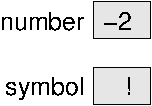
\includegraphics[width=80pt]{figs/mem1.pdf}
\caption{Memory diagram of two primitive variables.}
\label{fig.mem1}
\end{center}
\end{figure}

\index{memory diagram}
\index{diagram!memory}

As we learned in Section~\ref{elements}, an array variable stores a {\em reference} to an array.
That's because the array itself is too large to fit in the variable's memory.
For example, \java{char[] array = \{'c', 'a', 't'\};} contains three characters.

\begin{figure}[!ht]
\begin{center}
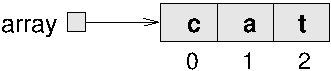
\includegraphics[width=205pt]{figs/mem2.pdf}
\caption{Memory diagram of an array of characters.}
\label{fig.mem2}
\end{center}
\end{figure}

When drawing memory diagrams, we use an arrow to represent the location of the array, as in Figure~\ref{fig.mem2}.
The actual memory location (the {\em value} of the array variable) is an integer chosen by Java at run-time.

Objects work in a similar way.
When you declare an object variable, it will store a reference to an object.
In contrast to arrays, which store multiple elements of the same data type, objects can be used to {\bf encapsulate} any type of data.
%We will learn more about this concept in Chapter~\ref{mutable}.

For example, a \java{String} object encapsulates a character array.
Figure~\ref{fig.mem3} illustrates how strings are stored in memory.

\begin{figure}[!ht]
\begin{center}
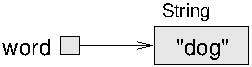
\includegraphics[width=325pt]{figs/mem3.pdf}
\caption{Memory diagram of a \java{String} object.}
\label{fig.mem3}
\end{center}
\end{figure}

Behind the scenes, the code \java{String word = "dog";} creates an array of the characters \java{'d'}, \java{'o'}, and \java{'g'}, and stores the reference to that array in a \java{String} object.
The variable \java{word} contains a reference to the \java{String} object.

\index{string!comparing}

To test whether two integers (or other primitive types) are equal, you simply use the \java{==} operator.
But as we learned in Section~\ref{strcmp}, you need to use the \java{equals} method to compare strings.
The \java{equals} method traverses the arrays and tests whether they contain the same characters.

On the other hand, two \java{String} objects with the same characters would not be considered equal in the \java{==} sense.
The \java{==} operator, when applied to string variables, only tests whether they refer to the {\em same} object.

Objects and arrays are typically created with the \java{new} keyword, which allocates memory for them (see Section~\ref{allocate}).
For convenience, you don't have to use \java{new} when creating strings:

\begin{code}
String word = new String("dog");  // creates a string object
String word = "dog";   // implicitly creates a string object
\end{code}


\section{The null Keyword}

\index{null}

In Java, the keyword \java{null} is a special value that means ``no object''.
You can initialize object and array variables this way:

\begin{code}
String name = null;
int[] combo = null;
\end{code}

The value \java{null} is represented in memory diagrams by a small box with no arrow, as in Figure~\ref{fig.mem4}.
In other words, the variables do not reference anything.

\begin{figure}[!ht]
\begin{center}
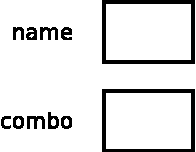
\includegraphics[width=80pt]{figs/mem4.pdf}
\caption{Memory diagram showing variables that are \java{null}.}
\label{fig.mem4}
\end{center}
\end{figure}

\index{NullPointerException}
\index{exception!NullPointer}

If you try to use a variable that is \java{null} by invoking a method or accessing an element, Java throws a \java{NullPointerException}.

\begin{code}
System.out.println(name.length());  // NullPointerException
System.out.println(combo[0]);       // NullPointerException
\end{code}

On the other hand, it is perfectly fine to pass a \java{null} reference as an argument to a method, or to receive one as a return value.
In these situations, \java{null} is often used to represent a special condition or indicate an error.


\section{Strings are Immutable}

If the Java library didn't have a \java{String} class, we would have to use character arrays to store and manipulate text.
Operations like concatenation (\java{+}), \java{indexOf}, and \java{substring} would be difficult and inconvenient.
Fortunately, Java does have a \java{String} class that provides these and other methods.

\index{toUpperCase}
\index{toLowerCase}
\index{immutable}

For example, the methods \java{toLowerCase} and \java{toUpperCase} convert uppercase letters to lowercase, and vice versa.
These methods are often a source of confusion, because it sounds like they modify strings.
But neither these methods nor any others can change a string, because strings are {\bf immutable}.

When you invoke \java{toUpperCase} on a string, you get another \java{String} object as a result.
For example:

\begin{code}
String name = "Alan Turing";
String upperName = name.toUpperCase();
\end{code}

%\index{Turing, Alan}

After these statements run, \java{upperName} refers to the string \java{"ALAN TURING"}.
But \java{name} still refers to \java{"Alan Turing"}.
A common mistake is to assume that \java{toUpperCase} somehow affects the original string:

\begin{code}
String name = "Alan Turing";
name.toUpperCase();           // ignores the return value
System.out.println(name);
\end{code}

The previous code displays \java{"Alan Turing"}, because the value of \java{name} (i.e., the reference to the original \java{String} object) never changes.
If you want to change \java{name} to be uppercase, then you need to assign the return value to it:

\begin{code}
String name = "Alan Turing";
name = name.toUpperCase();    // references the new string
System.out.println(name);
\end{code}

\index{replace}

A similar method is \java{replace}, which finds and replaces instances of one string within another.
This example replaces \java{"Computer Science"} with \java{"CS"}:

\begin{code}
String text = "Computer Science is fun!";
text = text.replace("Computer Science", "CS");
\end{code}

%This example demonstrates a common way to work with string methods.
%It invokes \java{text.replace}, which returns a reference to a new string, \java{"CS is fun!"}.
%Then it assigns the new string to \java{text}, replacing the old string.

As with \java{toUpperCase}, assigning the return value (to \java{text}) is important.
If you don't assign the return value, invoking \java{text.replace} has no effect.

% ABD: Too many new ideas here: the most important one is that you have to do something with the return value. It's not a good time to appreciate the glory of immutability.
% CSM: Now that strings were introduced previously, I would like to make this chapter say more about immutability. But we won't get to the full glory until the next chapter.

Strings are immutable by design, because it simplifies passing them between methods as parameters and return values.
And since the contents of a string can never change, two variables can reference the same string without one accidentally corrupting the other.


\section{Wrapper Classes}

Primitive values (like \java{int}s, \java{double}s, and \java{char}s) cannot be \java{null}, and they do not provide methods.
For example, you can't invoke \java{equals} on an \java{int}:

\begin{code}
int i = 5;
System.out.println(i.equals(5));  // compiler error
\end{code}

\index{wrapper class}
\index{class!wrapper}
\index{Character}
\index{Integer}
\index{Double}

But for each primitive type, there is a corresponding {\bf wrapper class} in the Java library.
The wrapper class for \java{int} is named \java{Integer}, with a capital \java{I}.

\begin{code}
Integer i = new Integer(5);
System.out.println(i.equals(5));  // displays true
\end{code}

Other wrapper classes include \java{Boolean}, \java{Character}, \java{Double}, and \java{Long}.
They are in the \java{java.lang} package, so you can use them without importing them.

Like strings, objects from wrapper classes are immutable.
And you need to use the \java{equals} method to compare them.

\begin{code}
Integer x = new Integer(123);
Integer y = new Integer(123);
if (x == y) {                     // false
    System.out.println("x and y are the same object");
}
if (x.equals(y)) {                // true
    System.out.println("x and y have the same value");
}
\end{code}

Because \java{x} and \java{y} refer to different \java{Integer} objects, the code only displays ``x and y have the same value''.

Each wrapper class defines the constants \java{MIN_VALUE} and \java{MAX_VALUE}.
For example, \java{Integer.MIN_VALUE} is \java{-2147483648}, and \java{Integer.MAX_VALUE} is \java{2147483647}.
Because these constants are available in wrapper classes, you don't have to remember them, and you don't have to write them yourself.

\index{parse}

Wrapper classes also provide methods for converting strings to and from primitive types.
For example, \java{Integer.parseInt} converts a string to (you guessed it) an integer.
In this context, {\bf parse} means ``read and translate''.

\begin{code}
String str = "12345";
int num = Integer.parseInt(str);
\end{code}

The other wrapper classes provide similar methods, like \java{Double.parseDouble} and \java{Boolean.parseBoolean}.
They also provide \java{toString}, which returns a string representation of a value:

\begin{code}
int num = 12345;
String str = Integer.toString(num);
\end{code}

The result is the string \java{"12345"}, which as you now understand, is stored internally in a character array \java{\{'1', '2', '3', '4', '5'\}}.

\index{NumberFormatException}
\index{exception!NumberFormat}

It's always possible to convert a primitive value to a string, but not the other way around.
The following code throws a \java{NumberFormatException}.

\begin{code}
String str = "five";
int num = Integer.parseInt(str);  // NumberFormatException
\end{code}


\section{Command-Line Arguments}

\index{args}
\index{command-line interface}

Now that you know about strings, arrays, and wrapper classes, we can {\em finally} explain the \java{args} parameter of the \java{main} method, which we have been ignoring since Chapter~\ref{theway}.
If you are unfamiliar with the command-line interface, please read Appendix~\ref{commandline}.

Let's write a program to find the maximum value in a sequence of numbers.
Rather than read the numbers from \java{System.in} using a \java{Scanner}, we'll pass them as command-line arguments.
Here is a starting point:

\begin{code}
import java.util.Arrays;
public class Max {
    public static void main(String[] args) {
        System.out.println(Arrays.toString(args));
    }
}
\end{code}

You can run this program from the command line by typing:

\begin{stdout}
java Max
\end{stdout}

\index{empty array}

The output indicates that \java{args} is an {\bf empty array}; that is, it has no elements:

\begin{stdout}
[]
\end{stdout}

If you provide additional values on the command line, they are passed as arguments to \java{main}.
For example, if you run the program like this:

\begin{stdout}
java Max 10 -3 55 0 14
\end{stdout}

The output is:

\begin{stdout}
[10, -3, 55, 0, 14]
\end{stdout}

It's not clear from the output, but the elements of \java{args} are strings.
So \java{args} is the array \java{\{"10", "-3", "55", "0", "14"\}}.
To find the maximum number, we have to convert the arguments to integers.

The following code uses an enhanced \java{for} loop to parse the arguments (using the \java{Integer} wrapper class) and find the largest value:

\begin{code}
int max = Integer.MIN_VALUE;
for (String arg : args) {
    int value = Integer.parseInt(arg);
    if (value > max) {
        max = value;
    }
}
System.out.println("The max is " + max);
\end{code}

We begin by initializing \java{max} to the smallest (most negative) number an \java{int} can represent.
That way, the first value we parse will replace \java{max}.
As we find larger values, they will replace \java{max} as well.

If \java{args} is empty, the result will be \java{MIN_VALUE}.
We can prevent this situation from happening by checking \java{args} at the beginning of the program:

\begin{code}
if (args.length == 0) {
    System.err.println("Usage: java Max <numbers>");
    return;
}
\end{code}

It's customary for programs that require command-line arguments to display a ``usage'' message when there are no arguments given.
For example, if you run {\tt javac} or {\tt java} from the command line without any arguments, you will get a very long message.


\section{BigInteger Arithmetic}
% CSM based on text from V6 Exercise 10.4

It might not be clear at this point why you would ever need an integer object when you can just use an \java{int} or \java{long}.
One advantage is the variety of methods that \java{Integer} and \java{Long} provide.
But there is another reason: when you need very large integers that exceed \java{Long.MAX_VALUE}.

\index{BigInteger}

\java{BigInteger} is a Java class that can represent arbitrarily large integers.
There is no upper bound except the limitations of memory size and processing speed.
Take a minute to read the documentation, which you can find by doing a web search for ``Java BigInteger''.

\index{java.math}

To use BigIntegers, you have to \java{import java.math.BigInteger} at the beginning of your program.
There are several ways to create a BigInteger, but the simplest uses \java{valueOf}.
The following code converts a \java{long} to a BigInteger:

\begin{code}
long x = 17;
BigInteger big = BigInteger.valueOf(x);
\end{code}

You can also create BigIntegers from strings.
For example, here is a 20-digit integer that is too big to store using a \java{long}.

\begin{code}
String s = "12345678901234567890";
BigInteger bigger = new BigInteger(s);
\end{code}

Notice the difference in the previous two examples: you use \java{valueOf} to convert integers, and \java{new BigInteger} to convert strings.

Since BigIntegers are not primitive types, the usual math operators don't work.
Instead, we have to use methods like \java{add}.
To add two BigIntegers, we invoke \java{add} on one and pass the other as an argument.

\begin{code}
BigInteger a = BigInteger.valueOf(17);
BigInteger b = BigInteger.valueOf(1700000000);
BigInteger c = a.add(b);
\end{code}

Like strings, \java{BigInteger} objects are immutable.
Methods like \java{add}, \java{multiply}, and \java{pow} all return new BigIntegers, rather than modify an existing one.

Internally, a BigInteger encapsulates an array of \java{int}s, similar to the way a string encapsulates an array of \java{char}s.
Each \java{int} in the array stores a portion of the BigInteger.
The methods of \java{BigInteger} traverse this array to perform addition, multiplication, etc.

For very long floating-point values, take a look at \java{java.math.BigDecimal}.
Interestingly, \java{BigDecimal} objects represent floating-point numbers internally by encapsulating a \java{BigInteger}!


\section{Program Development}
\label{encapsulation}

This chapter introduces two main concepts: objects encapsulate other types of data, and they can be designed to be immutable.
Applying these concepts helps us to manage the complexity of programs as they become large.

\index{design process}
\index{encapsulation!and generalization}

%Unfortunately, computer science has a lot of overloaded terms.
Another use of the term ``encapsulation'' applies to methods.
In this section, we present a {\bf design process} called ``encapsulation and generalization''.

One challenge of programming, especially for beginners, is figuring out how to divide up a program into methods.
The process of encapsulation and generalization allows you to design as you go along.
The steps are:

\begin{enumerate}
\item Write a few lines of code in \java{main} or another method, and test them.
\item When they are working, wrap them in a new method, and test again.
\item If it's appropriate, replace literal values with variables and parameters.
\end{enumerate}

Encapsulation and generalization is similar to ``incremental development'' (see Section~\ref{distance}), in the sense that you write a little code, test it, and repeat.
But you don't need to begin with an exact method definition and stub.

\index{table!two-dimensional}

To demonstrate this process, we'll develop methods that display multiplication tables.
We begin by writing and testing a few lines of code.
Here is a loop that displays the multiples of two, all on one line:

\begin{code}
for (int i = 1; i <= 6; i++) {
    System.out.printf("%4d", 2 * i);
}
System.out.println();
\end{code}

%\index{loop variable}
%\index{variable!loop}
%
%The first line initializes a variable named \java{i}, which is going to act as the loop variable.
%As the loop executes, the value of \java{i} increases from 1 to 6; when \java{i} is 7, the loop terminates.

Each time through the loop, we display the value \java{2 * i} padded with spaces so it's four characters wide.
Since we use \java{System.out.printf}, the output appears on a single line.

After the loop, we call \java{println} to print a newline character.
Remember that in some environments, none of the output is displayed until the line is complete.
The output of the code so far is:

\begin{stdout}
   2   4   6   8  10  12
\end{stdout}

\index{encapsulate}

The next step is to {\bf encapsulate} (or ``wrap'') this code in a method:

\begin{code}
public static void printRow() {
    for (int i = 1; i <= 6; i++) {
        System.out.printf("%4d", 2 * i);
    }
    System.out.println();
}
\end{code}

\index{generalize}

Finally, we {\bf generalize} the method to print multiples of other numbers by replacing the constant value \java{2} with a parameter \java{n}.
This step is called ``generalization'' because it makes the method more general (less specific).

\begin{code}
public static void printRow(int n) {
    for (int i = 1; i <= 6; i++) {
        System.out.printf("%4d", n * i);  // generalized n
    }
    System.out.println();
}
\end{code}

Invoking this method with the argument \java{2} yields the same output as before.
With the argument \java{3}, the output is:

\begin{stdout}
   3   6   9  12  15  18
\end{stdout}

%And with argument 4, the output is:
%
%\begin{stdout}
%   4   8  12  16  20  24
%\end{stdout}

By now you can probably guess how we are going to display a multiplication table: we'll invoke \java{printRow} repeatedly with different arguments.
In fact, we'll use another loop to iterate through the rows.

\begin{code}
for (int i = 1; i <= 6; i++) {
    printRow(i);
}
\end{code}

And the output looks like this:

\begin{stdout}
   1   2   3   4   5   6
   2   4   6   8  10  12
   3   6   9  12  15  18
   4   8  12  16  20  24
   5  10  15  20  25  30
   6  12  18  24  30  36
\end{stdout}

%The format specifier \java{\%4d} in \java{printRow} causes the output to align vertically, regardless of whether the numbers are one or two digits.


\section{More Generalization}

The previous result is similar to the ``nested loops'' approach in Section~\ref{nested}.
However, the inner loop is now encapsulated in the \java{printRow} method.
We can encapsulate the outer loop in a method too:

\begin{code}
public static void printTable() {
    for (int i = 1; i <= 6; i++) {
        printRow(i);
    }
}
\end{code}

The initial version of \java{printTable} always displays six rows.
We can generalize it by replacing the literal \java{6} with a parameter:

\begin{code}
public static void printTable(int rows) {
    for (int i = 1; i <= rows; i++) {     // generalized rows
        printRow(i);
    }
}
\end{code}

Here is the output of \java{printTable(7)}:

\begin{stdout}
   1   2   3   4   5   6
   2   4   6   8  10  12
   3   6   9  12  15  18
   4   8  12  16  20  24
   5  10  15  20  25  30
   6  12  18  24  30  36
   7  14  21  28  35  42
\end{stdout}

That's better, but it always displays the same number of columns.
We can generalize more by adding a parameter to \java{printRow}:

\begin{code}
public static void printRow(int n, int cols) {
    for (int i = 1; i <= cols; i++) {     // generalized cols
        System.out.printf("%4d", n * i);
    }
    System.out.println();
}
\end{code}

Now \java{printRow} takes two parameters: \java{n} is the value whose multiples should be displayed, and \java{cols} is the number of columns.
Since we added a parameter to \java{printRow}, we also have to change the line in \java{printTable} where it is invoked:

\begin{code}
public static void printTable(int rows) {
    for (int i = 1; i <= rows; i++) {
        printRow(i, rows);                // rows becomes cols
    }
}
\end{code}

When this line executes, it evaluates \java{rows} and passes the value, which is 7 in this example, as an argument.
In \java{printRow}, this value is assigned to \java{cols}.
As a result, the number of columns equals the number of rows, so we get a square 7x7 table (instead of the previous 7x6 table):

%\begin{stdout}
%   1   2   3   4   5   6   7
%   2   4   6   8  10  12  14
%   3   6   9  12  15  18  21
%   4   8  12  16  20  24  28
%   5  10  15  20  25  30  35
%   6  12  18  24  30  36  42
%   7  14  21  28  35  42  49
%\end{stdout}

When you generalize a method appropriately, you often find that it has capabilities you did not plan.
For example, you might notice that the multiplication table is symmetric.
Since $ab = ba$, all the entries in the table appear twice.
You could save ink by printing half of the table, and you would only have to change {\em one line} of \java{printTable}:

\begin{code}
printRow(i, i);  // using i for both n and cols
\end{code}

In English, the length of each row is the same as its row number.
The result is a triangular multiplication table.

\begin{stdout}
   1
   2   4
   3   6   9
   4   8  12  16
   5  10  15  20  25
   6  12  18  24  30  36
   7  14  21  28  35  42  49
\end{stdout}

Generalization makes code more versatile, more likely to be reused, and sometimes easier to write.
In this example, we started with a simple idea and ended with two general-purpose methods.

%Even though the second parameter in \java{printRow} is named \java{size} and we have a variable with the same name, we can still use any value or expression we want for the argument.

%Remember, you do not pass {\em variables} to methods; you pass their current {\em values}.
%In this last example, the value of \java{i} in \java{printTable} is assigned to both \java{n} and \java{cols} in \java{printRow}.


\section{Vocabulary}

\begin{description}

\term{object}
A collection of related data that comes with a set of methods that operate on the data.

\term{primitive}
A data type that stores a single value and provides no methods.

\term{immutable}
An object that, once created, cannot be modified.
Strings are immutable by design.

\term{wrapper class}
Classes in \java{java.lang} that provide constants and methods for working with primitive types.

\term{parse}
To read a string and interpret or translate it.

\term{empty array}
An array with no elements and a length of zero.

\term{design process}
A process for determining what methods a class or program should have.
%So far we have seen ``incremental development'' and ``encapsulation and generalization''.

\term{encapsulate}
To wrap data inside of an object, or to wrap statements inside of a method.

\term{generalize}
To replace something unnecessarily specific (like a constant value) with something appropriately general (like a variable or parameter).

\end{description}


\section{Exercises}

The code for this chapter is in the {\tt ch09} directory of {\tt ThinkJavaCode2}.
See page~\pageref{code} for instructions on how to download the repository.
Before you start the exercises, we recommend that you compile and run the examples.


\begin{exercise}  %%V6 Ex9.1

The point of this exercise is to explore Java types and fill in some of the details that aren't covered in the chapter.

\index{concatenate}

\begin{enumerate}

\item Create a new program named {\tt Test.java} and write a \java{main} method that contains expressions that combine various types using the \java{+} operator.
For example, what happens when you ``add'' a \java{String} and a \java{char}?
Does it perform character addition or string concatenation?
What is the type of the result?
(How can you determine the type of the result?)

\item Make a bigger copy of the following table and fill it in.
At the intersection of each pair of types, you should indicate whether it is legal to use the \java{+} operator with these types, what operation is performed (addition or concatenation), and what the type of the result is.

\begin{center}
\begin{tabular}{|l|l|l|l|l|l|} \hline
        &  boolean  &  ~char~  &  ~~int~~  &  double  &  String \\ \hline
boolean &           &          &           &          &         \\ \hline
char    &           &          &           &          &         \\ \hline
int     &           &          &           &          &         \\ \hline
double  &           &          &           &          &         \\ \hline
String  &           &          &           &          &         \\ \hline
\end{tabular}
\end{center}

\item Think about some of the choices the designers of Java made, based on this table.
How many of the entries seem unavoidable, as if there was no other choice?
How many seem like arbitrary choices from several equally reasonable possibilities?
Which entries seem most problematic?

\item Here's a puzzler: normally, the statement \java{x++} is exactly equivalent to \java{x = x + 1}.
But if \java{x} is a \java{char}, it's not exactly the same!
In that case, \java{x++} is legal, but \java{x = x + 1} causes an error.
Try it out and see what the error message is, then see if you can figure out what is going on.

\item What happens when you add \java{""} (the empty string) to the other types, for example, \java{"" + 5}?

%\item For each data type, what types of values can you assign to it?
%For example, you can assign an \java{int} to a \java{double} but not vice versa.

\end{enumerate}

\end{exercise}


\begin{exercise}  %%V6 Ex8.1

The goal of this exercise is to practice encapsulation and generalization using some of the examples in previous chapters.

\begin{enumerate}

\item Starting with the code in Section~\ref{traversal}, write a method called \java{powArray} that takes a \java{double} array, \java{a}, and returns a new array that contains the elements of \java{a} squared.
Generalize it to take a second argument and raise the elements of \java{a} to the given power.

\item Starting with the code in Section~\ref{enhanced}, write a method called \java{histogram} that takes an \java{int} array of scores from 0 to (but not including) 100, and returns a histogram of 100 counters.
Generalize it to take the number of counters as an argument.

\end{enumerate}

\end{exercise}


\begin{exercise}  %%V6 Ex10.4

\index{factorial}

You might be sick of the factorial method by now, but we're going to do one more version.

\begin{enumerate}

\item Create a new program called {\tt Big.java} and write an iterative version of \java{factorial} (using a \java{for} loop).

\item Display a table of the integers from 0 to 30 along with their factorials.
At some point around 15, you will probably see that the answers are not correct anymore.
Why not?

\item Convert \java{factorial} so that it performs its calculation using BigIntegers and returns a \java{BigInteger} as a result.
You can leave the parameter alone; it will still be an integer.

\item Try displaying the table again with your modified factorial method.
Is it correct up to 30?
How high can you make it go?

\end{enumerate}

\end{exercise}


\begin{exercise}  %%V6 Ex10.5

Many encryption algorithms depend on the ability to raise large integers to a power.
Here is a method that implements an efficient algorithm for integer exponentiation:

\begin{code}
public static int pow(int x, int n) {
    if (n == 0) return 1;

    // find x to the n/2 recursively
    int t = pow(x, n / 2);

    // if n is even, the result is t squared
    // if n is odd, the result is t squared times x
    if (n % 2 == 0) {
        return t * t;
    } else {
        return t * t * x;
    }
}
\end{code}

The problem with this method is that it only works if the result is small enough to be represented by an \java{int}.
Rewrite it so that the result is a \java{BigInteger}.
The parameters should still be integers, though.

You should use the \java{BigInteger} methods \java{add} and \java{multiply}.
But don't use \java{BigInteger.pow}; that would spoil the fun.

\end{exercise}


\begin{exercise}  %%V6 Ex7.5

%The purpose of this exercise is to practice using \java{BigInteger} and \java{BigDecimal}.

One way to calculate $e^x$ is to use the following infinite series expansion.
The $i$th term in the series is $x^i / i!$.
%
\[ e^x = 1 + x + x^2 / 2! + x^3 / 3! + x^4 / 4! + \ldots \]
%
\begin{enumerate}

\item Write a method called \java{myexp} that takes \java{x} and \java{n} as parameters and estimates $e^x$ by adding the first \java{n} terms of this series.
You can use the \java{factorial} method from Section~\ref{factorial} or your iterative version from the previous exercise.

\index{efficiency}

\item You can make this method more efficient by observing that the numerator of each term is the same as its predecessor multiplied by \java{x}, and the denominator is the same as its predecessor multiplied by \java{i}.

Use this observation to eliminate the use of \java{Math.pow} and \java{factorial}, and check that you get the same result.

\item Write a method called \java{check} that takes a parameter, \java{x}, and displays \java{x}, \java{myexp(x)}, and \java{Math.exp(x)}.
The output should look something like:

\begin{stdout}
1.0     2.708333333333333     2.718281828459045
\end{stdout}

You can use the escape sequence \java{"\\t"} to put a tab character between columns of a table.

\item Vary the number of terms in the series (the second argument that \java{check} sends to \java{myexp}) and see the effect on the accuracy of the result.
Adjust this value until the estimated value agrees with the correct answer when \java{x} is 1.

\item Write a loop in \java{main} that invokes \java{check} with the values 0.1, 1.0, 10.0, and 100.0.
How does the accuracy of the result vary as \java{x} varies?
Compare the number of digits of agreement rather than the difference between the actual and estimated values.

\item Add a loop in \java{main} that checks \java{myexp} with the values -0.1, -1.0, -10.0, and -100.0.
Comment on the accuracy.

\end{enumerate}

\end{exercise}


\begin{exercise}  %%V6 Ex9.3

\index{encapsulation}
\index{generalization}

%The purpose of this exercise is to review encapsulation and generalization (see Section~\ref{encapsulation}).
The following code fragment traverses a string and checks whether it has the same number of open and close parentheses:

\begin{code}
String s = "((3 + 7) * 2)";
int count = 0;

for (int i = 0; i < s.length(); i++) {
    char c = s.charAt(i);
    if (c == '(') {
        count++;
    } else if (c == ')') {
        count--;
    }
}

System.out.println(count);
\end{code}

\begin{enumerate}

\item Encapsulate this fragment in a method that takes a string argument and returns the final value of \java{count}.

\item Test your method with multiple strings, including some that are balanced and some that are not.

\item Generalize the code so that it works on any string. What could you do to generalize it more?

\end{enumerate}

\end{exercise}


\chapter{Classes and objects}
\label{objects}

\index{String class}
\index{type!String}

As we learned in the previous chapter, an object is a collection of data that provides a set of methods.
For example, a \java{String} is a collection of characters that provides methods like \java{charAt} and \java{substring}.

\index{object-oriented}

Java is an ``object-oriented'' language, which means that it uses objects to represent data {\em and} provide methods related to them.
This way of organizing programs is a powerful design concept, and we will introduce it a little at a time throughout the remainder of the book.

In this chapter, we introduce two new types of objects: \java{Point} and \java{Rectangle}.
We show how to write methods that take objects as parameters and produce objects as return values.
We also take a look at the source code for the Java library.


\section{Point objects}
\label{point}

\index{AWT}
\index{java.awt}
\index{Point}
\index{class!Point}

The \java{java.awt} package provides a class named \java{Point} intended to represent the coordinates of a location in a Cartesian plane.
In mathematical notation, points are often written in parentheses with a comma separating the coordinates.
For example, $(0,0)$ indicates the origin, and $(x,y)$ indicates the point $x$ units to the right and $y$ units up from the origin.

In order to use the \java{Point} class, you have to import it:

\begin{code}
import java.awt.Point;
\end{code}

\index{new}
\index{operator!new}

Then, to create a new point, you have to use the \java{new} operator:

\begin{code}
Point blank;
blank = new Point(3, 4);
\end{code}

\index{declaration}
\index{statement!declaration}

The first line declares that \java{blank} has type \java{Point}.
The second line creates the new \java{Point} with the given arguments as coordinates.

\index{reference}

The result of the \java{new} operator is a {\em reference} to the new object.
So \java{blank} contains a reference to the new \java{Point} object.
Figure~\ref{fig.reference} shows the result.

\index{memory diagram}
\index{diagram!memory}

\begin{figure}[!ht]
\begin{center}
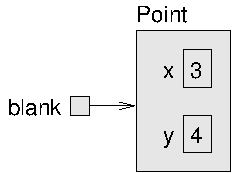
\includegraphics{figs/reference.pdf}
\caption{Memory diagram showing a variable that refers to a \java{Point} object.}
\label{fig.reference}
\end{center}
\end{figure}

As usual, the name of the variable \java{blank} appears outside the box, and its value appears inside the box.
In this case, the value is a reference, which is represented with an arrow.
The arrow points to the new object, which contains two variables, \java{x} and \java{y}.


\section{Attributes}
\label{attribute}

\index{attribute}
\index{dot notation}

Variables that belong to an object are usually called {\bf attributes}, but you might also see them called ``fields''.
To access an attribute of an object, Java uses {\bf dot notation}.
For example:

\begin{code}
int x = blank.x;
\end{code}

The expression \java{blank.x} means ``go to the object \java{blank} refers to, and get the value of the attribute \java{x}.''
In this case, we assign that value to a local variable named \java{x}.
There is no conflict between the local variable named \java{x} and the attribute named \java{x}.
The purpose of dot notation is to identify {\em which} variable you are referring to unambiguously.

You can use dot notation as part of an expression.
For example:

\begin{code}
System.out.println(blank.x + ", " + blank.y);
int sum = blank.x * blank.x + blank.y * blank.y;
\end{code}

The first line displays \java{3, 4}; the second line calculates the value \java{25}.


\section{Objects as parameters}

\index{parameter}
\index{object!as parameter}

You can pass objects as parameters in the usual way.
For example:

\begin{code}
public static void printPoint(Point p) {
    System.out.println("(" + p.x + ", " + p.y + ")");
}
\end{code}

This method takes a point as an argument and displays its attributes in parentheses.
If you invoke \java{printPoint(blank)}, it displays \java{(3, 4)}.

But we don't really need a method like \java{printPoint}, because if you invoke \java{System.out.println(blank)} you get:

\begin{stdout}
java.awt.Point[x=3,y=4]
\end{stdout}

\java{Point} objects provide a method called \java{toString} that returns a string representation of a point.
When you call \java{println} with objects, it automatically calls \java{toString} and displays the result.
In this case, it shows the name of the type (\java{java.awt.Point}) and the names and values of the attributes.

As another example, we can rewrite the \java{distance} method from Section~\ref{distance} so that it takes two \java{Point}s as parameters instead of four \java{double}s.

\begin{code}
public static double distance(Point p1, Point p2) {
    int dx = p2.x - p1.x;
    int dy = p2.y - p1.y;
    return Math.sqrt(dx * dx + dy * dy);
}
\end{code}

Passing objects as parameters makes the source code more readable and less error-prone, because related values are bundled together.


\section{Objects as return types}

\index{Rectangle}
\index{class!Rectangle}

The \java{java.awt} package also provides a class called \java{Rectangle}.
To use it, you have to import it:

\begin{code}
import java.awt.Rectangle;
\end{code}

\java{Rectangle} objects are similar to points, but they have four attributes: \java{x}, \java{y}, \java{width}, and \java{height}.
The following example creates a \java{Rectangle} object and makes the variable \java{box} refer to it:

\begin{code}
Rectangle box = new Rectangle(0, 0, 100, 200);
\end{code}

Figure~\ref{fig.rectangle} shows the effect of this assignment.

\begin{figure}[!ht]
\begin{center}
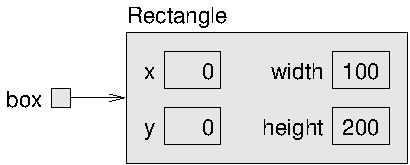
\includegraphics{figs/rectangle.pdf}
\caption{Memory diagram showing a \java{Rectangle} object.}
\label{fig.rectangle}
\end{center}
\end{figure}

If you run \java{System.out.println(box)}, you get:

\begin{stdout}
java.awt.Rectangle[x=0,y=0,width=100,height=200]
\end{stdout}

Again, \java{println} uses the \java{toString} method provided by \java{Rectangle}, which knows how to display \java{Rectangle} objects.

\index{return}
\index{statement!return}

You can write methods that return objects.
For example, \java{findCenter} takes a \java{Rectangle} as an argument and returns a \java{Point} with the coordinates of the center of the rectangle:

\begin{code}
public static Point findCenter(Rectangle box) {
    int x = box.x + box.width / 2;
    int y = box.y + box.height / 2;
    return new Point(x, y);
}
\end{code}

The return type of this method is \java{Point}.
The last line creates a new \java{Point} object and returns a reference to it.


\section{Mutable objects}

\index{mutable}
\index{object!mutable}

You can change the contents of an object by making an assignment to one of its attributes.
For example, to ``move'' a rectangle without changing its size, you can modify the \java{x} and \java{y} values:

\begin{code}
Rectangle box = new Rectangle(0, 0, 100, 200);
box.x = box.x + 50;
box.y = box.y + 100;
\end{code}

The result is shown in Figure~\ref{fig.rectangle2}.

\begin{figure}[!ht]
\begin{center}
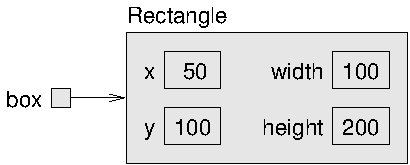
\includegraphics{figs/rectangle2.pdf}
\caption{Memory diagram showing updated attributes.}
\label{fig.rectangle2}
\end{center}
\end{figure}

\index{encapsulation}
\index{generalization}

We can encapsulate this code in a method and generalize it to move the rectangle by any amount:

\begin{code}
public static void moveRect(Rectangle box, int dx, int dy) {
    box.x = box.x + dx;
    box.y = box.y + dy;
}
\end{code}

The variables \java{dx} and \java{dy} indicate how far to move the rectangle in each direction.
Invoking this method has the effect of modifying the \java{Rectangle} that is passed as an argument.

\begin{code}
Rectangle box = new Rectangle(0, 0, 100, 200);
moveRect(box, 50, 100);
System.out.println(box);
\end{code}

%The code displays \java{java.awt.Rectangle[x=50,y=100,width=100,height=200]}.

Modifying objects by passing them as arguments to methods can be useful.
But it can also make debugging more difficult, because it is not always clear which method invocations modify their arguments.

Java provides a number of methods that operate on \java{Point}s and \java{Rectangle}s.
For example, \java{translate} has the same effect as \java{moveRect}, but instead of passing the rectangle as an argument, you use dot notation:

\begin{code}
box.translate(50, 100);
\end{code}

This line invokes the \java{translate} method for the object that \java{box} refers to.
As a result, the \java{box} object is updated directly.

\index{object-oriented}

This example is a good illustration of {\bf object-oriented} programming.
Rather than write methods like \java{moveRect} that modify one or more parameters, we apply methods to objects themselves using dot notation.


\section{Aliasing}
\label{aliasing}

\index{reference}

Remember that when you assign an object to a variable, you are assigning a {\em reference} to an object.
It is possible to have multiple variables that refer to the same object.
The memory diagram in Figure~\ref{fig.aliasing} shows the result.

\begin{code}
Rectangle box1 = new Rectangle(0, 0, 100, 200);
Rectangle box2 = box1;
\end{code}

\begin{figure}[!ht]
\begin{center}
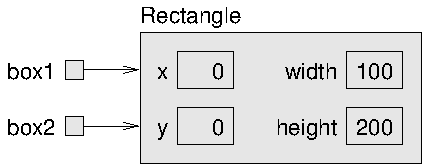
\includegraphics{figs/aliasing.pdf}
\caption{Memory diagram showing two variables that refer to the same object.}
\label{fig.aliasing}
\end{center}
\end{figure}

\index{aliasing}

Notice how \java{box1} and \java{box2} are aliases for the same object, so any changes that affect one variable also affect the other.
This example adds 50 to all four sides of the rectangle, so it moves the corner up and to the left by 50, and it increases the height and width by 100:

\begin{code}
System.out.println(box2.width);
box1.grow(50, 50);
System.out.println(box2.width);
\end{code}

The first line displays {\tt 100}, which is the width of the \java{Rectangle} referred to by \java{box2}.
The second line invokes the \java{grow} method on \java{box1}, which stretches the \java{Rectangle} horizontally and vertically.
The effect is shown in Figure~\ref{fig.aliasing2}.

\begin{figure}[!ht]
\begin{center}
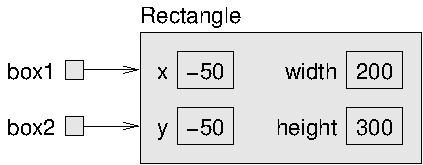
\includegraphics{figs/aliasing2.pdf}
\caption{Memory diagram showing the effect of invoking \java{grow}.}
\label{fig.aliasing2}
\end{center}
\end{figure}

When we make a change using \java{box1}, we see the change using \java{box2}.
Thus, the value displayed by the third line is {\tt 200}, the width of the expanded rectangle.
%(As an aside, it is perfectly legal for the coordinates of a \java{Rectangle} %to be negative.)

%As you can tell from this simple example, code that involves aliasing can get confusing fast, and it can be difficult to debug.
%In general, aliasing should be avoided or used with care.


\section{The null keyword}

\index{null}

When you create an object variable, remember that you are storing a reference to an object.
In Java, the keyword \java{null} is a special value that means ``no object''.
You can declare and initialize object variables this way:

\begin{code}
Point blank = null;
\end{code}

The value \java{null} is represented in memory diagrams by a small box with no arrow, as in Figure~\ref{fig.reference2}.

\begin{figure}[!ht]
\begin{center}

\includegraphics{figs/reference2.pdf}
\caption{Memory diagram showing a variable that contains a \java{null} reference.}
\label{fig.reference2}
\end{center}
\end{figure}

\index{exception!NullPointer}
\index{NullPointerException}
\index{run-time error}

If you try to use a \java{null} value, either by accessing an attribute or invoking a method, Java throws a \java{NullPointerException}.

\begin{code}
Point blank = null;
int x = blank.x;              // NullPointerException
blank.translate(50, 50);      // NullPointerException
\end{code}

On the other hand, it is legal to pass a null reference as an argument or receive one as a return value.
For example, \java{null} is often used to represent a special condition or indicate an error.


\section{Garbage collection}

In Section~\ref{aliasing}, we saw what happens when more than one variable refers to the same object.
What happens when {\em no} variables refer to an object?

\begin{code}
Point blank = new Point(3, 4);
blank = null;
\end{code}

The first line creates a new \java{Point} object and makes \java{blank} refer to it.
The second line changes \java{blank} so that instead of referring to the object, it refers to nothing.
In the memory diagram, we remove the arrow between them, as in Figure~\ref{fig.reference3}.

\begin{figure}[!ht]
\begin{center}
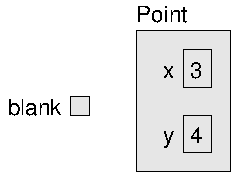
\includegraphics{figs/reference3.pdf}
\caption{Memory diagram showing the effect of setting a variable to \java{null}.}
\label{fig.reference3}
\end{center}
\end{figure}

If there are no references to an object, there is no way to access its attributes or invoke a method on it.
From the programmer's view, it ceases to exist.
However it's still present in the computer's memory, taking up space.

\index{garbage collection}

As your program runs, the system automatically looks for stranded objects and reclaims them; then the space can be reused for new objects.
This process is called {\bf garbage collection}.

You don't have to do anything to make garbage collection happen, and in general don't have to be aware of it.
But in high-performance applications, you may notice a slight delay every now and then when Java reclaims space from discarded objects.
%You can manually run the garbage collector by invoking \java{System.gc()} method.


\section{Class diagrams}
\label{UML}

To summarize what we've learned so far, \java{Point} and \java{Rectangle} objects each have their own attributes and methods.
Attributes are an object's {\em data}, and methods are an object's {\em code}.
An object's class defines which attributes and methods it will have.

\index{UML}

In practice, it's more convenient to look at high-level pictures than to examine the source code.
{\bf Unified Modeling Language} (UML) defines a standard way to summarize the design of a class.

\begin{figure}[!ht]
\begin{center}
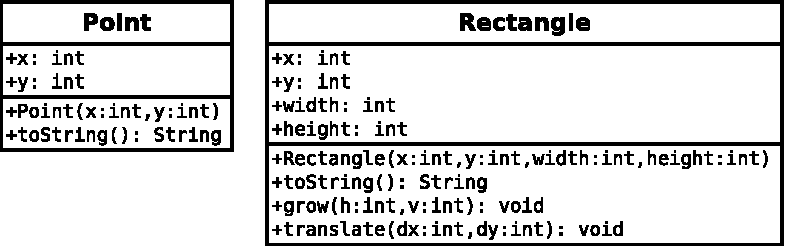
\includegraphics{figs/point-rect.pdf}
\caption{UML class diagrams for \java{Point} and \java{Rectangle}.}
\label{fig.umlPoint}
\end{center}
\end{figure}

\index{class diagram}
\index{diagram!class}

As shown in Figure~\ref{fig.umlPoint}, a {\bf class diagram} is divided into two sections.
The top half lists the attributes, and the bottom half lists the methods.
UML uses a language-independent format, so rather than showing \java{int x}, the diagram uses {\tt x:~int}.

In contrast to memory diagrams, which visualize objects (and variables) at run-time, a class diagram visualizes the source code at compile-time.

Both \java{Point} and \java{Rectangle} have additional methods; we are only showing the ones introduced in this chapter.
See the documentation for these classes to learn more about what they can do.


\section{Java library source}
\label{src.zip}

\index{library}
\index{source code}

Throughout the book, you have used classes from the Java library including \java{System}, \java{String}, \java{Scanner}, \java{Math}, \java{Random}, and others.
You may not have realized that these classes are written in Java.
In fact, you can take a look at the source code to see how they work.

\index{src.zip}

The Java library contains thousands of files, many of which are thousands of lines of code.
That's more than one person could read and understand fully, so please don't be intimidated!

Because it's so large, the library source code is stored in a file named \java{src.zip}.
Take a few minutes to locate this file on your machine:

\begin{itemize}
\item On Linux, it's likely under: \verb"/usr/lib/jvm/openjdk-8/"
\\ (You might need to install the {\tt openjdk-8-source} package.)
\item On OS X, it's likely under: \\ \verb"/Library/Java/JavaVirtualMachines/jdk.../Contents/Home/"
\item On Windows, it's likely under: \verb"C:\Program Files\Java\jdk...\"
\end{itemize}

When you open (or unzip) the file, you will see folders that correspond to Java packages.
For example, open the {\tt java} folder and then open the {\tt awt} folder.
You should now see {\tt Point.java} and {\tt Rectangle.java}, along with the other classes in the \java{java.awt} package.

Open {\tt Point.java} in your editor and skim through the file.
It uses language features we haven't yet discussed, so you probably won't understand everything.
But you can get a sense of what professional Java software looks like by browsing through the library.

\index{documentation}
\index{HTML}
\index{Javadoc}

Notice how much of {\tt Point.java} is documentation (see Appendix~\ref{app:javadoc}).
Each method is thoroughly commented, including \java{@param}, \java{@return}, and other tags.
Javadoc reads these comments and generates documentation in HTML.
You can see the results by reading the documentation for the \java{Point} class, which you can find by doing a web search for ``Java Point''.

Now take a look at \java{Rectangle}'s \java{grow} and \java{translate} methods.
There is more to them than you may have realized, but that doesn't limit your ability to use these methods in a program.

To summarize the whole chapter, objects encapsulate data and provide methods to access and modify the data directly.
Object-oriented programming makes it possible to hide messy details so that you can more easily use and understand code that other people wrote.


\section{Vocabulary}

\begin{description}

\term{attribute}
One of the named data items that make up an object.
%Each object has its own copy of the attributes for its class.

\term{dot notation}
Use of the dot operator (\java{.}) to access an object's attributes or methods.

\term{object-oriented}
A way of organizing code and data into objects, rather than independent methods.

\term{garbage collection}
The process of finding objects that have no references and reclaiming their storage space.

\term{UML}
Unified Modeling Language, a standard way to draw diagrams for software engineering.

\term{class diagram}
An illustration of the attributes and methods for a class.

\end{description}


\section{Exercises}

The code for this chapter is in the {\tt ch10} directory of {\tt ThinkJava2Code}.
See page~\pageref{code} for instructions on how to download the repository.
Before you start the exercises, we recommend that you compile and run the examples.

At this point you know enough to read Appendix~\ref{graphics}, which is about simple 2D graphics and animations.
During the next few chapters, you should take a detour to read this appendix and work through the exercises.


\begin{exercise}  %%V6 Ex10.1

The point of this exercise is to make sure you understand the mechanism for passing objects as parameters.

\begin{enumerate}

\item For the following program, draw a stack diagram showing the local variables and parameters of \java{main} and \java{riddle} just before \java{riddle} returns.
Use arrows to show which objects each variable references.

\item What is the output of the program?

\item Is the \java{blank} object mutable or immutable?
How can you tell?

\end{enumerate}

\begin{code}
public static int riddle(int x, Point p) {
    x = x + 7;
    return x + p.x + p.y;
}
\end{code}

\begin{code}
public static void main(String[] args) {
    int x = 5;
    Point blank = new Point(1, 2);

    System.out.println(riddle(x, blank));
    System.out.println(x);
    System.out.println(blank.x);
    System.out.println(blank.y);
}
\end{code}

\end{exercise}


\begin{exercise}  %%V6 Ex10.2

The point of this exercise is to make sure you understand the mechanism for returning new objects from methods.

\begin{enumerate}

\item Draw a stack diagram showing the state of the program just before \java{distance} returns.
Include all variables and parameters, and show the objects those variables refer to.

\item What is the output of this program?
(Can you tell without running it?)

\end{enumerate}

\begin{code}
public static double distance(Point p1, Point p2) {
    int dx = p2.x - p1.x;
    int dy = p2.y - p1.y;
    return Math.sqrt(dx * dx + dy * dy);
}

public static Point findCenter(Rectangle box) {
    int x = box.x + box.width / 2;
    int y = box.y + box.height / 2;
    return new Point(x, y);
}
\end{code}

\begin{code}
public static void main(String[] args) {
    Point blank = new Point(5, 8);

    Rectangle rect = new Rectangle(0, 2, 4, 4);
    Point center = findCenter(rect);

    double dist = distance(center, blank);
    System.out.println(dist);
}
\end{code}

\end{exercise}


\begin{exercise}  %%V6 Ex10.3

This exercise is about aliasing.
Recall that aliases are two variables that refer to the same object.

\begin{enumerate}

\item Draw a diagram that shows the state of the program just before the end of \java{main}.
Include all local variables and the objects they refer to.

\item What is the output of the program?

\item At the end of \java{main}, are \java{p1} and \java{p2} aliased?
Why or why not?

\end{enumerate}

\begin{code}
public static void printPoint(Point p) {
    System.out.println("(" + p.x + ", " + p.y + ")");
}

public static Point findCenter(Rectangle box) {
    int x = box.x + box.width / 2;
    int y = box.y + box.height / 2;
    return new Point(x, y);
}
\end{code}

\begin{code}
public static void main(String[] args) {
    Rectangle box1 = new Rectangle(2, 4, 7, 9);
    Point p1 = findCenter(box1);
    printPoint(p1);

    box1.grow(1, 1);
    Point p2 = findCenter(box1);
    printPoint(p2);
}
\end{code}

\end{exercise}


\begin{exercise}  %%V6 Ex10.4
\label{ex.biginteger}

\index{factorial}

You might be sick of the factorial method by now, but we're going to do one more version.

\begin{enumerate}

\item Create a new program called {\tt Big.java} and write (or reuse) an iterative version of \java{factorial}.

\item Display a table of the integers from 0 to 30 along with their factorials.
At some point around 15, you will probably see that the answers are not right anymore.
Why not?

\index{BigInteger}

\item \java{BigInteger} is a Java class that can represent arbitrarily big integers.
There is no upper bound except the limitations of memory size and processing speed.
Take a minute to read the documentation, which you can find by doing a web search for ``Java BigInteger''.

\item To use BigIntegers, you have to import \java{java.math.BigInteger} at the beginning of your program.

\item There are several ways to create a BigInteger, but the simplest uses \java{valueOf}.
The following code converts an integer to a BigInteger:

\begin{code}
int x = 17;
BigInteger big = BigInteger.valueOf(x);
\end{code}

%Type in this code and try it out.
%Try displaying a BigInteger.

\item Since BigIntegers are not primitive types, the usual math operators don't work.
Instead, we have to use methods like \java{add}.
To add two BigIntegers, invoke \java{add} on one and pass the other as an argument.

\begin{code}
BigInteger small = BigInteger.valueOf(17);
BigInteger big = BigInteger.valueOf(1700000000);
BigInteger total = small.add(big);
\end{code}

Try out some of the other methods, like \java{multiply} and \java{pow}.

\item Convert \java{factorial} so that it performs its calculation using BigIntegers and returns a BigInteger as a result.
You can leave the parameter alone; it will still be an integer.

\item Try displaying the table again with your modified factorial method.
Is it correct up to 30?
How high can you make it go?

\item Are BigInteger objects mutable or immutable?
How can you tell?

\end{enumerate}

\end{exercise}


\begin{exercise}  %%V6 Ex10.5

Many encryption algorithms depend on the ability to raise large integers to a power.
Here is a method that implements an efficient algorithm for integer exponentiation:

\begin{code}
public static int pow(int x, int n) {
    if (n == 0) return 1;

    // find x to the n/2 recursively
    int t = pow(x, n / 2);

    // if n is even, the result is t squared
    // if n is odd, the result is t squared times x
    if (n % 2 == 0) {
        return t * t;
    } else {
        return t * t * x;
    }
}
\end{code}

\index{BigInteger}

The problem with this method is that it only works if the result is small enough to be represented by an \java{int}.
Rewrite it so that the result is a \java{BigInteger}.
The parameters should still be integers, though.

You should use the \java{BigInteger} methods \java{add} and \java{multiply}.
But don't use \java{BigInteger.pow}; that would spoil the fun.

\end{exercise}


\chapter{Designing Classes}

\index{object!type}
\index{type!object}

Whenever you create a new class, you are creating a new object type with the same name.
So way back in Section~\ref{hello}, when we created the class \java{Hello}, we also created an object type named \java{Hello}.

We didn't declare any variables with type \java{Hello}, and we didn't use \java{new} to create \java{Hello} objects.
And it wouldn't have done much good if we had -- but we could have!

In this chapter, you will learn to design classes that represent {\em useful} objects.  Here are the main ideas:

\begin{itemize}

\item Again, defining a {\bf class} creates a new object type with the same name.

\index{class!definition}

\item A {\bf class} definition is a template for objects: it specifies what attributes the objects have and what methods can operate on them.

\index{instance}

\item Every object belongs to some object type; that is, it is an {\bf instance} of some class.

\index{instantiate}

\item The \java{new} operator {\bf instantiates} objects; that is, it creates new instances of a class.

%\item The design of a class (what methods it has) determines whether the objects are mutable or immutable.

\item The methods that operate on an object type are defined in the class for that object.

\end{itemize}

Think of a class like a blueprint for a house: you can use the same blueprint to build any number of houses.

\section{The Time Class}

\index{data encapsulation}
\index{encapsulation!data}

A common reason to define a new class is to encapsulate related data in an object that can be treated as a single unit.
That way, we can use objects as parameters and return values, rather than passing and returning multiple values.
%This design principle is called {\bf data encapsulation}.
We have already seen two types that encapsulate data in this way: \java{Point} and \java{Rectangle}.

\index{class!Time}
\index{Time}

Another example, which we will implement ourselves, is \java{Time}, which represents a time of day.
The data encapsulated in a \java{Time} object include an hour, a minute, and a number of seconds.
Because every \java{Time} object contains these values, we define attributes to hold them.

\index{instance variable}
\index{variable!instance}

Attributes are also called {\bf instance variables}, because each instance has its own variables (as opposed to ``class variables'', coming up in Section~\ref{classvar}).

The first step is to decide what type each variable should be.
It seems clear that \java{hour} and \java{minute} should be integers.
Just to keep things interesting, let's make \java{second} a double.

Instance variables are declared at the beginning of the class definition, outside of any method.
By itself, this code fragment is a legal class definition:

\begin{code}
public class Time {
    private int hour;
    private int minute;
    private double second;
}
\end{code}

\index{private}
\index{variable!private}

The \java{Time} class is \java{public}, which means that it can be used in other classes.
But the instance variables are \java{private}, which means they can only be accessed from inside the \java{Time} class.
If you try to read or write them from another class, you will get a compiler error.

\index{information hiding}

Private instance variables help keep classes isolated from each other, so that changes in one class won't require changes in other classes.
It also simplifies what other programmers need to know to use your classes.
This kind of isolation is called {\bf information hiding}.


\section{Constructors}

\index{constructor}
\index{method!constructor}

After declaring instance variables, the next step is to define a {\bf constructor}, which is a special method that initializes the object.
The syntax for constructors is similar to that of other methods, except:

\index{static}

\begin{itemize}

\item The name of the constructor is the same as the name of the class.

\item Constructors have no return type (and no return value).

\item The keyword \java{static} is omitted.

\end{itemize}

Here is an example constructor for the \java{Time} class:

\begin{code}
public Time() {
    this.hour = 0;
    this.minute = 0;
    this.second = 0.0;
}
\end{code}

This constructor does not take any arguments.
Each line initializes an instance variable to zero (which is ``midnight'' for a \java{Time} object).

\index{this}
\index{keyword}

The name \java{this} is a keyword that refers to the object we are creating.
You can use \java{this} the same way you use the name of any other object.
For example, you can read and write the instance variables of \java{this}, and you can pass \java{this} as an argument to other methods.
But you do not declare \java{this}, and you can't make an assignment to it.

A common error when writing constructors is to put a \java{return} statement at the end.
Like \java{void} methods, constructors do not return values.

To create a \java{Time} object, you must use the \java{new} operator:

\begin{code}
public static void main(String[] args) {
    Time time = new Time();
}
\end{code}

\index{new}
\index{operator!new}

When you use \java{new}, Java creates the object and invokes your constructor to initialize the instance variables.
When the constructor is done, \java{new} returns a reference to the new object.
In this example, the reference gets assigned to the variable \java{time}, which has type \java{Time}.
Figure~\ref{fig.time} shows the result.

\index{memory diagram}
\index{diagram!memory}

\begin{figure}[!ht]
\begin{center}
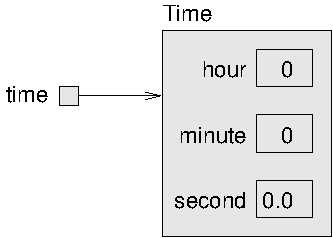
\includegraphics{figs/time.pdf}
\caption{Memory diagram of a \java{Time} object.}
\label{fig.time}
\end{center}
\end{figure}

\index{recursion!infinite}
\index{infinite recursion}
\index{StackOverflowError}

Beginners sometimes make the mistake of using \java{new} in the constructor:

\begin{code}
public Time() {
    new Time();         // StackOverflowError
    this.hour = 0;
    this.minute = 0;
    this.second = 0.0;
}
\end{code}

Doing so causes an infinite recursion, since \java{new} invokes the {\em same} constructor, which uses \java{new} again, which invokes the constructor again, and so on.

%If you don't provide a constructor for a class, Java will generate one for you automatically.
%The default constructor takes no arguments and initializes all attributes to zero (or an equivalent value like \java{false} or \java{null}).


\section{More Constructors}

\index{overload}

Like other methods, constructors can be overloaded, which means you can provide multiple constructors with different parameters.
Java knows which constructor to invoke by matching the arguments you provide with the parameters of the constructor.

\index{value constructor}
\index{constructor!value}

It is common to provide both a ``default constructor'' that takes no arguments, like the previous one, and a ``value constructor'', like this one:

\begin{code}
public Time(int hour, int minute, double second) {
    this.hour = hour;
    this.minute = minute;
    this.second = second;
}
\end{code}

\index{shadow}

All this constructor does is copy values from the parameters to the instance variables.
%In this example, the names and types of the parameters are the same as the instance variables.
Notice that the parameters shadow (or hide) the instance variables, so the keyword \java{this} is necessary to tell them apart.
Parameters don't have to use the same names, but that's a common style.

%TODO Let's make sure the discussion of shadowing comes before this.

To invoke this second constructor, you have to provide arguments to the \java{new} operator.
The following example creates a \java{Time} object that represents a fraction of a second before noon:

\begin{code}
Time time = new Time(11, 59, 59.9);
\end{code}

Here is the complete class definition so far:

%\index{Time.java}

\begin{code}%{Time.java}
public class Time {
    private int hour;
    private int minute;
    private double second;

    public Time() {
        this.hour = 0;
        this.minute = 0;
        this.second = 0.0;
    }

    public Time(int hour, int minute, double second) {
        this.hour = hour;
        this.minute = minute;
        this.second = second;
    }
}
\end{code}

Overloading constructors provides the flexibility to create an object first and then fill in the attributes, or collect all the information before creating the object itself.

Once you get the hang of it, writing constructors gets boring.
You can write them quickly just by looking at the list of instance variables.
In fact, some IDEs can generate them for you.


\section{Getters and Setters}

Recall that the instance variables of \java{Time} are \java{private}.
We can access them from within the \java{Time} class, but if we try to read or write them from another class, the compiler reports an error.

\index{private}
\index{variable!private}

A class that uses objects defined in another class is called a {\bf client}.
For example, here is a new class called \java{TimeClient}.

\index{client}

\begin{code}
public class TimeClient {

    public static void main(String[] args) {
        Time time = new Time(11, 59, 59.9);
        System.out.println(time.hour);      // compiler error
    }
}
\end{code}

If you compile this code, you get an error message like ``hour has private access in Time''.
There are three ways to solve this problem:

\begin{itemize}

\item We could make the instance variables public.

\item We could provide methods to access the instance variables.

\item We could decide that it's not a problem, and refuse to let other classes access the instance variables.

\end{itemize}

The first choice is appealing because it's simple.
But here is the problem: when Class $A$ accesses the instance variables of Class $B$ directly, $A$ becomes dependent on $B$.
If anything in $B$ changes later, it is likely that $A$ will have to change, too.

\index{dependent}
\index{independent}

But if $A$ only uses methods to interact with $B$, $A$ and $B$ are less dependent, which means that we can make changes in $B$ without affecting $A$ (as long as we don't change the method parameters).
So we generally avoid making instance variables public.

The second option is to provide methods that access the instance variables.
For example, we might want the instance variables to be ``read only''; that is, code in other classes should be able to read them but not write them.
We can do that by providing one method for each instance variable:

\begin{code}
public int getHour() {
    return this.hour;
}

public int getMinute() {
    return this.minute;
}

public double getSecond() {
    return this.second;
}
\end{code}

\index{accessor}
\index{method!accessor}
\index{getter}
\index{method!getter}

Methods like these are formally called ``accessors'', but more commonly referred to as {\bf getters}.
By convention, the method that gets a variable named \java{something} is called \java{getSomething}.

We can fix the compiler error in \java{TimeClient} by using the getter:

\begin{code}
System.out.println(time.getHour());
\end{code}

If we decide that \java{TimeClient} should also be able to modify the instance variables of \java{Time}, we can provide methods to do that, too:

\begin{code}
public void setHour(int hour) {
    this.hour = hour;
}

public void setMinute(int minute) {
    this.minute = minute;
}

public void setSecond(double second) {
    this.second = second;
}
\end{code}

\index{mutator}
\index{method!mutator}
\index{setter}
\index{method!setter}

These methods are formally called ``mutators'', but more commonly known as {\bf setters}.
The naming convention is similar; the method that sets \java{something} is usually called \java{setSomething}.

Writing getters and setters can get boring, but many IDEs can generate them for you based on the instance variables.

% NOTE: A thougtful reader might ask a question we don't answer here: if we provide getters and setters, why don't we just make the instance variables public? 


\section{Displaying Objects}

To display \java{Time} objects we can write a method to display the hour, minute, and second.
Using \java{printTime} in Section~\ref{multparam} as a starting point, we could write:

\begin{code}
public static void printTime(Time t) {
    System.out.print(t.hour);
    System.out.print(":");
    System.out.print(t.minute);
    System.out.print(":");
    System.out.println(t.second);
}
\end{code}

The output of this method, given the \java{time} object from the first example, would be {\tt 11:59:59.9}.
We can use \java{printf} to make the code more concise:

\index{printf}
\index{print statement}
\index{format string}

\begin{code}
public static void printTime(Time t) {
    System.out.printf("%02d:%02d:%04.1f\n",
        t.hour, t.minute, t.second);
}
\end{code}

As a reminder, you need to use \java{\%d} with integers and \java{\%f} with floating-point numbers.
The \java{02} option means ``total width 2, with leading zeros if necessary'', and the \java{04.1} option means ``total width 4, one digit after the decimal point, leading zeros if necessary''.
The output is the same: {\tt 11:59:59.9}.

There's nothing wrong with a method like \java{printTime}, but it is not consistent with object-oriented style.
A more idiomatic solution is to provide a special method called \java{toString}.


\section{The toString Method}

Every object has a method called \java{toString} that returns a string representation of the object.
When you display an object using \java{print} or \java{println}, Java invokes the object's \java{toString} method.

\index{override}

By default it simply displays the type of the object and its address in hexadecimal. 
So, if you create a \java{Time} object and display it with \java{println}:

\begin{code}
public static void main(String[] args) {
    Time time = new Time(11, 59, 59.9);
    System.out.println(time);
}
\end{code}

\index{print}
\index{statement!print}
\index{object!displaying}

The output looks something like this:

\begin{stdout}
Time@80cc7c0
\end{stdout}

\index{address}
\index{hexadecimal}

This address can be useful for debugging, if you want to keep track of individual objects.

\index{toString}
\index{method!toString}

But you can {\bf override} this behavior by providing your own \java{toString} method.
For example, here is a \java{toString} method for \java{Time}:

\begin{code}
public String toString() {
    return String.format("%02d:%02d:%04.1f\n",
        this.hour, this.minute, this.second);
}
\end{code}

\index{instance method}
\index{method!instance}

The definition does not have the keyword \java{static}, because it is not a static method.
It is an {\bf instance method}, so called because when you invoke it, you invoke it on an instance of the class.
Instance methods are sometimes called ``non-static''; you might see this term in an error message.

The body of the method is similar to \java{printTime} in the previous section, with two changes:

\begin{itemize}

\item Inside the method, we use \java{this} to refer to the current instance; that is, the object the method is invoked on.

\item Instead of \java{printf}, it uses \java{String.format}, which returns a formatted \java{String} rather than displaying it.

\end{itemize}

\index{string!format}

Now you can call \java{toString} directly:

\begin{code}
Time time = new Time(11, 59, 59.9);
String s = time.toString();
\end{code}

The value of \java{s} is the \java{String} \java{"11:59:59.9"}.

You can also invoke \java{toString} indirectly by invoking \java{print} or \java{println}:

\begin{code}
System.out.println(time);
\end{code}

This code displays the \java{String} \java{"11:59:59.9"}. 

Either way, when you use \java{this} inside \java{toString}, it refers to the same object as \java{time}.


\section{The equals Method}
\label{equals}

\index{== equals operator}
\index{equals}
\index{method!equals}

We have seen two ways to check whether values are equal: the \java{==} operator and the \java{equals} method.
With objects you can use either one, but they are not the same.

\begin{itemize}

\index{identical}

\item The \java{==} operator checks whether two references are {\bf identical}; that is, whether they refer to the same object.

\index{equivalent}

\item The \java{equals} method checks whether two objects are {\bf equivalent}; that is, whether they have the same values.

\end{itemize}

The definition of identity is always the same, so the \java{==} operator always does the same thing.
But the definition of equivalence is different for different objects, so objects can define their own \java{equals} methods.

Consider the following variables and the memory diagram in Figure~\ref{fig.time2}.

\begin{code}
Time time1 = new Time(9, 30, 0.0);
Time time2 = time1;
Time time3 = new Time(9, 30, 0.0);
\end{code}

\index{memory diagram}
\index{diagram!memory}

\begin{figure}[!ht]
\begin{center}
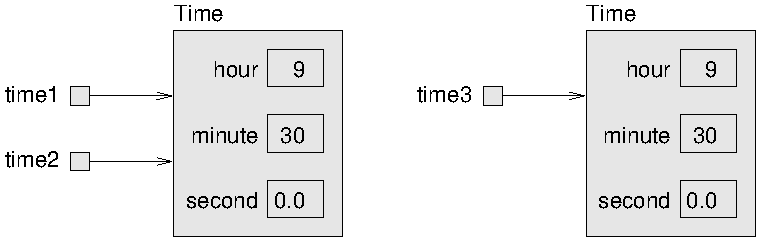
\includegraphics{figs/time2.pdf}
\caption{Memory diagram of three \java{Time} variables.}
\label{fig.time2}
\end{center}
\end{figure}

The assignment operator copies references, so \java{time1} and \java{time2} refer to the same object.
Because they are identical, \java{time1 == time2} is true.
But \java{time1} and \java{time3} refer to two different objects.
Because they are not identical, \java{time1 == time3} is false.

By default, the \java{equals} method does the same thing as \java{==}.
For \java{Time} objects, that's probably not what we want.
For example, \java{time1} and \java{time3} represent the same time of day, so we should consider them equivalent.

\index{equals}
\index{method!equals}

We can provide an \java{equals} method that implements this idea:

\begin{code}
public boolean equals(Time that) {
    final EPS = 0.001;
    return this.hour == that.hour
        && this.minute == that.minute
        && Math.abs(this.second - that.second) < EPS;
}
\end{code}

\java{equals} is an instance method, so it doesn't have the keyword \java{static}.
It uses \java{this} to refer to current object, and \java{that} to refer to the other.
\java{that} is {\em not} a keyword, so we could have given this parameter a different name.
But using \java{that} makes the code nicely readable. 

We can invoke \java{equals} like this:

\begin{code}
time1.equals(time3);
\end{code}

Inside the \java{equals} method, \java{this} refers to the same object as \java{time1}, and \java{that} refers to the same object as \java{time3}.
Since their instance variables are ``equal'', the result is \java{true}.

Because \java{hour} and \java{minute} are integers, we compare them with \java{==}.  
But \java{second} is a floating-point number.  
Because of rounding errors, it is not good to compare floating-point numbers with \java{==} (see Section~\ref{rounderr}).
Instead, we check whether the difference is smaller than a threshold, \java{EPS}.

Many objects have a similar notion of equivalence; that is, two objects are considered equal if their instance variables are equal.
But other definitions are possible.


% This example is a little non-idiomatic.  Can we think of something else?

%You could, for example, allow a \java{Time} object and a \java{String} object to be considered equal if they represent the same time.
%
%\begin{code}
%public boolean equals(String str) {
%    return str.equals(this.toString());
%}
%\end{code}
%
%The \java{equals} method is now overloaded.
%If we invoke \java{time1.equals(time3)}, the first method will be used; \java{time1.equals("09:30:00.0")} uses the second.


\section{Adding Times}

Suppose you are going to a movie that starts at 18:50 (that is, 6:50 PM), and the running time is 2 hours 16 minutes.
What time does the movie end?
We'll use \java{Time} objects to figure it out.

\begin{code}
Time startTime = new Time(18, 50, 0.0);
Time runningTime = new Time(2, 16, 0.0);
\end{code}

\index{Time!addition}
\index{addition!time}

Here are two ways we could ``add'' the \java{Time} objects:

\begin{itemize}

\item We could write a static method that takes two \java{Time} objects as parameters.

\item We could write an instance method that gets invoked on one object and takes the other as a parameter.

\end{itemize}

To demonstrate the difference, we'll do both.
Here is the static method:

\index{static}
\index{method!static}

\begin{code}
public static Time add(Time t1, Time t2) {
    Time sum = new Time();
    sum.hour = t1.hour + t2.hour;
    sum.minute = t1.minute + t2.minute;
    sum.second = t1.second + t2.second;
    return sum;
}
\end{code}

And here's how we would invoke it:

\begin{code}
Time endTime = Time.add(startTime, runningTime);
\end{code}

Here's what it looks like as an instance method:

\index{instance method}
\index{method!instance}

\begin{code}
public Time add(Time t2) {
    Time sum = new Time();
    sum.hour = this.hour + t2.hour;
    sum.minute = this.minute + t2.minute;
    sum.second = this.second + t2.second;
    return sum;
}
\end{code}

And here's how we would invoke it:

\begin{code}
Time endTime = startTime.add(runningTime);
\end{code}

Notice the differences:

\begin{itemize}

\item The static method has the keyword \java{static}; the instance method does not.

\item The static method has two parameters, \java{t1} and \java{t2}.
The instance method has one explicit parameter, \java{t1}, and the implicit parameter, \java{this}.

\item We invoked the static method with the \java{Time} class;
we invoked the instance method with the \java{startTime} object.

\end{itemize}

%Optionally, you could replace \java{t2} with \java{that}.
%Unlike \java{this}, \java{that} is not a keyword; it's just a slightly clever variable name.

That's all there is to it.
Static methods and instance methods do the same thing, and you can convert from one to the other with just a few changes.

However, there's a problem with both of these methods; they are not correct.
The result from either method is {\tt 20:66}, which is not a valid time.

If \java{second} exceeds 59, we have to ``carry'' into the minutes column, and if \java{minute} exceeds 59, we have to carry into \java{hour}.

Here is a better version of the instance method, \java{add}:

\begin{code}
public Time add(Time t2) {
    Time sum = new Time();
    sum.hour = this.hour + t2.hour;
    sum.minute = this.minute + t2.minute;
    sum.second = this.second + t2.second;
    
    if (sum.second >= 60.0) {
        sum.second -= 60.0;
        sum.minute += 1;
    }
    if (sum.minute >= 60) {
        sum.minute -= 60;
        sum.hour += 1;
    }
    return sum;
}
\end{code}

It's still possible that \java{hour} may exceed 23, but there's no \java{days} attribute to carry into.
In that case, \java{sum.hour -= 24} would yield the correct result.


\section{Modifier Methods}

In the previous section, the \java{add} method did not modify the parameters \java{t1} or \java{t2}.
Instead, it created and returned a new \java{Time} object.

Alternatively, we could have written a method like this:

\begin{code}
public void increment(double seconds) {
    this.second += seconds;

    // carry extra seconds
    this.minute += this.second / 60;
    this.second = this.second % 60;

    // carry extra minutes
    this.hour += this.minute / 60;
    this.minute = this.minute % 60;
}
\end{code}

The \java{increment} method modifies an existing \java{Time} object.
It doesn't create a new one, and it doesn't return anything.

\index{modifier method}
\index{method!modifier}

Methods like \java{increment} are called {\bf modifier} methods.
They are usually void, but sometimes they return a reference to the object they modify.

\index{pure method}
\index{method!pure}

In contrast, methods like \java{add} are called {\bf pure} methods, because:

\begin{itemize}

\item They don't modify the parameters.

\item They don't have any other ``side effects'', like printing.

\item The return value only depends on the parameters, not on any other data.

\end{itemize}

Modifiers can be more efficient because they don't create new objects.
But they can also be error-prone.
Especially when objects are aliased, the effects of modifiers can be confusing.

%\index{immutable}

%If a class provides only getters and pure methods (no setters or modifiers), then the objects will be immutable.
%Working with immutable objects can be more difficult at first, but they can save you from long hours of debugging.


\section{Vocabulary}

\begin{description}

\term{class}
Previously, we defined a class as a collection of related methods.
Now you know that a class is also a template for a new type of object.

\term{instance}
A member of a class.
Every object is an instance of some class.

\term{instantiate}
Create a new instance of a class in the computer's memory.

%\term{data encapsulation}
%A technique for bundling multiple named variables into a single object.

\term{instance variable}
An attribute of an object; a non-static variable defined at the class level.

\term{information hiding}
The practice of making instance variables \java{private} to limit dependencies between classes.

\term{constructor}
A special method that initializes the instance variables of a newly-constructed object.

%\term{shadow}
%Defining a local variable or parameter with the same name and type as an instance variable.

\term{client}
A class that uses objects defined in another class.

\term{getter}
A method that returns the value of an instance variable.

\term{setter}
A method that assigns a value to an instance variable.

\term{override}
Replacing a default implementation of a method, such as \java{toString}.

\term{instance method}
A non-static method that has access to \java{this} and the instance variables.

\term{identical}
References to the same object or the same location in memory are identical.

\term{equivalent}
Two objects that are ``equal'' but not necessarily identical, as defined by the \java{equals} method.

\term{modifier method}
A method that changes the state (instance variables) of an object.

\term{pure method}
A method that depends only on its parameters (including the implicit parameter \java{this}) and no other data.

\end{description}


\section{Exercises}

The code for this chapter is in the {\tt ch11} directory of {\tt ThinkJavaCode2}.
See page~\pageref{code} for instructions on how to download the repository.
Before you start the exercises, we recommend that you compile and run the examples.


\begin{exercise}  %%V6 Ex11.1

Review the documentation of \java{java.awt.Rectangle}.
Which methods are pure?
Which are modifiers?

If you review the documentation of \java{java.lang.String}, you should see that there are no modifiers, because strings are immutable.

\end{exercise}


\begin{exercise}  %%V6 Ex11.2

The implementation of \java{increment} in this chapter is not very efficient.
Can you rewrite it so it doesn't use any loops?

{\it Hint:} Remember the remainder operator. And yes, it works with floating-point values too.

\end{exercise}


\begin{exercise}  %%V6 Ex11.3
\index{Scrabble}

In the board game Scrabble, each tile contains a letter, which is used to spell words in rows and columns, and a score, which is used to determine the value of words.

\begin{enumerate}

\item Write a definition for a class named \java{Tile} that represents Scrabble tiles.
The instance variables should include a character named \java{letter} and an integer named \java{value}.

\item Write a constructor that takes parameters named \java{letter} and \java{value} and initializes the instance variables.

\item Write a method named \java{printTile} that takes a \java{Tile} object as a parameter and displays the instance variables in a reader-friendly format.

\item Write a \java{main} method that creates a \java{Tile} object with the letter \java{Z} and the value \java{10}, and then uses \java{printTile} to display the state of the object.

\item Implement the \java{toString} and \java{equals} methods for a \java{Tile}.

\item Create getters and setters for each of the attributes.

\end{enumerate}

The point of this exercise is to practice the mechanical part of creating a new class definition.
\end{exercise}


\begin{exercise}  %%V6 Ex11.4

Write a class definition for \java{Date}, an object type that contains three integers: \java{year}, \java{month}, and \java{day}.
This class should provide two constructors.
The first should take no parameters and initialize a default date.
The second should take parameters named \java{year}, \java{month} and \java{day}, and use them to initialize the instance variables.

Write a \java{main} method that creates a new \java{Date} object named \java{birthday}.
The new object should contain your birth date.
You can use either constructor.
%Compare your implementation to \java{java.util.Date}.

\end{exercise}


\begin{exercise}  %%V6 Ex11.5

\index{rational number}

A rational number is a number that can be represented as the ratio of two integers.
For example, $2/3$ is a rational number, and you can think of 7 as a rational number with an implicit 1 in the denominator.
%The goal of this exercise is to write a class definition for rational numbers.

\begin{enumerate}

\item Define a class called \java{Rational}.
A \java{Rational} object should have two integer instance variables that store the numerator and denominator.

\item Write a constructor that takes no arguments and that sets the numerator to 0 and denominator to 1.

\item Write an instance method called \java{printRational} that displays a \java{Rational} in some reasonable format.

\item Write a \java{main} method that creates a new object with type \java{Rational}, sets its instance variables to the values of your choice, and displays the object.

\item At this stage, you have a minimal testable program.
Test it and, if necessary, debug it.

\item Write a \java{toString} method for \java{Rational} and test it using \java{println}.

\item Write a second constructor that takes two arguments and uses them to initialize the instance variables.

\item Write an instance method called \java{negate} that reverses the sign of a rational number.
This method should be a modifier, so it should be void.
Add lines to \java{main} to test the new method.

\item Write an instance method called \java{invert} that inverts the number by swapping the numerator and denominator.
It should be a modifier.
Add lines to \java{main} to test the new method.

\item Write an instance method called \java{toDouble} that converts the rational number to a \java{double} (floating-point number) and returns the result.
This method is a pure method; it does not modify the object.
As always, test the new method.

\item Write an instance method named \java{reduce} that reduces a rational number to its lowest terms by finding the greatest common divisor (GCD) of the numerator and denominator and dividing through.
This method should be a pure method; it should not modify the instance variables of the object on which it is invoked.

{\it Hint:} Finding the GCD only takes a few lines of code.
Search the web for ``Euclidean algorithm''.

\item Write an instance method called \java{add} that takes a \java{Rational} number as an argument, adds it to \java{this}, and returns a new \java{Rational} object.

There are several ways to add fractions.
You can use any one you want, but you should make sure that the result of the operation is reduced so that the numerator and denominator have no common divisor (other than 1).

\end{enumerate}

The purpose of this exercise is to write a class definition that includes a variety of methods, including constructors, static methods, instance methods, modifiers, and pure methods.

\end{exercise}


\chapter{Arrays of Objects}

During the next three chapters, we will develop programs that work with playing cards and decks of cards.
Here is an outline of the road ahead:

\begin{itemize}

\item In this chapter, we define a \java{Card} class and write methods that work with cards and arrays of cards.

\item In Chapter~\ref{deck}, we define a \java{Deck} class that encapsulates an array of cards, and we write methods that operate on decks.

\item In Chapter~\ref{eights}, we introduce a way to define new classes that extend existing classes.
Then we use \java{Card} and \java{Deck} to implement the game Crazy Eights.

\end{itemize}

%Although we will see several versions of the same code, the main advantage of proceeding this way is that the explanations will be smoother.
%It may help you to create a {\it Card.java} file and paste in the examples as we go.

%The code for this chapter is in the directory {\it ch12} in the repository for this book.
%Instructions for downloading the repository are on page~\pageref{code}.
%Before proceeding, we recommend that you preview the {\it Card.java} file.

\index{rank}
\index{suit}

%TODO: Add an image of a deck?

There are 52 cards in a standard deck.
Each card belongs to one of four suits and one of 13 ranks.
The suits are Clubs, Diamonds, Hearts, and Spades.
The ranks are Ace, 2, 3, 4, 5, 6, 7, 8, 9, 10, Jack, Queen, and King.

If you are unfamiliar with traditional playing cards, now would be a good time to get a deck or read through \url{https://en.wikipedia.org/wiki/Standard_52-card_deck}.


\section{Card Objects}

\index{Card}
\index{class!Card}

If we want to define a class to represent a playing card, it is pretty clear what the instance variables should be: \java{rank} and \java{suit}.
It is not as obvious what types they should be.

One possibility is a \java{String} containing things like \java{"Spade"} for suits and \java{"Queen"} for ranks.
A problem with this choice is that it would not be easy to compare cards to see which had a higher rank or suit.

\index{encode}
\index{map to}

An alternative is to use integers to {\bf encode} the ranks and suits.
By encode, we {\em don't} mean to encrypt or translate into a secret code.
We mean to define a mapping between a sequence of numbers and the things we want to represent.

Here is a mapping for suits:

\begin{tabular}{l c l}
Clubs & $\mapsto$ & 0 \\
Diamonds & $\mapsto$ & 1 \\
Hearts & $\mapsto$ & 2 \\
Spades & $\mapsto$ & 3
\end{tabular}

% DW suggests using constants for CLUBS, DIAMONDS, etc.
% ABD thinks good idea, but will require changes in the code and book.
% CSM: an object-oriented solution would use enums instead of constants

We use the mathematical symbol $\mapsto$ to make it clear that these mappings are not part of the program.
They are part of the program design, but they never appear explicitly in the code.

Each of the numerical ranks (2 through 10) maps to the corresponding integer.
For the face cards, we can use the following:

\begin{tabular}{l c l}
Ace & $\mapsto$ & 1 \\
Jack & $\mapsto$ & 11 \\
Queen & $\mapsto$ & 12 \\
King & $\mapsto$ & 13 \\
\end{tabular}

With this encoding, the class definition for the \java{Card} type looks like this:

\begin{code}
public class Card {
    private int rank;
    private int suit;

    public Card(int rank, int suit) {
        this.rank = rank;
        this.suit = suit;
    }
}
\end{code}

\index{constructor}

The instance variables are \java{private}: we can access them from inside this class, but not from other classes.

The constructor takes a parameter for each instance variable.
To create a \java{Card} object, we use the \java{new} operator:

\begin{code}
Card threeOfClubs = new Card(3, 0);
\end{code}

%The second argument, \java{0} represents the suit Clubs.
The result is a reference to a \java{Card} that represents the 3 of Clubs.


\section{Card toString}

\index{print!Card}

When you create a new class, the first step is to declare the instance variables and write constructors.
A good next step is to write \java{toString}, which is useful for debugging and incremental development.

\index{string!array of}
\index{array!of strings}

To display \java{Card} objects in a way that humans can read easily, we need to ``decode'' the integer values as words.
A natural way to do that is with an array of \java{String}s.
For example, we can create the array like this:

\begin{code}
String[] suits = new String[4];
\end{code}

And then assign values to the elements:

\begin{code}
suits[0] = "Clubs";
suits[1] = "Diamonds";
suits[2] = "Hearts";
suits[3] = "Spades";
\end{code}

Or we can create the array and initialize the elements at the same time, as you saw in Section~\ref{printarray}:

\begin{code}
String[] suits = {"Clubs", "Diamonds", "Hearts", "Spades"};
\end{code}

\index{memory diagram}
\index{diagram!memory}
\index{reference}
\index{string!reference to}

The memory diagram in Figure~\ref{fig.stringarray} shows the result.
Each element of the array is a reference to a \java{String}.

\begin{figure}[!ht]
\begin{center}
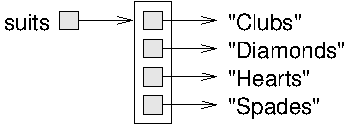
\includegraphics{figs/stringarray.pdf}
\caption{Memory diagram of an array of strings.}
\label{fig.stringarray}
\end{center}
\end{figure}

We also need an array to decode the ranks:

\begin{code}
String[] ranks = {null, "Ace", "2", "3", "4", "5", "6",
           "7", "8", "9", "10", "Jack", "Queen", "King"};
\end{code}

The zeroth element should never be used, because the only valid ranks are 1--13.
We set it to \java{null} to indicate an unused element.

Using these arrays, we can create a meaningful \java{String} by using \java{suit} and \java{rank} as indexes.

\begin{code}
String s = ranks[this.rank] + " of " + suits[this.suit];
\end{code}

The expression \java{ranks[this.rank]} means ``use the instance variable \java{rank} from \java{this} object as an index into the array \java{ranks}.''
We select the string for \java{this.suit} in a similar way.

Now we can wrap all the previous code in a \java{toString} method:

\begin{code}
public String toString() {
    String[] ranks = {null, "Ace", "2", "3", "4", "5", "6",
               "7", "8", "9", "10", "Jack", "Queen", "King"};
    String[] suits = {"Clubs", "Diamonds", "Hearts", "Spades"};
    String s = ranks[this.rank] + " of " + suits[this.suit];
    return s;
}
\end{code}

When we display a card, \java{println} automatically calls \java{toString}.
The output of the following code is {\tt Jack of Diamonds}:

\begin{code}
Card card = new Card(11, 1);
System.out.println(card);
\end{code}


\section{Class Variables}
\label{classvar}

\index{class variable}

So far you have seen local variables, which are declared inside a method, and instance variables, which are declared in a class definition, usually before the method definitions.
Now it's time to learn about {\bf class variables}.
They are shared across all instances of the class.

%Local variables are created when a method is invoked, and their space is reclaimed when the method ends.
%Instance variables are created when you construct an object and reclaimed when the object is garbage-collected.

\index{static}
\index{variable!static}

Like instance variables, class variables are defined in a class definition, before the method definitions.
But they are identified by the keyword \java{static}.
Here is a version of \java{Card} in which \java{RANKS} and \java{SUITS} are defined as class variables:

\begin{code}
public class Card {

    public static final String[] RANKS = {
        null, "Ace", "2", "3", "4", "5", "6", "7",
        "8", "9", "10", "Jack", "Queen", "King"};

    public static final String[] SUITS = {
        "Clubs", "Diamonds", "Hearts", "Spades"};

    // instance variables and constructors go here

    public String toString() {
        return RANKS[this.rank] + " of " + SUITS[this.suit];
    }
}
\end{code}

\index{garbage collection}

Class variables are allocated when the program begins and persist until the program ends.
In contrast, instance variables like \java{rank} and \java{suit} are allocated when the program creates \java{new} objects, and they are deleted when the object is garbage-collected.

% ABD: Let's check whether garbage collection ends up before this.

\index{final}

%You can refer to a class variable from anywhere inside the class definition.
Class variables are often used to store constant values that are needed in several places.
In that case, they should also be declared as \java{final}.
Note that whether a variable is \java{static} or \java{final} involves two separate considerations:
\java{static} means the variable is {\em shared}, and \java{final} means the variable is {\em constant}.

Naming \java{static final} variables with capital letters is a common convention that makes it easier to recognize their role in the class.
In the \java{toString} method, we refer to \java{SUITS} and \java{RANKS} as if they were local variables, but we can tell that they are class variables.

One advantage of defining \java{SUITS} and \java{RANKS} as class variables is that they don't need to be created (and garbage-collected) every time \java{toString} is called.
They may also be needed in other methods and classes, so it's helpful to make them available everywhere.
Since the array variables are \java{final}, and the strings they reference are immutable, there is no danger in making them \java{public}.


\section{The compareTo Method}

\index{equivalent}

As you saw in Section~\ref{equals}, it's helpful to create an \java{equals} method to test whether two objects are equivalent:

\begin{code}
public boolean equals(Card that) {
    return this.rank == that.rank
        && this.suit == that.suit;
}
\end{code}

\index{operator!logical}
\index{logical operator}

It would also be nice to have a method for comparing cards, so we can tell if one is higher or lower than another.
For primitive types, we can use comparison operators like \java{<} and \java{>} to compare values.
But these operators don't work for object types.

For strings, Java provides a \java{compareTo} method, as you saw in Section~\ref{strcmp}.
We can write our own version of \java{compareTo} for the classes that we define, as we did for the \java{equals} method.
%Later we will use this method to sort a deck of cards.

\index{ordering}
\index{complete ordering}
\index{partial ordering}

Some types are ``totally ordered'', which means that you can compare any two values and tell which is bigger.
Integers and strings are totally ordered.
Other types are ``unordered'', which means that there is no meaningful way to say that one element is bigger than another.
In Java, the \java{boolean} type is unordered; if you try to compare \java{true < false}, you get a compiler error.

The set of playing cards is ``partially ordered'', which means that sometimes we can compare cards and sometimes not.
For example, we know that the 3 of Clubs is higher than the 2 of Clubs, and the 3 of Diamonds is higher than the 3 of Clubs.
But which is better, the 3 of Clubs or the 2 of Diamonds?
One has a higher rank, but the other has a higher suit.

\index{compareTo}

To make cards comparable, we have to decide which is more important: rank or suit.
The choice is arbitrary, and it might be different for different games.
But when you buy a new deck of cards, it comes sorted with all the Clubs together, followed by all the Diamonds, and so on.
So for now, let's say that suit is more important.
With that decided, we can write \java{compareTo} as follows:

\begin{code}
public int compareTo(Card that) {
    if (this.suit < that.suit) {
        return -1;
    }
    if (this.suit > that.suit) {
        return 1;
    }
    if (this.rank < that.rank) {
        return -1;
    }
    if (this.rank > that.rank) {
        return 1;
    }
    return 0;
}
\end{code}

\java{compareTo} returns \java{-1} if \java{this} is a lower card, \java{+1} if \java{this} is a higher card, and \java{0} if \java{this} and \java{that} are equivalent.
It compares suits first.
If the suits are the same, it compares ranks.
If the ranks are also the same, it returns \java{0}.


\section{Cards Are Immutable}

The instance variables of \java{Card} are \java{private}, so they can't be accessed from other classes.
We can provide getters to allow other classes to read the \java{rank} and \java{suit} values:

\begin{code}
public int getRank() {
    return this.rank;
}

public int getSuit() {
    return this.suit;
}
\end{code}

\index{immutable}

Whether or not to provide setters is a design decision.
If we did, cards would be mutable, so you could transform one card into another.
That is probably not a feature we want, and in general, mutable objects are more error-prone.
So it might be better to make cards immutable.
To do that, all we have to do is {\em not} provide any modifier methods (including setters).

\index{final}

That's easy enough, but it is not foolproof, because a fool might come along later and add a modifier.
We can prevent that possibility by declaring the instance variables \java{final}:

\begin{code}
public class Card {
    private final int rank;
    private final int suit;

    ...
}
\end{code}

You can initialize these variables inside a constructor,
but if someone writes a method that tries to modify them, they'll get a compiler error.
This kind of safeguard helps prevent future mistakes and hours of debugging.


\section{Arrays of Cards}
\label{cardarray}

%\index{composition}

%By now we have seen several examples of composition; that is, the ability to combine language features in a variety of arrangements.
%One of the first examples we saw was using a method invocation as part of an expression.
%Another example is the nested structure of statements: you can put an \java{if} statement within a \java{while} loop, or within another \java{if} statement, etc.

%Having seen this pattern, and having learned about arrays and objects, you should not be surprised to learn that you can make arrays of objects.
%And you can define objects with arrays as instance variables; you can make arrays that contain arrays; you can define objects that contain objects, and so on.

\index{array!of objects}
\index{object!array of}

Just as you can create an array of \java{String} objects, you can create an array of \java{Card} objects.
The following statement creates an array of 52 cards.
Figure~\ref{fig.cardarray} shows the memory diagram for this array.

\begin{code}
Card[] cards = new Card[52];
\end{code}

\begin{figure}[!ht]
\begin{center}
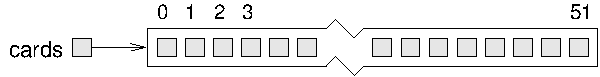
\includegraphics{figs/cardarray.pdf}
\caption{Memory diagram of an unpopulated \java{Card} array.}
\label{fig.cardarray}
\end{center}
\end{figure}

% ABD: I might redraw this to use dashed lines instead of zig-zag to indicate the elided part of the array.

\index{null}

Although we call it an ``array of cards'', the array contains {\em references} to cards; it does not contain the \java{Card} objects themselves.
Initially the references are all \java{null}.

Even so, you can access the elements of the array in the usual way:

\begin{code}
if (cards[0] == null) {
    System.out.println("No card yet!");
}
\end{code}

\index{exception!NullPointer}
\index{run-time error}

But if you try to access the instance variables of non-existent \java{Card} objects, you will get a \java{NullPointerException}:

\begin{code}
System.out.println(cards[0].rank);  // NullPointerException
\end{code}

\index{nesting}
\index{loop!nested}

That code won't work until we put cards in the array.
One way to populate the array is to write nested \java{for} loops:

\begin{code}
int index = 0;
for (int suit = 0; suit <= 3; suit++) {
    for (int rank = 1; rank <= 13; rank++) {
        cards[index] = new Card(rank, suit);
        index++;
    }
}
\end{code}

The outer loop iterates suits from 0 to 3.
For each suit, the inner loop iterates ranks from 1 to 13.
Since the outer loop runs 4 times, and the inner loop runs 13 times for each suit, the body is executed 52 times.

\index{index}

We use a separate variable \java{index} to keep track of where in the array the next card should go.
Figure~\ref{fig.cardarray2} shows what the array looks like after the first two cards have been created.

\begin{figure}[!ht]
\begin{center}
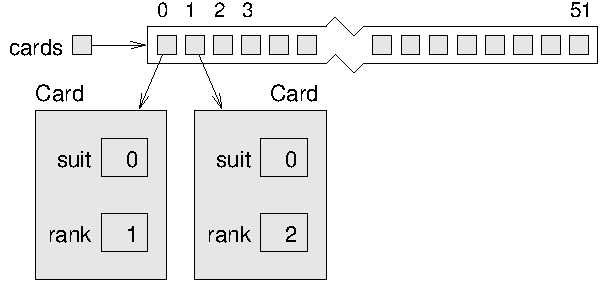
\includegraphics{figs/cardarray2.pdf}
\caption{Memory diagram of a \java{Card} array with two cards.}
\label{fig.cardarray2}
\end{center}
\end{figure}

\index{print!array}

When you work with arrays, it is convenient to have a method that displays the contents.
You have seen the pattern for traversing an array several times, so the following method should be familiar:

% ABD: Maybe add reference to where we introduced enhanced loops?

\begin{code}
public static void printDeck(Card[] cards) {
    for (Card card : cards) {
        System.out.println(card);
    }
}
\end{code}

%\begin{code}
%public static void printDeck(Card[] cards) {
%    for (int i = 0; i < cards.length; i++) {
%        System.out.println(cards[i]);
%    }
%}
%\end{code}

Since \java{cards} has type \java{Card[]}, pronounced ``card array'', an element of \java{cards} has type \java{Card}.
So \java{println} invokes the \java{toString} method in the \java{Card} class.

Then again, we don't have to write our own \java{printDeck} method.
The \java{Arrays} class provides a \java{toString} method that invokes \java{toString} on the elements of an array and concatenates the results:

\begin{code}
System.out.println(Arrays.toString(cards))
\end{code}


\section{Sequential Search}

\index{sequential search}

The next method we'll write is \java{search}, which takes an array of cards and a \java{Card} object as parameters.
It returns the index where the \java{Card} appears in the array, or \java{-1} if it doesn't.
This version of \java{search} uses the algorithm in Section~\ref{traversal}, which is called {\bf sequential search}:

\index{traverse}
\index{loop!search}

\begin{code}
public static int search(Card[] cards, Card target) {
    for (int i = 0; i < cards.length; i++) {
        if (cards[i].equals(target)) {
            return i;
        }
    }
    return -1;
}
\end{code}

\index{statement!return}
\index{return!inside loop}

The method returns as soon as it discovers the card, which means we don't have to traverse the entire array if we find the target.
If we get to the end of the loop, we know the card is not in the array.

\index{efficiency}

If the cards in the array are not in order, there is no way to search faster than sequential search.
We have to look at every card, because otherwise we can't be certain the card we want is not there.
But if the cards are in order, we can use better algorithms.

Sequential search is relatively inefficient, especially for large arrays.
If you pay the price to keep the array sorted, finding elements becomes much easier.
%We will learn in the next chapter how to sort arrays.


\section{Binary Search}

% ABD:  I wonder if we need a different example.  I don't know how many students have looked up a word in a paper dictionary.

\index{binary search}

When you look for a word in a dictionary, you don't search page by page from front to back.
Since the words are in alphabetical order, you probably use a {\bf binary search} algorithm:

\begin{enumerate}

\item Start on a page near the middle of the dictionary.

\item Compare a word on the page to the word you are looking for.
If you find it, stop.

\item If the word on the page comes before the word you are looking for, flip to somewhere later in the dictionary and go to step 2.

\item If the word on the page comes after the word you are looking for, flip to somewhere earlier in the dictionary and go to step 2.

\end{enumerate}

This algorithm is much faster than sequential search, because it rules out half of the remaining words each time you make a comparison.
If at any point you find two adjacent words on the page, and your word comes between them, you can conclude that your word is not in the dictionary.

Getting back to the array of cards, we can write a faster version of \java{search} if we know the cards are in order:

\begin{code}
public static int binarySearch(Card[] cards, Card target) {
    int low = 0;
    int high = cards.length - 1;
    while (low <= high) {
        int mid = (low + high) / 2;                 // step 1
        int comp = cards[mid].compareTo(target);

        if (comp == 0) {                            // step 2
            return mid;
        } else if (comp < 0) {                      // step 3
            low = mid + 1;
        } else {                                    // step 4
            high = mid - 1;
        }
    }
    return -1;
}
\end{code}

First, we declare \java{low} and \java{high} variables to represent the range we are searching.
Initially, we search the entire array, from \java{0} to \java{cards.length - 1}.

Inside the \java{while} loop, we repeat the four steps of binary search:

\begin{enumerate}

\item Choose an index between \java{low} and \java{high}---call it \java{mid}---and compare the card at \java{mid} to the target.

\item If you found the target, return its index (which is \java{mid}).

\item If the card at \java{mid} is lower than the target, search the range from \java{mid + 1} to \java{high}.

\item If the card at \java{mid} is higher than the target, search the range from \java{low} to \java{mid - 1}.

\end{enumerate}

If \java{low} exceeds \java{high}, there are no cards in the range, so we terminate the loop and return \java{-1}.

This algorithm depends on only the \java{compareTo} method of the object, so we can use this code with any object type that provides \java{compareTo}.


\section{Tracing the Code}

\index{tracing}

To see how binary search works, it's helpful to add the following print statement at the beginning of the loop:

\begin{code}
System.out.println(low + ", " + high);
\end{code}

Using a sorted deck of cards, we can search for the Jack of Clubs like this:

\begin{code}
Card card = new Card(11, 0);
System.out.println(binarySearch(cards, card));
\end{code}

We expect to find this card at position 10 (since the Ace of Clubs is at position 0).
Here is the output of \java{binarySearch}:

\begin{stdout}
0, 51
0, 24
0, 11
6, 11
9, 11
10
\end{stdout}

You can see the range of cards shrinking as the \java{while} loop runs, until eventually index 10 is found.
If we search for a card that's not in the array---like \java{new Card(15, 1)}, or the 15 of Diamonds---we get the following:

\begin{stdout}
0, 51
26, 51
26, 37
26, 30
26, 27
-1
\end{stdout}

%\index{testing}
%\index{correctness}
%
%These tests don't prove that this program is correct.
%In fact, no amount of testing can {\em prove} that a program is correct.
%But looking at a few cases and examining the code, you might be able to convince yourself.

Each time through the loop, we cut the distance between \java{low} and \java{high} in half.
After $k$ iterations, the number of remaining cards is $52 / 2^k$.
To find the number of iterations it takes to complete, we set $52 / 2^k = 1$ and solve for $k$.
The result is $\log_2 52$, which is about 5.7.
So we might have to look at 5 or 6 cards, as opposed to all 52 if we did a sequential search.

More generally, if the array contains $n$ elements, binary search requires $\log_2 n$ comparisons, and sequential search requires $n$.
For large values of $n$, binary search is substantially faster.


\section{Vocabulary}

\begin{description}

\term{encode}
To represent one set of values using another set of values by constructing a mapping between them.

\term{class variable}
A variable declared within a class as \java{static}.
There is only one copy of a class variable, no matter how many objects there are.

\term{sequential search}
An algorithm that searches array elements, one by one, until a target value is found.

\term{binary search}
An algorithm that searches a sorted array by starting in the middle, comparing an element to the target, and eliminating half of the remaining elements.

\end{description}


\section{Exercises}

The code for this chapter is in the {\it ch12} directory of {\it ThinkJavaCode2}.
See page~\pageref{code} for instructions on how to download the repository.
Before you start the exercises, we recommend that you compile and run the examples.

%TODO make an exercise of validating the input to Card constructor?


\begin{exercise}  %%V6 Ex12.1

Encapsulate the deck-building code from Section~\ref{cardarray} in a method called \java{makeDeck} that takes no parameters and returns a fully populated array of \java{Card}s.

\end{exercise}


\begin{exercise}  %%V6 Ex12.2

In some card games, Aces are ranked higher than Kings.
Modify the \java{compareTo} method to implement this ordering.

\end{exercise}


\begin{exercise}  %%V6 Ex12.3

In Poker a ``flush'' is a hand that contains five or more cards of the same suit.
A hand can contain any number of cards.

\index{histogram}

\begin{enumerate}

\item Write a method called \java{suitHist} that takes an array of cards as a parameter and returns a histogram of the suits in the hand.
Your solution should traverse the array only once, as in Section~\ref{singlepass}.

\item Write a method called \java{hasFlush} that takes an array of cards as a parameter and returns \java{true} if the hand contains a flush (and \java{false} otherwise).

\item A ``royal flush'' includes the Ace, King, Queen, Jack, and 10 (all in the same suit). Write a method called \java{hasRoyal} that determines whether an array of cards contains a royal flush.

\end{enumerate}
\vspace{0pt}

\end{exercise}


\begin{exercise}  %%V6 Ex12.4

% ABD: I have a mild preference for 2-D rather than 2D.  Worth changing?

Working with cards is more fun if you can display them on the screen.
If you have not already read Appendix~\ref{graphics} about 2D graphics, you should read it before working on this exercise.
In the code directory for this chapter, {\it ch12}, you will find the following:

\begin{itemize}

\item {\it cardset-oxymoron} \\ A directory containing images of playing cards.

\item {\it CardTable.java} \\ A sample program that demonstrates how to read and display images.

\end{itemize}

\index{array!2D}

{\it CardTable.java} demonstrates the use of a 2D array; specifically, an array of card images.
The declaration looks like this:

\begin{code}
private Image[][] images;
\end{code}

The variable \java{images} refers to a 2D array of \java{Image} objects, which are defined in the \java{java.awt} package.
Here's the code that creates the array itself:

\begin{code}
images = new Image[14][4];
\end{code}

The array has 14 rows (one for each rank, plus an unused row for rank 0) and 4 columns (one for each suit).
Here's the loop that populates the array:

\begin{code}
String cardset = "cardset-oxymoron";
String suits = "cdhs";

for (int suit = 0; suit <= 3; suit++) {
    char c = suits.charAt(suit);

    for (int rank = 1; rank <= 13; rank++) {
        String s = String.format("%s/%02d%c.gif",
                                 cardset, rank, c);
        images[rank][suit] = new ImageIcon(s).getImage();
    }
}
\end{code}

The variable \java{cardset} contains the name of the directory that contains the image files.
\java{suits} is a string that contains the single-letter abbreviations for the suits.
These strings are used to assemble \java{s}, which contains the filename for each image.
For example, when \java{rank=1} and \java{suit=2}, the value of \java{s} is \java{"cardset-oxymoron/01h.gif"}, which is an image of the Ace of Hearts.

The last line of the loop reads the image file, extracts an \java{Image} object, and assigns it to a location in the array, as specified by the indexes \java{rank} and \java{suit}.
For example, the image of the Ace of Hearts is stored in row 1, column 2.

If you compile and run {\it CardTable.java}, you should see images of a deck of cards laid out on a green table.
You can use this class as a starting place to implement your own card games.

% TODO: ML suggests including a screen shot

%TODO We should make an actual exercise out of this.
% Maybe take an array of cards and display them in a row at a given location?

As a starting place, try placing cards on the table in the starting configuration for the solitaire game Klondike (\url{https://en.wikipedia.org/wiki/Klondike_(solitaire)}).

You can get the image for the back of the card by reading the file {\it back192.gif}.

\end{exercise}


\chapter{Objects of arrays}

\index{array!of cards}

In the previous chapter, we defined a class to represent cards and used an array of \java{Card} objects to represent a deck.
In this chapter, we take another step toward object-oriented programming by defining a class to represent a deck of cards.
We also present algorithms for shuffling and sorting decks.
Finally, we introduce \java{ArrayList} from the Java library and use it to keep track of which cards each player has from the deck.

%While reading the following sections, we recommend that you create a {\tt Deck.java} file and paste in all the examples.
%You will need {\tt Card.java} from the previous chapter for it to compile.

%So many of the examples are non-idiomatic; that is, they are not good Java.
%This transitional form should help you learn, but don't write code like this.

%The code for this chapter is in {\tt Card.java} and {\tt Deck.java}, which are in the directory {\tt ch13} in the repository for this book.
%Instructions for downloading this code are on page~\pageref{code}.


\section{The Deck class}
\label{deck}

The first goal of this chapter is to create a \java{Deck} class that encapsulates an array of \java{Card}s.
The initial class definition looks like this:

\begin{code}
public class Deck {
    private Card[] cards;

    public Deck(int n) {
        this.cards = new Card[n];
    }
    
    public Card[] getCards() {
        return this.cards;
    }
}
\end{code}

\index{constructor}
\index{memory diagram}
\index{diagram!memory}

The constructor initializes the instance variable with an array of \java{n} cards, but it doesn't create any \java{Card} objects.
Figure~\ref{fig.deckobject} shows what a \java{Deck} looks like with no cards.

\begin{figure}[!ht]
\begin{center}
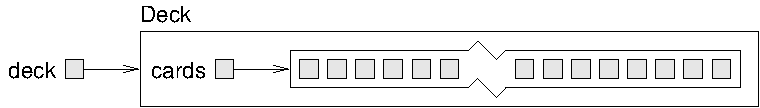
\includegraphics{figs/deckobject.pdf}
\caption{Memory diagram of an unpopulated \java{Deck} object.}
\label{fig.deckobject}
\end{center}
\end{figure}

We'll add another constructor that creates a standard 52-card array and populates it with \java{Card} objects:

\begin{code}
public Deck() {
    this.cards = new Card[52];
    int index = 0;
    for (int suit = 0; suit <= 3; suit++) {
        for (int rank = 1; rank <= 13; rank++) {
            this.cards[index] = new Card(rank, suit);
            index++;
        }
    }
}
\end{code}

This method is similar to the example in Section~\ref{cardarray}; we just turned it into a constructor.
We can now create a standard \java{Deck} like this:

\begin{code}
Deck deck = new Deck();
\end{code}

\index{printDeck}

Now that we have a \java{Deck} class, we have a logical place to put methods that pertain to decks.
Looking at the methods we have written so far, one obvious candidate is \java{printDeck} from Section~\ref{cardarray}.
Here's how it looks, rewritten as an instance method of \java{Deck}:

\begin{code}
public void print() {
    for (Card card : this.cards) {
        System.out.println(card);
    }
}
\end{code}

%\begin{code}
%public void print() {
%    for (int i = 0; i < this.cards.length; i++) {
%        System.out.println(this.cards[i]);
%    }
%}
%\end{code}

Notice that when you transform a static method into an instance method, the code is shorter.
We can simply type \java{deck.print()} to invoke this method.


\section{Shuffling decks}
\label{shuffle}

\index{shuffle}

For most card games, you need to be able to shuffle the deck; that is, put the cards in a random order.
In Section~\ref{random} we saw how to generate random numbers, but it is not obvious how to use them to shuffle a deck.

One possibility is to model the way humans shuffle, which is usually dividing the deck in two halves and then choosing alternately from each one.
Since humans usually don't shuffle perfectly, after about seven iterations the order of the deck is pretty well randomized.

But a computer program would have the annoying property of doing a perfect shuffle every time, which is not very random.
In fact, after eight perfect shuffles, you would find the deck back in the order you started in!
For more on this, see \url{https://en.wikipedia.org/wiki/Faro_shuffle}.

\index{pseudocode}

A better shuffling algorithm is to traverse the deck one card at a time, and at each iteration, choose two cards and swap them.
Here is an outline of how this algorithm works.
To sketch the method, we will use a combination of Java statements and English.
This technique is sometimes called {\bf pseudocode}.

\index{shuffle}

\begin{code}
public void shuffle() {
    for each index i {
        // choose a random number between i and length - 1
        // swap the ith card and the randomly-chosen card
    }
}
\end{code}

\index{helper method}
\index{method!helper}

The nice thing about pseudocode is that it often makes clear what other methods you are going to need.
In this case, we need a method that chooses a random integer between \java{low} and \java{high}, and a method that takes two indexes and swaps the cards at those positions.

\begin{code}
private static int randomInt(int low, int high) {
    // return a random number between low and high
}

private void swapCards(int i, int j) {
    // swap the ith and the jth cards in the array
}
\end{code}

\index{randomInt}
\index{swapCards}

Methods like \java{randomInt} and \java{swapCards} are called {\bf helper methods}, because they help you solve parts of the problem.
Helper methods are often \java{private}, since they are specific to the internal details of the class.

\index{top-down design}
\index{design process}

This process of writing pseudocode first and then writing helper methods to make it work is called {\bf top-down design} (see \url{https://en.wikipedia.org/wiki/Top-down_and_bottom-up_design}).
It is similar to ``incremental development'' and ``encapsulation and generalization'', the other design processes we have seen so far.

One of the exercises at the end of the chapter asks you to write the helper methods \java{randomInt} and \java{swapCards}, and use them to implement \java{shuffle}.


\section{Selection sort}
\label{sorting}

\index{selection sort}
\index{sort!selection}

Now that we have shuffled the deck, we need a way to put it back in order.
There is an algorithm for sorting that is ironically similar to the algorithm for shuffling.
It's called {\bf selection sort}, because it works by traversing the array repeatedly and selecting the lowest (or highest) remaining card each time.

During the first iteration, we find the lowest card and swap it with the card in the 0th position.
During the $i$th iteration, we find the lowest card to the right of $i$ and swap it with the $i$th card.
%Here is pseudocode for selection sort:

\begin{code}
public void selectionSort() {
    for each index i {
        // find the lowest card at or to the right of i
        // swap the ith card and the lowest card found
    }
}
\end{code}

Again, the pseudocode helps with the design of the helper methods.
For this algorithm we can use \java{swapCards} from before, so we only need a method to find the lowest card; we'll call it \java{indexLowest}.

\begin{code}
private int indexLowest(int low, int high) {
    // find the lowest card between low and high
}
\end{code}


One of the exercises at the end of the chapter asks you to write the helper method \java{indexLowest}; use it and \java{swapCards} to implement \java{selectionSort}.


\section{Merge sort}
\label{mergesort}

\index{efficiency}

Selection sort is a simple algorithm, but it is not very efficient.
To sort $n$ items, it has to traverse the array $n-1$ times.
Each traversal takes an amount of time proportional to $n$.
The total time, therefore, is proportional to $n^2$.

\index{merge sort}
\index{sort!merge}

In the next two sections, we'll develop a more efficient algorithm called {\bf merge sort}.
To sort $n$ items, merge sort takes time proportional to $n \log_2 n$.
That may not seem impressive, but as $n$ gets big, the difference between $n^2$ and $n \log_2 n$ can be enormous.

For example, $\log_2$ of one million is around 20.
So if you had to sort a million numbers, merge sort would require 20 million steps.
But selection sort would require one trillion!

The idea behind merge sort is this: if you have two subdecks, each of which has already been sorted, it is easy and fast to merge them into a single, sorted deck.
Try this out with a deck of cards:

\begin{enumerate}

\item Form two subdecks with about 10 cards each, and sort them so that when they are face up the lowest cards are on top.
Place both decks face up in front of you.

\item Compare the top card from each deck and choose the lower one.
Flip it over and add it to the merged deck.

\item Repeat step 2 until one of the decks is empty.
Then take the remaining cards and add them to the merged deck.

\end{enumerate}

The result should be a single sorted deck.
In the next few sections, we'll explain how to implement this algorithm in Java.


\section{Subdecks}

\index{subdeck}

The first step of merge sort is to split the deck into two subdecks, each with about half of the cards.
So we need to write a method, \java{subdeck}, that takes a deck and a range of indexes.
It returns a new deck that contains the specified subset of the cards.

\begin{code}
public Deck subdeck(int low, int high) {
    Deck sub = new Deck(high - low + 1);
    for (int i = 0; i < sub.cards.length; i++) {
        sub.cards[i] = this.cards[low + i];
    }
    return sub;
}
\end{code}

The first line creates an unpopulated subdeck (an array of \java{null} references).
Inside the \java{for} loop, the subdeck gets populated with references from the deck.

\index{off-by-one}

The length of the subdeck is \java{high - low + 1}, because both the low card and the high card are both included.
This sort of computation can be confusing, and forgetting the ``\java{+ 1}'' often leads to {\bf off-by-one} errors.
Drawing a picture is usually the best way to avoid them.

%For example, to select the middle three of five values in an array, we need \java{3 - 1 + 1} values.
%
%\begin{center}
%\begin{tabular}{ccccc}
%\hline
%\multicolumn{1}{|c|}{} & \multicolumn{1}{c|}{X} & \multicolumn{1}{c|}{X} & \multicolumn{1}{c|}{X} & \multicolumn{1}{c|}{} \\
%\hline
%0                      & 1                      & 2                      & 3                      & 4                     \\
%\end{tabular}
%\end{center}

\index{constructor}
\index{overload}

Figure~\ref{fig.subdeck} is a memory diagram of a subdeck with \java{low = 0} and \java{high = 4}.
The result is a hand with five cards that are {\em shared} with the original deck; that is, they are aliased.

\begin{figure}[!ht]
\begin{center}
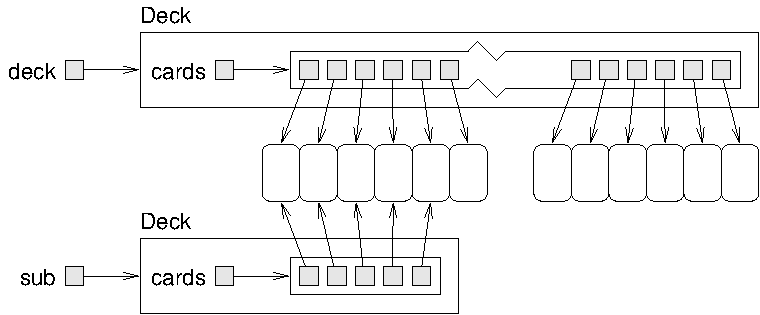
\includegraphics{figs/subdeck.pdf}
\caption{Memory diagram showing the effect of \java{subdeck}.}
\label{fig.subdeck}
\end{center}
\end{figure}

\index{aliasing}
\index{reference}

Aliasing might not be a good idea, because changes to shared cards would be reflected in multiple decks.
But since \java{Card} objects are immutable, this kind of aliasing is not a problem at all.
It also saves a lot of memory, because we never have to create duplicate \java{Card} objects.


\section{Merging decks}

The next helper method we need is \java{merge}, which takes two sorted subdecks and returns a new deck containing all cards from both decks, in order.
Here's what the algorithm looks like in pseudocode, assuming the subdecks are named \java{d1} and \java{d2}:

\begin{code}
private static Deck merge(Deck d1, Deck d2) {
    // create a new deck big enough for all the cards

    // use the index i to keep track of where we are at in
    // the first deck, and the index j for the second deck
    int i = 0;
    int j = 0;

    // the index k traverses the result deck
    for (int k = 0; k < d3.length; k++) {

        // if d1 is empty, use top card from d2
        // if d2 is empty, use top card from d1
        // otherwise, compare the top two cards

        // add lowest card to the new deck at k
        // increment i or j (depending on card)
    }
    // return the new deck
}
\end{code}

An exercise at the end of the chapter asks you to implement \java{merge}.
It's somewhat tricky, so be sure to test it with different subdecks.
Once your \java{merge} method is working corectly, you can use it to write a simplified version of merge sort:

\begin{code}
public Deck almostMergeSort() {
    // divide the deck into two subdecks
    // sort the subdecks using selectionSort
    // merge the subdecks, return the result
}
\end{code}


\section{Adding recursion}

Now that we have a way to \java{merge} two decks, the real fun begins!
The magical thing about merge sort is that it is inherently recursive.
Take another look at the pseudocode for \java{almostMergeSort} in the previous section.

At the point where you sort the subdecks, why should you invoke the slower method, \java{selectionSort}?
Why not invoke the spiffy new \java{mergeSort} method, the one you are in the process of writing?
Not only is that a good idea, it is {\em necessary} to achieve the $\log_2$ performance advantage.
\index{recursion}

To make \java{mergeSort} work recursively, you have to add a base case; otherwise it repeats forever.
A simple base case is a subdeck with 0 or 1 cards.
If \java{mergeSort} receives such a small subdeck, it can return it unmodified since it would already be sorted.

The recursive version of \java{mergeSort} looks something like this:

\begin{code}
public Deck mergeSort() {
    // if the deck has 0 or 1 cards, return it
    // divide the deck into two subdecks
    // sort the subdecks using mergeSort
    // merge the subdecks, return the result
}
\end{code}

\index{leap of faith}

As usual, there are two ways to think about recursive programs: you can think through the entire flow of execution, or you can make the ``leap of faith'' (see Section~\ref{leap_of_faith}).
This example might encourage you to make the leap of faith.

When you used \java{selectionSort} to sort the subdecks, you didn't feel compelled to follow the flow of execution.
You just assumed it works because you had already debugged it.
And all you did to make \java{mergeSort} recursive was replace one sorting algorithm with another.
There is no reason to read the program any differently.

Well, almost.
You might have to give some thought to getting the base case right and making sure that you reach it eventually.
But other than that, writing the recursive version should be no problem.


\section{Static context}

Figure~\ref{fig.deck} lists the methods we have discussed.
In UML diagrams, \java{private} methods begin with a minus sign (\java{-}), and \java{static} methods are underlined.

\begin{figure}[!ht]
\begin{center}
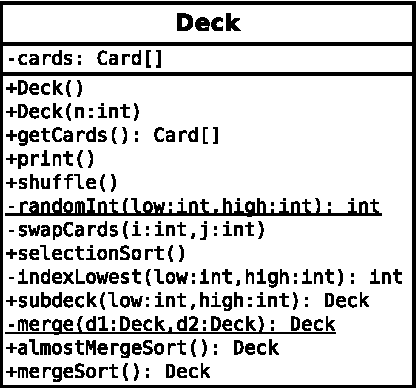
\includegraphics{figs/deck.pdf}
\caption{UML diagram for the \java{Deck} class.}
\label{fig.deck}
\end{center}
\end{figure}

The helper methods \java{randomInt} and \java{merge} are \java{static}, because they do not require \java{this.cards}.
All other methods are instance methods, because they require a specific instance of \java{this.cards}.
For example, you cannot invoke the \java{print} method this way:

\begin{code}
Deck.print();  // wrong!
\end{code}

\index{static context}
\index{this}

If you try to compile this code, you will get the error, ``non-static method print() cannot be referenced from a static context.''
By {\bf static context}, the compiler means you are trying to invoke a method without \java{this}.
To invoke an instance method, you need an instance:

\begin{code}
Deck deck = new Deck();
deck.print();  // correct
\end{code}

Notice that \java{Deck} with a capital \java{D} is a class, and \java{deck} with a lowercase \java{d} is a variable.
When you invoke \java{deck.print()}, the reference of \java{deck} becomes the reference \java{this}.
Static methods cannot refer to \java{this}, because they are not bound to a specific object.

\begin{code}
private static Deck merge(Deck d1, Deck d2) {
    return this.cards;  // wrong!
}
\end{code}

If you refer to \java{this} in a static method, you will get the compiler error, ``non-static variable this cannot be referenced from a static context.''
In static methods, there is no such thing as \java{this}.

\index{sort!Arrays}
\index{array!sorting}

Normally, we wouldn't implement three different sorting algorithms in the same class.
Our goal with \java{Deck} was to demonstrate different ways of solving the same problem.
In practice, we could just write a single \java{sort} method that uses \java{java.util.Arrays}.

\begin{code}
public void sort() {
    Arrays.sort(this.cards);
}
\end{code}

%%V6 Ex13.1
You can learn more about the sorting algorithms in this chapter, and others, at \href{http://www.sorting-algorithms.com/}{sorting-algorithms.com}.
This site includes explanations of the algorithms, animations that show how they work, and analysis of their efficiency.


\section{Piles of cards}

Now that we have a working \java{Deck} class, let's use it to implement a simple card game.
One of the simplest games that children often play is ``War'' (see \url{https://en.wikipedia.org/wiki/War_(card_game)}).

In this game, the deck is divided into two or more piles.
Players take turns revealing the top card of their pile.
If there is a tie, players set aside three more cards and reveal their next card.
Whoever has the highest ranking card takes all the cards that were played.
The game continues until one player has won the entire deck.

We could use the \java{Deck} class to represent the individual piles.
However, our implementation of \java{Deck} uses a \java{Card} array, and the length of an array can't change.
As the game progresses, we need to be able to add and remove cards from the piles.

\index{ArrayList}
\index{collection}

We can solve this problem by using an \java{ArrayList}, which is in the \java{java.util} package.
An \java{ArrayList} is a {\bf collection}, which is an object that contains other objects.
It provides methods to add and remove elements, and it grows and shrinks automatically.

%The Java library includes many other collections (see \url{https://docs.oracle.com/javase/8/docs/technotes/guides/collections/}).
%For our purposes, \java{ArrayList} is a good choice because it provides methods to add and remove elements, and it grows and shrinks automatically.

We will define a new class named \java{Pile} that represents a pile of cards.
It uses an \java{ArrayList} (instead of an array) to store the \java{Card} objects.

\begin{code}
public class Pile {
    private ArrayList<Card> cards;

    public Pile() {
        this.cards = new ArrayList<Card>();
    }
}
\end{code}

\index{angle brackets}

When you declare an \java{ArrayList}, you specify the type it contains in angle brackets (\java{<>}).
This declaration says that \java{cards} is not just an \java{ArrayList}, it's an \java{ArrayList} of \java{Card} objects.
The constructor initializes \java{this.cards} with an empty \java{ArrayList}.

%Java collections can only store objects, not primitives like \java{int}.
%But you can use wrapper classes, for example \java{ArrayList<Integer>}.

\java{ArrayList} provides a method, \java{add}, that adds an element to the collection.
We will write a \java{Pile} method that does the same thing:

\begin{code}
public void addCard(Card card) {
    this.cards.add(card);        // to the bottom of the pile
}
\end{code}

\index{this}

We also need to be able to remove cards from ``the top'' of the pile.
If we use \java{ArrayList.remove}, it will automatically shift the remaining cards left to fill the gap.

\begin{code}
public Card popCard() {
    return this.cards.remove(0);  // from the top of the pile
}
\end{code}

In order to know when to stop the game, we need to know how many cards are in each pile.

\begin{code}
public int size() {
    return this.cards.size();
}
\end{code}

\index{wrapper method}

Methods like \java{addCard}, \java{popCard}, and \java{size}, which invoke another method without doing much additional work, are called {\bf wrapper methods}.
The last method we need adds an entire subdeck at the beginning of the game.

\begin{code}
public void addDeck(Deck deck) {
    for (Card card : deck.getCards()) {
        this.cards.add(card);
    }
}
\end{code}

Now we can use \java{Deck} and \java{Pile} to implement the game.
In \java{War.java}, the \java{main} method begins like this:

\begin{code}
// create and shuffle the deck
Deck deck = new Deck();
deck.shuffle();

// divide the deck into piles
Pile p1 = new Pile();
p1.addDeck(deck.subdeck(0, 25));
Pile p2 = new Pile();
p2.addDeck(deck.subdeck(26, 51));
\end{code}

The game itself is a loop that repeats until one of the piles is empty.
At each iteration, we draw a card from each pile and compare their ranks.

\begin{code}
// while both piles are not empty
while (p1.size() > 0 && p2.size() > 0) {
    Card c1 = p1.popCard();
    Card c2 = p2.popCard();
    
    // compare the cards
    int diff = c1.getRank() - c2.getRank();
    if (diff > 0) {
        p1.addCard(c1);
        p1.addCard(c2);
    } else if (diff < 0) {
        p2.addCard(c1);
        p2.addCard(c2);
    } else {  // it's a tie...draw three more cards
\end{code}

One of the exercises at the end of this chapter asks you to implement the \java{else} block when there's a tie.
After the \java{while} loop ends, we display the winner based on which pile is not empty.

\begin{code}
if (p1.size() > 0) {
    System.out.println("Player 1 wins!");
} else {
    System.out.println("Player 2 wins!");
}
\end{code}

\java{ArrayList} provides many other methods that we didn't use for this example program.
You can read about them in the documentation, which you can find by doing a web search for ``Java ArrayList''.


\section{Vocabulary}

\begin{description}

\term{pseudocode}
A way of designing programs by writing rough drafts in a combination of English and Java.

\term{helper method}
Often a small method that does not do anything enormously useful by itself, but which helps another, more complex method.

\term{top-down design}
Breaking down a problem into sub-problems, and solving each sub-problem one at a time.

\term{selection sort}
A simple sorting algorithm that searches for the smallest or largest element $n$ times.

\term{merge sort}
A recursive sorting algorithm that divides an array into two parts, sorts each part (using merge sort), and merges the results.

\term{off-by-one}
A common programming mistake that results in iterating one too few (or too many) times.

%\term{insertion sort}
%Another sorting algorithm that inserts elements into place, one at a time.

\term{static context}
The parts of a class that run without reference to a specific instance of the class.

\term{collection}
An object that contains other objects, or more specifically, one of the objects in the Java library, like \java{ArrayList}, that contains objects.

\term{wrapper method}
A method that calls another method without doing much additional work.

\end{description}


\section{Exercises}

The code for this chapter is in the {\tt ch13} directory of {\tt ThinkJavaCode2}.
See page~\pageref{code} for instructions on how to download the repository.
Before you start the exercises, we recommend that you compile and run the examples.


\begin{exercise}  %%V6 Ex13.5

Write a \java{toString} method for the \java{Deck} class.
It should return a single string that represents the cards in the deck.
When it's printed, this string should display the same results as the \java{print} method in Section~\ref{deck}.

\index{StringBuilder}
\index{efficiency}

{\it Hint:} You can use the \java{+} operator to concatenate strings, but it is not very efficient.
Consider using \java{java.lang.StringBuilder} instead; you can review the documentation by doing a web search for ``Java StringBuilder''.

\end{exercise}


\begin{exercise}  %%V6 Ex13.2
\label{ex.shuffle}

The goal of this exercise is to implement the shuffling algorithm from this chapter.

\begin{enumerate}

\item In the repository for this book, you should find a file called {\tt Deck.java} that contains the code in this chapter.
Check that you can compile it in your environment.

\item Add a \java{Deck} method called \java{randomInt} that takes two integers, \java{low} and \java{high}, and returns a random integer between \java{low} and \java{high}, including both.
You can use the \java{nextInt} provided by \java{java.util.Random}, which we saw in Section~\ref{random}.

{\it Hint:} You can avoid creating a \java{Random} object every time \java{randomInt} is invoked by defining and using a class variable.


\item Write a method called \java{swapCards} that takes two indexes and swaps the cards at the given locations.

\item Write a method called \java{shuffle} that uses the algorithm in Section~\ref{shuffle}.

\end{enumerate}

\end{exercise}


\begin{exercise}  %%V6 Ex13.3

The goal of this exercise is to implement the sorting algorithms from this chapter.
Use the {\tt Deck.java} file from the previous exercise (or create a new one from scratch).

\begin{enumerate}

\item Write a method called \java{indexLowest} that uses the \java{compareCard} method to find the lowest card in a given range of the deck (from \java{lowIndex} to \java{highIndex}, including both).

\item Write a method called \java{selectionSort} that implements the selection sort algorithm in Section~\ref{sorting}.

\item Using the pseudocode in Section~\ref{mergesort}, write the method called \java{merge}.
The best way to test it is to build and shuffle a deck.
Then use \java{subdeck} to form two small subdecks, and use selection sort to sort them.
Then you can pass the two halves to \java{merge} to see if it works.
\index{testing}

\item Write the simple version of \java{mergeSort}, the one that divides the deck in half, uses \java{selectionSort} to sort the two halves, and uses \java{merge} to create a new, sorted deck.

\item Write a recursive version of \java{mergeSort}.
Remember that \java{selectionSort} is a modifier and \java{mergeSort} is a pure method, which means that they get invoked differently:

\begin{code}
deck.selectionSort();      // modifies an existing deck
deck = deck.mergeSort();   // replaces old deck with new
\end{code}

\end{enumerate}

\end{exercise}


\begin{exercise}  %%V6 Ex13.4

The goal of this exercise is to practice top-down design.
First read about ``insertion sort'' at \url{http://www.sorting-algorithms.com/insertion-sort}.
Then write a method named \java{insertionSort} that implements this algorithm.
Your method should use at least one helper method.

\end{exercise}


\begin{exercise}  %%V6.5 NEW

Open the file \java{War.java} in the repository.
The \java{main} method contains all the code from the last section of this chapter.
Check that you can compile and run this code before proceeding.

The program is incomplete; it does not handle the case when two cards have the same rank.
Finish implementing the \java{main} method beginning at the line that says: \java{// it's a tie...draw three more cards}.

When there's a tie, you need to draw three cards from each pile and store them in another collection.
Then draw one more card from each pile and compare them.
Whoever wins the tie will take all eight of these cards.

If one pile does not have at least four cards, the game ends immediately.
If a tie ends with a tie, flip a coin and give the cards to one of the players.

Notice that the program depends on \java{Deck.shuffle}.
If you haven't implemented the \java{shuffle} method (see Exercise~\ref{ex.shuffle}), every play will be a tie.
Player 1 will have the Ace through King of the first two suits, and Player 2 will have the the Ace through King of the remaining two suits, all in the same order.
As a result, the winner will be random.

\end{exercise}


\begin{exercise}  %%V6.5 NEW

Extend your program from the previous exercise to handle the case when a tie ends with a tie.
In other words, when the fourth cards have the same rank, add three more cards to the collection and try again.
You will need to wrap your code in a loop, for example: \java{while (diff == 0)}.

\end{exercise}


\chapter{Objects of objects}
\label{eights}

\index{Crazy Eights}

Now that we have classes that represent cards and decks, let's use them to make a game!
{\it Crazy Eights} is a classic card game for two or more players.
The main objective is to be the first player to get rid of all your cards.
Here's how to play:

\begin{itemize}

\item Deal five or more cards to each player, and then deal one card face up to create the ``discard pile''.
Place the remaining cards face down to create the ``draw pile''.

\item Each player takes turns placing a single card on the discard pile.
The card must match the rank or suit of the previously played card, or be an eight, which is a ``wild card''.

\item When players don't have a matching card or an eight, they must draw new cards until they get one.

\item If the draw pile ever runs out, the discard pile is shuffled (except the top card) and becomes the new draw pile.

\item As soon as a player has no cards, the game ends and all other players score penalty points for their remaining cards.
Eights are worth 20, face cards are worth 10, and all others are worth their rank.

\end{itemize}

You can read \url{https://en.wikipedia.org/wiki/Crazy_Eights} for more details, but we have enough to get started.

The code for this chapter is in the directory {\tt ch14} in the repository for this book.
Instructions for downloading this code are on page~\pageref{code}.


\section{Decks and hands}

To implement this game, we need to represent a deck of cards, a discard pile, a draw pile, and a hand for each player.
And we need to be able to deal, draw, and discard cards.

The \java{Deck} class from the previous chapter meets some of these requirements, but there are two problems:

\begin{itemize}

\item Hands and piles have different sizes, and their sizes change as the game progresses.
Our implementation of \java{Deck} uses a \java{Card} array, and the size of an array can't change.

\item It's not clear that a \java{Deck} object is the right way to represent hands and piles.
We might want new classes for other collections of cards.

\end{itemize}

\index{ArrayList}
\index{collection}

We can solve the first problem by replacing the \java{Card} array with an \java{ArrayList}, which is in the \java{java.util} package.
An \java{ArrayList} is a {\bf collection}, which is an object that contains other objects.

The Java library provides a variety of collections.
For our purposes, \java{ArrayList} is a good choice because it provides methods to add and remove elements, and it grows and shrinks automatically.

\index{inheritance}

To solve the second problem, we can use a language feature called {\bf inheritance}.
We'll define a new class, \java{CardCollection}, to represent a collection of cards.
Then we'll define \java{Deck} and \java{Hand} as subclasses of \java{CardCollection}.

\index{subclass}
\index{extends}

A {\bf subclass} is a new class that ``extends'' an existing class; that is, it has the attributes and methods of the existing class, plus more.
We'll see the details soon, but let's start with \java{CardCollection}:


\section{CardCollection}

Here's the beginning of a \java{CardCollection} class that uses \java{ArrayList} instead of a primitive array:

\begin{code}
public class CardCollection {

    private String label;
    private ArrayList<Card> cards;

    public CardCollection(String label) {
        this.label = label;
        this.cards = new ArrayList<Card>();
    }
}
\end{code}

\index{angle brackets}

When you declare an \java{ArrayList}, you specify the type it contains in angle brackets (\java{<>}).
This declaration says that \java{cards} is not just an \java{ArrayList}, it's an \java{ArrayList} of \java{Card} objects.

%Java collections can only store objects, not primitives like \java{int}.
%But you can use wrapper classes, for example \java{ArrayList<Integer>}.

%Both instance variables are \java{private}, so we will not be able to access them from other classes (including subclasses).
%That will turn out to be too restrictive; in the next section we will have to change it.

The constructor takes a string as an argument and assigns it to an instance variable, \java{label}.
It also initializes \java{cards} with an empty \java{ArrayList}.

\java{ArrayList} provides a method, \java{add}, that adds an element to the collection.
We will write a \java{CardCollection} method that does the same thing:

\begin{code}
public void addCard(Card card) {
    this.cards.add(card);
}
\end{code}

\index{this}

Until now, we have used \java{this} explicitly to make it easy to identify attributes.
Inside \java{addCard} and other instance methods, you can access instance variables without using the keyword \java{this}.
So from here on, we will drop it:

\begin{code}
public void addCard(Card card) {
    cards.add(card);
}
\end{code}

We also need to be able to remove cards from a collection.
The following method takes an index, removes the card at that location, and shifts the following cards left to fill the gap:

\begin{code}
public Card popCard(int i) {
    return cards.remove(i);
}
\end{code}

\index{efficiency}

If we are dealing cards from a shuffled deck, we don't care which card gets removed.
It is most efficient to choose the last one, so we don't have to shift any following cards.
Here is an overloaded version of \java{popCard} that removes and returns the last card:

\begin{code}
public Card popCard() {
    int i = size() - 1;
    return popCard(i);
}
\end{code}

Notice that \java{popCard} uses \java{CardCollection}'s own \java{size} method, which in turn calls the \java{ArrayList}'s \java{size} method:

\begin{code}
public int size() {
    return cards.size();
}
\end{code}

For convenience, \java{CardCollection} also provides an \java{empty} method that returns \java{true} when \java{size} is zero:

\begin{code}
public boolean empty() {
    return cards.size() == 0;
}
\end{code}

\index{wrapper method}

Methods like \java{addCard}, \java{popCard}, and \java{size}, which invoke another method without doing much additional work, are called {\bf wrapper methods}.
We will use these wrapper methods to implement less trivial methods, like \java{deal}:

\begin{code}
public void deal(CardCollection that, int n) {
    for (int i = 0; i < n; i++) {
        Card card = popCard();
        that.addCard(card);
    }
}
\end{code}

The \java{deal} method removes cards from the collection it is invoked on, \java{this}, and adds them to the collection it gets as a parameter, \java{that}.
The second parameter, \java{n}, is the number of cards to deal.

To access the elements of an \java{ArrayList}, you can't use the array \java{[]} operator.
Instead, you have to use the methods \java{get} and \java{set}.
Here is a wrapper for \java{get}:

\begin{code}
public Card getCard(int i) {
    return cards.get(i);
}
\end{code}

The \java{last} method gets the last card (but doesn't remove it):

\begin{code}
public Card last() {
    int i = size() - 1;
    return cards.get(i);
}
\end{code}

\index{modifier method}
\index{method!modifier}

In order to control the ways card collections are modified, we don't provide a wrapper for \java{set}.
The only modifiers we provide are the two versions of \java{popCard} and the following version of \java{swapCards}:

\begin{code}
public void swapCards(int i, int j) {
    Card temp = cards.get(i);
    cards.set(i, cards.get(j));
    cards.set(j, temp);
}
\end{code}

We use \java{swapCards} to implement \java{shuffle}, which we described in Section~\ref{shuffle}:

\begin{code}
public void shuffle() {
    Random random = new Random();
    for (int i = size() - 1; i > 0; i--) {
        int j = random.nextInt(i);
        swapCards(i, j);
    }
}
\end{code}

\java{ArrayList} provides additional methods we aren't using here.
You can read about them in the documentation, which you can find by doing a web search for ``Java ArrayList''.


\section{Inheritance}

At this point we have a class that represents a collection of cards.
Next we'll use it to define \java{Deck} and \java{Hand}.
Here is the complete definition of \java{Deck}:

\begin{code}
public class Deck extends CardCollection {

    public Deck(String label) {
        super(label);

        for (int suit = 0; suit <= 3; suit++) {
            for (int rank = 1; rank <= 13; rank++) {
                cards.add(new Card(rank, suit));
            }
        }
    }
}
\end{code}

\index{extends}
\index{superclass}

The first line uses the keyword \java{extends} to indicate that \java{Deck} extends the class \java{CardCollection}.
That means a \java{Deck} object has the same instance variables and methods as a \java{CardCollection}.
Another way to say the same thing is that \java{Deck} ``inherits from'' \java{CardCollection}.
We could also say that \java{CardCollection} is a {\bf superclass}, and \java{Deck} is one of its subclasses.

% NOTE: Let's stick with ``superclass'' and ``subclass'' and
% not use ``parent'' and ``child''.

\index{Object class}

In Java, classes may only extend one superclass.
Classes that do not specify a superclass with \java{extends} automatically inherit from \java{java.lang.Object}.
So in this example, \java{Deck} extends \java{CardCollection}, which in turn extends \java{Object}.
The \java{Object} class provides the default \java{equals} and \java{toString} methods, among other things.

Constructors are not inherited, but all other \java{public} attributes and methods are.
The only additional method in \java{Deck}, at least for now, is a constructor.
So you can create a \java{Deck} object like this:

\begin{code}
Deck deck = new Deck("Deck");
\end{code}

\index{super}

The first line of the constructor uses something new, \java{super}, which is a keyword that refers to the superclass of the current class.
When \java{super} is used like a method, as in this example, it invokes the constructor of the superclass.

%TODO: Blythe suggests a diagram here

So in this case, \java{super} invokes the \java{CardCollection} constructor, which initializes the attributes \java{label} and \java{cards}.
When it returns, the \java{Deck} constructor resumes and populates the (empty) \java{ArrayList} with \java{Card} objects.

That's it for the \java{Deck} class.
Next we need a way to represent a hand, which is the collection of cards held by a player, and a pile, which is a collection of cards on the table.
We could define two classes, one for hands and one for piles, but there is not much difference between them.
So we'll use one class, called \java{Hand}, for both hands and piles.
Here's what the definition looks like:

\begin{code}
public class Hand extends CardCollection {

    public Hand(String label) {
        super(label);
    }

    public void display() {
        System.out.println(getLabel() + ": ");
        for (int i = 0; i < size(); i++) {
            System.out.println(getCard(i));
        }
        System.out.println();
    }
}
\end{code}

Like \java{Deck}, \java{Hand} extends \java{CardCollection}, so it inherits methods like \java{getLabel}, \java{size}, and \java{getCard}, which are used in \java{display}.
\java{Hand} also provides a constructor, which invokes the constructor of \java{CardCollection} (and nothing else).
%But in this case the only thing the new constructor does is invoke the constructor from the superclass, using \java{super}.

In summary, a \java{Deck} is just like a \java{CardCollection}, but it provides a different constructor.
And a \java{Hand} is just like a \java{CardCollection}, but it provides an additional method, \java{display}.


\section{Dealing cards}

At this point we can create a \java{Deck} and start dealing cards.
Here's a simple example that deals five cards to a hand, and deals the rest into a draw pile:

\begin{code}
Deck deck = new Deck("Deck");
deck.shuffle();

Hand hand = new Hand("Hand");
deck.deal(hand, 5);
hand.display();
\end{code}

\begin{code}
Hand drawPile = new Hand("Draw Pile");
deck.dealAll(drawPile);
System.out.printf("Draw Pile has %d cards.\n",
                  drawPile.size());
\end{code}

\java{CardCollection} provides \java{dealAll}, which deals all of the remaining cards.
Here's the output of the previous example:

\begin{stdout}
Hand:
5 of Diamonds
Ace of Hearts
6 of Clubs
6 of Diamonds
2 of Clubs

Draw Pile has 47 cards.
\end{stdout}

Of course, if you run this example you will probably get a different hand, because the deck is shuffled randomly.

If you are a careful reader, you might notice something strange about this example.
Take another look at the definition of \java{deal}:

\begin{code}
public void deal(CardCollection that, int n) {
    for (int i = 0; i < n; i++) {
        Card card = popCard();
        that.addCard(card);
    }
}
\end{code}

Notice that the first parameter is supposed to be a \java{CardCollection}.
But we invoked it like this:

\begin{code}
Hand hand = new Hand("Hand");
deck.deal(hand, 5);
\end{code}

The argument is a \java{Hand}, not a \java{CardCollection}.
So why is this example legal?
It's because \java{Hand} is a subclass of \java{CardCollection}, so a \java{Hand} object is also considered to be a \java{CardCollection} object.
If a method expects a \java{CardCollection}, you can give it a \java{Hand}, a \java{Deck}, or a \java{CardCollection}.

But it doesn't work the other way around: not every \java{CardCollection} is a \java{Hand}, so if a method expects a \java{Hand}, you have to give it a \java{Hand}, not a \java{CardCollection}.

If it seems strange that an object can belong to more than one type, remember that this happens in real life, too.
Every cat is also a mammal, and every mammal is also an animal.
But not every animal is a mammal, and not every mammal is a cat.

%TODO: Blythe suggests a diagram here

%TODO introduce the term polymorphism?
%ABD: I don't think we need it unless we write Chapter 15: Interfaces


\section{The Player class}

The classes we have defined so far could be used for any card game; we have not yet implemented any of the rules specific to {\it Crazy Eights}.
And that's probably a good thing, since it makes it easy to reuse these classes if we want to make another game in the future.

But now it's time to implement the rules.
We'll use two classes: \java{Player}, which encapsulates player strategy, and \java{Eights}, which creates and maintains the state of the game.
Here is the beginning of the \java{Player} definition:

\begin{code}
public class Player {

    private String name;
    private Hand hand;

    public Player(String name) {
        this.name = name;
        this.hand = new Hand(name);
    }
\end{code}

A \java{Player} has two \java{private} attributes: a name and a hand.
The constructor takes the player's name as a string and saves it in an instance variable.
In this example, we have to use \java{this} to distinguish between the instance variable and the parameter with the same name.

The primary method that \java{Player} provides is \java{play}, which decides which card to discard during each turn:

\begin{code}
public Card play(Eights eights, Card prev) {
    Card card = searchForMatch(prev);
    if (card == null) {
        card = drawForMatch(eights, prev);
    }
    return card;
}
\end{code}

The first parameter is a reference to the \java{Eights} object that encapsulates the state of the game.
We'll need it if we have to draw a new card.
The second parameter, \java{prev}, is the card on top of the discard pile.

\index{top-down development}

Using top-down development, we'll have \java{play} invoke two helper methods, \java{searchForMatch} and \java{drawForMatch}.
\java{searchForMatch} looks in the player's hand for a card that matches the previously played card:

\begin{code}
public Card searchForMatch(Card prev) {
    for (int i = 0; i < hand.size(); i++) {
        Card card = hand.getCard(i);
        if (cardMatches(card, prev)) {
            return hand.popCard(i);
        }
    }
    return null;
}
\end{code}

The strategy is pretty simple: the \java{for} loop searches for the first card that's legal to play and returns it.
If there are no cards that match, it returns \java{null}.
And in that case, we have to draw cards until we get a match:

\begin{code}
public Card drawForMatch(Eights eights, Card prev) {
    while (true) {
        Card card = eights.draw();
        System.out.println(name + " draws " + card);
        if (cardMatches(card, prev)) {
            return card;
        }
        hand.addCard(card);
    }
}
\end{code}

The \java{while} loop runs until it finds a match (we'll assume for now that it always does).
It uses the \java{Eights} object to draw a card.
If it matches, it returns the card.
Otherwise it adds the card to the player's hand and continues.

Both \java{searchForMatch} and \java{drawForMatch} use \java{cardMatches}, which is a static method, also defined in \java{Player}.
\java{cardMatches} is a straightforward translation of the rules of the game:

\begin{code}
public static boolean cardMatches(Card card1, Card card2) {
    if (card1.getSuit() == card2.getSuit()) {
        return true;
    }
    if (card1.getRank() == card2.getRank()) {
        return true;
    }
    if (card1.getRank() == 8) {
        return true;
    }
    return false;
}
\end{code}

Finally, \java{Player} provides \java{score}, which computes penalty points for cards left in a player's hand at the end of the game:

\begin{code}
public int score() {
    int sum = 0;
    for (int i = 0; i < hand.size(); i++) {
        Card card = hand.getCard(i);
        int rank = card.getRank();
        if (rank == 8) {
            sum -= 20;
        } else if (rank > 10) {
            sum -= 10;
        } else {
            sum -= rank;
        }
    }
    return sum;
}
\end{code}


\section{The Eights class}

\index{top-down development}

In Section~\ref{shuffle} we introduced top-down development, which is a way of developing programs by identifying high-level goals, like shuffling a deck, and breaking them into smaller problems, like finding the lowest element in an array or swapping two elements.

\index{bottom-up development}
\index{program development}

In this section we present {\bf bottom-up development}, which goes the other way around: first we identify simple pieces we need, then we assemble them into more complex algorithms.

Looking at the rules of {\it Crazy Eights}, we can identify some methods we'll need:

\begin{itemize}

\item Create the deck, the discard and draw piles, and the player objects.

\item Deal the cards.

\item Check whether the game is over.

\item If the draw pile is empty, shuffle the discard pile and move the cards into the draw pile.

\item Draw a card.

\item Keep track of whose turn it is and switch from one player to the next.

\item Display the state of the game.

\item Wait for the user before running the next turn.

\end{itemize}

Now we can start implementing the pieces.
Here is the beginning of the class definition for \java{Eights}, which encapsulates the state of the game:

\begin{code}
public class Eights {

    private Player one;
    private Player two;
    private Hand drawPile;
    private Hand discardPile;
    private Scanner in;
\end{code}

In this version, there are always two players.
One of the exercises at the end of the chapter asks you to modify this code to handle more players.

The last instance variable is a \java{Scanner} that we'll use to prompt the user after each move.
Here's a constructor that initializes the instance variables and deals the cards:

\begin{code}
public Eights() {
    Deck deck = new Deck("Deck");
    deck.shuffle();

    int handSize = 5;
    one = new Player("Allen");
    deck.deal(one.getHand(), handSize);

    two = new Player("Chris");
    deck.deal(two.getHand(), handSize);

    discardPile = new Hand("Discards");
    deck.deal(discardPile, 1);

    drawPile = new Hand("Draw pile");
    deck.dealAll(drawPile);

    in = new Scanner(System.in);
}
\end{code}

The next piece we'll need is a method that checks whether the game is over.
If either hand is empty, we're done:

\begin{code}
public boolean isDone() {
    return one.getHand().empty() || two.getHand().empty();
}
\end{code}

When the draw pile is empty, we have to shuffle the discard pile.
Here is a method for that:

\begin{code}
public void reshuffle() {
    Card prev = discardPile.popCard();
    discardPile.dealAll(drawPile);
    discardPile.addCard(prev);
    drawPile.shuffle();
}
\end{code}

The first line saves the top card from \java{discardPile}.
The next line transfers the rest of the cards to \java{drawPile}.
Then we put the saved card back into \java{discardPile} and shuffle \java{drawPile}.

Now we can use \java{reshuffle} as part of \java{draw}:

\begin{code}
public Card draw() {
    if (drawPile.empty()) {
        reshuffle();
    }
    return drawPile.popCard();
}
\end{code}

We can switch from one player to the next like this:

\begin{code}
public Player nextPlayer(Player current) {
    if (current == one) {
        return two;
    } else {
        return one;
    }
}
\end{code}

The \java{nextPlayer} method takes the current player as a parameter and returns the player who should go next.

The last two pieces are \java{displayState} and \java{waitForUser}:

\begin{code}
public void displayState() {
    one.display();
    two.display();
    discardPile.display();
    System.out.println("Draw pile:");
    System.out.println(drawPile.size() + " cards");
}
\end{code}

\begin{code}
public void waitForUser() {
    in.nextLine();
}
\end{code}

Using these pieces, we can write \java{takeTurn}, which executes one player's turn:

\begin{code}
public void takeTurn(Player player) {
    Card prev = discardPile.last();
    Card next = player.play(this, prev);
    discardPile.addCard(next);

    System.out.println(player.getName() + " plays " + next);
    System.out.println();
}
\end{code}

\java{takeTurn} reads the top card off the discard pile and passes it to \java{player.play}, which we saw in the previous section.
The result is the card the player chose, which is added to the discard pile.

Finally, we use \java{takeTurn} and the other methods to write \java{playGame}:

\begin{code}
public void playGame() {
    Player player = one;

    // keep playing until there's a winner
    while (!isDone()) {
        displayState();
        waitForUser();
        takeTurn(player);
        player = nextPlayer(player);
    }

    // display the final score
    one.displayScore();
    two.displayScore();
}
\end{code}

Done!
Notice the result of bottom-up development is similar to top-down: we have a high-level method that calls helper methods.
The main difference is the order we used to arrive at this solution.


\section{Class relationships}

This chapter demonstrates two common relationships between classes:

\begin{description}

\term{composition}
Instances of one class contain references to instances of another class.
For example, an instance of \java{Eights} contains references to two \java{Player} objects, two \java{Hand} objects, and a \java{Scanner}.

\term{inheritance}
One class extends another class.
For example, \java{Hand} extends \java{CardCollection}, so every instance of \java{Hand} is also a \java{CardCollection}.

\end{description}

\index{HAS-A}
\index{IS-A}
\index{object-oriented}

Composition is also known as a {\bf HAS-A} relationship, as in ``\java{Eights} HAS-A \java{Scanner}''.
Inheritance is also known as an {\bf IS-A} relationship, as in ``a \java{Hand} IS-A \java{CardCollection}''.
This vocabulary provides a concise way to talk about an object-oriented design.

% ABD: I would like to call these UML class diagrams to distinguish
% them from the 3172 other kinds of UML diagrams, and to be consistent
% with https://en.wikipedia.org/wiki/Class_diagram

\index{UML}

There is also a standard way to represent these relationships graphically in UML class diagrams.
As we saw in Section~\ref{UML}, the UML representation of a class is a box with three sections: the class name, the attributes, and the methods.
The latter two sections are optional when showing relationships.

%NOTE: I am not using standard arrows for aggregation and composition, but
% a simplified version for all HAS-A relationships.  This is consistent
% with the class diagrams in Head First Design Patterns.

Relationships between classes are represented by arrows: composition arrows have a standard arrow head, and inheritance arrows have a hollow triangle head (usually pointing up).
Figure~\ref{fig.uml1} shows the classes defined in this chapter and the relationships among them.

%TODO: Blythe suggests picture of each arrow, but it's a pain.

\begin{figure}[!ht]
\begin{center}
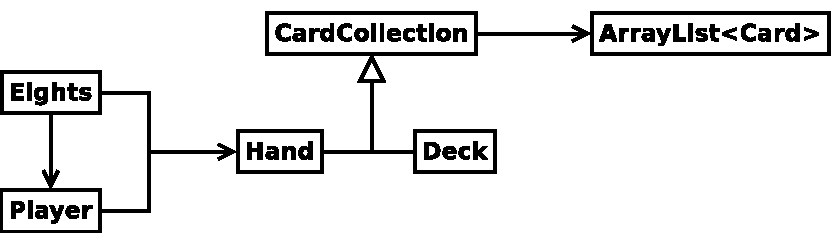
\includegraphics[width=0.9\textwidth]{figs/uml1.pdf}
\caption{UML diagram for the classes in this chapter.}
\label{fig.uml1}
\end{center}
\end{figure}

UML is an international standard, so almost any software engineer in the world could look at this diagram and understand our design.
And class diagrams are only one of many graphical representations defined in the UML standard.

We hope this final chapter has been a useful summary of all the techniques presented in the book, including variables, methods, conditionals, loops, arrays, objects, and algorithms.
Congratulations on making it to the end!


\section{Vocabulary}

\begin{description}

\term{collection}
An object that contains other objects, or more specifically, one of the objects in the Java library, like \java{ArrayList}, that contains objects.

\term{inheritance}
The ability to define a new class that has the same instance variables and methods of an existing class.

\term{subclass}
A class that inherits from, or extends, an existing class.

\term{superclass}
An existing class that is extended by another class.

%\term{override}
%To define a method in a subclass that replaces a method with the same name in a superclass.

\term{wrapper method}
A method that calls another method without doing much additional work.

\term{bottom-up development}
A way of developing programs by identifying simple pieces, implementing them, and then assembling them into more complex algorithms.

\term{HAS-A}
A relationship between two classes where one class ``has'' an instance of another class as one of its attributes.

\term{IS-A}
A relationship between two classes where one class extends another class; the subclass ``is'' an instance of the superclass.

\end{description}


\section{Exercises}

The code for this chapter is in the {\tt ch14} directory of {\tt ThinkJavaCode}.
See page~\pageref{code} for instructions on how to download the repository.
Before you start the exercises, we recommend that you compile and run the examples.

\begin{exercise}
Design a better strategy for the \java{Player.play} method.
For example, if there are multiple cards you can play, and one of them is an eight, you might want to play the eight.

\index{override}

Think of other ways you can minimize penalty points, such as playing the highest ranking cards first.
Write a new class that extends \java{Player} and overrides \java{play} to implement your strategy.
\end{exercise}


\begin{exercise}
Write a loop that plays the game 100 times and keeps track of how many times each player wins.
If you implemented multiple strategies in the previous exercise, you can play them against each other to evaluate which one works best.

{\it Hint:} Design a \java{Genius} class that extends \java{Player} and overrides the \java{play} method, and then replace one of the players with a \java{Genius} object.
\end{exercise}


\begin{exercise}
One limitation of the program we wrote in this chapter is that it only handles two players.
Modify the \java{Eights} class to create an \java{ArrayList} of players, and modify \java{nextPlayer} to select the next player.
\end{exercise}


\begin{exercise}
When we designed the program for this chapter, we tried to minimize the number of classes.
As a result, we ended up with a few awkward methods.
For example, \java{cardMatches} is a static method in \java{Player}, but it would be more natural if it were an instance method in \java{Card}.

The problem is that \java{Card} is supposed to be useful for any card game, not just {\it Crazy Eights}.
You can solve this problem by adding a new class, \java{EightsCard}, that extends \java{Card} and provides a method, \java{match}, that checks whether two cards match according to the rules of {\it Crazy Eights}.

At the same time, you could create a new class, \java{EightsHand}, that extends \java{Hand} and provides a method, \java{scoreHand}, that adds up the scores of the cards in the hand.
And while you're at it, you could add a method named \java{scoreCard} to \java{EightsCard}.

Whether or not you actually make these changes, draw a UML class diagram that shows this alternative object hierarchy.
\end{exercise}


\chapter{Arrays of Arrays}
\label{conway}

The last two chapters of this book use 2D graphics to illustrate more advanced object-oriented concepts.
If you haven't yet read Appendix~\ref{graphics}, you might want to read it now and get familiar with the \java{Canvas}, \java{Color}, and \java{Graphics} classes from the \java{java.awt} package.
In this chapter we use these classes to draw images and animations, and to run graphical simulations.


\section{Conway's Game of Life}

{\it The Game of Life}, or GoL for short, was developed by John Conway and popularized in 1970 in Martin Gardner's column in Scientific American.
Conway calls it a ``zero-player game'' because no players are needed to choose strategies or make decisions.
After you set up the initial conditions, you watch the game play itself.
That turns out to be more interesting than it sounds; you can read about it at \url{http://en.wikipedia.org/wiki/Conway's_Game_of_Life}.

\begin{figure}[!ht]
\begin{center}
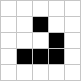
\includegraphics{figs/glider.png}
\caption{A ``Glider'' in the Game of Life.}
\label{fig:glider}
\end{center}
\end{figure}

The game board is a two-dimensional grid of square cells.
Each cell is either ``alive'' or ``dead''; the color of the cell indicates its status.
Figure~\ref{fig:glider} shows an example grid configuration.

\index{neighbor}

The game proceeds in time steps, during which each cell interacts with its neighbors in the eight adjacent cells.
At each step, the following rules are applied:

\begin{enumerate}
\small
\item A live cell with fewer than two live neighbors dies, as if by underpopulation.
\item A live cell with more than three live neighbors dies, as if by overpopulation.
\item A dead cell with exactly three live neighbors becomes a live cell, as if by reproduction.
\end{enumerate}

\index{stable configuration}

Notice some consequences of these rules.
If you start with a single live cell, it dies.
If all cells are dead, no cells come to life.
But if you have four cells in a square, they keep each other alive, so that's a ``stable'' configuration.

Another initial configuration is shown in Figure~\ref{fig:blinker}.
If you start with three horizontal cells, the center cell lives, the left and right cells die, and the top and bottom cells come to life.
The result after the first time step is three vertical cells.

During the next time step, the center cell lives, the top and bottom cells die, and the left and right cells come to life.
The result is three horizontal cells, so we're back where we started, and the cycle repeats forever.

\begin{figure}[!ht]
\begin{center}
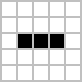
\includegraphics{figs/blinker-0.png}
\raisebox{38pt}{~$\longrightarrow$~}
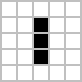
\includegraphics{figs/blinker-1.png}
\raisebox{38pt}{~$\longrightarrow$~}
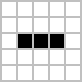
\includegraphics{figs/blinker-0.png}
\raisebox{38pt}{~$\longrightarrow$~ \ldots}
\caption{A ``Blinker'' in the Game of Life.}
\label{fig:blinker}
\end{center}
\end{figure}

Patterns like this are called ``periodic'', because they repeat after a period of two or more time steps.
But they are also considered stable, because the total number of live cells doesn't grow over time.

Most simple starting configurations either die out quickly or reach a stable configuration.
But there are a few starting conditions that display remarkable complexity.
One of those is the R-pentomino: it starts with only five cells, runs for 1103 time steps, and ends in a stable configuration with 116 live cells (see \url{http://www.conwaylife.com/wiki/R-pentomino}).

In the following sections, we'll implement the Game of Life in Java.
We'll first implement the cells, then the grid of cells, and finally the game itself.


\section{The Cell Class}

To represent the state of a cell, we use an integer, \java{state}, which is 0 for dead cells and 1 for live cells.
To represent the location, we use the \java{x} and \java{y} coordinates of the upper-left corner.
And to represent the size, we use an integer, \java{size}.

Here is a \java{Cell} class that declares these instance variables:

\begin{code}
public class Cell {
    private final int x;
    private final int y;
    private final int size;
    private int state;
}
\end{code}

Notice that \java{x}, \java{y}, and \java{size} are constants.
Once the cell is created, we don't want it to move or change size.
But \java{state} can and should change, so it is not a constant.

The next step is to write a constructor.
Here's one that takes \java{x}, \java{y}, and \java{size} as parameters, and sets {\tt state} to a default value.

\begin{code}
public Cell(int x, int y, int size) {
    this.x = x;
    this.y = y;
    this.size = size;
    this.state = 0;
}
\end{code}

%The following line uses the constructor to create a \java{Cell}.
%Its upper-left corner is at (0, 0), and the cell is 10x10 pixels.
%
%\begin{code}
%Cell cell = new Cell(0, 0, 10);
%\end{code}

The following method draws a cell.
Like the \java{paint} method in Appendix~\ref{graphics}, it takes a graphics context as a parameter.

\begin{code}
public static final Color[] COLORS = {Color.WHITE, Color.BLACK};

public void draw(Graphics g) {
    g.setColor(COLORS[this.state]);
    g.fillRect(x + 1, y + 1, size - 1, size - 1);
    g.setColor(Color.LIGHT_GRAY);
    g.drawRect(x, y, size, size);
}
\end{code}

The \java{draw} method uses the state of the cell to select a color from an array of \java{Color} objects.
Then it uses to \java{fillRect} to draw the center of the cell and \java{drawRect} to draw a light gray border.

We also need methods to get and set the cell's state.
We could just provide \java{getState} and \java{setState}, but the code will be more readable if we provide methods customized for the Game of Life:

\begin{code}
public boolean isOff() {
    return state == 0;
}

public boolean isOn() {
    return state == 1;
}
\end{code}

%\java{isOff} and \java{isOn} check the state of the cell.

\begin{code}
public void turnOff() {
    state = 0;
}

public void turnOn() {
    state = 1;
}
\end{code}

%\java{turnOff} and \java{turnOn} modify the state of the cell.


\section{Two-Dimensional Arrays}

\index{multidimensional array}

To represent a grid of cells, we can use a {\bf multidimensional array}.
To create a two-dimensional (2D) array, we specify the number of rows and columns:

\begin{code}
int rows = 4;
int cols = 3;
Cell[] array = new Cell[rows][cols];
\end{code}

The result is an array with 4 rows and 3 columns (representing a 3x4 grid).
Initially, the elements of the array are \java{null}.
We can fill the array with \java{Cell} objects like this:

\begin{code}
for (int r = 0; r < rows; r++) {
    int y = r * size;
    for (int c = 0; c < cols; c++) {
        int x = c * size;
        array[r][c] = new Cell(x, y, size);
    }
}
\end{code}

The loop variables \java{r} and \java{c} are the row and column indexes of the cells.
The variables \java{x} and \java{y} are the coordinates.
For example, if \java{size} is 10 pixels, the cell at index (1, 2) would be at coordinates (10, 20) on the screen.

In Java, a 2D array is really an array of arrays.
You can think of it as an array of rows, where each row is an array.
Figure~\ref{fig:2D-array} shows what it looks like.

\begin{figure}[!ht]
\begin{center}
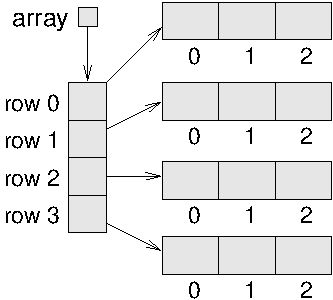
\includegraphics{figs/2D-array.pdf}
\caption{Storing rows and columns with a 2D array.}
\label{fig:2D-array}
\end{center}
\end{figure}

\index{row-major order}

%\java{array} is an array of references that refer to arrays of \java{Cell} objects.
When we write \java{array[r][c]}, Java uses the first index to select a row and the second index to select an element from the row.
This way of representing two-dimensional data is know as {\bf row-major order}.


\section{The GridCanvas Class}

Now that we have a \java{Cell} class and a way to represent a 2D array of cells, we can write a class to represent a grid of cells.
We encapsulate the code from the previous section and generalize it to construct a grid with any number of rows and columns:

\begin{code}
public class GridCanvas extends Canvas {
    private Cell[][] array;

    public GridCanvas(int rows, int cols, int size) {
        array = new Cell[rows][cols];
        for (int r = 0; r < rows; r++) {
            int y = r * size;
            for (int c = 0; c < cols; c++) {
                int x = c * size;
                array[r][c] = new Cell(x, y, size);
            }
        }

        // set the canvas size
        setSize(cols * size, rows * size);
    }
}
\end{code}

\index{IS-A}
\index{HAS-A}
\index{Graphics}

Using vocabulary from the previous chapter, \java{GridCanvas} ``is~a'' \java{Canvas} that ``has~a'' two-dimensional array of cells.
By extending the \java{Canvas} class from \java{java.awt}, we inherit methods for drawing graphics on the screen.

In fact, the code is surprisingly straightforward: to draw the grid, we simply draw each cell.
We use nested \java{for} loops to traverse the 2D array:

\begin{code}
public void draw(Graphics g) {
    for (Cell[] row : array) {
        for (Cell cell : row) {
            cell.draw(g);
        }
    }
}
\end{code}

The outer loop traverses the rows; the inner loop traverses the cells in each row.
You can almost read this method in English: ``For each \java{row} in the \java{array}, and for each \java{cell} in the \java{row}, draw the \java{cell} in the graphics context.''
Each cell contains its coordinates and size, so it knows how to draw itself.

Classes that extend \java{Canvas} are supposed to provide a method called \java{paint} that ``paints'' the contents of the \java{Canvas}.
It gets invoked when the \java{Canvas} is created and any time it needs to be redrawn, for example, when its window is moved or resized.

Here's the \java{paint} method for \java{GridCanvas}.
When the window management system calls \java{paint}, \java{paint} calls \java{draw}, which draws the cells.

\begin{code}
public void paint(Graphics g) {
    draw(g);
}
\end{code}


\section{Other grid methods}

In addition to \java{draw} and \java{paint}, the \java{Grid} class provides methods for working with the grid itself.
\java{numRows} and \java{numCols} return the number of rows and columns.
We can get this information from the 2D array, using \java{length}:

\begin{code}
public int numRows() {
    return array.length;
}

public int numCols() {
    return array[0].length;
}
\end{code}

Because we are using row-major order, the 2D array is an array of rows.
\java{numRows} simply returns the length of the rows array.
\java{numCols} returns the length of the first row, which is the number of columns.
Since the rows all have the same length, we only have to check one.

\java{GridCanvas} also provides a method that gets the \java{Cell} at a given location, and for convenience, a method that turns on the \java{Cell} at a given location.

\begin{code}
public Cell getCell(int r, int c) {
    return array[r][c];
}

public void turnOn(int r, int c) {
    array[r][c].turnOn();
}
\end{code}


\section{Starting the Game}
\label{conwaymain}

Now we're ready to implement the game.
To encapsulate the rules of GoL, we define a class named \java{Conway}.
The \java{Conway} class ``has~a'' \java{GridCanvas} that represents the state of the game.

This constructor makes a \java{GridCanvas} with 5 rows and 10 columns, with cells that are 20 pixels wide and high.
It then sets up the initial conditions.

\begin{code}
public class Conway {
    private GridCanvas grid;

    public Conway() {
        grid = new GridCanvas(5, 10, 20);
        grid.turnOn(2, 1);
        grid.turnOn(2, 2);
        grid.turnOn(2, 3);
        grid.turnOn(1, 7);
        grid.turnOn(2, 7);
        grid.turnOn(3, 7);
    }
}
\end{code}

\index{JFrame}

Before we implement the rest of the game, we'll write a \java{main} method that creates a \java{Conway} object and displays it.
We can use this method to test \java{Cell} and \java{GridCanvas}, and to develop the other methods we need.

\begin{code}
public static void main(String[] args) {
    String title = "Conway's Game of Life";
    Conway game = new Conway();
    JFrame frame = new JFrame(title);
    frame.setDefaultCloseOperation(JFrame.EXIT_ON_CLOSE);
    frame.setResizable(false);
    frame.add(game.grid);
    frame.pack();
    frame.setVisible(true);
    game.mainloop();
}
\end{code}

After constructing the \java{game} object, \java{main} instantiates a \java{JFrame}, which creates a window on the screen.
It then adds the \java{GridCanvas} inside the frame, resizes (``packs'') the frame to fit the canvas, and makes the frame visible.

Figure~\ref{fig:conway} shows the result.
The \java{JFrame} is configured to exit the program when closed.
Resizing the window is disabled.

\begin{figure}[!ht]
\begin{center}
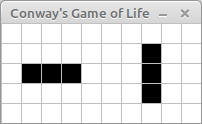
\includegraphics{figs/conway.png}
\caption{Screenshot of the initial \java{Conway} application.}
\label{fig:conway}
\end{center}
\end{figure}


\section{The Simulation Loop}
\label{mainloop}

At the end of \java{main}, we call \java{mainloop}, which uses a \java{while} loop to simulate the time steps of the Game of Life.
Here's a rough draft of this method:

\begin{code}
private void mainloop() {
    while (true) {
        this.update();
        grid.repaint();
        Thread.sleep(500);    // compiler error
    }
}
\end{code}

During each time step, we update the state of the game and repaint the \java{grid}.
We will present the \java{update} method in Section~\ref{sec:update}.

\java{repaint} comes from the \java{Canvas} class.
By default, it calls the \java{paint} method we provided, which calls \java{draw}.
The reason we use it here is that \java{repaint} does not require a \java{Graphics} object as a parameter.

\index{Thread.sleep}
\index{sleep}

\java{Thread.sleep(500)} causes the program to ``sleep'' for 500 milliseconds, or a half second.
Otherwise the program would run so fast we would not be able to see the animation.

\index{InterruptedException}
\index{Exception!Interrupted}

There's just one problem: compiling this code results in the error ``unreported exception InterruptedException''.
This message means we need to do some exception handling.


\section{Exception Handling}

So far, the only exceptions we have seen are run-time errors like ``array index out of bounds'' and ``null pointer''.
When one of these exceptions occur, Java displays a message and ends the program.

If you don't want the program to end, you can handle exceptions with a \java{try}-\java{catch} statement.
The syntax is similar to an \java{if}-\java{else} statement, and the logic is, too.
Here's what it looks like:

\index{try}
\index{catch}
\index{Statement!try}
\index{Statement!catch}

\begin{code}
try {
    Thread.sleep(500);
} catch (InterruptedException e) {
    // do nothing
}
\end{code}

First, Java runs the code in the try block, which calls \java{Thread.sleep} in this example.
If an \java{InterruptedException} occurs during the try block, Java executes the catch block.
In this example, the catch block contains a comment, so it doesn't do anything.

If a different exception occurs during the try block, Java does whatever it would do otherwise, which is probably to display a message and end the program.
If no exceptions occur during the try block, the catch block doesn't run and the program continues.

In this example, the effect of the \java{try}-\java{catch} statement is to ignore an ``interrupted'' exception if it occurs.

As an alternative, we could use the catch block to display a customized message, end the program, or handle the exception in whatever way is appropriate.
For example, if user input causes an exception, we could catch the exception and prompt the user to try again later.

There's more to learn about exception handling.
You can read about exceptions in the Java tutorials at \url{https://thinkjava.org/exceptions}.


\section{Counting neighbors}

\index{neighbor}

Now that you know about \java{try} and \java{catch}, we can use them to implement a useful method in \java{GridCanvas}.
Part of the GoL logic is to count the number of live neighbors.
Most cells have eight neighbors, as shown in Figure~\ref{fig:neighbors}.

\begin{figure}[!ht]
\begin{center}
\begin{tabular}{|p{1em}|p{1em}|p{1em}|p{1em}|p{1em}|}
\hline
  &   &   &   &   \\
\hline
  & 1 & 2 & 3 &   \\
\hline
  & 4 & * & 5 &   \\
\hline
  & 6 & 7 & 8 &   \\
\hline
  &   &   &   &   \\
\hline
\end{tabular}
\caption{Neighbors for a cell in the middle of the grid.}
\label{fig:neighbors}
\end{center}
\end{figure}

However, cells on the edges and in the corners have fewer neighbors.
If we try to count all possible neighbors, we'll go out of bounds.
%(Normally in the Game of Life, we don't have this problem because the grid size is infinite.
%But we thought that version might be a bit much for this chapter!)
The following method uses a \java{try}-\java{catch} statement to deal with these special cases.

\begin{code}
public int test(int r, int c) {
    try {
        if (array[r][c].isOn()) {
            return 1;
        }
    } catch (ArrayIndexOutOfBoundsException e) {
        // cell doesn't exist
    }
    return 0;
}
\end{code}

The \java{test} method takes a row index, \java{r}, and a column index, \java{c}.
It tries to look up the \java{Cell} at that location.
If both of the indexes are in bounds, the \java{Cell} exists.
In that case, \java{test} returns 1 if the \java{Cell} is on and 0 otherwise.

If either of the indexes is out of bounds, the array lookup throws an exception, but the catch clause catches and ignores it.
Then \java{test} resumes and returns 0.
So the non-existent cells around the perimeter are considered to be off.

Now we can use \java{test} to implement \java{countAlive}, which takes a grid location, \java{(r, c)}, and returns the number of live neighbors surrounding that location.

\begin{code}
private int countAlive(int r, int c) {
    int count = 0;
    count += grid.test(r - 1, c - 1);
    count += grid.test(r - 1, c);
    count += grid.test(r - 1, c + 1);
    count += grid.test(r, c - 1);
    count += grid.test(r, c + 1);
    count += grid.test(r + 1, c - 1);
    count += grid.test(r + 1, c);
    count += grid.test(r + 1, c + 1);
    return count;
}
\end{code}

Because \java{test} handles ``out of bounds'' exceptions, this method works for any values of \java{r} and \java{c}.


\section{Updating the grid}
\label{sec:update}

Now we are ready to write \java{update}, which gets invoked each time through the simulation loop.
It uses the GoL rules to compute the state of the grid after the next time step.

\begin{code}
public void update() {
    int[][] counts = countNeighbors();
    updateGrid(counts);
}
\end{code}

The rules of GoL specify that you have to update the cells ``simultaneously''; that is, you have to count the neighbors for all cells before you can update any of them.

We do that by traversing the grid twice: first, \java{countNeighbors} counts the live neighbors for each cell and puts the results in an array named \java{counts}; second, \java{updateGrid} updates the cells.
Here's \java{countNeighbors}:

\begin{code}
private int[][] countNeighbors() {
    int rows = grid.numRows();
    int cols = grid.numCols();

    int[][] counts = new int[rows][cols];
    for (int r = 0; r < rows; r++) {
        for (int c = 0; c < cols; c++) {
            counts[r][c] = countAlive(r, c);
        }
    }
    return counts;
}
\end{code}

\java{countNeighbors} traverses the cells in the grid and uses \java{countAlive} from the previous section to count the neighbors.
The return value is a 2D array of integers with the same size as \java{grid}.

In contrast to the \java{draw} method of \java{GridCanvas}, which uses enhanced \java{for} loops, \java{countNeighbors} uses standard \java{for} loops.
The reason is that, in this example, we need the indexes \java{r} and \java{c} to store the neighbor counts.

\java{updateGrid} uses \java{getCell} to select each \java{Cell} in the grid and \java{updateCell} to do the update.

\begin{code}
private void updateGrid(int[][] counts) {
    int rows = grid.numRows();
    int cols = grid.numCols();

    for (int r = 0; r < rows; r++) {
        for (int c = 0; c < cols; c++) {
            Cell cell = grid.getCell(r, c);
            updateCell(cell, counts[r][c]);
        }
    }
}
\end{code}

\java{updateCell} implements the GoL rules: if the cell is alive, it dies if it has fewer than 2 or more than 3 neighbors; if the cell is dead, it comes to life if it has exactly 3.

\begin{code}
private static void updateCell(Cell cell, int count) {
    if (cell.isOn()) {
        if (count < 2 || count > 3) {
            cell.turnOff();
        }
    } else {
        if (count == 3) {
            cell.turnOn();
        }
    }
}
\end{code}

The \java{updateCell} method \java{private}, because it is a helper method not intended to be invoked from outside the class.
It's also \java{static}, because it does not depend on \java{grid}.

Now our implementation of the Game of Life is complete.
We think it's is pretty fun, and we hope you agree.
But more importantly, this example is meant to demonstrate the use of 2D arrays and an object-oriented design that's a little more substantial than previous chapters.

%In the exercises at the end of this chapter, you'll have a chance to run the code, test other initial conditions, and explore other games with similar rules.


\section{Vocabulary}

\begin{description}

\term{multidimensional array}
An array with more than one dimension; also known as an ``array of arrays''.

\term{row-major order}
Storing data in a two-dimensional array first by rows and then by columns.

\end{description}


\section{Exercises}

The code for this chapter is in the {\tt ch15} directory of {\tt ThinkJavaCode2}.
See page~\pageref{code} for instructions on how to download the repository.
Before you start the exercises, we recommend that you compile and run the examples.


\begin{exercise}
In \java{GridCanvas}, write a method named \java{countOn} that returns the total number of cells that are ``on''.
This method can be used, for example, to track the population in Game of Life over time.
\end{exercise}


\begin{exercise}
In our version of the Game of Life, the grid has a finite size.
As a result, moving objects such as gliders either crash into the wall or go out of bounds.

An interesting variation of the Game of Life is a ``toroidal'' grid, meaning that the cells ``wrap around'' on the edges.
Modify the \java{test} method of \java{GridCanvas} so that the coordinates \java{r} and \java{c} map to the opposite side of the grid if they are too low or two high.

Run your code with a Glider (see Figure~\ref{fig:glider}) to see if it works.
You can initialize the Glider by modifying the constructor in the \java{Conway} class, or by reading it from a file (see the next exercise).
\end{exercise}


%CSM idea for another exercise: 2D arrays -- grow/shrink the grid
%ABD: Good idea, but I think we have enough for now.

%\begin{exercise}
%Another way to handle edge collisions is to expand the grid as needed.
%\end{exercise}


\begin{exercise}

% TODO: Remove the solution from the starter code.

The ``LifeWiki'' \url{http://conwaylife.com/wiki/} has a fascinating collection of patterns for the Game of Life.
These patterns are stored in a file format that is easy to read, in files with the suffix ``\verb|.cells|''.

For example, here is an 8x10 grid with a glider near the upper-left corner:

\begin{stdout}
!Name: Glider
..........
..O.......
...O......
.OOO......
..........
..........
..........
..........
\end{stdout}

Lines that begin with \java{!} are comments and should be ignored.
The rest of the file describes the grid, row by row.
A period represents a dead cell, and an uppercase O represents a live cell.
See \url{http://conwaylife.com/wiki/Plaintext} for more examples.

\begin{enumerate}

\item Create a plain text file with the contents shown above, and save the file as \verb|glider.cells| in the same directory as your code.

% ABD: Should this be a constructor?  I would make it a static method that builds and returns a Conway object, on the principle that constructors generally take parameters that line up with the instance variables, and methods that do substantial work should not be constructors.  But that might be a Pythonic principle that isn't Javai-idiomatic.

\item Define a constructor for the \java{Conway} class that takes a string representing the name (or path) of a ``.cells'' file.
Here is a starting point:

\begin{code}
public Conway(String path) {
    File file = new File(path);
    Scanner scan = new Scanner(file);
}
\end{code}

\item Modify the main method to invoke the constructor as follows:

\begin{code}
Conway game = new Conway("glider.cells");
\end{code}

\item Handle the \java{FileNotFoundException} that may be thrown when creating a \java{Scanner} for a \java{File} by invoking \java{printStackTrace} on the exception object and calling \java{System.exit()} with a status of 1, indicating an error.

\item Continue implementing the constructor by reading all non-comment lines into an \java{ArrayList} using \java{hasNextLine} and \java{nextLine} of the \java{Scanner}.

\item Determine the number of rows and columns of the grid by examining the \java{ArrayList} contents.

\item Create and initialize a \java{GridCanvas} based on the \java{ArrayList}.

\end{enumerate}

Once your constructor is working, you will be able to run many of the patterns on the LifeWiki.
You might want to add a margin of empty cells around the initial pattern, to give it room to grow.

\end{exercise}


\begin{exercise}
Some files on the LifeWiki use ``Run Length Encoding'' (RLE) instead of plain text.
The basic idea of RLE is to describe the number of dead and alive cells, rather than type out each individual cell.

For example, \verb|glider.cells| from the previous exercise could be represented this way with RLE:

\begin{stdout}
#C Name: Glider
x = 10, y = 8
$2bo$3bo$b3o!
\end{stdout}%$

The first line specifies \verb|x| (the number of columns) and \verb|y| (the number of rows).
Subsequent lines consist of the letters \verb|b| (dead), \verb|o| (alive), and \verb|$| (end of line), optionally preceded by a count.
The pattern ends with \verb|!|, after which any remaining file contents are ignored.

Lines beginning with \java{#} have special meaning and are not part of the pattern.
For example, \java{#C} is a comment line.
You can read more about RLE format on \url{http://conwaylife.com/wiki/RLE}.

\begin{enumerate}

\item Create a plain text file with the contents shown above, and save the file as \verb|glider.rle| in the same directory as your code.

%ABD: As in the previous exercise, should this be a constructor?  And either way, should it be a separate method, or modify the other method to read both formats?

\item Modify your constructor from the previous exercise to check the last three characters of the \java{path}.
If they are \java{"rle"}, then you will need to process the file as RLE.
Otherwise, assume the file is in ``.cells'' format.

\item In the end, your constructor should be able to read and initialize grids in both formats.
Test your constructor by modifying the \java{main} method to read different files.

\end{enumerate}

\end{exercise}

\begin{exercise}

Now that we've finished the Game of Life, we can use the \java{Cell} and \java{GridCanvas} classes to implement other simulations.
One of the most interesting zero-player games is {\it Langton's Ant}, which models an ``ant'' that walks around a grid of cells.
The ant follows only two simple rules:

\begin{enumerate}
\item If the ant is on a white cell, it turns to the right, makes the cell black, and moves forward.
\item If the ant is on a black cell, it turns to the left, makes the cell white, and moves forward.
\end{enumerate}

Because the rules are simple, you might expect the ant to do something simple, like make a square or repeat a simple pattern.
But starting on a grid with all white cells, the ant makes more than 10,000 steps in a seemingly random pattern before it settles into a repeating loop of 104 steps.
You can read more about it at \url{http://en.wikipedia.org/wiki/Langton's_ant}.

Reusing the classes we developed in this chapter, write an implementation of Langton's Ant.

\end{exercise}



\chapter{Abstract Classes}

In the previous chapter, we developed classes to implement Conway's Game of Life.
As an exercise, you had a chance to implement Langton's Ant.

In this chapter, we present a solution to that exercise and use it to demonstrate a new Java feature, ``abstract classes''.


\section{Langton's Ant Solution}

We begin by defining a \java{Langton} class that ``has~a'' grid and information about the ant.
The constructor takes the grid dimensions as parameters.

\begin{code}
public class Langton {
    private GridCanvas grid;
    private int xpos;
    private int ypos;
    private int head; // 0=North, 1=East, 2=South, 3=West

    public Langton(int rows, int cols) {
        grid = new GridCanvas(rows, cols, 10);
        xpos = rows / 2;
        ypos = cols / 2;
        head = 0;
    }
}
\end{code}

\java{grid} is a \java{GridCanvas} object, which represents the state of the cells.
\java{xpos} and \java{ypos} are the coordinates of the ant, and \java{head} is the ``heading'' of the ant, that is, what direction it is facing.
\java{head} is an integer with four possible values, where 0 means the ant is facing ``north'', that is, toward the top of the screen, 1 means ``east'', etc.

Here's the \java{update} method that implements the rules for Langton's ant:

\begin{code}
public void update() {
    flipCell();
    moveAnt();
}
\end{code}

The \java{flipCell} method gets the \java{Cell} at the ant's location, figures out which way to turn, and changes the state of the cell.

\begin{code}
private void flipCell() {
    Cell cell = grid.getCell(xpos, ypos);
    if (cell.isOff()) {
        // at a white square; turn right and flip color
        head = (head + 1) % 4;
        cell.turnOn();
    } else {
        // at a black square; turn left and flip color
        head = (head + 3) % 4;
        cell.turnOff();
    }
}
\end{code}

We use the remainder operator, \verb"%", to make \java{head} wrap around: if \java{head} is 3 and we turn right, it wraps around to 0; if \java{head} is 0 and we turn left, it wraps around to 3.

The \java{moveAnt} method moves the ant forward one square, using \java{head} to determine which way is forward.

\begin{code}
private void moveAnt() {
    if (head == 0) {
        ypos -= 1;
    } else if (head == 1) {
        xpos += 1;
    } else if (head == 2) {
        ypos += 1;
    } else {
        xpos -= 1;
    }
}
\end{code}

If you run this code with a grid size of 61x61 or larger, you will see the ant eventually settle into a repeating pattern.

Here is the \java{main} method we use to create and display the \java{Langton} object:

\begin{code}
public static void main(String[] args) {
    String title = "Langton's Ant";
    Langton game = new Langton(61, 61);
    JFrame frame = new JFrame(title);
    frame.setDefaultCloseOperation(JFrame.EXIT_ON_CLOSE);
    frame.setResizable(false);
    frame.add(game.grid);
    frame.pack();
    frame.setVisible(true);
    game.mainloop();
}
\end{code}

Most of this method is the same as the \java{main} we used to create and run \java{Conway}, in Section~\ref{conwaymain}.
It creates and configures a \java{JFrame} and runs \java{mainloop}.


\section{Refactoring}

Whenever you see repeated code like \java{main}, you should think about ways to remove it.
In the Chapter~\ref{eights}, we used inheritance to eliminate repeated code.
We'll do something similar with \java{Conway} and \java{Langton}.

First, we define a superclass named \java{Automaton} where we will put the code that \java{Conway} and \java{Langton} have in common.

\begin{code}
public class Automaton {
    private GridCanvas grid;

    public void run(String title, int rate) {
        JFrame frame = new JFrame(title);
        frame.setDefaultCloseOperation(JFrame.EXIT_ON_CLOSE);
        frame.setResizable(false);
        frame.add(this.grid);
        frame.pack();
        frame.setVisible(true);
        this.mainloop(rate);
    }
}
\end{code}

\java{Automaton} declares \java{grid} as an instance variable, so every \java{Automaton} ``has~a'' \java{GridCanvas}.
It also provides \java{run}, which contains the code that creates and configures the \java{JFrame}.

The \java{run} method takes two parameters: the window \java{title} and the frame \java{rate}, that is, the number of time steps to show per second.
It uses \java{title} when creating the \java{JFrame}, and it passes \java{rate} to \java{mainloop}:

\begin{code}
private void mainloop(int rate) {
    while (true) {

        // update the drawing
        this.update();
        grid.repaint();

        // delay the simulation
        try {
            Thread.sleep(1000 / rate);
        } catch (InterruptedException e) {
            // do nothing
        }
    }
}
\end{code}

\java{mainloop} contains the code we first saw in Section~\ref{mainloop}.
It runs a \java{while} loop forever (or until the window closes).
Each time through the loop, it runs \java{update} to update \java{grid} and then \java{repaint} to redraw the grid.

Then it calls \java{Thread.sleep} with a delay that depends on \java{rate}.
For example, if {\tt rate} is 2, we should draw two frames per second, so the delay is a half second, or 500 milliseconds.

\index{refactoring}

This process of reorganizing existing code, without changing its behavior, is known as {\bf refactoring}.
We're almost finished; we just need to redesign \java{Conway} and \java{Langton} to extend \java{Automaton}.


\section{Abstract Classes}

So far the implementation works, and if we are not planning to implement any other zero-person games, we could leave well enough alone.
But there are a few problems with the current design:

\begin{enumerate}

\item The \java{grid} attribute is \java{private}, making it inaccessible in \java{Conway} and \java{Langton}.
We could make it \java{public}, but then other (unrelated) classes would have access to it as well.

\item The \java{Automaton} class has no constructors, and even if it did, there would be no reason to create an instance of this class.

\item The \java{Automaton} class does not provide an implementation of \java{update}.
In order to work properly, subclasses need to provide one.

\end{enumerate}

\index{protected}
\index{abstract}

Java provides language features to solve these problems:

\begin{enumerate}

\item We can make the \java{grid} attribute \java{protected}, which means it's accessible to subclasses but not other classes.

\item We can make the class \java{abstract}, which means it cannot be instantiated.
If you attempt to create an object for an abstract class, you will get a compiler error.

\item We can declare \java{update} as an \java{abstract} method, meaning that it must be overriden in subclasses.
If the subclass does not override an abstract method, you will get a compiler error.
\end{enumerate}

Here's what \java{Automaton} looks like as an abstract class:

\begin{code}
public abstract class Automaton {
    protected GridCanvas grid;

    public abstract void update();

    public void run(String title, int delay) {
        // body of this method omitted
    }

    private void mainloop(int rate) {
        // body of this method omitted
    }
}
\end{code}

Notice that the \java{update} method has no body.
The declaration specifies the name, arguments, and return type.
But it does not provide an implementation, because it is an abstract method.

Notice also the word \java{abstract} on the first line, which declares that \java{Automaton} is an abstract class.
In order to have any abstract methods, a class must be declared as abstract.

Any class that extends \java{Automaton} must provide an implementation of \java{update}; the declaration here allows the compiler to check.

Here's what \java{Conway} looks like as a subclass of \java{Automaton}:

\begin{code}
public class Conway extends Automaton {

    // same methods as before, except mainloop is removed

    public static void main(String[] args) {
        String title = "Conway's Game of Life";
        Conway game = new Conway("pulsar.cells", 2);
        game.run(title, 2);
    }
}
\end{code}

\java{Conway} extends \java{Automaton}, so it inherits the instance variable \java{grid} and the methods \java{run} and \java{mainloop}.
But because \java{Automaton} is abstract, \java{Conway} has to provide \java{update} and a constructor (which it has already).

Abstract classes are essentially ``incomplete'' class definitions that specify methods to be implemented by subclasses.
But they also provide attributes and methods to be inherited, thus eliminating repeated code.


\section{Vocabulary}

\begin{description}

\term{refactor}
The process of restructuring or reorganizing existing code without changing its behavior.

\term{abstract class}
A class that is declared as \java{abstract}; it cannot be instantiated, and it may (or may not) include abstract methods.

\term{concrete class}
A class that is \emph{not} declared as \java{abstract}; each of its methods must have an implementation.

\end{description}


\section{Exercises}

\begin{exercise}

The last section of this chapter introduces \java{Automaton} as an abstract class and rewrites \java{Conway} as a subclass of \java{Automaton}.
Now it's your turn.
Rewrite \java{Langton} as a subclass of \java{Automaton}, removing the code that's no longer needed.

\end{exercise}


\begin{exercise}

Mathematically speaking, Game of Life and Langton's Ant are cellular automata, where ``cellular'' means it has cells, and ``automaton'' means it runs itself.
See \url{https://en.wikipedia.org/wiki/Cellular_automaton} for more discussion.

Implement another cellular automaton of your choice.
You may have to modify \java{Cell} and/or \java{GridCanvas}, in addition to extending \java{Automaton}.
For example, Brian's Brain (\url{https://en.wikipedia.org/wiki/Brian's_Brain}) requires three states: ``on'', ``dying'', and ``off''.

\end{exercise}


\chapter{Reusing Classes}

In Chapter~\ref{conway}, we developed classes to implement Conway's Game of Life.
%As an exercise, you had a chance to implement Langton's Ant.
We can reuse the \java{Cell} and \java{GridCanvas} classes to implement other simulations.
One of the most interesting zero-player games is {\it Langton's Ant}, which models an ``ant'' that walks around a grid.
The ant follows only two simple rules:

\begin{enumerate}
\item If the ant is on a white cell, it turns to the right, makes the cell black, and moves forward.
\item If the ant is on a black cell, it turns to the left, makes the cell white, and moves forward.
\end{enumerate}

Because the rules are simple, you might expect the ant to do something simple, like make a square or repeat a simple pattern.
But starting on a grid with all white cells, the ant makes more than 10,000 steps in a seemingly random pattern before it settles into a repeating loop of 104 steps.
You can read more about it at \url{https://en.wikipedia.org/wiki/Langton's_ant}.

%Reusing the classes we developed in this chapter, write an implementation of Langton's Ant.
%We present a solution to this exercise in Appendix~\ref{app:langton}.

In this chapter, we present a solution to Langton's Ant and use it to demonstrate more advanced object-oriented techniques.


\section{Langton's Ant}

We begin by defining a \java{Langton} class that has a grid and information about the ant.
The constructor takes the grid dimensions as parameters.

\begin{code}
public class Langton {
    private GridCanvas grid;
    private int xpos;
    private int ypos;
    private int head; // 0=North, 1=East, 2=South, 3=West

    public Langton(int rows, int cols) {
        grid = new GridCanvas(rows, cols, 10);
        xpos = rows / 2;
        ypos = cols / 2;
        head = 0;
    }
}
\end{code}

\java{grid} is a \java{GridCanvas} object, which represents the state of the cells.
\java{xpos} and \java{ypos} are the coordinates of the ant, and \java{head} is the ``heading'' of the ant, that is, what direction it is facing.
\java{head} is an integer with four possible values, where 0 means the ant is facing ``north'', that is, toward the top of the screen, 1 means ``east'', etc.

Here's an \java{update} method that implements the rules for Langton's ant:

\begin{code}
public void update() {
    flipCell();
    moveAnt();
}
\end{code}

The \java{flipCell} method gets the \java{Cell} at the ant's location, figures out which way to turn, and changes the state of the cell.

\begin{code}
private void flipCell() {
    Cell cell = grid.getCell(xpos, ypos);
    if (cell.isOff()) {
        head = (head + 1) % 4;    // turn right
        cell.turnOn();
    } else {
        head = (head + 3) % 4;    // turn left
        cell.turnOff();
    }
}
\end{code}

We use the remainder operator, \verb"%", to make \java{head} wrap around: if \java{head} is 3 and we turn right, it wraps around to 0; if \java{head} is 0 and we turn left, it wraps around to 3.

Notice that to turn right, we add 1 to \java{head}.
To turn left, we could subtract 1, but \verb"-1 % 4" is \verb"-1" in Java.
So we add 3 instead, since one left turn is the same as three right turns.

The \java{moveAnt} method moves the ant forward one square, using \java{head} to determine which way is forward.

\begin{code}
private void moveAnt() {
    if (head == 0) {
        ypos -= 1;
    } else if (head == 1) {
        xpos += 1;
    } else if (head == 2) {
        ypos += 1;
    } else {
        xpos -= 1;
    }
}
\end{code}

Here is the \java{main} method we use to create and display the \java{Langton} object:

\begin{code}
public static void main(String[] args) {
    String title = "Langton's Ant";
    Langton game = new Langton(61, 61);
    JFrame frame = new JFrame(title);
    frame.setDefaultCloseOperation(JFrame.EXIT_ON_CLOSE);
    frame.setResizable(false);
    frame.add(game.grid);
    frame.pack();
    frame.setVisible(true);
    game.mainloop();
}
\end{code}

Most of this code is the same as the \java{main} we used to create and run \java{Conway}, in Section~\ref{conwaymain}.
It creates and configures a \java{JFrame} and runs \java{mainloop}.

And that's everything!
If you run this code with a grid size of \mbox{61 x 61} or larger, you will see the ant eventually settle into a repeating pattern.

Because we designed \java{Cell} and \java{GridCanvas} to be reusable, we didn't have to modify them at all.
However, we now have two copies of the \java{main} method---one on \java{Conway}, and one in \java{Langton}.


\section{Refactoring}

Whenever you see repeated code like \java{main}, you should think about ways to remove it.
In the Chapter~\ref{eights}, we used inheritance to eliminate repeated code.
We'll do something similar with \java{Conway} and \java{Langton}.

First, we define a superclass named \java{Automaton} where we will put the code that \java{Conway} and \java{Langton} have in common.

\begin{code}
public class Automaton {
    private GridCanvas grid;

    public void run(String title, int rate) {
        JFrame frame = new JFrame(title);
        frame.setDefaultCloseOperation(JFrame.EXIT_ON_CLOSE);
        frame.setResizable(false);
        frame.add(this.grid);
        frame.pack();
        frame.setVisible(true);
        this.mainloop(rate);
    }
}
\end{code}

\java{Automaton} declares \java{grid} as an instance variable, so every \java{Automaton} ``has~a'' \java{GridCanvas}.
It also provides \java{run}, which contains the code that creates and configures the \java{JFrame}.

The \java{run} method takes two parameters: the window \java{title} and the frame \java{rate}, that is, the number of time steps to show per second.
It uses \java{title} when creating the \java{JFrame}, and it passes \java{rate} to \java{mainloop}:

\begin{code}
private void mainloop(int rate) {
    while (true) {

        // update the drawing
        this.update();
        grid.repaint();

        // delay the simulation
        try {
            Thread.sleep(1000 / rate);
        } catch (InterruptedException e) {
            // do nothing
        }
    }
}
\end{code}

\java{mainloop} contains the code we first saw in Section~\ref{mainloop}.
It runs a \java{while} loop forever (or until the window closes).
Each time through the loop, it runs \java{update} to update \java{grid} and then \java{repaint} to redraw the grid.

Then it calls \java{Thread.sleep} with a delay that depends on \java{rate}.
For example, if {\tt rate} is 2, we should draw two frames per second, so the delay is a half second, or 500 milliseconds.

\index{refactoring}

This process of reorganizing existing code, without changing its behavior, is known as {\bf refactoring}.
We're almost finished; we just need to redesign \java{Conway} and \java{Langton} to extend \java{Automaton}.


\section{Abstract Classes}

So far the implementation works, and if we are not planning to implement any other zero-person games, we could leave well enough alone.
But there are a few problems with the current design:

\begin{enumerate}

\item The \java{grid} attribute is \java{private}, making it inaccessible in \java{Conway} and \java{Langton}.
We could make it \java{public}, but then other (unrelated) classes would have access to it as well.

\item The \java{Automaton} class has no constructors, and even if it did, there would be no reason to create an instance of this class.

\item The \java{Automaton} class does not provide an implementation of \java{update}.
In order to work properly, subclasses need to provide one.

\end{enumerate}

\index{protected}
\index{abstract}

Java provides language features to solve these problems:

\begin{enumerate}

\item We can make the \java{grid} attribute \java{protected}, which means it's accessible to subclasses but not other classes.

\item We can make the class \java{abstract}, which means it cannot be instantiated.
If you attempt to create an object for an abstract class, you will get a compiler error.

\item We can declare \java{update} as an \java{abstract} method, meaning that it must be overridden in subclasses.
If the subclass does not override an abstract method, you will get a compiler error.
\end{enumerate}

Here's what \java{Automaton} looks like as an abstract class:

\begin{code}
public abstract class Automaton {
    protected GridCanvas grid;

    public abstract void update();

    public void run(String title, int delay) {
        // body of this method omitted
    }

    private void mainloop(int rate) {
        // body of this method omitted
    }
}
\end{code}

Notice that the \java{update} method has no body.
The declaration specifies the name, arguments, and return type.
But it does not provide an implementation, because it is an abstract method.

Notice also the word \java{abstract} on the first line, which declares that \java{Automaton} is an abstract class.
In order to have any abstract methods, a class must be declared as abstract.

Any class that extends \java{Automaton} must provide an implementation of \java{update}; the declaration here allows the compiler to check.

Here's what \java{Conway} looks like as a subclass of \java{Automaton}:

\begin{code}
public class Conway extends Automaton {

    // same methods as before, except mainloop is removed

    public static void main(String[] args) {
        String title = "Conway's Game of Life";
        Conway game = new Conway("pulsar.cells", 2);
        game.run(title, 2);
    }
}
\end{code}

\java{Conway} extends \java{Automaton}, so it inherits the \java{protected} instance variable \java{grid} and the methods \java{run} and \java{mainloop}.
But because \java{Automaton} is abstract, \java{Conway} has to provide \java{update} and a constructor (which it has already).

Abstract classes are essentially ``incomplete'' class definitions that specify methods to be implemented by subclasses.
But they also provide attributes and methods to be inherited, thus eliminating repeated code.


\section{UML Diagram}

At the beginning of the chapter, with had three classes: \java{Cell}, \java{GridCanvas}, and \java{Conway}.
We then developed \java{Langton}, which had almost the same \java{main} method as \java{Conway}.
So we refactored the code and created \java{Automaton}.
Figure~\ref{fig:uml2} summarizes the final design.

\begin{figure}[!ht]
\begin{center}
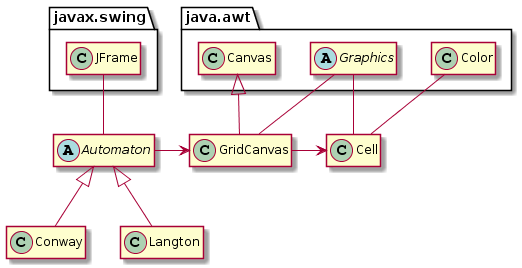
\includegraphics[width=0.75\textwidth]{figs/uml2.png}
\caption{UML class diagram of \java{Conway} and \java{Langton} applications.}
\label{fig:uml2}
\end{center}
\end{figure}

\index{IS-A}
\index{HAS-A}

The diagram shows three examples of inheritance: \java{Conway} is an \java{Automaton}, \java{Langton} is an \java{Automaton}, and \java{GridCanvas} is a Canvas.
It also shows two examples of composition: \java{Automaton} has a \java{GridCanvas}, and \java{GridCanvas} has a 2D array of \java{Cell}s.

The diagram also shows that \java{Automaton} uses \java{JFrame}, \java{GridCanvas} uses \java{Graphics}, and \java{Cell} uses \java{Graphics} and \java{Color}.

\java{Automaton} is in italics to indicate that it is an abstract class.
As it happens, \java{Graphics} is an abstract class, too.

%According to the documentation, its design ``allows an application to draw onto components that are realized on various devices, as well as onto off-screen images.''
%That's the beauty of abstraction; our code works regardless how and where it's drawn.

One of the challenges of object-oriented programming is keeping track of a large number of classes and the relationships between them.
UML class diagrams can help.


\section{Vocabulary}

\begin{description}

\term{refactor}
The process of restructuring or reorganizing existing code without changing its behavior.

\term{abstract class}
A class that is declared as \java{abstract}; it cannot be instantiated, and it may (or may not) include abstract methods.

\term{concrete class}
A class that is {\em not} declared as \java{abstract}; each of its methods must have an implementation.

\end{description}


\section{Exercises}

The code for this chapter is in the {\it ch16} directory of {\it ThinkJavaCode2}.
See page~\pageref{code} for instructions on how to download the repository.
Before you start the exercises, we recommend that you compile and run the examples.

\begin{exercise}

The last section of this chapter introduced \java{Automaton} as an abstract class and rewrote \java{Conway} as a subclass of \java{Automaton}.
Now it's your turn: rewrite \java{Langton} as a subclass of \java{Automaton}, removing the code that's no longer needed.

\end{exercise}


\begin{exercise}

Mathematically speaking, Game of Life and Langton's Ant are cellular automata, where ``cellular'' means it has cells, and ``automaton'' means it runs itself.
See \url{https://en.wikipedia.org/wiki/Cellular_automaton} for more discussion.

Implement another cellular automaton of your choice.
You may have to modify \java{Cell} and/or \java{GridCanvas}, in addition to extending \java{Automaton}.
For example, Brian's Brain (\url{https://en.wikipedia.org/wiki/Brian's_Brain}) requires three states: ``on'', ``dying'', and ``off''.

\end{exercise}


\appendix
%\addtocontents{toc}{\protect\newpage}

%~ \part{Appendixes}

%BEGIN LATEX
\renewcommand{\chaptermark}[1]{\markboth{Appendix \thechapter ~~ #1}{}}
%END LATEX

\chapter{Tools}
\label{tools}

\index{IDE}

The steps for compiling, running, and debugging Java code depend on your development environment and operating system.
We avoided putting these details in the main text, because they can be distracting.
Instead, we provide this appendix with a brief introduction to DrJava---an {\bf integrated development environment} (IDE) that is helpful for beginners---and other development tools, including Checkstyle for code quality and JUnit for testing.


\section{Installing DrJava}
\label{drjava}

The easiest way to start programming in Java is to use a website that compiles and runs Java code in the browser.
Examples include \url{https://repl.it/}, \url{https://trinket.io/}, \url{https://jdoodle.com/}, and others.

If you are unable to install software on your computer (which is often the case in public schools and Internet caf\'{e}s), you can use these online development environments for almost everything in this book.

But if you want to compile and run Java programs on your own computer, you will need:

\begin{itemize}

\item The {\bf Java Development Kit} (JDK), which includes the compiler, the {\bf Java Virtual Machine} (JVM) that interprets the compiled byte code, and other tools such as Javadoc.

\index{JDK}
\index{JVM}
\index{virtual machine}
\index{Javadoc}

\index{text editor}
\index{DrJava}

\item A {\bf text editor} such as Atom, Notepad++, or Sublime Text, and/or an IDE such as DrJava, Eclipse, jGrasp, or NetBeans.

\end{itemize}

The JDK we recommend is OpenJDK, an open-source implementation of Java~SE (Standard Edition).
The IDE we recommend is DrJava, which is an open-source development environment written in Java (see Figure~\ref{fig.drjava1}).

To install OpenJDK, visit \url{https://adoptopenjdk.net}.
Download and run the installer for your operating system.

%To install the JDK, search the web for ``download JDK'' which should take you to Oracle's website.
%Scroll down to ``Java Platform, Standard Edition'' and click the download button under JDK.
%Then accept the license agreement and select the installer for your operating system.
%Don't forget to run the installer after you download it!

\index{JAR}

% TODO: ML suggest pointing to an installation video (or making one)

To install DrJava, visit \url{http://drjava.org/} and download the {\bf JAR} file.
We recommend that you save it to your Desktop or another convenient location.
Simply double-click the JAR file to run DrJava.
Refer to the DrJava documentation (\url{http://drjava.org/docs/quickstart/}) for more details.

\begin{figure}[!ht]
\begin{center}
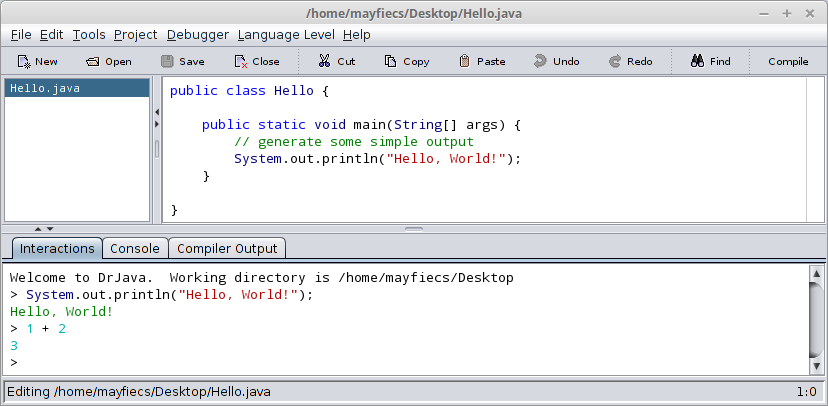
\includegraphics[width=0.95\textwidth]{figs/drjava-hello.png}
\caption{Screenshot of DrJava editing the Hello World program.}
\label{fig.drjava1}
\end{center}
\end{figure}

When running DrJava for the first time, we recommend you change three settings from the {\sf Edit $>$ Preferences} menu under {\sf Miscellaneous}: set the {\sf Indent Level} to 4, check the {\sf Automatically Close Block Comments} box, and uncheck the {\sf Keep Emacs-style Backup Files} box.

%We will use DrJava as the primary development environment throughout this book.

%Step-by-step instructions for installing the JDK and configuring DrJava are available on this book's website: \url{https://thinkjava.org/}.


\section{DrJava Interactions}
\label{interactions}

One of the most useful features of DrJava is the ``Interactions'' pane at the bottom of the window.
It provides the ability to try out code quickly, without having to write a class definition and save/compile/run the program.
Figure~\ref{fig.drjava2} shows an example.

\index{interactions}

\begin{figure}[!ht]
\begin{center}
\includegraphics[width=0.95\textwidth]{figs/drjava-logic.png}
\caption{Screenshot of the Interactions pane in DrJava.}
\label{fig.drjava2}
\end{center}
\end{figure}

There is one subtle detail to note when using the Interactions feature.
If you don't end an expression (or statement) with a semicolon, DrJava automatically displays its value.
Notice in Figure~\ref{fig.drjava2} how the variable declarations end with semicolons, but the logic expressions in the following lines do not.
This feature saves you from having to type \java{System.out.println} every time.

What's nice about this feature is that you don't have to create a new class, declare a \java{main} method, write arbitrary expressions inside \java{System.out.println} statements, save the source file, and get all of your code to compile in advance.
Also, you can press the up/down arrows on the keyboard to repeat previous commands and experiment with incremental differences.


\section{Command-Line Interface}
\label{commandline}

\index{command-line interface}
\index{terminal}

One of the most powerful and useful skills you can learn is how to use the {\bf command-line interface}, also called the ``terminal''.
The command line is a direct interface to the operating system.
It allows you to run programs, manage files and directories, and monitor system resources.
Many advanced tools, both for software development and general-purpose computing, are available only at the command line.

There are many good tutorials online for learning the command line for your operating system; just search the web for ``command line tutorial''.
On Unix systems like Linux and OS X, you can get started with just four commands: change the working directory ({\tt cd}), list directory contents ({\tt ls}), compile Java programs ({\tt javac}), and run Java programs ({\tt java}).

Figure~\ref{fig.terminal} shows an example where the {\it Hello.java} source file is stored in the {\it Desktop} directory.
After changing to that location and listing the files, we use the {\tt javac} command to compile {\it Hello.java}.
Running {\tt ls} again, we see that the compiler generated a new file, {\it Hello.class}, which contains the byte code.
We run the program using the {\tt java} command, which displays the output on the following line.

\begin{figure}[!ht]
\begin{center}
\includegraphics[width=4.5in]{figs/terminal.png}
\caption{Compiling and running {\it Hello.java} from the command line.}
\label{fig.terminal}
\end{center}
\end{figure}

Note that the {\tt javac} command requires a {\em filename} (or multiple source files separated by spaces), whereas the {\tt java} command requires a single {\em class name}.
If you use DrJava, it runs these commands for you behind the scenes and displays the output in the Interactions pane.

Taking time to learn this efficient and elegant way of interacting with the operating system will make you more productive.
People who don't use the command line don't know what they're missing.


\section{Command-Line Testing}
\label{cltesting}

\index{testing}

As described in Section~\ref{sec:examples}, it's more effective to program and debug your code little by little than to attempt writing everything all at once.
And after you've completed programming an algorithm, it's important to test that it works correctly on a variety of inputs.

Throughout the book, we illustrate techniques for testing your programs.
Most, if not all, testing is based on a simple idea: does the program do what we expect it to do?
For simple programs, it's not difficult to run them several times and see what happens.
But at some point, you will get tired of typing the same test cases over and over.

We can automate the process of entering input and comparing {\em expected output} with {\em actual output} using the command line.
The basic idea is to store the test cases in plain text files and trick Java into thinking they are coming from the keyboard.
Here are step-by-step instructions:

\begin{enumerate}

\item Make sure you can compile and run the {\it Convert.java} example in the {\it ch03} directory of {\it ThinkJavaCode2}.
(See page~\pageref{code} for instructions on how to download the repository.)

\item In the same directory as {\it Convert.java}, create a plain text file named {\it test.in} (``in'' is for input).
Enter the following line and save the file:

\begin{stdout}
193.04
\end{stdout}

\item Create a second plain text file named {\it test.exp} (``exp'' is for expected).
Enter the following line and save the file:

\begin{stdout}
193.04 cm = 6 ft, 4 in
\end{stdout}

\item Open a terminal, and change to the directory with these files.
Run the following command to test the program:

\begin{stdout}
java Convert < test.in > test.out
\end{stdout}

\end{enumerate}

\index{redirection operator}
\index{operator!redirection}
\index{System.in}
\index{System.out}

On the command line, {\tt <} and {\tt >} are {\bf redirection operators}.
The first one redirects the contents of {\it test.in} to \java{System.in}, as if it were entered from the keyboard.
The second one redirects the contents of \java{System.out} to a new file {\it test.out}, much like a screen capture.
In other words, the {\it test.out} file contains the output of your program.

By the way, it's perfectly okay to compile your programs in DrJava (or some other environment) and run them from the command line.
Knowing both techniques allows you to use the right tool for the job.

% CSM: moving fig.meld here so it's not in the middle of Checkstyle

\begin{figure}[!ht]
\begin{center}
\includegraphics[width=0.95\textwidth]{figs/meld.png}
\caption{Using {\tt meld} to compare expected output with the actual output.}
\label{fig.meld}
\end{center}
\end{figure}

At this point, we just need to compare the contents {\tt test.out} with {\tt test.exp}.
If the files are the same, then the program outputted what we expected it to output.
If not, then we found a bug, and we can use the output to begin debugging our program.
Fortunately, there's a simple way to compare files on the command line:

\begin{stdout}
diff test.exp test.out
\end{stdout}

The {\tt diff} utility summarizes the differences between two files.
If there are no differences, then it displays nothing, which in our case is what we want.
If the expected output differs from the actual output, then we need to continue debugging.
Usually the program is at fault, and {\tt diff} provides some insight about what is broken.
But there's also a chance that we have a correct program and the expected output is wrong.

Interpreting the results from {\tt diff} can be confusing, but fortunately there are many graphical tools that show the differences between two files.
For example, on Windows you can install {\tt WinMerge}, on Mac you can use {\tt opendiff} (which comes with Xcode), and on Linux there's {\tt meld}, shown in Figure~\ref{fig.meld}.

Regardless of what tool you use, the goal is the same.
Debug your program until the actual output is {\em identical} to the expected output.


\section{Running Checkstyle}
\label{checkstyle}

\index{Checkstyle}

Checkstyle is a command-line tool that can be used to determine if your source code follows a set of style rules.
It also checks for common programming mistakes, such as class and method design problems.

You can download the latest version as a JAR file from \url{https://checkstyle.sourceforge.io/}.
To run Checkstyle, move (or copy) the JAR file to the same directory as your program.
Open a terminal in that location, and run the following command:

\begin{stdout}
java -jar checkstyle-*-all.jar -c /google_checks.xml *.java
\end{stdout}

\index{wildcard}

The {\tt *} characters are {\bf wildcards} that match whatever version of Checkstyle you have and whatever Java source files are present.
The output indicates the file and line number of each problem.
This example refers to a method beginning on line 93, column 5 of {\it Hello.java}:

\begin{stdout}
Hello.java:93:5: Missing a Javadoc comment
\end{stdout}

The file \java{/google_checks.xml} is inside the JAR file and represents most of Google's style rules.
You can alternatively use \java{/sun_checks.xml} or provide your own configuration file.
See Checkstyle's website for more information.

If you apply Checkstyle to your source code often, you will likely internalize good style habits over time.
But there are limits to what automatic style checkers can do.
In particular, they can't evaluate the {\em quality} of your comments, the {\em meaning} of your variable names, or the {\em structure} of your algorithms.

Good comments make it easier for experienced developers to identify errors in your code.
Good variable names communicate the intent of your program and how the data is organized.
And good programs are designed to be efficient and demonstrably correct.


\section{Tracing with a Debugger}
\label{debugger}

\index{debugger}

A great way to visualize the flow of execution, including how parameters and arguments work, is to use a {\bf debugger}.
Most debuggers make it possible to:

\index{breakpoint}

\begin{enumerate}
\item Set a {\bf breakpoint}, a line where you want the program to pause.
\item Step through the code one line at a time and watch what it does.
\item Check the values of variables and see when and how they change.
\end{enumerate}

For example, open any program in DrJava and move the cursor to the first line of \java{main}.
Press {\sf Ctrl+B} to toggle a breakpoint on the current line; it should now be highlighted in red.
Press {\sf Ctrl+Shift+D} to turn on Debug Mode; a new pane should appear at the bottom of the window.
These commands are also available from the {\sf Debugger} menu, in case you forget the shortcut keys.

\index{call stack}

When you run the program, execution pauses at the first breakpoint.
The debug pane displays the {\bf call stack}, with the current method on top of the stack, as shown in Figure~\ref{fig.debugger}.
You might be surprised to see how many methods were called before the \java{main} method!

\begin{figure}[!ht]
\begin{center}
\includegraphics[width=0.95\textwidth]{figs/debugger.png}
\caption{Screenshot of the DrJava debugger.
Execution is currently paused on the first line of \java{printTwice}.
There is a breakpoint on the first line of \java{main}.}
\label{fig.debugger}
\end{center}
\end{figure}

%TODO: Production issue: the \java inside a caption is a problem for DocBook.

\index{tracing}

To the right are several buttons that allow you to step through the code at your own pace.
You can also press {\sf Automatic Trace} to watch DrJava run your code one line at a time.

Using a debugger is like having the computer proofread your code out loud.
When the program is paused, you can examine (or even change) the value of any variable using the Interactions pane.

Tracing allows you to follow the flow of execution and see how data pass from one method to another.
You might expect the code do one thing, but then the debugger shows it doing something else.
At that moment, you gain insight about what may be wrong with the code.

You can edit your code while debugging it, but we don't recommend it.
If you add or delete multiple lines of code while the program is paused, the results can be confusing.

See \url{http://drjava.org/docs/user/ch09.html} for more information about using the debugger feature of DrJava.


\section{Testing with JUnit}
\label{JUnit}

\index{unit test}

When beginners start writing methods, they usually test them by invoking them from \java{main} and checking the results by hand.
%Writing code like this can get repetitive, but there are tools to make it easier.
For example, to test \java{fibonacci} from Section~\ref{fibonacci}, we could write:

\begin{code}
public static void main(String[] args) {
    if (fibonacci(1) != 1) {
        System.err.println("fibonacci(1) is incorrect");
    }
    if (fibonacci(2) != 1) {
        System.err.println("fibonacci(2) is incorrect");
    }
    if (fibonacci(3) != 2) {
        System.err.println("fibonacci(3) is incorrect");
    }
}
\end{code}

This test code is self-explanatory, but it's longer than it needs to be, and it doesn't scale very well.
In addition, the error messages provide limited information.
%Using a unit test framework addresses these and other issues.
For cases where we know the right answer, we can do better by writing {\bf unit tests}.


JUnit is a common testing tool for Java programs (see \url{https://junit.org/}).
To use it, you have to create a test class that contains test methods.

For example, suppose that the \java{fibonacci} method belongs to a class named \java{Series}.
Here is the corresponding JUnit test class and test method:

\begin{code}
import junit.framework.TestCase;

public class SeriesTest extends TestCase {

    public void testFibonacci() {
        assertEquals(1, Series.fibonacci(1));
        assertEquals(1, Series.fibonacci(2));
        assertEquals(2, Series.fibonacci(3));
    }
}
\end{code}

This example uses the keyword \java{extends}, which indicates that the new class, \java{SeriesTest} is based on an existing class, \java{TestCase}.
The \java{TestCase} class is imported from the package \java{junit.framework}.

The names in this example follow convention: if the name of your class is \java{Something}, the name of the test class should be \java{SomethingTest}.
And if there is a method in \java{Something} named \java{someMethod}, there should be a method in \java{SomethingTest} named \java{testSomeMethod}.

Many development environments can generate test classes and test methods automatically.
In DrJava, you can select {\sf New JUnit Test Case} from the {\sf File} menu to generate an empty test class.

\java{assertEquals} is provided by the \java{TestCase} class.
It takes two arguments and checks whether they are equal.
If so, it does nothing; otherwise it displays a detailed error message.
The first argument is the {\em expected value}, which we consider correct, and the second argument is the {\em actual value} we want to check.
If they are not equal, the test fails.

\index{System.err}

Using \java{assertEquals} is more concise than writing your own \java{if} statements and \java{System.err} messages.
JUnit provides additional assert methods, such as \java{assertNull}, \java{assertSame}, and \java{assertTrue}, that can be used to design a variety of tests.

To run JUnit directly from DrJava, click the {\sf Test} button on the toolbar.
If all your test methods pass, you will see a green bar in the lower-right corner.
Otherwise, DrJava will take you directly to the first assertion that failed.


\section{Vocabulary}

\begin{description}

\term{IDE}
An ``integrated development environment'' that includes tools for editing, compiling, and debugging programs.

\term{JDK}
The ``Java Development Kit'' that contains the compiler, Javadoc, and other tools.

\term{JVM}
The ``Java Virtual Machine'' that interprets the compiled byte code.

\term{text editor}
A program that edits plain text files, the format used by most programming languages.

\term{JAR}
A ``Java Archive'', which is essentially a ZIP file containing classes and other resources.

\term{command-line interface}
A means of interacting with the computer by issuing commands in the form of successive lines of text.

\term{redirection operator}
A command-line feature that substitutes \java{System.in} and/or \java{System.out} with a plain text file.

\term{wildcard}
A command-line feature that allows you to specify a pattern of filenames using the {\tt *} character.

\term{debugger}
A tool that allows you to run one statement at a time and see the contents of variables.

\term{breakpoint}
A line of code where the debugger will pause a running program.

\term{call stack}
The history of method calls and where to resume execution after each method returns.

\term{unit test}
Code that exercises a single method of a program, testing for correctness and/or efficiency.

\end{description}


\chapter{Javadoc}
\label{javadoc}

\index{comment!end-of-line}
\index{comment!multiline}
\index{comment!documentation}

Java programs have three types of comments:

\begin{description}

\item[End-of-line comments] \hfill \\
These start with \java{//} and generally contain short phrases that explain specific lines of code.

%TODO the Java language spec calls these "traditional" comments

\item[Multiline comments] \hfill \\
These start with \java{/*} and end with \textcolor{comment}{\tt */}, and are typically used for copyright statements.

\item[Documentation comments] \hfill \\
These start with \java{/**} and end with \textcolor{comment}{\tt */}, and describe what each class and method does.

\end{description}

End-of-line and multiline comments are written primarily for yourself.
They help you remember specific details about your source code.
Documentation comments, on the other hand, are written for others.
They explain how to use your classes and methods in other programs.

\index{HTML}
\index{Javadoc}

A nice feature of the Java language is the ability to embed documentation in the source code itself.
That way, you can write it as you go, and as things change, it is easier to keep the documentation consistent with the code.

You can extract documentation from your source code, and generate well-formatted HTML pages, using a tool called {\bf Javadoc}.
This tool is included with the Java compiler, and it is widely used.
In fact, the official documentation for the Java library (see~\url{https://thinkjava.org/apidoc}) is generated by Javadoc.


\section{Reading Documentation}

\index{documentation}

%One of the nice things about Java is that it comes with an extensive library of classes and methods.
%But before you use them, you might have to read the documentation.
%And sometimes that's not easy.

As an example, let's look at the documentation for \java{Scanner}, a class we first used in Section~\ref{scanner}.
You can find the documentation quickly by doing a web search for ``Java Scanner''.
Figure~\ref{fig.scanner} shows a screenshot of the page.

\begin{figure}[!ht]
\begin{center}
\includegraphics[width=\textwidth]{figs/scanner.png}
\caption{The documentation for \java{Scanner}.}
\label{fig.scanner}
\end{center}
\end{figure}

Documentation for other classes uses a similar format.
The first line is the package that contains the class, such as \java{java.util}.
The second line is the name of the class.
The ``All Implemented Interfaces'' section lists some of the functionality a \java{Scanner} has.
%; we won't say more about that for now.

%The next two lines indicate that every \java{Scanner} is also an \java{Object}; that will make more sense after Section~\ref{inheritance}.

The next section of the documentation is a narrative that explains the purpose of the class and includes examples of how to use it.
This text can be difficult to read, because it may use terms you have not yet learned.
But the examples are often very useful.
A good way to get started with a new class is to paste the examples into a test file and see if you can compile and run them.

One of the examples shows how you can use a \java{Scanner} to read input from a \java{String} instead of \java{System.in}:

%NOTE: only use of Scanner w/o System.in; mention this again in String chapter?
\begin{code}
String input = "1 fish 2 fish red fish blue fish";
Scanner s = new Scanner(input);
\end{code}

After the narrative, code examples, and other details, you will find the following tables:

\begin{description}

\item[Constructor Summary] \hfill \\
Ways of creating, or constructing, a \java{Scanner}.

\item[Method Summary] \hfill \\
The list of methods that the \java{Scanner} class provides.

\item[Constructor Detail] \hfill \\
More information about how to create a \java{Scanner}.

\item[Method Detail] \hfill \\
More information about each method.

\end{description}

For example, here is the summary information for \java{nextInt}:

\begin{stdout}
public int nextInt()
Scans the next token of the input as an int.
\end{stdout}

\index{signature}

The first line is the method's {\bf signature}, which specifies the name of the method, its parameters (none), and the type it returns (\java{int}).
The next line is a short description of what it does.

The ``Method Detail'' explains more:

\begin{stdout}
public int nextInt()
Scans the next token of the input as an int.

An invocation of this method of the form nextInt() behaves in
exactly the same way as the invocation nextInt(radix), where
radix is the default radix of this scanner.

Returns:
the int scanned from the input

Throws:
InputMismatchException - if the next token does not match
    the Integer regular expression, or is out of range
NoSuchElementException - if input is exhausted
IllegalStateException - if this scanner is closed
\end{stdout}

The ``Returns'' section describes the result when the method succeeds.
In contrast, the ``Throws'' section describes possible errors and exceptions that may occur.
Exceptions are said to be thrown, like a referee throwing a flag, or like a toddler throwing a fit.

It might take you some time to get comfortable reading documentation and learning which parts to ignore.
But it's worth the effort.
Knowing what's available in the library helps you avoid reinventing the wheel.
And a little bit of documentation can save you a lot of debugging.


\section{Writing Documentation}

As you benefit from reading good documentation, you should ``pay it forward'' by writing good documentation.

\index{comment!documentation}
\index{documentation!Javadoc comments}

Javadoc scans your source files looking for documentation comments, also known as ``Javadoc comments''.
They begin with \java{/**} (two stars) and end with \textcolor{comment}{\tt */} (one star).
Anything in between is considered part of the documentation.

Here's a class definition with two Javadoc comments, one for the \java{Goodbye} class and one for the \java{main} method:

\begin{code}
/**
 * Example program that demonstrates print vs println.
 */
public class Goodbye {

    /**
     * Prints a greeting.
     */
    public static void main(String[] args) {
        System.out.print("Goodbye, ");  // note the space
        System.out.println("cruel world");
    }
}
\end{code}

The class comment explains the purpose of the class.
The method comment explains what the method does.

Notice that this example also has an end-of-line comment (\java{//}).
In general, these comments are short phrases that help explain complex parts of a program.
They are intended for other programmers reading and maintaining the source code.

In contrast, Javadoc comments are longer, usually complete sentences.
They explain what each method does, but they omit details about how the method works.
And they are intended for people who will use the methods without looking at the source code.

Appropriate comments and documentation are essential for making source code readable.
And remember that the person most likely to read your code in the future, and appreciate good documentation, is you.


\section{Javadoc Tags}

%In Section~\ref{sec:javadoc}, we discussed how to write documentation comments using \java{/**}.
It's generally a good idea to document each class and method, so that other programmers can understand what they do without having to read the code.

\index{tag}
\index{param tag}
\index{return tag}
\index{documentation!Javadoc tags}

To organize the documentation into sections, Javadoc supports optional {\bf tags} that begin with the at sign (\java{@}).
For example, we can use \java{@author} and \java{@version} to provide information about the class:

\begin{code}
/**
 * Utility class for extracting digits from integers.
 *
 * @author Chris Mayfield
 * @version 1.0
 */
public class DigitUtil {
\end{code}

\index{description}

Documentation comments should begin with a {\bf description} of the class or method, followed by the tags.
These two sections are separated by a blank line (not counting the \textcolor{comment}{\tt *}).

For methods, we can use \java{@param} and \java{@return} to provide information about parameters and return values:

\begin{code}
/**
 * Tests whether x is a single digit integer.
 *
 * @param x the integer to test
 * @return true if x has one digit, false otherwise
 */
public static boolean isSingleDigit(int x) {
\end{code}

\begin{figure}[!ht]
\begin{center}
\includegraphics[width=298pt]{figs/javadoc.pdf}
\caption{HTML documentation for \java{isSingleDigit}.}
\label{fig.javadoc}
\end{center}
\end{figure}

\index{HTML}
\index{Javadoc}

Figure~\ref{fig.javadoc} shows part of the resulting HTML page generated by Javadoc.
Notice the relationship between the Javadoc comment (in the source code) and the resulting documentation (in the HTML page).

When writing parameter comments, do not include a hyphen (\java{-}) after the \java{@param} tag.
Otherwise, you will have two hyphens in the resulting HTML documentation.

Notice also that the \java{@return} tag should not specify the type of the method.
Comments like \textcolor{comment}{\tt @return boolean} are not useful, because you already know the return type from the method's signature.

Methods with multiple parameters should have separate \java{@param} tags that describe each one.
Void methods should have no \java{@return} tag, since they do not return a value.
Each tag should be on its own line in the source code.


\section{Example Source File}

Now let's take a look at a more complete example.
The code for this section is in the {\it appb} directory of {\it ThinkJavaCode2}.
See page~\pageref{code} for instructions on how to download the repository.

Professional-grade source files often begin with a copyright statement.
This text spans multiple lines, but it is not part of the documentation.
So we use a multiline comment (\java{/*}) rather than a documentation comment (\java{/**}).
Our example source file, {\it Convert.java}, includes the MIT License (\url{https://opensource.org/licenses/MIT}):

\index{Convert.java}

\begin{scriptsize}
\begin{code}
/*
 * Copyright (c) 2019 Allen Downey and Chris Mayfield
 *
 * Permission is hereby granted, free of charge, to any person obtaining a copy
 * of this software and associated documentation files (the "Software"), to deal
 * in the Software without restriction, including without limitation the rights
 * to use, copy, modify, merge, publish, distribute, sublicense, and/or sell
 * copies of the Software, and to permit persons to whom the Software is
 * furnished to do so, subject to the following conditions:
 *
 * The above copyright notice and this permission notice shall be included in
 * all copies or substantial portions of the Software.
 *
 * THE SOFTWARE IS PROVIDED "AS IS", WITHOUT WARRANTY OF ANY KIND, EXPRESS OR
 * IMPLIED, INCLUDING BUT NOT LIMITED TO THE WARRANTIES OF MERCHANTABILITY,
 * FITNESS FOR A PARTICULAR PURPOSE AND NONINFRINGEMENT. IN NO EVENT SHALL THE
 * AUTHORS OR COPYRIGHT HOLDERS BE LIABLE FOR ANY CLAIM, DAMAGES OR OTHER
 * LIABILITY, WHETHER IN AN ACTION OF CONTRACT, TORT OR OTHERWISE, ARISING FROM,
 * OUT OF OR IN CONNECTION WITH THE SOFTWARE OR THE USE OR OTHER DEALINGS IN THE
 * SOFTWARE.
 */
\end{code}
\end{scriptsize}

%This program uses a \java{Scanner}, so we have to \java{import} it.
Import statements generally follow the copyright text.
After that, we can define the class itself and begin writing the documentation (\java{/**}):

\begin{code}
import java.util.Scanner;

/**
 * Methods for converting to/from the metric system.
 *
 * @author Allen Downey
 * @author Chris Mayfield
 * @version 6.1.5
 */
public class Convert {
\end{code}

A common mistake that beginners make is to put \java{import} statements between the documentation and the \java{public class} line.
Doing so separates the documentation from the class itself.
To avoid this issue, always make the end of the comment (the \textcolor{comment}{\tt */}) ``touch'' the word \java{public}.

This class has two constants and three methods.
The constants are self-explanatory, so there is no need to write documentation for them:

\begin{code}
public static final double CM_PER_INCH = 2.54;

public static final int IN_PER_FOOT = 12;
\end{code}

The methods, on the other hand, could use some explanation.
Each documentation comment includes a description, followed by a blank line, followed by a \java{@param} tag for each parameter, followed by a \java{@return} tag:

\begin{code}
/**
 * Converts a measurement in centimeters to inches.
 *
 * @param cm length in centimeters
 * @return length in inches
 */
public static double toImperial(double cm) {
    return cm / CM_PER_INCH;
}
\end{code}

\begin{code}
/**
 * Converts a length in feet and inches to centimeters.
 *
 * @param feet how many feet
 * @param inches how many inches
 * @return length in centimeters
 */
public static double toMetric(int feet, int inches) {
    int total = feet * IN_PER_FOOT + inches;
    return total * CM_PER_INCH;
}
\end{code}

The \java{main} method has a similar documentation comment, except there is no \java{@return} tag since the method is \java{void}:
%And because it's longer than a few lines, it includes end-of-line comments (\java{//}) as well.

\begin{small}
\begin{code}
/**
 * Tests the conversion methods.
 *
 * @param args command-line arguments
 */
public static void main(String[] args) {
    double cm, result;
    int feet, inches;
    Scanner in = new Scanner(System.in);

    // test the Imperial conversion
    System.out.print("Exactly how many cm? ");
    cm = in.nextDouble();
    result = toImperial(cm);
    System.out.printf("That's %.2f inches\n", result);
    System.out.println();

    // test the Metric conversion
    System.out.print("Now how many feet? ");
    feet = in.nextInt();
    System.out.print("And how many inches? ");
    inches = in.nextInt();
    result = toMetric(feet, inches);
    System.out.printf("That's %.2f cm\n", result);
}
\end{code}
\end{small}

Here are two ways you can run the Javadoc tool on this example program:

\begin{itemize}

\index{command-line interface}

\item From the command line, go to the location for {\it Convert.java}.
The {\tt -d} option of {\tt javadoc} indicates where to generate the HTML files:

\begin{stdout}
javadoc -d doc Convert.java
\end{stdout}

\item From DrJava, click the {\sf Javadoc} button on the toolbar.
The IDE will then prompt you for a location to generate the HTML files.

\end{itemize}

For more examples of what you can do with Javadoc comments, see the source code of any Java library class (e.g., {\it Scanner.java}).
Section~\ref{src.zip} explains how to find the source files for the Java library on your computer.


\section{Vocabulary}

\begin{description}

\term{documentation}
Comments that describe the technical operation of a class or method.

\term{Javadoc}
A tool that reads Java source code and generates documentation in HTML format.

\term{signature}
The first line of a method that defines its name, return type, and parameters.

\term{tag}
A label that begins with an at sign (\java{@}) and is used by Javadoc to organize documentation into sections.

\term{description}
The first line of a documentation comment that explains what the class/method does.

\end{description}


\chapter{Graphics}
\label{graphics}

\index{AWT}

The Java library includes a simple package for drawing 2D graphics, called \java{java.awt}.
{\bf AWT} stands for ``Abstract Window Toolkit''.
We are only going to scratch the surface of graphics programming; you can read more about it in the Java tutorials at \url{https://docs.oracle.com/javase/tutorial/2d/}.


\section{Creating graphics}

\index{Canvas}
\index{class!Canvas}
\index{Graphics}
\index{class!Graphics}

There are several ways to create graphics in Java; the simplest way is to use \java{java.awt.Canvas} and \java{java.awt.Graphics}.
A \java{Canvas} is a blank rectangular area of the screen onto which the application can draw.
The \java{Graphics} class provides basic drawing methods such as \java{drawLine}, \java{drawRect}, and \java{drawString}.

Here is an example program that draws a circle using the \java{fillOval} method:

\begin{code}
import java.awt.Canvas;
import java.awt.Graphics;
import javax.swing.JFrame;

public class Drawing extends Canvas {
\end{code}

\begin{code}
    public static void main(String[] args) {
        JFrame frame = new JFrame("My Drawing");
        Canvas canvas = new Drawing();
        canvas.setSize(400, 400);
        frame.add(canvas);
        frame.pack();
        frame.setVisible(true);
    }

    public void paint(Graphics g) {
        g.fillOval(100, 100, 200, 200);
    }
}
\end{code}

The \java{Drawing} class extends \java{Canvas}, so it has all the methods provided by \java{Canvas}, including \java{setSize}.
You can read about the other methods in the documentation, which you can find by doing a web search for ``Java Canvas''.

\index{JFrame}
\index{class!JFrame}

In the \java{main} method, we:

\begin{enumerate}

\item Create a \java{JFrame} object, which is the window that will contain the canvas.

\item Create a \java{Drawing} object (which is the canvas), set its width and height, and add it to the frame.

\item Pack the frame (resize it) to fit the canvas, and display it on the screen.
\end{enumerate}

\index{paint}

Once the frame is visible, the \java{paint} method is called whenever the canvas needs to be drawn; for example, when the window is moved or resized.
The application doesn't end after the \java{main} method returns; instead, it waits for the \java{JFrame} to close.
If you run this code, you should see a black circle on a gray background.


\section{Graphics methods}

\index{coordinate}
\index{pixel}

You are probably used to Cartesian {\bf coordinates}, where $x$ and $y$ values can be positive or negative.
In contrast, Java uses a coordinate system where the origin is in the upper-left corner.
That way, $x$ and $y$ are always positive integers.
Figure~\ref{fig.coordinates} shows these coordinate systems.

Graphical coordinates are measured in {\bf pixels}; each pixel corresponds to a dot on the screen.

\begin{figure}[!ht]
\begin{center}
\includegraphics[width=5in]{figs/coordinates.pdf}
\caption{Diagram of the difference between Cartesian coordinates and Java graphical coordinates.}
\label{fig.coordinates}
\end{center}
\end{figure}

To draw on the canvas, you invoke methods on a \java{Graphics} object.
You don't have to create the \java{Graphics} object; it gets created when you create the \java{Canvas}, and it gets passed as an argument to \java{paint}.

The previous example used \java{fillOval}, which has the following signature:

\begin{code}
/**
 * Fills an oval bounded by the specified rectangle with
 * the current color.
 */
public void fillOval(int x, int y, int width, int height)
\end{code}

\index{bounding box}

The four parameters specify a {\bf bounding box}, which is the rectangle in which the oval is drawn.
\java{x} and \java{y} specify the the location of the upper-left corner of the bounding box.
The bounding box itself is not drawn (see Figure~\ref{fig.circle}).

\begin{figure}[!ht]
\begin{center}
\includegraphics{figs/circle.pdf}
\caption{Diagram of an oval inside its bounding box.}
\label{fig.circle}
\end{center}
\end{figure}

\index{Color}

To choose the color of a shape, invoke \java{setColor} on the \java{Graphics} object:

\begin{code}
g.setColor(Color.red);
\end{code}

The \java{setColor} method determines the color of everything that gets drawn afterward.
\java{Color.red} is a constant provided by the \java{Color} class; to use it you have to \java{import java.awt.Color}.
Other colors include:

\begin{stdout}
black       blue      cyan     darkGray   gray    green
lightGray   magenta   orange   pink       white   yellow
\end{stdout}

\index{RGB}

You can create your own colors by specifying the red, green, and blue ({\bf RGB}) components.
For example:

\begin{code}
Color purple = new Color(128, 0, 128);
\end{code}

Each value is an integer in the range 0 (darkest) to 255 (lightest).
The color \java{(0, 0, 0)} is black, and \java{(255, 255, 255)} is white.

You can set the background color of the \java{Canvas} by invoking \java{setBackground}:

\begin{code}
canvas.setBackground(Color.white);
\end{code}


\section{Example drawing}

\index{Mickey Mouse}

Suppose we want to draw a ``Hidden Mickey'', which is an icon that represents Mickey Mouse (see \url{https://en.wikipedia.org/wiki/Hidden_Mickey}).
We can use the oval we just drew as the face, and then add two ears.
To make the code more readable, let's use \java{Rectangle} objects to represent bounding boxes.

Here's a method that takes a \java{Rectangle} and invokes \java{fillOval}:

\begin{code}
public void boxOval(Graphics g, Rectangle bb) {
    g.fillOval(bb.x, bb.y, bb.width, bb.height);
}
\end{code}

And here's a method that draws Mickey Mouse:

\begin{code}
public void mickey(Graphics g, Rectangle bb) {
    boxOval(g, bb);

    int dx = bb.width / 2;
    int dy = bb.height / 2;
    Rectangle half = new Rectangle(bb.x, bb.y, dx, dy);

    half.translate(-dx / 2, -dy / 2);
    boxOval(g, half);

    half.translate(dx * 2, 0);
    boxOval(g, half);
}
\end{code}

The first line draws the face.
The next three lines create a smaller rectangle for the ears.
We \java{translate} the rectangle up and left for the first ear, then to the right for the second ear.
The result is shown in Figure~\ref{fig.mickey}.

\begin{figure}[!ht]
\begin{center}
\includegraphics[height=2in]{figs/mickey.png}
\caption{A ``Hidden Mickey'' drawn using Java graphics.}
\label{fig.mickey}
\end{center}
\end{figure}

You can read more about \java{Rectangle} and \java{translate} in Chapter~\ref{objects}.
See the exercises at the end of this appendix for more example drawings.


\section{Vocabulary}

\begin{description}

\term{AWT}
The ``Abstract Window Toolkit'', a Java package for creating graphical user interfaces.

\term{coordinate}
A value that specifies a location in a two-dimensional graphical window.

\term{pixel}
The unit in which coordinates are measured.

\term{bounding box}
A common way to specify the coordinates of a rectangular area.

\term{RGB}
A color model based on adding red, green, and blue light.

\end{description}


\section{Exercises}

The code for this chapter is in the {\tt appb} directory of {\tt ThinkJavaCode2}.
See page~\pageref{code} for instructions on how to download the repository.
Before you start the exercises, we recommend that you compile and run the examples.


\begin{exercise}
Draw the flag of Japan: a red circle on a white background that is wider than it is tall.
\end{exercise}


\begin{exercise}
Modify {\tt Mickey.java} to draw ears on the ears, and ears on those ears, and more ears all the way down until the smallest ears are only 3 pixels wide.

The result should look like ``Mickey Moose'', shown in Figure~\ref{fig.moose}.
{\it Hint:} You should only have to add or modify a few lines of code.

\begin{figure}[!ht]
\begin{center}
\includegraphics[height=2in]{figs/moose.png}
\caption{A recursive shape we call ``Mickey Moose''.}
\label{fig.moose}
\end{center}
\end{figure}

\end{exercise}


\begin{exercise}
In this exercise, you will draw ``Moir\'{e} patterns'' that seem to shift around as you move.
For an explanation of what is going on, see \url{https://en.wikipedia.org/wiki/Moire_pattern}.

\begin{enumerate}

\item In the directory {\tt app02} in the repository for this book, you'll find a file named {\tt Moire.java}.
Open it and read the \java{paint} method.
Draw a sketch of what you expect it to do.
Now run it.
Did you get what you expected?

\item Modify the program so that the space between the circles is larger or smaller.
See what happens to the image.

\item Modify the program so that the circles are drawn in the center of the screen and concentric, as in Figure~\ref{fig.moire} (left).
The distance between the circles should be small enough that the Moir\'{e} interference is apparent.

\begin{figure}[!ht]
\begin{center}
\includegraphics[height=2in]{figs/moire.pdf}
\caption{Graphical patterns that can exhibit Moir\'{e} interference.}
\label{fig.moire}
\end{center}
\end{figure}

\item Write a method named \java{radial} that draws a radial set of line segments as shown in Figure~\ref{fig.moire} (right), but they should be close enough together to create a Moir\'{e} pattern.

\item Just about any kind of graphical pattern can generate Moir\'{e}-like interference patterns.
Play around and see what you can create.

\end{enumerate}
\end{exercise}


\chapter{Debugging}
\label{debugging}

\index{debugging}

Although there are debugging suggestions throughout the book, we thought it would be useful to say more in an appendix.
If you are having a hard time debugging, you might want to review this appendix from time to time.

The best debugging strategy depends on what kind of error you have:

\begin{itemize}

\item {\bf Compile-time errors} indicate that there is something wrong with the syntax of the program.
Example: omitting the semicolon at the end of a statement.

\index{compile-time error}
\index{error!compile-time}
\index{syntax}

\item {\bf Run-time errors} are produced if something goes wrong while the program is running.
Example: an infinite recursion eventually causes a \java{StackOverflowError}.

\index{run-time error}
\index{error!run-time}
\index{exception}

\item {\bf Logic errors} cause the program to do the wrong thing.
Example: an expression may not be evaluated in the order you expect.

\index{logic error}
\index{error!logic}

\end{itemize}

The following sections are organized by error type; some techniques are useful for more than one type.


\section{Compile-Time Errors}

The best kind of debugging is the kind you don't have to do because you avoid making errors in the first place.
Incremental development, which we presented in Section~\ref{distance}, can help.
The key is to start with a working program and add small amounts of code at a time.
When there is an error, you will have a pretty good idea of where it is.

Nevertheless, you might find yourself in one of the following situations.
For each situation, we have some suggestions about how to proceed.


\subsection*{The compiler is spewing error messages.}

\index{compile}
\index{error!message}

If the compiler reports 100 error messages, that doesn't mean there are 100 errors in your program.
When the compiler encounters an error, it often gets thrown off track for a while.
It tries to recover and pick up again after the first error, but sometimes it reports spurious errors.

Only the first error message is truly reliable.
We suggest that you fix only one error at a time and then recompile the program.
You may find that one semicolon or brace ``fixes'' 100 errors.


\subsection*{I'm getting a weird compiler message, and it won't go away.}

First of all, read the error message carefully.
It may be written in terse jargon, but often there is a carefully hidden kernel of information.

If nothing else, the message will tell you where in the program the problem occurred.
Actually, it tells you where the compiler was when it noticed a problem, which is not necessarily where the error is.
Use the information the compiler gives you as a guideline, but if you don't see an error where the compiler is pointing, broaden the search.

Generally, the error will be prior to the location of the error message, but in some cases it will be somewhere else entirely.
For example, if you get an error message at a method invocation, the actual error may be in the method definition itself.

If you don't find the error quickly, take a breath and look more broadly at the entire program.
Make sure the program is indented properly; that makes it easier to spot syntax errors.

Now, start looking for common syntax errors:

\index{syntax errors}
\index{error!syntax}

\begin{enumerate}

\item Check that all parentheses and brackets are balanced and properly nested.
All method definitions should be nested within a class definition.
All program statements should be within a method definition.

\item Remember that uppercase letters are not the same as lowercase letters.

\item Check for semicolons at the end of statements (and no semicolons after curly braces).

\index{quote mark}

\item Make sure that any strings in the code have matching quotation marks.
Make sure that you use double quotes for strings, and single quotes for characters.

\item For each assignment statement, make sure that the type on the left is the same as the type on the right.
Make sure that the expression on the left is a variable name or something else that you can assign a value to (like an element of an array).

\item For each method invocation, make sure that the arguments you provide are in the right order and have the right type, and that the object you are invoking the method on is the right type.

\item If you are invoking a value method, make sure you are doing something with the result.
If you are invoking a void method, make sure you are {\em not} trying to do something with the result.

\item If you are invoking an instance method, make sure you are invoking it on an object with the right type.
If you are invoking a static method from outside the class where it is defined, make sure you specify the class name (using dot notation).

\item Inside an instance method, you can refer to the instance variables without specifying an object.
If you try that in a static method---with or without \java{this}---you get a message like ``non-static variable x cannot be referenced from a static context.''

\end{enumerate}

If nothing works, move on to the next section\ldots


\subsection*{I can't get my program to compile no matter what I do.}

If the compiler says there is an error and you don't see it, that might be because you and the compiler are not looking at the same code.
Check your development environment to make sure the program you are editing is the program the compiler is compiling.

This situation is often the result of having multiple copies of the same program.
You might be editing one version of the file but compiling a different version.

If you are not sure, try putting an obvious and deliberate syntax error right at the beginning of the program.
Now compile again.
If the compiler doesn't find the new error, there is probably something wrong with the way you set up the development environment.

\index{debugging!by bisection}

If you have examined the code thoroughly, and you are sure the compiler is compiling the right source file, it is time for desperate measures---{\bf debugging by bisection}:

\begin{itemize}

\item Make a backup of the file you are working on.
If you are working on {\it Bob.java}, make a copy called {\it Bob.java.old}.

\item Delete about half the code from {\it Bob.java}.
Try compiling again.

\begin{itemize}

\item If the program compiles now, you know the error is in the code you deleted.
Bring back about half of what you deleted and repeat.

\item If the program still doesn't compile, the error must be in the code that remains.
Delete about half of the remaining code and repeat.

\end{itemize}

\item Once you have found and fixed the error, start bringing back the code you deleted, a little bit at a time.

\end{itemize}

This process is ugly, but it goes faster than you might think and is very reliable.
It works for other programming languages too!


\subsection*{I did what the compiler told me to do, but it still doesn't work.}

Some error messages come with tidbits of advice, like ``class Golfer must be declared abstract.
It does not define int compareTo(java.lang.Object) from interface java.lang.Comparable.''
It sounds like the compiler is telling you to declare \java{Golfer} as an \java{abstract} class, and if you are reading this book, you probably don't know what that is or how to do it.

Fortunately, the compiler is wrong.
The solution in this case is to make sure \java{Golfer} has a method called \java{compareTo} that takes an \java{Object} as a parameter.

Don't let the compiler lead you by the nose.
Error messages give you evidence that something is wrong, but the remedies they suggest are unreliable.


\section{Run-Time Errors}

It's not always clear what causes a run-time error, but you can often figure things out by adding print statements to your program.


\subsection*{My program hangs.}

\index{hanging}
\index{infinite loop}
\index{infinite recursion}

If a program stops and seems to be doing nothing, we say it is ``hanging''.
Often that means it is caught in an infinite loop or an infinite recursion.

\begin{itemize}

\item If you suspect that a particular loop is the problem, add a print statement immediately before the loop that says \java{"entering the loop"} and another immediately after that says \java{"exiting the loop"}.

Run the program.
If you get the first message and not the second, you know where the program is getting stuck.
Go to the section titled ``Infinite loop''.% on page~\pageref{infloop}.

\index{StackOverflowError}

\item Most of the time, an infinite recursion will cause the program to run for a while and then produce a \java{StackOverflowError}.
If that happens, go to the section titled ``Infinite recursion''.% on page~\pageref{infrec}.

If you are not getting a \java{StackOverflowError}, but you suspect there is a problem with a recursive method, you can still use the techniques in the infinite recursion section.

\item If neither of the previous suggestions helps, you might not understand the flow of execution in your program.
Go to the section titled ``Flow of execution''.% on page~\pageref{flowexec}.

\end{itemize}


\subsubsection*{Infinite loop}
\label{infloop}

If you think you have an infinite loop and you know which loop it is, add a print statement at the end of the loop that displays the values of the variables in the condition, and the value of the condition.

For example:

\begin{code}
while (x > 0 && y < 0) {
    // do something to x
    // do something to y

    System.out.println("x: " + x);
    System.out.println("y: " + y);
    System.out.println("condition: " + (x > 0 && y < 0));
}
\end{code}

Now when you run the program, you see three lines of output for each time through the loop.
The last time through the loop, the condition should be \java{false}.
If the loop keeps going, you will see the values of \java{x} and \java{y}, and you might figure out why they are not getting updated correctly.


\subsubsection*{Infinite recursion}
\label{infrec}

\index{recursion!infinite}
\index{infinite recursion}

Most of the time, an infinite recursion will cause the program to throw a \java{StackOverflowError}.
But if the program is slow, it may take a long time to fill the stack.

If you know which method is causing an infinite recursion, check that there is a base case.
There should be a condition that makes the method return without making a recursive invocation.
If not, you need to rethink the algorithm and identify a base case.

If there is a base case, but the program doesn't seem to be reaching it, add a print statement at the beginning of the method that displays the parameters.

Now when you run the program, you see a few lines of output every time the method is invoked, and you can see the values of the parameters.
If the parameters are not moving toward the base case, you might see why not.


\subsubsection*{Flow of execution}
\label{flowexec}

\index{flow of execution}
\index{tracing}

If you are not sure how the flow of execution is moving through your program, add print statements to the beginning of each method with a message like \java{"entering method foo"}, where \java{foo} is the name of the method.
Now when you run the program, it displays a trace of each method as it is invoked.

You can also display the arguments each method receives.
When you run the program, check whether the values are reasonable, and check for one of the most common errors---providing arguments in the wrong order.


\subsection*{When I run the program, I get an exception.}

\index{exception}
\index{stack trace}

When an exception occurs, Java displays a message that includes the name of the exception, the line of the program where the exception occurred, and a stack trace.
The stack trace includes the method that was running, the method that invoked it, the method that invoked that one, and so on.

The first step is to examine the place in the program where the error occurred and see if you can figure out what happened:

\begin{description}

\term{NullPointerException} \hfill

You tried to access an instance variable or invoke a method on an object that is currently \java{null}.
You should figure out which variable is \java{null} and then figure out how it got to be that way.

Remember that when you declare a variable with an array type, its elements are initially \java{null} until you assign a value to them.
For example, this code causes a \java{NullPointerException}:

\begin{code}
int[] array = new Point[5];
System.out.println(array[0].x);
\end{code}

\term{ArrayIndexOutOfBoundsException} \hfill

The index you are using to access an array is either negative or greater than \java{array.length - 1}.
If you can find the site where the problem is, add a print statement immediately before it to display the value of the index and the length of the array.
Is the array the right size?
Is the index the right value?

Now work your way backward through the program and see where the array and the index come from.
Find the nearest assignment statement and see if it is doing the right thing.
If either one is a parameter, go to the place where the method is invoked and see where the values are coming from.

\term{StackOverflowError} \hfill

See ``Infinite recursion'' on page~\pageref{infrec}.

\term{FileNotFoundException} \hfill

This means Java didn't find the file it was looking for.
If you are using a project-based development environment like Eclipse, you might have to import the file into the project.
Otherwise, make sure the file exists and that the path is correct.
This problem depends on your filesystem, so it can be hard to track down.

\term{ArithmeticException} \hfill

Something went wrong during an arithmetic operation; for example, division by zero.

\end{description}


\subsection*{I added so many print statements I get inundated with output.}

\index{print statement}
\index{statement!print}

One of the problems with using print statements for debugging is that you can end up buried in output.
There are two ways to proceed: either simplify the output or simplify the program.

To simplify the output, you can remove or comment out print statements that aren't helping, or combine them, or format the output so it is easier to understand.
As you develop a program, you should write code to generate concise, informative traces of what the program is doing.

To simplify the program, scale down the problem the program is working on.
For example, if you are sorting an array, sort a {\em small} array.
If the program takes input from the user, give it the simplest input that causes the error.

\index{nested}

Also, clean up the code.
Remove unnecessary or experimental parts, and reorganize the program to make it easier to read.
For example, if you suspect that the error is in a deeply nested part of the program, rewrite that part with a simpler structure.
If you suspect a large method, split it into smaller methods and test them separately.

The process of finding the minimal test case often leads you to the bug.
For example, if you find that a program works when the array has an even number of elements, but not when it has an odd number, that gives you a clue about what is going on.

Reorganizing the program can help you find subtle bugs.
If you make a change that you think doesn't affect the program, and it does, that can tip you off.


\section{Logic Errors}


\subsection*{My program doesn't work.}

Logic errors are hard to find because the compiler and interpreter provide no information about what is wrong.
Only you know what the program is supposed to do, and only you know that it isn't doing it.

The first step is to make a connection between the code and the behavior you get.
You need a hypothesis about what the program is actually doing.
Here are some questions to ask yourself:

\begin{itemize}

\item Is there something the program was supposed to do that doesn't seem to be happening?
Find the section of the code that performs that function, and make sure it is executing when you think it should.
See ``Flow of execution'' on page~\pageref{flowexec}.

\item Is something happening that shouldn't?
Find code in your program that performs that function, and see if it is executing when it shouldn't.

\item Is a section of code producing an unexpected effect?
Make sure you understand the code, especially if it invokes methods in the Java library.
Read the documentation for those methods, and try them out with simple test cases.
They might not do what you think they do.

\end{itemize}

To program, you need a mental model of what your code does.
If it doesn't do what you expect, the problem might not actually be the program; it might be in your head.

\index{mental model}

The best way to correct your mental model is to break the program into components (usually the classes and methods) and test them independently.
Once you find the discrepancy between your model and reality, you can solve the problem.

Here are some common logic errors to check for:

\index{logic error}
\index{error!logic}

\begin{itemize}

\item Remember that integer division always rounds toward zero.
If you want fractions, use \java{double}.
More generally, use integers for countable things and floating-point numbers for measurable things.

\item Floating-point numbers are only approximate, so don't rely on them to be perfectly accurate.
You should probably never use the \java{==} operator with \java{double}s.
Instead of writing \java{if (d == 1.23)}, do something like \java{if (Math.abs(d - 1.23) < .000001)}.

% NOTE: should not be possible in Java, because = can't be used in a boolean expression
%\item If you use the assignment operator (\java{=}) instead of the equality operator (\java{==}) in the condition of an \java{if}, \java{while}, or \java{for} statement, you might get an expression that is syntactically legal and logically wrong.

\item When you apply the equality operator (\java{==}) to objects, it checks whether they are identical.
If you meant to check equivalence, you should use the \java{equals} method instead.

\item By default for user-defined types, \java{equals} checks identity.
If you want a different notion of equivalence, you have to override it.

\item Inheritance can lead to subtle logic errors, because you can run inherited code without realizing it.
See ``Flow of execution'' on page~\pageref{flowexec}.

\end{itemize}


\subsection*{I've got a big, hairy expression and it doesn't do what I expect.}

\index{expression!big and hairy}

Writing complex expressions is fine as long as they are readable, but they can be hard to debug.
It is often a good idea to break a complex expression into a series of assignments to temporary variables:

\begin{code}
rect.setLocation(rect.getLocation().translate(
                 -rect.getWidth(), -rect.getHeight()));
\end{code}

This example can be rewritten as follows:

\begin{code}
int dx = -rect.getWidth();
int dy = -rect.getHeight();
Point location = rect.getLocation();
Point newLocation = location.translate(dx, dy);
rect.setLocation(newLocation);
\end{code}

The second version is easier to read, partly because the variable names provide additional documentation.
It's also easier to debug, because you can check the types of the temporary variables and display their values.

\index{temporary variable}
\index{variable!temporary}
\index{order of operations}
\index{precedence}

Another problem that can occur with big expressions is that the order of operations may not be what you expect.
For example, to evaluate $\frac{x}{2 \pi}$, you might write this:

\begin{code}
double y = x / 2 * Math.PI;
\end{code}

That is not correct, because multiplication and division have the same precedence, and they are evaluated from left to right.
This code computes $\frac{x}{2}\pi$.

If you are not sure of the order of operations, check the documentation, or use parentheses to make it explicit.

\begin{code}
double y = x / (2 * Math.PI);
\end{code}

This version is correct, and more readable for other people who haven't memorized the order of operations.


\subsection*{My method doesn't return what I expect.}

\index{return statement}
\index{statement!return}

If you have a return statement with a complex expression, you don't have a chance to display the value before returning:

\begin{code}
public Rectangle intersection(Rectangle a, Rectangle b) {
    return new Rectangle(
        Math.min(a.x, b.x), Math.min(a.y, b.y),
        Math.max(a.x + a.width, b.x + b.width)
            - Math.min(a.x, b.x)
        Math.max(a.y + a.height, b.y + b.height)
            - Math.min(a.y, b.y));
}
\end{code}

Instead of writing everything in one statement, use temporary variables:

\begin{code}
public Rectangle intersection(Rectangle a, Rectangle b) {
    int x1 = Math.min(a.x, b.x);
    int y1 = Math.min(a.y, b.y);
    int x2 = Math.max(a.x + a.width, b.x + b.width);
    int y2 = Math.max(a.y + a.height, b.y + b.height);
    Rectangle rect = new Rectangle(x1, y1, x2 - x1, y2 - y1);
    return rect;
}
\end{code}

Now you have the opportunity to display any of the intermediate variables before returning.
And by reusing \java{x1} and \java{y1}, you made the code smaller too.


\subsection*{My print statement isn't doing anything.}

\index{print statement}
\index{statement!print}

If you use the \java{println} method, the output is displayed immediately, but if you use \java{print} (at least in some environments), the output gets stored without being displayed until the next newline.
If the program terminates without displaying a newline, you may never see the stored output.
If you suspect that this is happening, change some or all of the \java{print} statements to \java{println}.


\subsection*{I'm really, really stuck and I need help.}

First, get away from the computer for a few minutes.
Computers emit waves that affect the brain, causing the following symptoms:

\begin{itemize}

\item Frustration and rage.

\item Superstitious beliefs (``the computer hates me'') and magical thinking (``the program works only when I wear my hat backward'').

\item Sour grapes (``this program is lame anyway'').

\end{itemize}

If you suffer from any of these symptoms, get up and go for a walk.
When you are calm, think about the program.
What is it doing?
What are possible causes of that behavior?
When was the last time you had a working program, and what did you do next?

Sometimes it just takes time to find a bug.
People often find bugs when they let their mind wander.
Good places to find bugs are buses, showers, and bed.


\subsection*{No, I really need help.}

It happens.
Even the best programmers get stuck.
Sometimes you need another pair of eyes.
Before you bring someone else in, make sure you have tried the techniques described in this appendix.

Your program should be as simple as possible, and you should be working on the smallest input that causes the error.
You should have print statements in the appropriate places (and the output they produce should be comprehensible).
You should understand the problem well enough to describe it concisely.

When you bring someone in to help, give them the information they need:

\begin{itemize}

\item What kind of bug is it?
Compile-time, run-time, or logic?

\item What was the last thing you did before this error occurred?
What were the last lines of code that you wrote, or what is the test case that fails?

\item If the bug occurs at compile time or run time, what is the error message, and what part of the program does it indicate?

\item What have you tried, and what have you learned?

\end{itemize}

By the time you explain the problem to someone, you might see the answer.
This phenomenon is so common that some people recommend a debugging technique called ``rubber ducking''.
Here's how it works:

\index{rubber duck}
\index{debugging!rubber duck}

\begin{enumerate}

\item Buy a standard-issue rubber duck.

\item When you are really stuck on a problem, put the rubber duck on the desk in front of you and say, ``Rubber duck, I am stuck on a problem.
Here's what's happening\ldots''

\item Explain the problem to the rubber duck.

\item Discover the solution.

\item Thank the rubber duck.

\end{enumerate}

We're not kidding, it works!
See \url{https://en.wikipedia.org/wiki/Rubber_duck_debugging}.


\subsection*{I found the bug!}

When you find the bug, the way to fix it is usually obvious.
But not always.
Sometimes what seems to be a bug is really an indication that you don't understand the program, or your algorithm contains an error.
In these cases, you might have to rethink the algorithm or adjust your mental model.
Take some time away from the computer to think, work through test cases by hand, or draw diagrams to represent the computation.

After you fix the bug, don't just start in making new errors.
Take a minute to think about what kind of bug it was, why you made the error, how the error manifested itself, and what you could have done to find it faster.
Next time you see something similar, you will be able to find the bug more quickly.
Or even better, you will learn to avoid that type of bug for good.


\chapter{Extras}
\label{extras}

This appendix contains previous sections of the book.
We chose to remove them from this edition, because they were not essential to meet the corresponding chapter's goals.
However, you may still find this material useful.


%%% V6 Section 6.1 (second half)
\section{Unreachable Code}

Sometimes it is convenient to write multiple \java{return} statements, for example, one in each branch of a conditional:

\begin{code}
public static double absoluteValue(double x) {
    if (x < 0) {
        return -x;
    } else {
        return x;
    }
}
\end{code}

Since these \java{return} statements are in a conditional statement, only one will be executed.
As soon as either of them executes, the method terminates without executing any more statements.

\index{dead code}
\index{unreachable}

Code that appears after a \java{return} statement (in the same block), or any place else where it can never be executed, is called {\bf dead code}.
The compiler will give you an ``unreachable statement'' error if part of your code is dead.
For example, this method contains two lines of dead code:

\begin{code}
public static double absoluteValue(double x) {
    if (x < 0) {
        return -x;
        System.out.println("This line is dead.");  // error
    } else {
        return x;
    }
    System.out.println("So is this one.");  // error
}
\end{code}

If you put \java{return} statements inside a conditional statement, you have to make sure that {\em every possible path} through the method reaches a \java{return} statement.
The compiler will let you know if that's not the case.
For example, the following method is incomplete:

\begin{code}
public static double absoluteValue(double x) {
    if (x < 0) {
        return -x;
    } else if (x > 0) {
        return x;
    }
    // error: missing return statement
}
\end{code}

When \java{x} is 0, neither condition is true, so the method ends without hitting a return statement.
The error message in this case might be something like ``missing return statement'', which is confusing since there are already two.

Compiler errors like ``unreachable statement'' and ``missing return statement'' often indicate a problem with your algorithm, not the code.
In the previous example, \java{if (x > 0)} is unnecessary because \java{x} will always be positive or zero at that point.
Changing that \java{else if} to an \java{else} resolves the error.


\begin{description}

\term{dead code}
Part of a program that can never be executed, often because it appears after a \java{return} statement.

\end{description}


%%% V6 Section 6.3 / V6.5 Section 5.7
\section{Method Composition}

\index{composition}

Once you define a method, you can use it to build other methods.
For example, suppose someone gave you two points -- the center of a circle and a point on the perimeter -- and asked for the area of the circle.

Let's say the center point is stored in the variables \java{xc} and \java{yc}, and the perimeter point is in \java{xp} and \java{yp}.
The first step is to find the radius of the circle, which is the distance between the two points.
Fortunately, we have a method that does just that.

\begin{code}
double radius = distance(xc, yc, xp, yp);
\end{code}

The second step is to find the area of a circle with that radius.
We have a method for that computation too.

\begin{code}
double area = calculateArea(radius);
\end{code}

Putting everything together in a new method, we get:

\begin{code}
public static double circleArea
        (double xc, double yc, double xp, double yp) {
    double radius = distance(xc, yc, xp, yp);
    double area = calculateArea(radius);
    return area;
}
\end{code}

Temporary variables like \java{radius} and \java{area} are useful for development and debugging, but once the program is working we can make it more concise by composing the method calls:

\begin{code}
public static double circleArea
        (double xc, double yc, double xp, double yp) {
    return calculateArea(distance(xc, yc, xp, yp));
}
\end{code}

\index{functional decomposition}

This example demonstrates a process known as {\bf functional decomposition}.
We broke a complex computation into simple methods, tested the methods in isolation, and then composed the methods to perform the final computation.
%This process reduces debugging time and yields code that is more likely to be correct and easier to maintain.

%Computer scientists deal with the complexity of large programs by breaking down computations into simpler methods (which in turn may call other methods).
%Data is passed around the program via parameters and return values.


\begin{description}

\term{functional decomposition}
A process for breaking down a complex computation into simple methods, then composing the methods to perform the computation.

\end{description}


%%% V6 Section 6.4 / V6.5 Section 5.8
\section{Overloading Methods}

You might have noticed that \java{circleArea} and \java{calculateArea} perform similar functions.
They both find the area of a circle, but they take different parameters.
For \java{calculateArea}, we have to provide the radius; for \java{circleArea} we provide two points.

\index{overload}

If two methods do the same thing, it is natural to give them the same name.
Having more than one method with the same name is called {\bf overloading}, and it is legal in Java as long as each version of the method takes different parameters.
So we could rename \java{circleArea} to \java{calculateArea}:

\begin{code}
public static double calculateArea
        (double xc, double yc, double xp, double yp) {
    return calculateArea(distance(xc, yc, xp, yp));
}
\end{code}

%Note that this new \java{calculateArea} method is {\em not} recursive.
When you invoke an overloaded method, Java knows which version you want by looking at the arguments that you provide.

\begin{itemize}

\item For \java{calculateArea(3.0)}, Java uses the original \java{calculateArea} method that takes a \java{double} as an argument and interprets it as the radius.

\item For \java{calculateArea(1.0, 2.0, 4.0, 6.0)}, Java uses the new version of \java{calculateArea} (renamed from \java{circleArea}), which interprets the arguments as two points.

\end{itemize}

In fact, the second version of \java{calculateArea} invokes the first version (after invoking the \java{distance} method).

Many Java library methods are overloaded, meaning that there are different versions that accept different numbers or types of parameters.
For example, there are variants of \java{print} and \java{println} that accept a single parameter of any data type.
In the \java{Math} class, there is a version of \java{abs} that works on \java{double}s, and there is also a version for \java{int}s.

Although overloading is a useful feature, it should be used with caution.
You might get yourself nicely confused if you are trying to debug one version of a method while accidentally invoking a different one.


\begin{description}

\term{overload}
To define more than one method with the same name but with different parameters.
%When you invoke an overloaded method, Java knows which version to use by looking at the arguments you provide.

\end{description}


%%% V6 Section 7.2
\section{Generating Tables}

\index{table}
\index{logarithm}

%Loops are good for generating and displaying tabular data.
Before computers were readily available, people had to calculate logarithms, sines and cosines, and other common mathematical functions by hand.
To make that easier, there were books of tables where you could look up values of various functions.
Creating these tables by hand was slow and boring, and the results were often full of errors.

When computers appeared on the scene, one of the initial reactions was: ``This is great!
We can use a computer to generate the tables, so there will be no errors.''
That turned out to be true (mostly), but shortsighted.
Not much later, computers were so pervasive that printed tables became obsolete.

\index{division!floating-point}

Even so, for some operations, computers use tables of values to get an approximate answer, and then perform computations to improve the approximation.
In some cases, there have been errors in the underlying tables, most famously in the table the original Intel Pentium used to perform floating-point division (see \url{https://en.wikipedia.org/wiki/Pentium_FDIV_bug}).

Although a ``log table'' is not as useful as it once was, it still makes a good example of iteration.
The following loop displays a table with a sequence of values in the left column and their logarithms in the right column:

\begin{code}
int i = 1;
while (i < 10) {
    double x = i;
    System.out.println(x + "   " + Math.log(x));
    i = i + 1;
}
\end{code}

The output of this program is:

\begin{stdout}
1.0   0.0
2.0   0.6931471805599453
3.0   1.0986122886681098
4.0   1.3862943611198906
5.0   1.6094379124341003
6.0   1.791759469228055
7.0   1.9459101490553132
8.0   2.0794415416798357
9.0   2.1972245773362196
\end{stdout}

\java{Math.log} computes natural logarithms, that is, logarithms base $e$.
For computer science applications, we often want logarithms with respect to base 2.
To compute them, we can apply this equation:
%
\[ \log_2 x = \frac{log_e x}{log_e 2} \]
%
We can modify the loop as follows:

\begin{code}
int i = 1;
while (i < 10) {
    double x = i;
    System.out.println(x + "   " + Math.log(x) / Math.log(2));
    i = i + 1;
}
\end{code}

And here are the results:

\begin{stdout}
1.0   0.0
2.0   1.0
3.0   1.5849625007211563
4.0   2.0
5.0   2.321928094887362
6.0   2.584962500721156
7.0   2.807354922057604
8.0   3.0
9.0   3.1699250014423126
\end{stdout}

Each time through the loop, we add one to \java{x}, so the result is an arithmetic sequence.
If we multiply \java{x} by something instead, we get a geometric sequence:

\begin{code}
final double LOG2 = Math.log(2);
int i = 1;
while (i < 100) {
    double x = i;
    System.out.println(x + "   " + Math.log(x) / LOG2);
    i = i * 2;
}
\end{code}

\index{final}

The first line stores \java{Math.log(2)} in a \java{final} variable to avoid computing that value over and over again.
The last line multiplies \java{x} by 2.
The result is:

\begin{stdout}
1.0   0.0
2.0   1.0
4.0   2.0
8.0   3.0
16.0   4.0
32.0   5.0
64.0   6.0
\end{stdout}

This table shows the powers of two and their logarithms, base 2.
Log tables may not be useful anymore, but for computer scientists, knowing the powers of two helps a lot!
%When you have an idle moment, you should memorize the powers of two up to 65536 (that's $2^{16}$).


%%% V6 Section 7.6
\section{The do-while Loop}

\index{pretest loop}

The \java{while} and \java{for} statements are {\bf pretest loops}; that is, they test the condition first and at the beginning of each pass through the loop.

\index{posttest loop}
\index{do-while}

Java also provides a {\bf posttest loop}: the \java{do}-\java{while} statement.
This type of loop is useful when you need to run the body of the loop at least once.

%NOTE: can we find an example that's better using do-while than using while-break?

For example, in Section~\ref{validate} we used the \java{return} statement to avoid reading invalid input from the user.
We can use a \java{do}-\java{while} loop to keep reading input until it's valid:

\begin{code}
Scanner in = new Scanner(System.in);
boolean okay;
do {
    System.out.print("Enter a number: ");
    if (in.hasNextDouble()) {
        okay = true;
    } else {
        okay = false;
        String word = in.next();
        System.err.println(word + " is not a number");
    }
} while (!okay);
double x = in.nextDouble();
\end{code}

Although this code looks complicated, it is essentially only three steps:

\begin{enumerate}
\item Display a prompt.
\item Check the input; if invalid, display an error and start over.
\item Read the input.
\end{enumerate}

\index{System.err}

The code uses a flag variable, \java{okay}, to indicate whether we need to repeat the loop body.
If \java{hasNextDouble()} returns \java{false}, we consume the invalid input by calling \java{next()}.
We then display an error message via \java{System.err}.
The loop terminates when \java{hasNextDouble()} return \java{true}.


\begin{description}

\term{pretest loop}
A loop that tests the condition before each iteration.

\term{posttest loop}
A loop that tests the condition after each iteration.

\end{description}


%%% V6 Section 7.7
\section{Break and Continue}

Sometimes neither a pretest nor a posttest loop will provide exactly what you need.
In the previous example, the ``test'' needed to happen in the middle of the loop.
As a result, we used a flag variable and a nested \java{if}-\java{else} statement.

\index{break}

A simpler way to solve this problem is to use a \java{break} statement.
When a program reaches a \java{break} statement, it exits the current loop.

\begin{code}
Scanner in = new Scanner(System.in);
while (true) {
    System.out.print("Enter a number: ");
    if (in.hasNextDouble()) {
        break;
    }
    String word = in.next();
    System.err.println(word + " is not a number");
}
double x = in.nextDouble();
\end{code}

Using \java{true} as a conditional in a \java{while} loop is an idiom that means ``loop forever'', or in this case ``loop until you get to a \java{break} statement.''

\index{continue}

In addition to the \java{break} statement, which exits the loop, Java provides a \java{continue} statement that moves on to the next iteration.
For example, the following code reads integers from the keyboard and computes a running total.
The \java{continue} statement causes the program to skip over any negative values.

\begin{code}
Scanner in = new Scanner(System.in);
int x = -1;
int sum = 0;
while (x != 0) {
    x = in.nextInt();
    if (x <= 0) {
        continue;
    }
    System.out.println("Adding " + x);
    sum += x;
}
\end{code}

Although \java{break} and \java{continue} statements give you more control of the loop execution, they can make code difficult to understand.
Use them sparingly.


%TODO explain other uses of \java{break}
%\section{The switch statement}
%%% was going to be in Ch07


\backmatter

\printindex

%-------------------------------------------------------------
\ifplastex
\else

\newpage
\thispagestyle{empty}

\vspace*{64pt}

{\bf\huge About the Authors}

\vspace*{40pt}

{\bf Allen Downey} is a Professor of Computer Science at Olin College of Engineering.
He has taught computer science at Wellesley College, Colby College, and U.C. Berkeley.
He has a Ph.D. in Computer Science from U.C. Berkeley and Master's and Bachelor's degrees from MIT.

{\bf Chris Mayfield} is an Associate Professor of Computer Science at James Madison University, with a research focus on CS education and professional development.
He has a Ph.D. in Computer Science from Purdue University and Bachelor's degrees in CS and German from the University of Utah.

\fi
\end{document}
